\clearpage
\appendices
% \newpage
\onecolumn

\section{Subjective Logic Operators: Definitions and Examples}
\label{app:operators}
\begin{definition}[Fusion~\cite{8009820}]
\label{def:fusion-app}
Let \(A\) be an agent forming an opinion about a proposition \(X=x\) based on two information sources, \(P\) and \(Q\). The fused opinion is defined as:
\begin{equation}
    \omega^A_{X=x} = \omega^{P \& Q}_{X=x} = \omega^P_{X=x} \odot \omega^Q_{X=x}.
\end{equation}
The specific fusion operator depends on the relationship between the sources. SL defines several variants such as consensus, averaging, weighting, and cumulative fusion, each representing a distinct way of aggregating evidence. 

\textbf{Example.} Suppose two temperature sensors estimate whether the room temperature exceeds \(25^\circ\)C. If both sensors are of the same type and installed in the same place, their evidence is correlated and averaging or weighted fusion is appropriate. If they have different measurement strategies (e.g., infrared and contact-based), cumulative fusion is more suitable. The information from each independent sensor is treated as an additional, non-redundant contribution so that the combined evidence grows with each agreeing source.
\end{definition}

\begin{definition}[Trust Discounting~\cite{10706345}]
\label{def:discount}
Let \(A\) have a referral trust \(\omega^A_B\) in another agent \(B\), who holds an opinion \(\omega^B_X\) on variable \(X\). The trust-discounted opinion of \(A\) derived from \(B\)'s opinion is:
\(
    \omega^{[A;B]}_{X=x} = \omega^A_B \otimes \omega^B_{X=x} \notag
\). Referral trust is domain-specific and expresses how much \(A\) relies on \(B\) regarding \(X\).

\textbf{Example.} Consider a monitoring system where agent $A$ receives readings from a temperature sensor $B$. 
The sensor usually works well but is known to drift at times, so $A$ does not fully trust it. 
When $B$ reports that the temperature is above a safety threshold, $A$ discounts this opinion by reducing its strength and increasing uncertainty. 
This illustrates the principle of trust discounting: evidence from a partially reliable source is treated cautiously.
\end{definition}

\begin{definition}[Inferential Operators~\cite{josang2006trust}]
\label{def:inferential_ops}
Inferential operators generalize Bayesian reasoning by enabling opinion propagation through conditional relationships. 
Let \( A \) be an agent reasoning about a variable \( X \) and its potential implications for another variable \( Y \). Suppose \( A \) holds opinions \(\omega^A_{Y\mid X}\) on the relationship \(X \Rightarrow Y\).
The main operators are:
\begin{itemize}
    \item \textbf{Deduction:} derive $\omega^A_Y$ from $\omega^A_X$ using $\omega^A_{Y\mid X}$.
    \item \textbf{Abduction:} derive $\omega^A_X$ from $\omega^A_Y$ using $\omega^A_{Y\mid X}$.
\end{itemize}

\textbf{Example.} For the relation “if it rains ($X$), then Bob carries an umbrella ($Y$)”, agent $A$ holds a conditional opinion $\omega^A_{Y\mid X} = (b,d,u)$. Given an opinion on \(X\), deductive inference yields an opinion about \(Y\); conversely, abduction infers the likelihood \(X\) from \(Y\) observations.
\end{definition}



\section{Subjective Logic Operators and Notation for Parameter-Trust Update}\label{app:operator}
\begin{table}[H]
\centering
\caption{Summary of Subjective Logic Operators Used in This Work}
\label{tab:operators}
\renewcommand{\arraystretch}{1.3}
\begin{tabular}{|c|l|c|}
\hline
\textbf{Symbol} & \textbf{Name} & \textbf{Definition / Equation} \\ \hline

$\odot$ & Binomial multiplication &
\cite{josang2016subjective} \\ \hline

$\otimes$ & Trust discounting &
$\begin{aligned}
\omega^{[A;B]}_{X} &= \omega^A_B \otimes \omega^B_X \\
(b,d,u) \otimes (b',d',u') &= \left(Pb',\; Pd',\; 1-P\left(b'+d'\right)\right)\\
P &= b+au 
\end{aligned}$ \\ \hline

$\oplus$ & Fusion (averaging variant used throughout this work) &
\cite{8009820}\\ \hline

$\circleddash$ & Fusion-based revision &
$\begin{aligned}
T_{\theta} &\leftarrow T_{\theta} \circleddash T_{n \parallel Y}
\end{aligned}$ 
(as defined in Sec.~\ref{sec:ptasfunc}) \\ \hline

$\oslash$ & Conservative combination &
$\begin{aligned}
(b,d,u) &= (b_1,d_1,u_1) \oslash (b_2,d_2,u_2) \\
b &= \min(b_1,b_2), \\
d &= \max(d_1,d_2), \\
u &= 1-(b+d)
\end{aligned}$ \\ \hline

$\circledcirc $ & Deduction &
\cite{7528033,josang2016subjective}  \\ \hline

\end{tabular}
\end{table}
\begin{table}[H]
\centering
\caption{Symbols Used in the Parameter-Trust Update Subsection and Algorithm}
\label{tab:params-algorithm-append}
\renewcommand{\arraystretch}{1.2}
\begin{tabular}{ll}
\hline
\textbf{Symbol} & \textbf{Meaning / Description} \\
\hline
\multicolumn{2}{l}{\textbf{Inputs to the Algorithm}} \\
$g$ & Collection of gradients for all parameters in the batch \\
$T_y$ & Trust opinion on label $y$ \\
$\epsilon$ & Gradient sensitivity threshold in \textsc{NodeTrust} \\[4pt]

\multicolumn{2}{l}{\textbf{Batch and Layer Quantities}} \\
$T_{y_{\text{batch}}}$ & Aggregated trust over labels in the current batch \\
$l$ & Layer index \\
$n_i^{(l)}$ & Neuron $i$ in layer $l$ \\
$\mathcal{N}(i)$ & Set of incoming edges to neuron $i$ \\[4pt]

\multicolumn{2}{l}{\textbf{Gradient Evidence}} \\
$g^{(l)}_{i,j}$ & Gradient of loss w.r.t.\ $\theta^{(l)}_{i,j}$ \\
$g^{(l)}_{i}$ & Gradient vector for neuron $n_i^{(l)}$ \\
$r$ & Count of weak gradients: $|g^{(l)}_{i,j}| < \epsilon$ \\
$s$ & Count of strong gradients: $|g^{(l)}_{i,j}| \ge \epsilon$ \\[4pt]

\multicolumn{2}{l}{\textbf{Trust Values Computed in the Algorithm}} \\
$T_{n_i \mid y_{\text{batch}}}$ & Trust in neuron $n_i$ conditioned on batch labels \\
$T_{n_i \mid \overline{y_{\text{batch}}}}$ & Trust in neuron under incorrect labels (vacuous) \\
$T_{n_i \parallel Y_{\text{batch}}}$ & Deduced trust in neuron $n_i$ \\[4pt]

\multicolumn{2}{l}{\textbf{Parameter Trust}} \\
$T_{\theta^{(l)}_{i,j}}$ & Trust opinion on parameter $\theta^{(l)}_{i,j}$ \\
% $T_{lr}$ & Trust in the learning rate \\
$T_{x^{(l-1)}_j}$ & Trust in the input feature to parameter $\theta^{(l)}_{i,j}$ \\[4pt]

\multicolumn{2}{l}{\textbf{Operators Used}} \\
$\bigwedge$ & Batch-wise fusion of trust opinions \\
$\circledcirc$ & Inferential deduction operator \\
$\circleddash$ & Trust-revision operator (fusion-based revision)\\
$\odot$ & SL binomial multiplication \\
$\oslash$ & Conservative combination operator \\
\hline
\end{tabular}
\end{table}


\section{Symbols and Parameters Used in PaTAS}\label{app:symbols}
\begin{table}[H]
\centering
\caption{List of Symbols and Parameters Used in this work}
\label{tab:params-appendix}
\label{tab:params-full}
\renewcommand{\arraystretch}{1.2}
\begin{tabular}{ll}
\hline
\textbf{Symbol} & \textbf{Meaning / Description} \\
\hline
\multicolumn{2}{l}{\textbf{Neural Network Quantities}} \\
$x$ & Input feature vector \\
$y$ & Ground-truth label \\
$y' = f_\Theta(x)$ & Output of the neural network \\
$\Theta = (W,b,f)$ & Neural-network parameters (weights, biases, activations) \\
$W^{(l)}$ & Weight matrix at layer $l$ \\
$b^{(l)}$ & Bias vector at layer $l$ \\
$\phi^{(l)}(\cdot)$ & Activation function at layer $l$ \\
$z^{(l)}$ & Pre-activation vector of layer $l$ \\
$x^{(l)}$ & Activation vector of layer $l$ \\
$n_i^{(l)}$ & Neuron $i$ in layer $l$ \\
$\theta^{(l)}_{i,j}$ & Parameter from neuron $j$ in layer $l\!-\!1$ to neuron $i$ in layer $l$ \\
$\delta^{(l)}_i$ & Backpropagated error signal of neuron $i$ in layer $l$ \\
$x^{(l-1)}_j$ & Activation of neuron $j$ in the previous layer \\
$\mathcal{N}(i)$ & Set of incoming neighbors of neuron $i$ \\[4pt]

\multicolumn{2}{l}{\textbf{Gradients and Learning Dynamics}} \\
$g$ & Collection of gradients for all network parameters \\
$g^{(l)}_{i,j}$ & Gradient w.r.t.\ weight $\theta^{(l)}_{i,j}$ \\
$g^{(l)}_i$ & Vector of gradients for all incoming parameters of neuron $n_i^{(l)}$ \\
$l_r$ (or $\mathrm{lr}$) & Learning rate \\
$\mathcal{L}$ & Loss function \\[4pt]

\multicolumn{2}{l}{\textbf{Trust Assessments and Trust Nodes}} \\
$T(x)$ & Trust assessment of input features \\
$T_y$ & Trust opinion on label $y$ \\
$T_{y_{\text{batch}}}$ & Aggregated trust opinion over all labels in a batch \\
$T_{\theta^{(l)}_{i,j}}$ & Trust opinion on parameter $\theta^{(l)}_{i,j}$ \\
$T_{x^{(l)}_i}$ & Trust opinion on activation $x^{(l)}_i$ \\
$T_{x^{(l)}_j}$ & Trust opinion of feature contributing to edge $(j \to i)$ \\
% $T_{lr}$ & Trust opinion on the learning rate \\
$T_{n_i \mid y_{\text{batch}}}$ & Trust in neuron $n_i$ conditioned on batch labels \\
$T_{n_i \mid \overline{y_{\text{batch}}}}$ & Trust in neuron given incorrect labels (vacuous opinion) \\
$T_{n_i \parallel Y_{\text{batch}}}$ & Deduced trust in neuron $n_i$ after combining conditional evidence \\[4pt]

\multicolumn{2}{l}{\textbf{Subjective Logic Opinions and Evidence}} \\
$\omega = (b,d,u,a)$ & SL binomial opinion: belief, disbelief, uncertainty, base rate \\
$r$ & Positive evidence count (from weak gradients) \\
$s$ & Negative evidence count (from strong gradients) \\
$\epsilon$ & Gradient sensitivity threshold in \textsc{NodeTrust} \\[4pt]

\multicolumn{2}{l}{\textbf{Trust Operators (SL Operators + PaTAS-specific)}} \\
$\oplus$ & SL fusion operator (cumulative or averaging fusion) \\
$\otimes$ & SL trust-discounting operator \\
$\odot$ & SL binomial multiplication \\
$\oslash$ & Conservative combination operator used in parameter updates \\
$\circledcirc$ & Inferential deduction operator in PaTAS \\
$\circleddash$ & Trust-revision operator (fusion-based revision) used for parameter updates \\
$\bigwedge$ & Batch-wise fusion of trust opinions \\[4pt]

\multicolumn{2}{l}{\textbf{PaTAS System Components}} \\
$\mathrm{Pf}_\Theta$ & Parallel Trust Function (PaTAS trust feedforward) \\
\text{TNN} & Trust Nodes Network (parallel trust architecture) \\
\text{GenIPTA} & Generator of the Inference-Path Trust Assessment \\
\text{IPTA} & Inference-Path Trust Assessment for a single inference \\
\hline
\end{tabular}
\end{table}


% \section{PaTAS Operations}

% \begin{figure}[htbp]
% \centering
% \begin{subfigure}{0.48\textwidth}    
%   \includegraphics[width=\textwidth]{screen/trustagg1.png}
%   \caption{Trust Aggregation Process}
%   \label{fig:trustaggregation1}
% \end{subfigure}
% \begin{subfigure}{0.48\textwidth}
%   \includegraphics[width=\textwidth]{screen/trustagg2.png}
%   \caption{Example of Trust Aggregation Process}
%   \label{fig:trustaggregation2}
% \end{subfigure}
% \caption{Output-Trust Aggregation}
% \label{fig:trustaggregation}
% \end{figure}

% \cref{fig:trustaggregation1} illustrates this process. Each Trust Node in the output layer generates a trust score \( T_{y_1}, T_{y_2}, \ldots, T_{y_k} \), corresponding to the network’s output components. These values are then passed to an aggregation mechanism that produces a unified output trust value \( T_y \), formally defined as:
% \[
% T_y = \text{Agg} \left( (T_{y_j})_{j \in [1,k]} \right)
% \]
% where \( \text{Agg} \) is an aggregation function based on the reasoning operations defined in the PaTAS.

% \cref{fig:trustaggregation2} presents a conceptual example in which a virtual observer \( A \) receives individual trust from each output neuron. Observer \( A \) integrates these trust scores using the aggregation function to arrive at a single opinion on the network’s overall prediction trustworthiness.

% The aggregation mechanism can be adapted to different application requirements, such as majority fusion, weighted fusion, or uncertainty-sensitive operators, depending on how the output trust should reflect the underlying trust semantics.


% % \begin{figure}[htbp]
% %     \centering
% %     \includegraphics[width=0.7\linewidth]{screen/ovvwCreate.png}
% %     \caption{PaTAS Initialization and Flow Overview}
% %     \label{fig:creationdiagram}
% % \end{figure}


% % \begin{figure}
% % \centering
% % \subfloat[Overview of Neural Network]{
% %     \includegraphics[width=0.45\textwidth]{screen/nnstruct.png}
% %      \label{fig:nnstruct}
% %     }
   
% % \hfill
% % \subfloat[Overview of PaTAS]{
% %     \includegraphics[width=0.45\textwidth]{screen/ptastruct.png}
% % -   \label{fig:ptastruct}}
% % \caption{Neural Network and PaTAS}
% % \label{fig:figures}
% % \end{figure}





\section{Theorems and Proofs (\cref{sec:ptastheory})}\label{app:proof}
\subsection{Key theorems}
\begin{theorem}[Convergence of Averaging-Fusion Revision]\label{thm:arithm}
Let $\Omega = \{(b,d,u,a) \in [0,1]^4 : b+d+u = 1\}$ with the base rate $a$ held fixed, let $q = (b_q, d_q, u_q, a) \in \Omega$, and let the sequence $(\omega_n)$ be defined by the averaging-fusion revision used in our implementation,
\[
b_{n+1} = \frac{b_n u_q + b_q u_n}{u_n + u_q}, \qquad
d_{n+1} = \frac{d_n u_q + d_q u_n}{u_n + u_q}, \qquad
u_{n+1} = \frac{2\, u_n u_q}{u_n + u_q}.
\]
If $u_0 > 0$, then $\omega_n \to q$, and the convergence is geometric: with $m = \min(u_0, u_q)$,
\[
|b_{n+1} - b_q| = \lambda_n\, |b_n - b_q|, \qquad
\lambda_n = \frac{u_q}{u_n + u_q} \;\leq\; \frac{u_q}{m + u_q} < 1,
\]
and likewise for $d_n$; the uncertainty $u_n$ converges to $u_q$ monotonically, and $\lambda_n \to 1/2$. Two boundary cases complete the picture: if $u_q = 0$ and $u_0 > 0$, the sequence reaches $q$ in one step; if $u_0 = 0$, the sequence is constant, since dogmatic opinions are fixed points of averaging fusion. PaTAS avoids the latter case by initializing all parameter opinions as vacuous ($u_0 = 1$).
\end{theorem}

\begin{proof}
If $u_q = 0$ and $u_n > 0$, the update gives $b_{n+1} = b_q$, $d_{n+1} = d_q$, $u_{n+1} = 0$, so $\omega_1 = q$. If $u_0 = 0$, the update gives $b_{n+1} = b_n$, $d_{n+1} = d_n$, $u_{n+1} = 0$ for all $n$. Assume now $u_0 > 0$ and $u_q > 0$.

\emph{Uncertainty.} $u_{n+1}$ is the harmonic mean of $u_n$ and $u_q$, which lies strictly between $\min(u_n, u_q)$ and $\max(u_n, u_q)$ whenever $u_n \neq u_q$: indeed $u_{n+1} > u_q \iff 2 u_n > u_n + u_q \iff u_n > u_q$, and symmetrically for $u_n < u_q$. Hence $(u_n)$ is monotone toward $u_q$, bounded, and bounded below by $m = \min(u_0, u_q) > 0$. It converges to a limit $L \geq m$ satisfying $L = 2 L u_q/(L + u_q)$, i.e., $L (L - u_q) = 0$, hence $L = u_q$.

\emph{Belief and disbelief.} Subtracting $b_q$ from the belief update,
\[
b_{n+1} - b_q
= \frac{b_n u_q + b_q u_n - b_q (u_n + u_q)}{u_n + u_q}
= \frac{u_q}{u_n + u_q}\, (b_n - b_q),
\]
so the error contracts at every step by $\lambda_n = u_q/(u_n+u_q) \leq u_q/(m+u_q) < 1$, giving $|b_n - b_q| \leq \big(\tfrac{u_q}{m+u_q}\big)^n |b_0 - b_q| \to 0$. The same identity holds for $d_n$, the base rate is unchanged by fusion, and $u_n \to u_q$ was shown above. Hence $\omega_n \to q$, and since $u_n \to u_q$ the per-step rate satisfies $\lambda_n \to 1/2$.
\end{proof}

Averaging fusion is therefore affected by a vacuous revision opinion: for $q = (0,0,1,a)$ the theorem yields $\omega_n \to q$, i.e., repeated revision with fully uncertain evidence progressively erodes committed mass, in contrast to cumulative fusion, for which the vacuous opinion is a neutral element. No group structure on $(\Omega, \oplus)$ is required or assumed.


\begin{theorem}[Convergence of Subjective Logic Geometric Sequence]\label{thm:geo}
Let $(\Omega, \odot)$ be a group defined as in Theorem~\ref{thm:arithm}.
Let $\omega_n = (b_n, d_n, u_n, a_n) \in \Omega$ be a sequence defined recursively by the operator $\odot$ as follows:
\[
\omega_{n+1} = \omega_n \odot q,
\]
where \(q\in \Omega\) and the operator $\odot$ is the binomial multiplication defined by:
\[
\begin{cases}
b_{x \odot y} = b_x b_y + \dfrac{(1 - a_x) a_y b_x u_y + a_x (1 - a_y) u_x b_y}{1 - a_x a_y}, \\
d_{x \odot y} = d_x + d_y - d_x d_y, \\
u_{x \odot y} = u_x u_y + \dfrac{(1 - a_y) b_x u_y + (1 - a_x) u_x b_y}{1 - a_x a_y}, \\
a_{x \odot y} = a_x a_y.
\end{cases}
\]
Then the sequence $(\omega_n)$ converges in $[0,1]^4$ if $a_q < 1$. In particular:
\begin{itemize}
    \item $a_n = a_0 a_q^n \to 0$ as $n \to \infty$,
    \item $d_n \to 1$ if $d_q > 0$, and $d_n = d_0$ if $d_q = 0$,
    \item $b_n \to 0$ if $p_q = b_q + a_q u_q < 1$; if $p_q = 1$, $(b_n)$ converges to a limit within $a_0/(1-a_q)$ of $b_0$.
\end{itemize}
\end{theorem}

\begin{proof}
We analyze each component of $\omega_n$ separately.

\emph{1. Convergence of $a_n$:}  
By definition, $a_{n+1} = a_n a_q$. Since $a_q \in [0,1[$, this is a geometric sequence:
\[
a_n = a_0 a_q^n \to 0 \quad \text{as } n \to \infty.
\]

\emph{2. Convergence of $d_n$:}  
The recurrence relation is:
\[
d_{n+1} = d_n + d_q - d_n d_q = d_n (1 - d_q) + d_q.
\]
This is a first-order linear recurrence. If $d_q > 0$, the sequence is increasing and bounded above by 1. Therefore:
\[
\lim_{n \to \infty} d_n = 1\, (\text{the fixed point})
\]
If $d_q = 0$, then $d_{n+1} = d_n = d_0$ for all $n$.

\emph{3. Convergence of $b_n$:}
Separating the terms proportional to $a_n$ in the exact update gives
\[
b_{n+1} = p_q\, b_n + \delta_n, \qquad
\delta_n = \frac{a_n (1 - a_q)}{1 - a_n a_q}\,\big(u_n b_q - a_q b_n u_q\big),
\qquad p_q = b_q + a_q u_q,
\]
and since $1 - a_n a_q \geq 1 - a_q$ and $|u_n b_q - a_q b_n u_q| \leq 1$, the remainder is bounded by $|\delta_n| \leq a_n = a_0 a_q^n$, which is summable. If $p_q < 1$, unrolling the recursion yields $0 \leq b_n \leq p_q^n b_0 + \sum_{k<n} p_q^{\,n-1-k} a_0 a_q^k \to 0$, a sum of two vanishing geometric terms, so $b_n \to 0$. If $p_q = 1$, then $b_{n+1} = b_n + \delta_n$ with $\sum_k |\delta_k| \leq a_0/(1-a_q) < \infty$, so $(b_n)$ is Cauchy and converges, with limit within $a_0/(1-a_q)$ of $b_0$.

Finally, $u_n = 1 - (b_n + d_n)$ converges as the difference of convergent sequences.
\end{proof}

\subsection{Proof for Theorem~\ref{thm:convergence}}
\begin{proof}
The proof operates under the idealization stated in the theorem: the network has been trained to convergence and the batch gradients \( g \) have stabilized, so that the revision opinion applied to each parameter is fixed across iterations. Mini-batch SGD does not provide exact gradient stabilization; the empirical counterpart of this idealization, bounded oscillation of the trust trajectories after accuracy convergence, is documented in Appendix~\ref{app:expres}.

Moreover, the stability of \( T_x \), and \( T_y \)implies that trust inputs to the update mechanism are stable. Consequently, each new trust update for \( T_{\theta} \) is computed using consistent and bounded evidence, which over time results in the stabilization of the subjective opinions assigned to \( T_{\theta} \).

In detail:
\begin{itemize}
    \item \(T_x\) converging implies (\(T_{y\prime}\) converging assuming the same \(T_\theta\)) implies convergence of \(T_{y_{batch}}\).

    \item \(g\) converges so \(T_{n_i \mid y_\text{batch}}\) will remain the same. 
    
    \item since \(T_{n_i\mid \mid {Y_\text{batch}}}\) is a deterministic calculation from the convergent terms  \(T_{n_i \mid y_\text{batch}}\) and \(T_{y_{batch}}\), it follows that \(T_{n_i\mid \mid {Y_\text{batch}}}\) also converges 

    \item Finally \(T_{\theta} \longleftarrow T_{\theta} \circleddash T_{n_i\mid \mid {Y_\text{batch}}}\) converges if \(\circleddash\) is set to any fusion operator or the binomial multiplication operator (see Theorem~\ref{thm:arithm} and \ref{thm:geo} in Appendix~\ref{app:proof}). 

    \item The function \(f_{upd}\) in our implementation is based on \(T_{\theta}\), \(T_{y}\) and \({T_{x}}\) which all converge.
\end{itemize}

Therefore, assuming convergence of $T_x$, $T_y$, and $g$, the trust values for all PaTAS parameters stabilize as training progresses, proving convergence of PaTAS creation. 
\end{proof}





\subsection{Proof for \cref{thm:infvac}, Part 1 (Vacuity)}

Let \( \omega^\emptyset = (0, 0, 1, a) \) denote a vacuous binomial opinion over any variable, with arbitrary base rate \( a \in [0, 1] \). Then the following two properties hold:

\begin{enumerate}
    \item \emph{Discounting a Vacuous Opinion Yields a Vacuous Opinion.} \\
    For any trust value binomial opinion \(\omega^A_B \), the discounted opinion
    \[
    \omega^{[A;B]}_X = \omega^A_B \otimes (0,0,1,a)= (0,0,1,a)
    \]
    \textit{Proof.} Using the trust discounting operator from Subjective Logic, we set $P$ to the projected probability of \(\omega^A_B\):
    \[\omega^{[A;B]}_X = 
    \begin{cases}
    b^{[A;B]}_X = P\cdot 0 = 0, \\
    d^{[A;B]}_X = P\cdot 0 = 0, \\
    u^{[A;B]}_X = 1 - b^{[A;B]}_X-d^{[A;B]}_X = 1, \\
    a^{[A;B]}_X = a.
    \end{cases}
    \]
    Hence, \( \omega^{[A;B]} = (0,0,1,a) \).

    \item \emph{PaTAS Feedforward on Vacuous Input Yields Vacuous Output.} \\
    Let \( T_x = (0,0,1,a)\) be the trust assessment of an input to PaTAS. Then for any parameter trust configuration \( T_\theta \), the output trust assessment satisfies:
    \[
    T_y = \text{IPTA}(T_x) = (0,0,1,a).
    \]
    \textit{Proof.} The PaTAS feedforward mechanism computes for each neuron:
    \[
    T_z = \bigoplus_i \left( T_{x_i} \otimes T_{\theta_i} \right).
    \]
    Since each \( T_{x_i} = (0,0,1,a) \), and using the result from part (1), we get:
    \[
    T_{x_i} \otimes T_{\theta_i} = (0,0,1,a), \quad \forall i.
    \]
    Then, by fusion of vacuous opinions:
    \[
    T_z = \bigoplus_i (0,0,1,a) = (0,0,1,a).
    \]
    This holds recursively through all layers of PaTAS, including the output layer, hence:
    \[
    T_y = (0,0,1,a).
    \]
\end{enumerate}

\subsection{Proof for \cref{thm:infvac}, Part 2 (Symmetry)}
\begin{proof}
We prove the theorem in two steps.

\emph{(1) Symmetry of the Discount Operator:} \\
Let $\omega_\theta = (b_\theta, d_\theta, u_\theta)$ be a binomial opinion representing the trust weight associated with a connection in the PaTAS. Let $P$ denote the projected probability of $\omega_\theta$, defined as:
\[
P = b_\theta + a u_\theta,
\]
where $a$ is the base rate (typically $a = 0.5$ for binary domains).

Let $x = (b, d, u)$ be any binomial opinion and $\bar{x} = (d, b, u)$ its symmetric counterpart. Then the trust discounting operation yields:
\[
\omega_\theta \otimes x = (P \cdot b, P \cdot d, 1 - P \cdot (b + d)),
\]
\[
\omega_\theta \otimes \bar{x} = (P \cdot d, P \cdot b, 1 - P \cdot (b + d)).
\]
Since $b + d = 1 - u$, both discounted opinions have identical uncertainty and symmetric belief/disbelief masses. Hence, $\omega_\theta \otimes x$ and $\omega_\theta \otimes \bar{x}$ are symmetric.

\emph{(2) Symmetry Preservation under Fusion:} \\
Let $\mathcal{X} = \{x_1, \dots, x_n\}$ be a set of discounted opinions resulting from symmetric inputs, and let $\bar{\mathcal{X}} = \{\bar{x}_1, \dots, \bar{x}_n\}$ be their symmetric counterparts. Consider any symmetric fusion operator $\bigoplus$ (such as averaging, cumulative fusion, or consensus fusion in Subjective Logic) applied to $\mathcal{X}$ and $\bar{\mathcal{X}}$.

Since each pair $(x_i, \bar{x}_i)$ is symmetric and the operator treats belief and disbelief symmetrically, we have:
\[
\bigoplus_{i=1}^n x_i = (b', d', u') \quad \Rightarrow \quad \bigoplus_{i=1}^n \bar{x}_i = (d', b', u').
\]
Thus, the output of the PaTAS feedforward inference remains symmetric when symmetric inputs are provided.

\emph{(3) Invariance under Fusion:} \\
A fundamental property of Subjective Logic fusion operators is that if all input opinions assign the same value to a specific mass (e.g., belief or disbelief), the result will preserve that value. In particular, if all input opinions have belief mass equal to zero, the fused result will also have belief mass zero. The same applies to disbelief mass.

Therefore, if the discounting step yields discounted opinions with zero belief (or zero disbelief) across all components, then the fusion stage will preserve that zero mass in the final output.

\emph{(4) Fully Trusted and Distrusted Cases:} \\
For $x = (1, 0, 0)$ (fully trusted), we have:
\[
\omega_\theta \otimes x = (P, 0, 1 - P),
\]
so the discounted opinion assigns zero disbelief. As noted above, the fusion of such discounted opinions will also assign zero disbelief.

For $\bar{x} = (0, 1, 0)$ (fully distrusted), we have:
\[
\omega_\theta \otimes \bar{x} = (0, P, 1 - P),
\]
so the discounted opinion assigns zero belief. Therefore, the belief from a fully distrusted input is always zero in the PaTAS output.
\end{proof}


\section{Asymptotic Behavior of the Deduced Parameter Trust}
\label{app:asymptotic}

Table~\ref{tab:asymptotic} reports the asymptotic behavior 
of $T_{\theta_i \| Y_\text{batch}}$ as a function of the 
gradient magnitude $g$ and the label trust $T_{y_\text{batch}}$. 
When $g \to 0$ the neuron is assessed as Trusted regardless 
of label trust, reflecting that vanishing corrections indicate 
a well-settled parameter. When $g \to +\infty$ and labels are 
Trusted, the parameter is assessed as DisTrusted, since the 
trusted data must repeatedly and strongly correct it. Under 
Uncertain or DisTrusted labels the same large gradient produces 
a more conservative assessment, confirming that negative 
evidence is discounted in proportion to label unreliability.

\begin{table}[h]
\centering
\caption{Asymptotic behavior of $T_{\theta_i \| Y_\text{batch}}$}
\label{tab:asymptotic}
\begin{tabular}{ccc}
\toprule
$g \to$ & $T_{y_\text{batch}} \to$ & 
    $T_{\theta_i \| Y_\text{batch}} \to$ \\
\midrule
$0$ & Trusted      & Trusted      \\
    & Uncertain    & Uncertain    \\
    & DisTrusted   & Uncertain    \\
\midrule
$+\infty$ & Trusted    & DisTrusted       \\
          & Uncertain  & $(0, 0.5, 0.5)$  \\
          & DisTrusted & Uncertain        \\
\bottomrule
\end{tabular}
\end{table}




\section{Perceptron Case: Full Derivation (\cref{sec:perceptron})}\label{app:perceptron}
This appendix gives the derivation of \cref{lem:perceptron}. Throughout, we use a two-feature perceptron estimating the cost of renting an apartment,
\begin{equation}
    y\prime = 10 \times s + 100 \times n_r,
    \label{equ:smodel}
\end{equation}
where \(s\) is the size of the apartment and \(n_r\) the number of rooms, and we treat two sub-problems in turn: how trust in \(s\) and \(n_r\) propagates to \(y\prime\), and how trust in the parameters \(\theta_1 = 10\) and \(\theta_2 = 100\) refines that propagation.

\begin{figure}[H]
    \centering    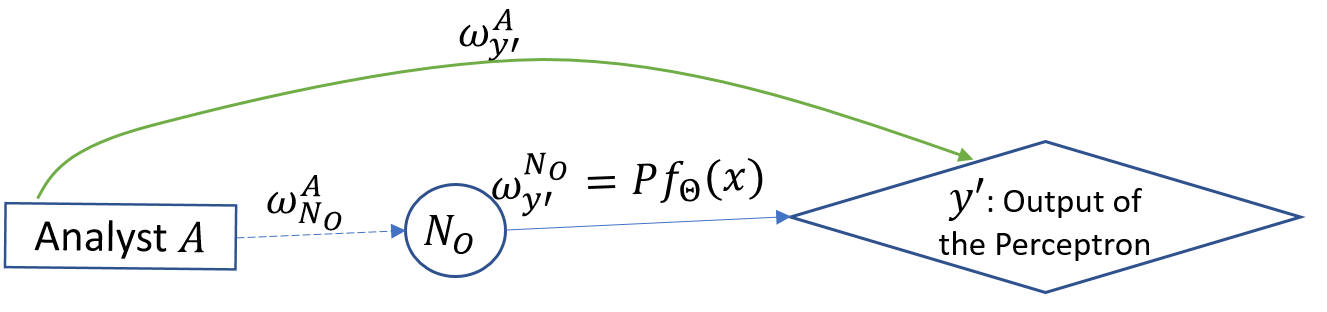
\includegraphics[scale=0.3]{img/pbstate.png}
    \caption{STN used to assess the output \(y\prime=f(x)\) of a perceptron \(\Theta\)}
    \label{fig:pbstate}
\end{figure}

% \subsection{Solution for the Perceptron}
\subsection{Trust Propagation from Input to Output}
% \todo[inline]{Describe Solution for Problem 1}
\begin{figure}
\centering
\subfloat[Perceptron for \cref{equ:smodel}]{
    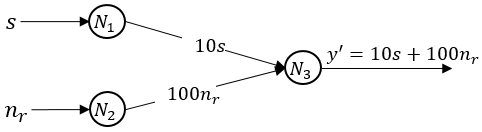
\includegraphics[width=0.35\textwidth]{img/NN1.png}
     \label{fig:nn1}
    }
   
\hfill
\subfloat[Parallel Trust Function for \cref{equ:smodel}]{
    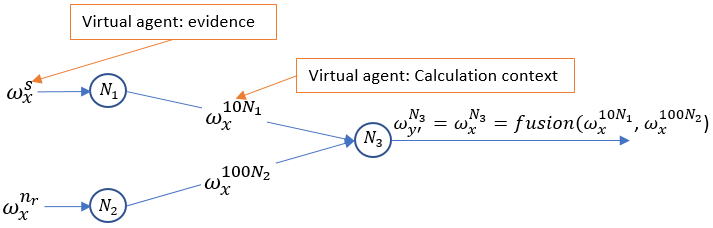
\includegraphics[width=0.45\textwidth]{img/NN1S.png}
   \label{fig:nn1s}}
\caption{Trust-propagation based solely on input-feature trust}
\label{fig:solution1}
\end{figure}
\noindent\paragraph*{Objective} Determine how trust in the individual input features (\(s\) and \(n_r\)) propagates through a simple perceptron to produce a trust assessment on the output variable \(y\prime\), representing the predicted apartment cost.
\paragraph*{Assumptions} For now, we assume that the model parameters \(\theta_1=10\) and  \(\theta_2=100\) are fully trusted and input feature trust opinions (\(T_s\) and \(T_{n_r}\)) are available.

The model specified in \cref{equ:smodel} is equivalent to the NN depicted in \cref{fig:nn1}. This network employs a linear transformation without an activation function. The input vector is:
$$ 
x = \begin{pmatrix}
    s \\
    n_r
\end{pmatrix}
$$ 
Let $\omega_x^s$ be the trust opinion on $x$ based on $s$ as evidence and  $\omega_x^{n_r}$ the trust opinion on $x$ based on $n_r$ as evidence. Since the output neuron $N_3$ computes \cref{equ:smodel}, we associate this computation with two agents: $10N_1$ from the context of computing \(10\cdot s\) and $100N_2$ from the context of computing \(100\cdot n_r\). The trust opinion of the output neuron \(N_3\) on \(x\) is then: 
\(\omega_x^{N_3} = \mathit{fusion}(\omega_x^{10N_1}, \omega_x^{100N_2})\). 

The choice of the fusion operator (that we will later denote by \(\oplus\) ) depends on the semantics of \(s\) and \(n_r\) (see Definition~\ref{def:fusion-app}). In this example, since $s$ and $n_r$ represent independent evidence, the fusion operator to use is cumulative fusion.

Assuming full trust in the parameters \(\theta_1 = 10\) and \(\theta_2 = 100\), we have:
\begin{align}
    \omega_x^{10N_1} = \omega_x^{N_1} = \omega_x^{s} = T_s \, \text{ (Trust in the feature \(s\) of \(x\))} \notag \\
    \omega_x^{100N_2} = \omega_x^{N_2} = \omega_x^{n_r} = T_{n_r} \, \text{ (Trust in the feature \(n_r\) of \(x\))} \notag 
\end{align}

Since the output value is deterministically related to the input via
\[
y' = f(x),
\]
the trust opinion of \(N_3\) on \(y'\) is the same as the trust opinion already computed for \(x\). Clearly, the transformation performed by \(f\) is encoded in the agent algebra, not in the variable algebra. Thus,
\begin{align}
    \omega_{y\prime}^{N_3} &= \omega_x^{N_3} = \omega_x^{10N_1} \oplus \omega_x^{100N_2} \notag \notag \\
&= \omega_x^{s} \oplus \omega_x^{n_r} = T_s \oplus T_{n_r}
\end{align}
In summary, if we define \(T_x = \begin{pmatrix}
    T_s&T_{n_r}
\end{pmatrix} \), then:
\[\pf_\Theta(T_x) = \pf_\Theta(\begin{pmatrix}
    T_s&T_{n_r}
\end{pmatrix}) =  T_s \oplus T_{n_r} \]


\subsection{Impact of Parameter Trust}
\paragraph*{Objective} Analyze how trust in the model parameters \(\theta_1=10\) and \(\theta_2=100\) affects the resulting trust assessment on the output \(y\prime\), given trust in the inputs.
\paragraph*{Assumption} Trust Opinions \(T_{\theta_1}\) and \(T_{\theta_2}\) are assigned to the parameters. The approach used to calculate these parameter-trust values will be discussed in Section~\ref{sec:patas}.

In problem 2, the model is expressed as:
\begin{equation}
    y\prime = \theta_1\times s + \theta_2\times n_r
    \label{equ:smodel2}
\end{equation} 
and we assume trust parameters \(T_{\theta_1}\) and \(T_{\theta_2}\) respectively in \(\theta_1\) and \(\theta_2\) (we'll see in details in Section~\ref{sec:patas} how to calculate these trust parameters). Unlike the previous problem, where we fully trusted \(\theta_1\) and \(\theta_2\), here we do not fully trust these parameters, and we must account for their trust assessments. For the network to incorporate the trust in \(\theta_1\) and \(\theta_2\), we adjust the trust opinions on the features accordingly. The trust opinions are now refined.
\begin{figure}
    \centering
    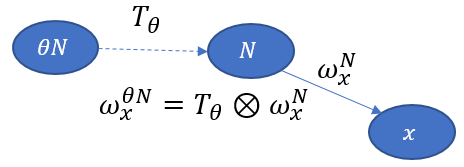
\includegraphics[width=0.4\linewidth]{img/multprob2.png}
    \caption{Trust-propagation Trust Network with parameter trust.}
    \label{fig:multprob2l}
\end{figure}
As depicted in \cref{fig:multprob2l}, we model this as a small subjective network. therefore:
\begin{align}
    \omega_x^{\theta_1 N_1} = T_{\theta_1} \otimes \omega_x^{N_1} \; \text{and} \;
    \omega_x^{\theta_1 N_2} =  T_{\theta_2} \otimes \omega_x^{N_2}
\end{align}
where \(\otimes\) is a trust discounting operator. This result is consistent with the solution for problem 1 as for fully trusted \(T_\theta=(1,0,0)\), we have \(\omega_x^{\theta N} = T_{\theta} \otimes \omega_x^{N} = \omega_x^{N}\) (for any neuron \(N\)).

Finally, the resulting output trust \(\omega_{y\prime}^{N_3}\) is calculated by the fusion of these adjusted trust opinions: 
\begin{equation}
\label{eq:sol222}
    \pf_\Theta(T_x) = \pf_\Theta(\begin{pmatrix}
    T_s&T_{n_r}
\end{pmatrix}) =  (T_{\theta_1}\otimes T_s)\oplus (T_{\theta_2}\otimes T_{n_r})
\end{equation}


Thus, we adjust the trust in the network output based on the trust in both the parameters and the features, ensuring that the trust propagation takes into account the trust in the parameters.



\section{Trust Node Structure}\label{app:trustnode}
\begin{figure}[H]
\centering
\begin{subfigure}{0.24\textwidth}
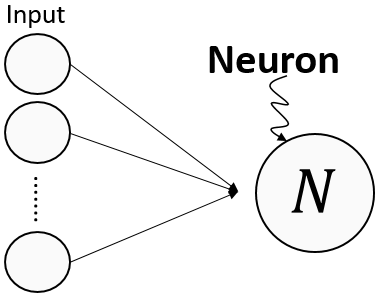
\includegraphics[width=\textwidth]{good_figs/trust_node/neuron.png}
  \caption{Structure of a Perceptron}
  \label{fig:neuron}
\end{subfigure}
\begin{subfigure}{0.24\textwidth}
  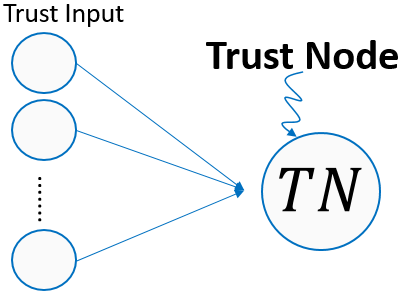
\includegraphics[width=\textwidth]{good_figs/trust_node/trustnode.png}
  \caption{Mirrored Trust Structure}
\end{subfigure}

\begin{subfigure}{0.48\textwidth}
  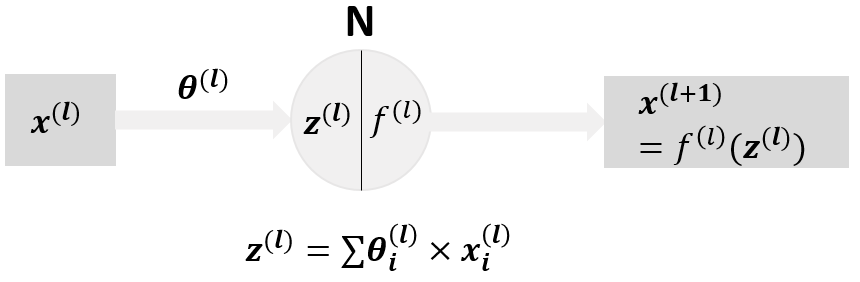
\includegraphics[width=\textwidth]{good_figs/trust_node/neurop.png}
  \caption{Perceptron Operation}
  \label{fig:neuronfunc}
\end{subfigure}
\begin{subfigure}{0.48\textwidth}
  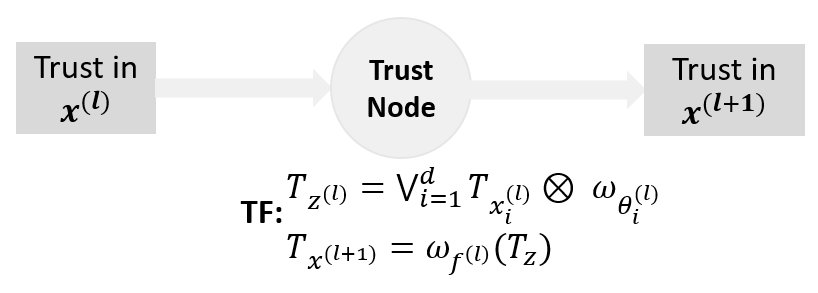
\includegraphics[width=\textwidth]{good_figs/trust_node/tnop.png}
  \caption{Trust Function Operation}
\end{subfigure}
\caption{Trust Node structure and computation, shown alongside the corresponding neuron operations.}
\label{fig:trustnodefull}
\end{figure}

\section{PaTAS Workflow and Functional Flow}\label{app:flow}
\begin{figure}[H]
    \centering
    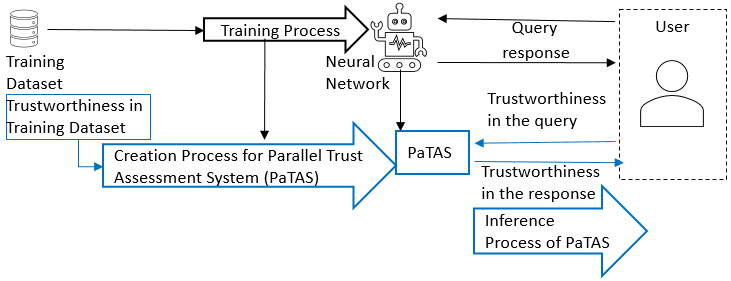
\includegraphics[width=0.75\linewidth]{screen/overviewPTAS.png}
    \caption{Overview of the PaTAS workflow.}
    \label{fig:ovvwptas}
\end{figure}

\begin{figure}[H]
    \centering
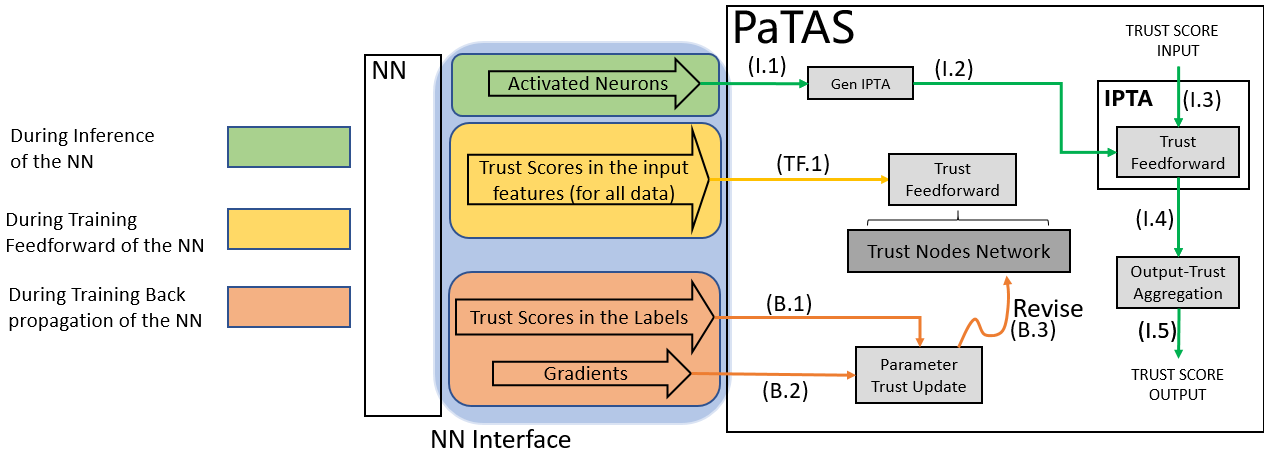
\includegraphics[width=0.85\linewidth]{good_figs/ptas/operations.png}

\caption{
    Functional flow of the PaTAS framework integrated with a neural network, illustrating how trust is propagated and revised during feedforward, backpropagation, and inference. 
    \\
    \textbf{Feedforward (Training Phase):} 
    The NN interface extracts trust scores from input features for all data being processed. These trust scores (TF.1) are passed to the \textit{Trust Feedforward} module, which propagates them through the \textit{Trust Nodes Network} in parallel with the neural computations. During training, Trust Feedforward also stores the trust scores of all intermediate computations in the NN, to be reused in backpropagation. 
    \\
    \textbf{Backpropagation (Training Phase):} 
    Once the NN computes gradients, the trust scores of the labels (B.1) and the gradients are provided to the \textit{Parameter-Trust Update}. Gradients (B.2) indicate how dataset labels affect parameter updates, while label trust determines whether these updates should be considered reliable. The stored intermediate trust values are also incorporated in this process. Finally, the \textit{Parameter-Trust Update} module refines the trust values of the Trust Nodes Network parameters (B.3), aligning them with the evolving learning dynamics. 
    \\
    \textbf{Inference Phase:} 
    During operation, contextual information such as the set of activated neurons is retrieved. This information is passed to \textit{GenIPTA} (I.1), which constructs an \textit{Inference Path Trust Assessment (IPTA)} corresponding to the specific inference path (I.2). The IPTA takes input trust scores (I.3), propagates them along the path, and produces trust scores for each NN output. These can then be passed to the \textit{Output-Trust Aggregation} (I.4) which will combine them into a single consolidated trust score representing the reliability of the prediction (I.5).
    }
    \label{fig:ptasoperation}
\end{figure}

\section{Helper Functions for \cref{alg:trustupdate}}\label{app:algorithm}
\begin{algorithm}[H]
\caption{Helper functions used by the Parameter-Trust Update}
\begin{algorithmic}[1]
    \Function{NodeTrust}{$g^{(l)}_i, T_{y_\text{batch}}, \epsilon$}
        \State Count $r$: \#edges with $|g^{(l)}_{i,j}| < \epsilon$ 
        \State Count $s$: \#edges with $|g^{(l)}_{i,j}| \geq \epsilon$ 
        \State Map $(r,s)$ into a binomial opinion using Baseline-Prior Quantification
        \State \Return $T_{n_i \mid y_\text{batch}}$
    \EndFunction

    \Function{DeduceTrust}{$T_{n_i \mid y_\text{batch}}, T_{n_i \mid \overline{y_\text{batch}}}, T_{y_\text{batch}}$}
        \State $T_{n_i \mid \overline{y_\text{batch}}}  \longleftarrow  (0,0,1)$
        \State \Return $T_{n_i \parallel Y_\text{batch}} = T_{y_\text{batch}} \circledcirc (T_{n_i \mid y_\text{batch}}, T_{n_i \mid \overline{y_\text{batch}}})$
    \EndFunction

    \Function{Revise}{$T_{\theta_{i,j}^{(l)}}, T_{n_i \parallel Y_\text{batch}}$}
        \State \Return $T_{\theta_{i,j}^{(l)}} \circleddash T_{n_i \parallel Y_\text{batch}}$
    \EndFunction
    \Function{Update}{$T_{\theta^{(l)}_{i,j}}, T_{lr}, 
    T_{x^{(l-1)}_j}, T_{y_\text{batch}}$}
    \State \Return $T_{\theta^{(l)}_{i,j}} \odot 
           (T_{x^{(l-1)}_j} \oslash T_{y_\text{batch}})$
    \EndFunction

\end{algorithmic}
\end{algorithm}

\section{Perturbation Functions Used in \cref{exp:1}}\label{app:perturb}
In practice, feature and label trust degradation may arise from poor-quality imaging, human annotation errors, or flaws in the preprocessing pipeline. 
In all experiments, we simulate degradations using controlled perturbation functions. 
For fully uncertain feature opinion, we introduce additive uniform noise 
\vspace{-1em}
\[
x' = x + \mu, \quad \mu \sim U(-\eta, \eta),
\]
where 
\(
\eta = 0.3 \times \max(\text{features}).
\)
Each feature is perturbed with probability $0.3$. 
After noise addition, if $x'$ lies outside the valid range 
$[\min(\text{features}), \max(\text{features})]$, it is clipped to the corresponding boundary:
\[
x' = 
\begin{cases}
\min(\text{features}), & x' < \min(\text{features}), \\
\max(\text{features}), & x' > \max(\text{features}), \\
x', & \text{otherwise}.
\end{cases}
\]
To model distrust, we generate corrupted inputs by sampling from a uniform distribution over the feature space:
\[
x' \sim U(\min(\text{features}), \max(\text{features})),
\]

Label degradation is modeled analogously: uncertainty is introduced via random label noise, while full distrust is represented by a complete replacement of the labels.

\section{Conformity-Based Input-Trust Construction (\cref{exp:4})}\label{app:conformity}
This appendix specifies the input-trust construction used in \cref{exp:4} precisely; all parameters are fixed once and shared by every dataset.

Let the clean training features be $x^{(1)},\dots,x^{(n)} \in \mathbb{R}^m$. For each feature $j$ we compute the marginal mean $\mu_j$ and standard deviation $\sigma_j$, and a robust span $S$ of the whole feature matrix as the difference between its $99.5$th and $0.5$th percentiles. The \emph{effective deviation} is floored at a fraction of the span,
\[
\sigma^{\mathrm{eff}}_j = \max(\sigma_j,\, 0.02\, S),
\]
so that near-constant features cannot produce unbounded standardized deviations from minimal perturbations. For an input $x$, the standardized deviation is $z_j = |x_j - \mu_j| / \sigma^{\mathrm{eff}}_j$ and the conformity is
\[
g_j = \exp\!\big(-\tfrac{1}{2}\max(z_j - 1,\, 0)^2\big) \in (0,1],
\]
so deviations within one effective standard deviation are fully conforming and only the excess erodes conformity. The \emph{reliability weight} of feature $j$ is the capped inverse-variance weight
\[
w_j = \min\!\big((\sigma_{\mathrm{ref}} / \sigma^{\mathrm{eff}}_j)^2,\, 64\big),
\qquad \sigma_{\mathrm{ref}} = \operatorname{median}_j \sigma^{\mathrm{eff}}_j,
\]
expressing that a feature with a tight training distribution is a reliable witness whose violation is unambiguous, while the cap bounds the influence any single feature can exert. Each feature contributes evidence $r_j = N w_j g_j$ and $s_j = N w_j (1-g_j)$ with base evidence mass $N = 50$, mapped to a binomial opinion by \cref{eq:q1} with $W = 2$; this is the same quantification used for parameter trust. The per-sample input trust $P_{\mathrm{input}}$ is the projected probability (base rate $0.5$) of the pooled opinion obtained by applying \cref{eq:q1} to the summed evidence $(\sum_j r_j, \sum_j s_j)$, which corresponds to cumulative fusion of independent evidence sources.

The columns of \cref{tab:diagnostics} are, in this notation: the median of $\sigma^{\mathrm{eff}}_j$, the maximum of $w_j$, the share of total weight mass held by the top decile of features ranked by $w_j$, and the fraction of features with $w_j \geq 4$. The last two are descriptive statistics of weight concentration used for reporting only (the threshold $w_j \geq 4$ corresponds to $\sigma^{\mathrm{eff}}_j$ at most half of $\sigma_{\mathrm{ref}}$); they are not parameters of the construction.

\vspace{-0.5em}
\section{Operator and Threshold Sensitivity}\label{app:ablations}
Both ablations use the MNIST 784-128-10 trust/trust scenario of \cref{exp:2} (20 epochs, 1000-sample evaluation subset, test-time feature noise $p = 0.3$ for the noisy columns).

\Cref{tab:abl-fusion} varies the trust-revision fusion operator. The converged trust mass and every downstream metric agree to within $0.002$ across averaging, cumulative, and weighted fusion, so the findings of this paper do not depend on the variant; averaging is used throughout because Theorem~\ref{thm:arithm} establishes non-degenerate long-run behavior under repeated revision, whereas cumulative fusion accumulates evidence monotonically toward dogmatic (zero-uncertainty) opinions.

\Cref{tab:abl-eps} sweeps the gradient-evidence threshold over three orders of magnitude. The trusted-input trust mass and the selective-prediction metrics are constant on the plateau $\epsilon \in [0.05, 1]$ and degrade only at degenerate-small values, where nearly every gradient is read as strong evidence; the equality of the trusted-input trust and distrusted-input distrust columns is the belief/disbelief symmetry of Theorem~\ref{thm:infvac} observed empirically.

\begin{table}[H]
\centering\footnotesize
\begin{tabular}{lccccc}
\toprule
Fusion & Trust $t_{\mathrm{tr}}$ & AUROC$_{\mathrm{cl}}$ & AUROC$_{\mathrm{no}}$ & ECE$_{\mathrm{cl}}$ & ECE$_{\mathrm{no}}$ \\
\midrule
Average (used) & 0.988 & 0.957 & 0.973 & 0.013 & 0.020 \\
Cumulative & 0.990 & 0.957 & 0.973 & 0.012 & 0.020 \\
Weighted & 0.989 & 0.957 & 0.973 & 0.013 & 0.020 \\
\bottomrule
\end{tabular}
\caption{Trust-revision fusion ablation: converged trusted-input trust mass and selective-prediction metrics on clean (cl) and feature-noised (no) test data.}
\label{tab:abl-fusion}
\end{table}

\begin{table}[H]
\centering\footnotesize
\begin{tabular}{lccccc}
\toprule
$\epsilon$ & $t_{\mathrm{tr}}$ & $d_{\mathrm{dis}}$ & AUROC$_{\mathrm{cl}}$ & AUROC$_{\mathrm{no}}$ & ECE$_{\mathrm{cl}}$ \\
\midrule
0.001 & 0.573 & 0.573 & 0.826 & 0.900 & 0.195 \\
0.01 & 0.976 & 0.976 & 0.940 & 0.964 & 0.018 \\
0.05$^{*}$ & 0.989 & 0.989 & 0.957 & 0.973 & 0.013 \\
0.1 & 0.989 & 0.989 & 0.957 & 0.973 & 0.013 \\
0.2 & 0.989 & 0.989 & 0.957 & 0.973 & 0.013 \\
0.5 & 0.989 & 0.989 & 0.957 & 0.973 & 0.013 \\
1.0 & 0.989 & 0.989 & 0.957 & 0.973 & 0.013 \\
\bottomrule
\end{tabular}
\caption{$\epsilon$ sweep ($^{*}$ = value used in Experiments 2--4): trusted-input trust $t_{\mathrm{tr}}$, distrusted-input distrust $d_{\mathrm{dis}}$ (equal by Theorem~\ref{thm:infvac}), and selective-prediction metrics. All quantities are constant on $\epsilon \in [0.05, 1]$.}
\label{tab:abl-eps}
\end{table}

\section{Detailed results}\label{app:expres}

\begin{figure}[H]
\centering
\begin{subfigure}{0.72\linewidth}
    \centering
    \includegraphics[width=\linewidth]{main_plots/plot_ptas-128-t-t-ps4.pdf}
    \caption{Trust mass}
    \label{fig:4x4}
\end{subfigure}
\begin{subfigure}{0.72\linewidth}
    \centering
    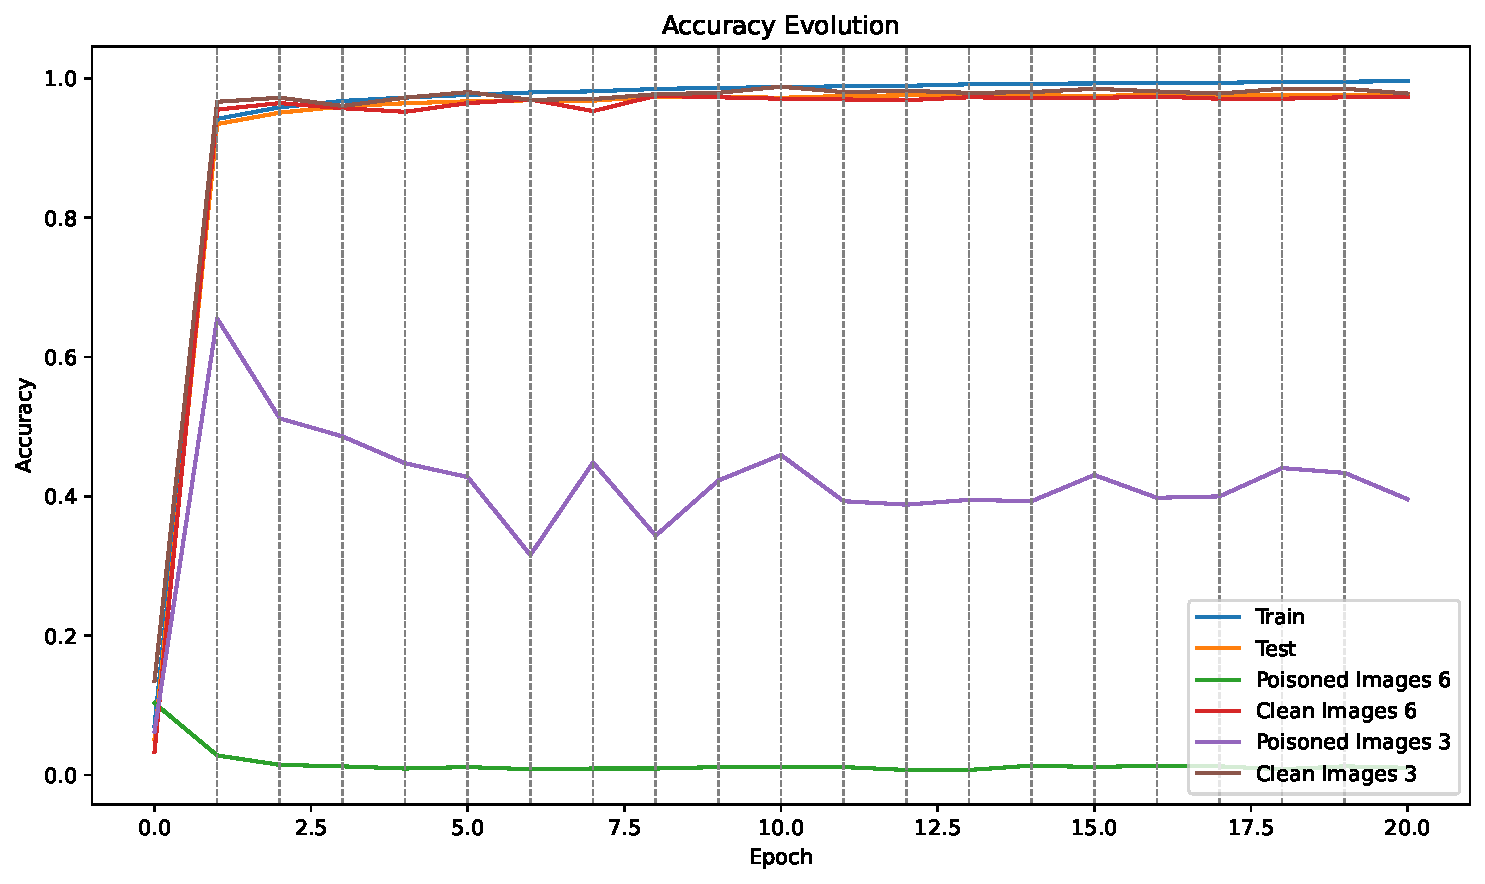
\includegraphics[width=\linewidth]{main_plots/accuracy_evolution-128-t-t-ps4.pdf}
    \caption{Accuracy}
    \label{fig:4x4acc}
\end{subfigure}
\caption{Evolution of trust mass and accuracy for a fully trusted input, MNIST poisoned experiment, patch size \(4\times4\).}
\label{fig:4x4both}
\end{figure}

All the results are depicted in Figures in \cref{sec:rescancer0.01,sec:rescancer0.1,sec:resmnistaccapp,sec:resmnist,sec:resmnistpois,sec:resrand}.
\begin{itemize}
\item \emph{Fully Trusted Input}: where the trust in the data is considered trusted (row 1 in each figure).
\item \emph{Fully Uncertain Input}: where the trust in the data is considered uncertain (row 2 in each figure).
\item \emph{Fully Distrusted Input}: where the data is assumed to be unreliable (row 3 in each figure).
\end{itemize}

% \subsection{Plots for Cancer Model with \(\epsilon = 0.01\) (\cref{exp:1})}\label{sec:rescancer0.01}

\begin{figure}[H]
  \includegraphics[width=\textwidth]{plots_v2/Cancer/eps=0.1/plot_ptas-d-d.pdf}
  \caption{xdistrust+ydistrust}
\end{figure}

\begin{figure}[H]
  
\includegraphics[width=\textwidth]{good_plots/cancer/hidden=16/eps=0.01/xdistrustyvacuous/all.pdf}
  \caption{xdistrust+yvacuous}
\end{figure}
\begin{figure}[H]
  
\includegraphics[width=\textwidth]{good_plots/cancer/hidden=16/eps=0.01/xdistrustytrust/all.pdf}
  \caption{xdistrust+ytrust}
\end{figure}
\begin{figure}[H]
  
\includegraphics[width=\textwidth]{good_plots/cancer/hidden=16/eps=0.01/xvacuousydistrust/all.pdf}
  \caption{xvacuous+ydistrust}
\end{figure}
\begin{figure}[H]
  
\includegraphics[width=\textwidth]{good_plots/cancer/hidden=16/eps=0.01/xvacuousyvacuous/all.pdf}
  \caption{xvacuous+yvacuous}
\end{figure}
\begin{figure}[H]
  
\includegraphics[width=\textwidth]{good_plots/cancer/hidden=16/eps=0.01/xvacuousytrust/all.pdf}
  \caption{xvacuous+ytrust}
\end{figure}
\begin{figure}[H]
  
\includegraphics[width=\textwidth]{good_plots/cancer/hidden=16/eps=0.01/xtrustydistrust/all.pdf}
  \caption{xtrust+ydistrust}
\end{figure}
\begin{figure}[H]
  
\includegraphics[width=\textwidth]{good_plots/cancer/hidden=16/eps=0.01/xtrustyvacuous/all.pdf}
  \caption{xtrust+yvacuous}
\end{figure}
\begin{figure}[H]
  
\includegraphics[width=\textwidth]{good_plots/cancer/hidden=16/eps=0.01/xtrustytrust/all.pdf}
  \caption{xtrust+ytrust}
\end{figure}



\subsection{Cancer Model with \( \epsilon = 0.1 \)(\cref{exp:1})}\label{sec:rescancer0.1}


\begin{figure}[H]
  
\includegraphics[width=\textwidth]{good_plots/cancer/hidden=16/eps=0.1/xdistrustydistrust/all.pdf}
  \caption{xdistrust+ydistrust}
\end{figure}
\begin{figure}[H]
  
\includegraphics[width=\textwidth]{good_plots/cancer/hidden=16/eps=0.1/xdistrustyvacuous/all.pdf}
  \caption{xdistrust+yvacuous}
\end{figure}
\begin{figure}[H]
  
\includegraphics[width=\textwidth]{good_plots/cancer/hidden=16/eps=0.1/xdistrustytrust/all.pdf}
  \caption{xdistrust+ytrust}
\end{figure}
\begin{figure}[H]
  
\includegraphics[width=\textwidth]{good_plots/cancer/hidden=16/eps=0.1/xvacuousydistrust/all.pdf}
  \caption{xvacuous+ydistrust}
\end{figure}
\begin{figure}[H]
  
\includegraphics[width=\textwidth]{good_plots/cancer/hidden=16/eps=0.1/xvacuousyvacuous/all.pdf}
  \caption{xvacuous+yvacuous}
\end{figure}
\begin{figure}[H]
  
\includegraphics[width=\textwidth]{good_plots/cancer/hidden=16/eps=0.1/xvacuousytrust/all.pdf}
  \caption{xvacuous+ytrust}
\end{figure}
\begin{figure}[H]
  
\includegraphics[width=\textwidth]{good_plots/cancer/hidden=16/eps=0.1/xtrustydistrust/all.pdf}
  \caption{xtrust+ydistrust}
\end{figure}
\begin{figure}[H]
  
\includegraphics[width=\textwidth]{good_plots/cancer/hidden=16/eps=0.1/xtrustyvacuous/all.pdf}
  \caption{xtrust+yvacuous}
\end{figure}
\begin{figure}[H]
  
\includegraphics[width=\textwidth]{good_plots/cancer/hidden=16/eps=0.1/xtrustytrust/all.pdf}
  \caption{xtrust+ytrust}
\end{figure}




\subsection{Results for trust Degradation (\cref{exp:1})}\label{sec:resdegradation}

\begin{figure}[H]
  
\includegraphics[width=\textwidth]{good_plots/cancer/hidden=16/025-0-075/all.pdf}
  \caption{(0.25, 0, 0.75)}
\end{figure}
\begin{figure}[H]
  
\includegraphics[width=\textwidth]{good_plots/cancer/hidden=16/025-025-050/all.pdf}
  \caption{(0.25, 0.25, 0.5)}
\end{figure}
    





% 


\subsection{Accuracy Evolution for the Cancer Model (\cref{exp:1})}\label{sec:resmnistaccapp}
\begin{figure}[H]
\centering
\begin{subfigure}[b]{0.32\textwidth}
  
\includegraphics[width=\textwidth]{good_plots/accuracy/Cancer/0.3-0.5/Cancer-clean-clean.pdf}
  \caption{Clean Features and Labels}
\end{subfigure}
\begin{subfigure}[b]{0.32\textwidth}
  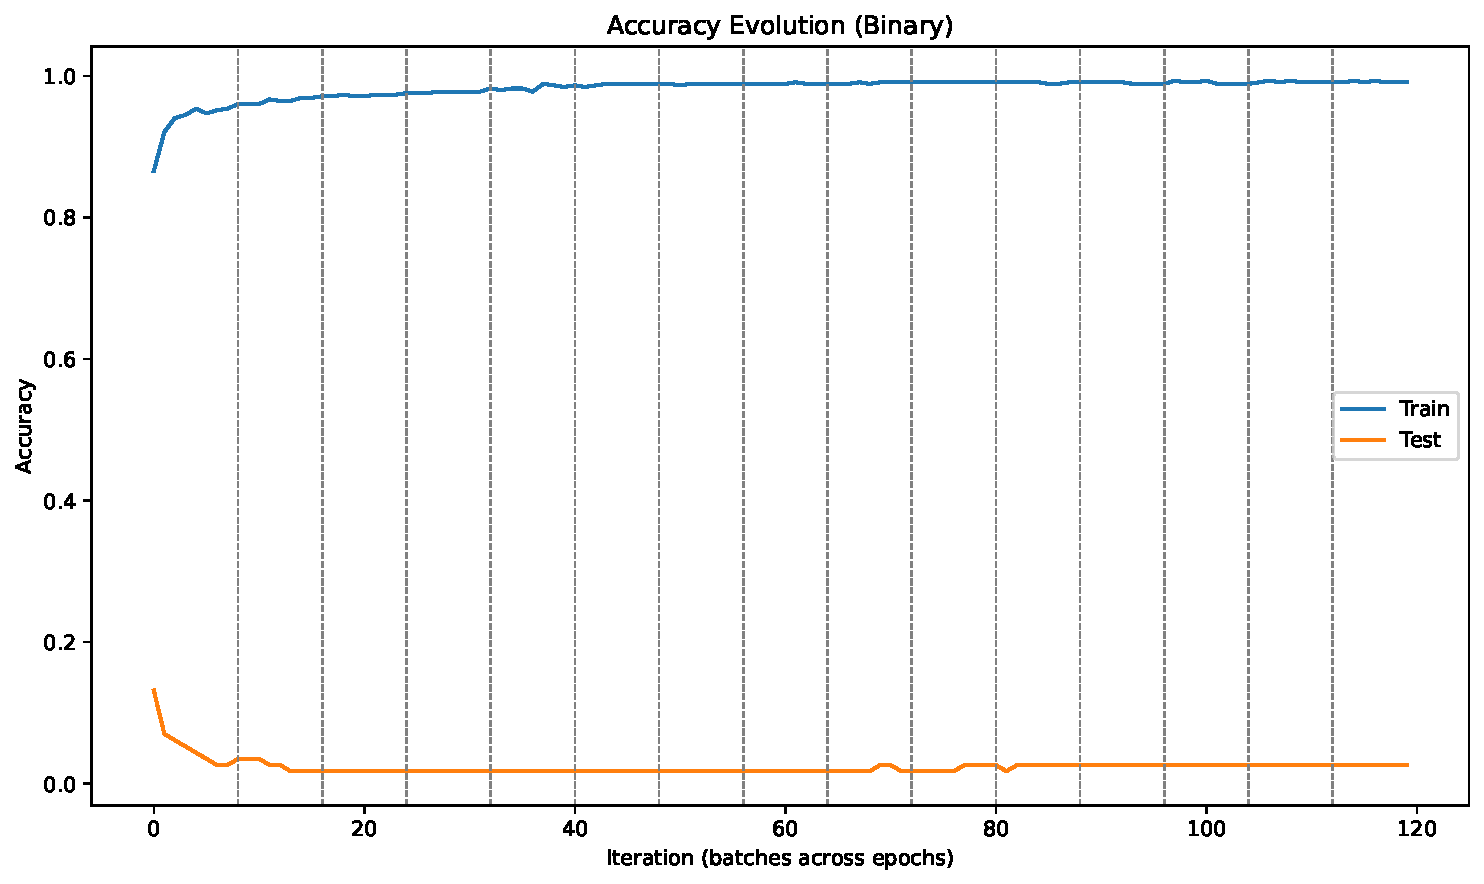
\includegraphics[width=\textwidth]{plots_v2/Cancer/eps=0.01/accuracy_evolution-t-d.pdf}
  \caption{Clean Features and Corrupted Labels}
\end{subfigure}
\begin{subfigure}[b]{0.32\textwidth}
  
\includegraphics[width=\textwidth]{good_plots/accuracy/Cancer/0.3-0.5/Cancer-clean-noise.pdf}
  \caption{Clean Features and Noisy Labels}
\end{subfigure}
\begin{subfigure}[b]{0.32\textwidth}
  
\includegraphics[width=\textwidth]{good_plots/accuracy/Cancer/0.3-0.5/Cancer-noise-clean.pdf}
  \caption{Noisy Features and Clean Labels}
\end{subfigure}
\begin{subfigure}[b]{0.32\textwidth}
  
\includegraphics[width=\textwidth]{good_plots/accuracy/Cancer/0.3-0.5/Cancer-noise-corrupt.pdf}
  \caption{Noisy Features and Corrupted Labels}
\end{subfigure}
\begin{subfigure}[b]{0.32\textwidth}
  
\includegraphics[width=\textwidth]{good_plots/accuracy/Cancer/0.3-0.5/Cancer-noise-noise.pdf}
  \caption{Noisy Features and Noisy Labels}
\end{subfigure}
\begin{subfigure}[b]{0.32\textwidth}
  
\includegraphics[width=\textwidth]{good_plots/accuracy/Cancer/0.3-0.5/Cancer-corrupt-clean.pdf}
  \caption{Corrupted Features and Clean Labels}
\end{subfigure}
\begin{subfigure}[b]{0.32\textwidth}
  
\includegraphics[width=\textwidth]{good_plots/accuracy/Cancer/0.3-0.5/Cancer-corrupt-corrupt.pdf}
  \caption{Corrupted Features and Corrupted Labels}
\end{subfigure}
\begin{subfigure}[b]{0.32\textwidth}
  
\includegraphics[width=\textwidth]{good_plots/accuracy/Cancer/0.3-0.5/Cancer-corrupt-noise.pdf}
  \caption{Corrupted Features and Noisy Labels}
\end{subfigure}
\caption{Accuracy evolution of the Cancer model under different combinations of clean, corrupted, and noisy features and labels.}
\label{fig:Acccancer}
\end{figure}

\begin{figure}[H]
    \centering
    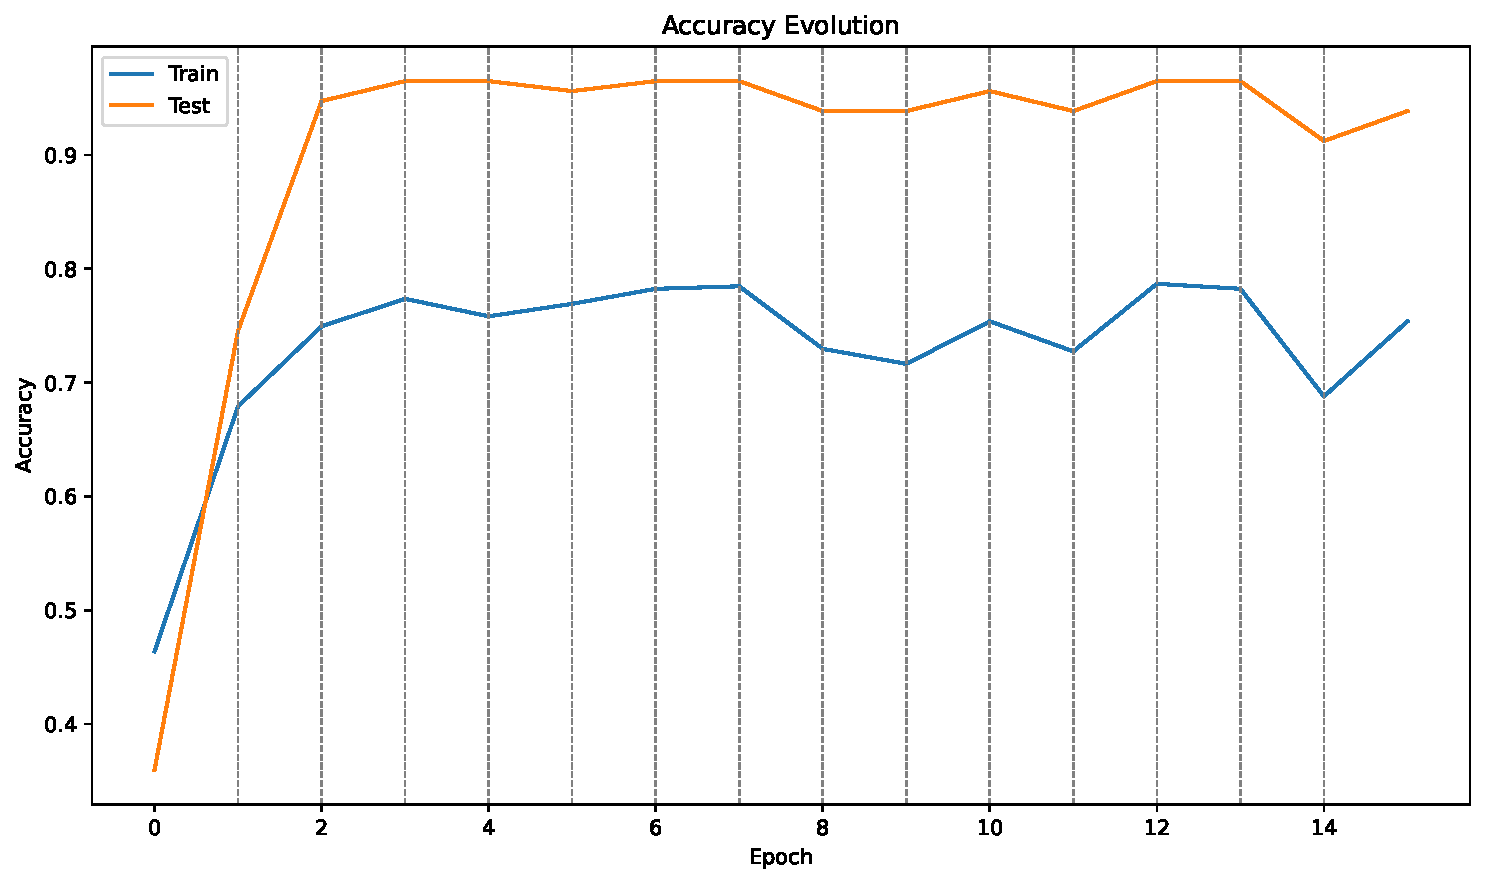
\includegraphics[width=0.8\linewidth]{good_plots/accuracy/Cancer/0.15-0.25/Cancer-noise-noise.pdf}
    \caption{Accuracy evolution of the Cancer model when reducing the noise for noised features and labels.}
    \label{fig:AcccancerInt}
\end{figure}





% \subsection{MNIST with Vacuous Trust Assessment (\cref{exp:2})}\label{sec:resmnist}
% \begin{figure}[H]
%   \centering
%   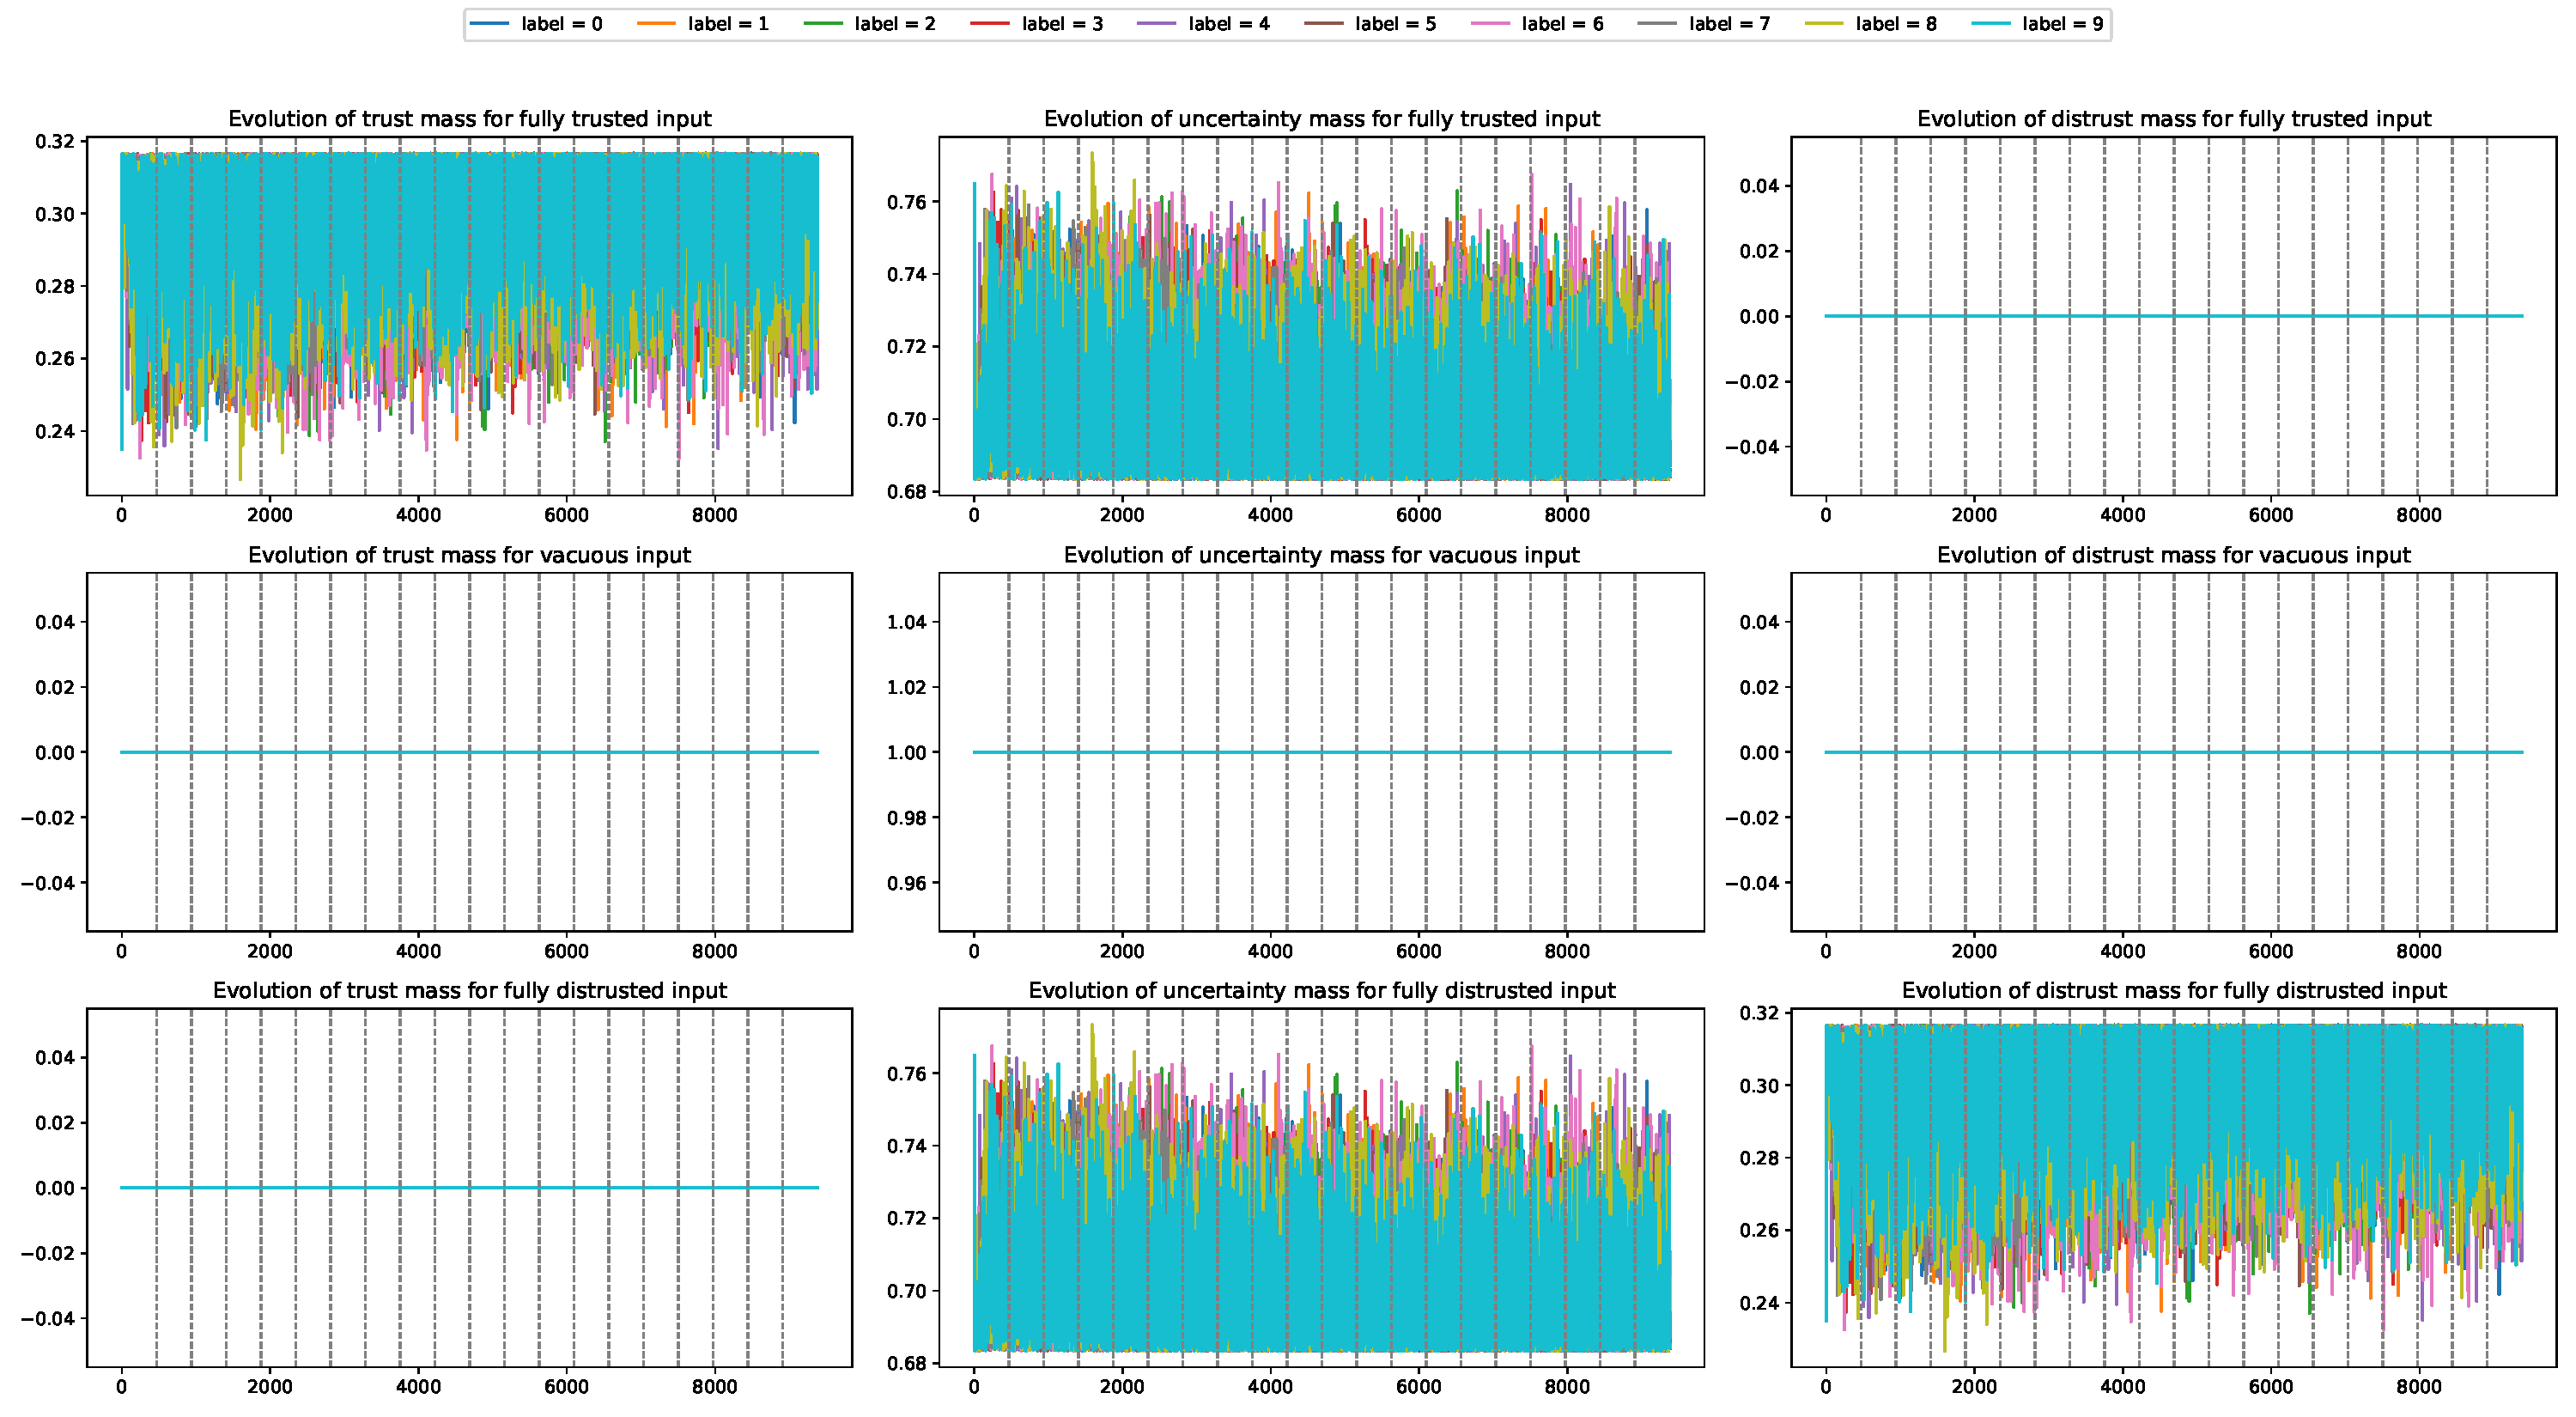
\includegraphics[width=\textwidth]{plots_v2/MNIST/architecture/plot_ptas-16-v-v.pdf}
%   \caption{16 Hidden neurons}
% \end{figure}
% \begin{figure}[H]
%   \centering
%   
\includegraphics[width=\textwidth]{good_plots/MNIST/hidden=20/xvacuousyvacuous/all.pdf}
%   \caption{20 Hidden neurons}
% \end{figure}
% \begin{figure}[H]
%   \centering
%   
\includegraphics[width=\textwidth]{good_plots/MNIST/hidden=20/xtrustytrust/all.pdf}
%   \caption{20 Hidden neurons with Fully Trusted Assessment}
% \end{figure}



% \begin{figure}[H]
% \centering
% \begin{subfigure}[b]{0.49\textwidth}
%   \centering
%   
\includegraphics[width=\textwidth]{good_plots/accuracy/MNIST/hiddenSize/5.pdf}
%   \caption{5 Hidden neurons}
% \end{subfigure}
% \begin{subfigure}[b]{0.49\textwidth}
%   \centering
%   
\includegraphics[width=\textwidth]{good_plots/accuracy/MNIST/hiddenSize/10.pdf}
%   \caption{10 Hidden neurons}
% \end{subfigure}
% \begin{subfigure}[b]{0.49\textwidth}
%   \centering
%   
\includegraphics[width=\textwidth]{good_plots/accuracy/MNIST/hiddenSize/20.pdf}
%   \caption{20 Hidden neurons}
% \end{subfigure}
% \begin{subfigure}[b]{0.49\textwidth}
%   \centering
%   
\includegraphics[width=\textwidth]{good_plots/accuracy/MNIST/hiddenSize/20T.pdf}
%   \caption{20 Hidden neurons with Fully Trusted Assessment}
% \end{subfigure}
% \caption{MNIST with Vacuous Trust Assessment}
% \label{fig:mnist}
% \end{figure}

% \subsection{MNIST poisoned 128 hidden neurons (\cref{exp:3})}\label{sec:resmnistpois}
% \begin{figure}[H]
%   \centering
%   
\includegraphics[width=\textwidth]{good_plots/MNIST/pois_hidden=20/1/all.pdf}
%   \caption{1 pixel}
% \end{figure}
% \begin{figure}[H]
%   \centering
%   
\includegraphics[width=\textwidth]{good_plots/MNIST/pois_hidden=20/4/all.pdf}
%   \caption{4×4 pixels}
% \end{figure}

% \begin{figure}[H]
%   \centering
%   
\includegraphics[width=\textwidth]{good_plots/MNIST/pois_hidden=20/20/all.pdf}
%   \caption{20×20 pixels}
% \end{figure}
% \begin{figure}[H]
%   \centering
%   
\includegraphics[width=\textwidth]{good_plots/MNIST/pois_hidden=20/27/all.pdf}
%   \caption{27×27 pixels}
% \end{figure}



% \begin{figure}[H]
% \centering
% \begin{subfigure}{0.5\textwidth}
%   \centering
%   
\includegraphics[width=\textwidth]{good_plots/accuracy/MNIST/poisoned/MNIST1.pdf}
%   \caption{1 pixel}
% \end{subfigure}
% \begin{subfigure}{0.5\textwidth}
%   \centering
%   
\includegraphics[width=\textwidth]{good_plots/accuracy/MNIST/poisoned/MNIST4.pdf}
%   \caption{4×4 pixels}
% \end{subfigure}
% \\
% \begin{subfigure}{0.5\textwidth}
%   \centering
%   
\includegraphics[width=\textwidth]{good_plots/accuracy/MNIST/poisoned/MNIST20.pdf}
%   \caption{20×20 pixels}
% \end{subfigure}
% \begin{subfigure}{0.5\textwidth}
%   \centering
%   
\includegraphics[width=\textwidth]{good_plots/accuracy/MNIST/poisoned/MNIST27.pdf}
%   \caption{27×27 pixels}
% \end{subfigure}
% \caption{Accuracy for poisoned MNIST model with 20 hidden neurons}
% \label{fig:mnistpoisacc}
% \end{figure}



\subsection{Plots for Cancer Model with \(\epsilon = 0.01\) (\cref{exp:1})}\label{sec:rescancer0.01}
\begin{figure}[H]
  \includegraphics[width=\textwidth]{plots_v2/Cancer/eps=0.01/plot_ptas-d-d.pdf}
  \caption{Features distrusted and labels distrusted}
\end{figure}
\begin{figure}[H]
  \includegraphics[width=\textwidth]{plots_v2/Cancer/eps=0.01/plot_ptas-d-v.pdf}
  \caption{Features distrusted and labels vacuous}
\end{figure}
\begin{figure}[H]
  \includegraphics[width=\textwidth]{plots_v2/Cancer/eps=0.01/plot_ptas-d-t.pdf}
  \caption{Features distrusted and labels trusted}
\end{figure}
\begin{figure}[H]
  \includegraphics[width=\textwidth]{plots_v2/Cancer/eps=0.01/plot_ptas-v-d.pdf}
  \caption{Features vacuous and labels distrusted}
\end{figure}
\begin{figure}[H]
  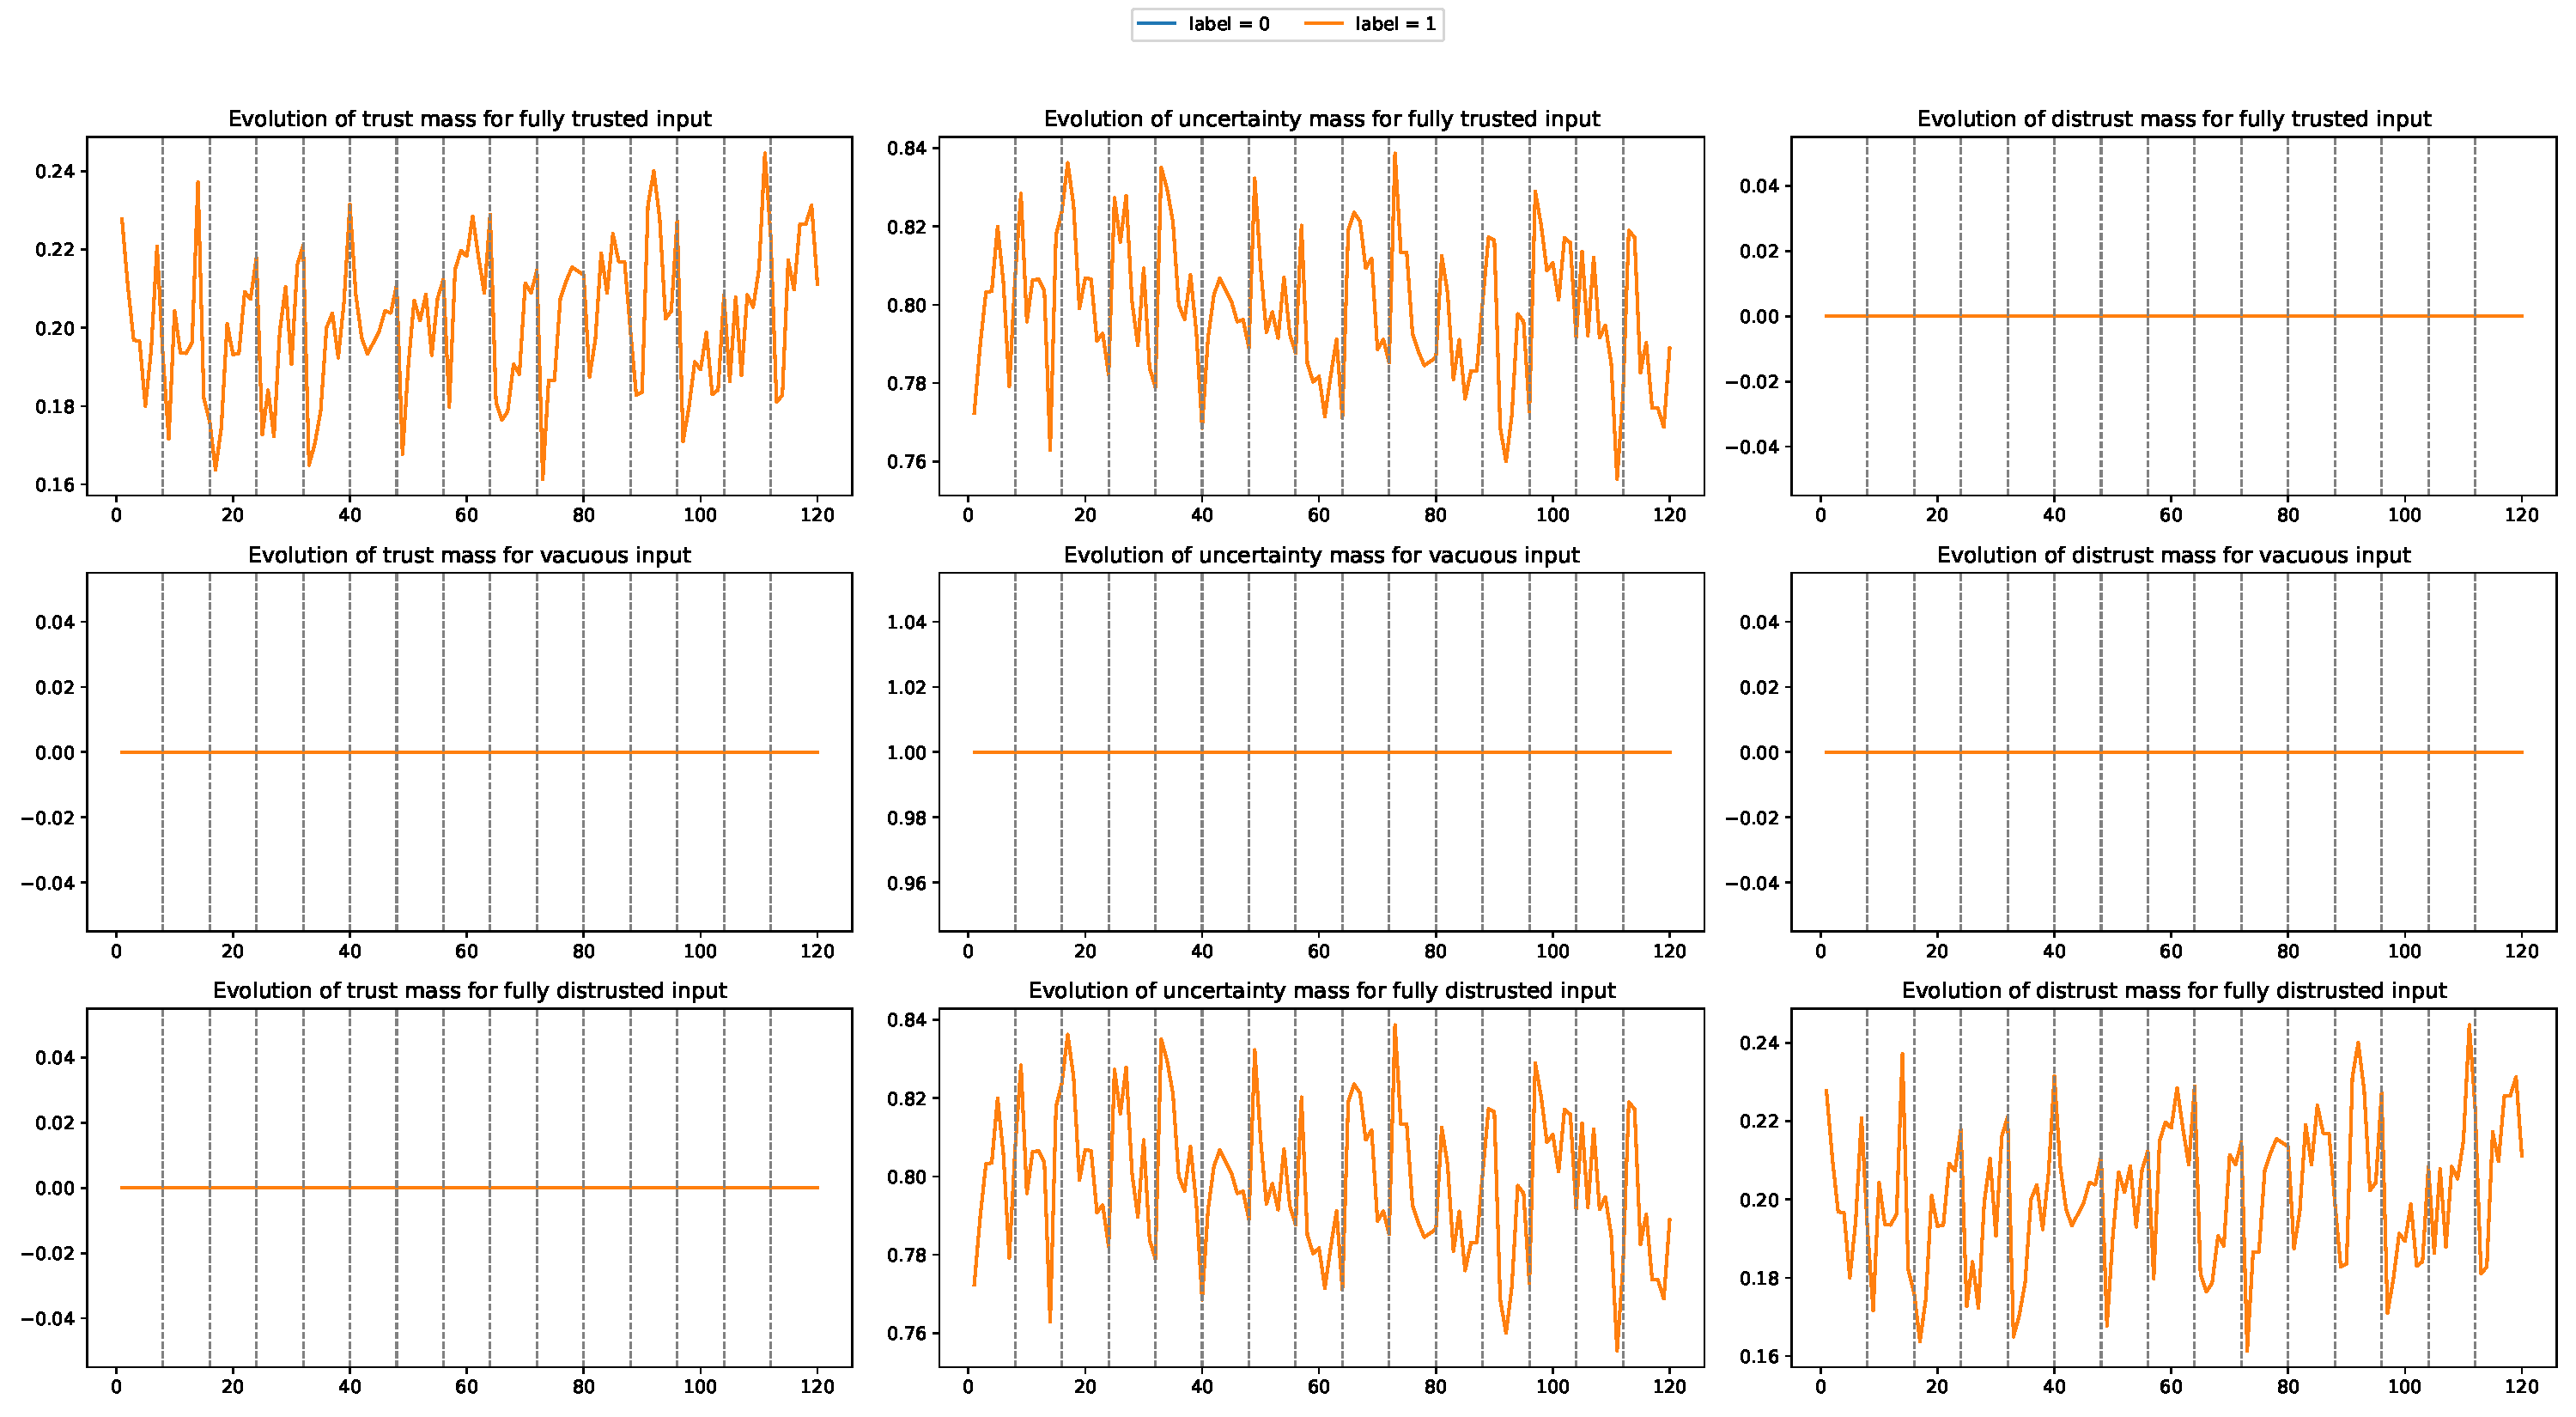
\includegraphics[width=\textwidth]{plots_v2/Cancer/eps=0.01/plot_ptas-v-v.pdf}
  \caption{Features vacuous and labels vacuous}
\end{figure}
\begin{figure}[H]
  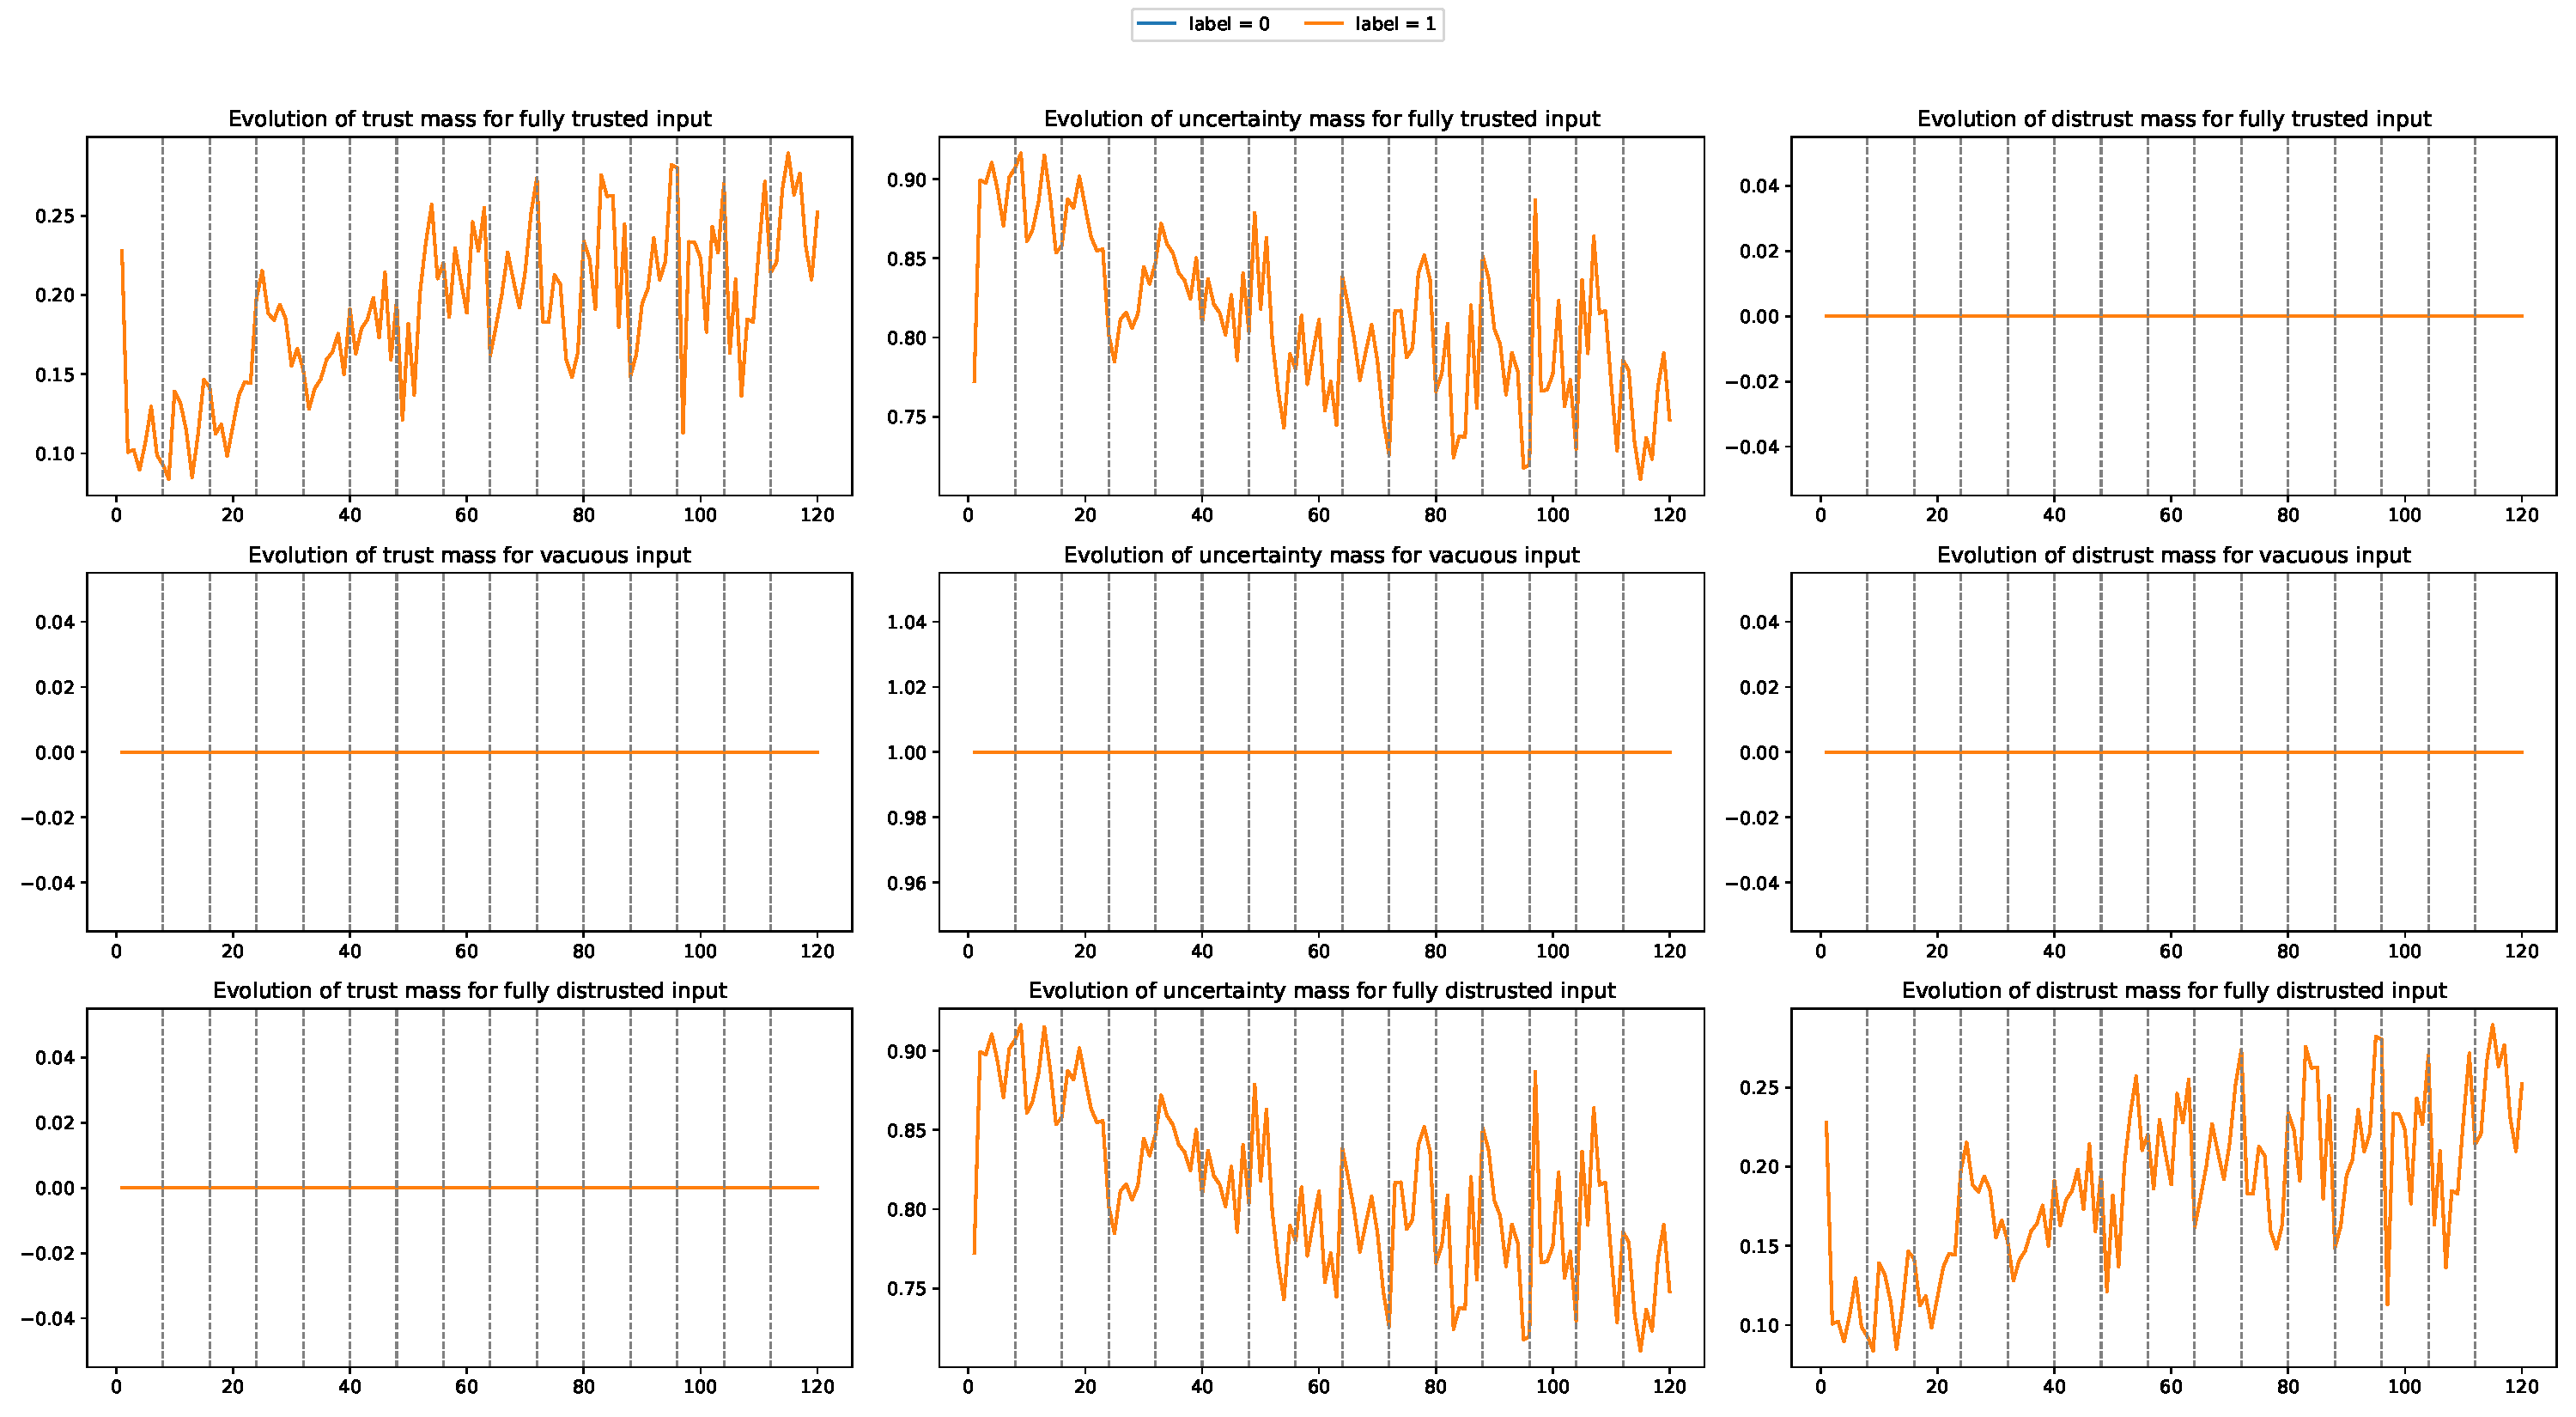
\includegraphics[width=\textwidth]{plots_v2/Cancer/eps=0.01/plot_ptas-v-t.pdf}
  \caption{Features vacuous and labels trusted}
\end{figure}
\begin{figure}[H]
  \includegraphics[width=\textwidth]{plots_v2/Cancer/eps=0.01/plot_ptas-t-d.pdf}
  \caption{Features trusted and labels distrusted}
\end{figure}
\begin{figure}[H]
  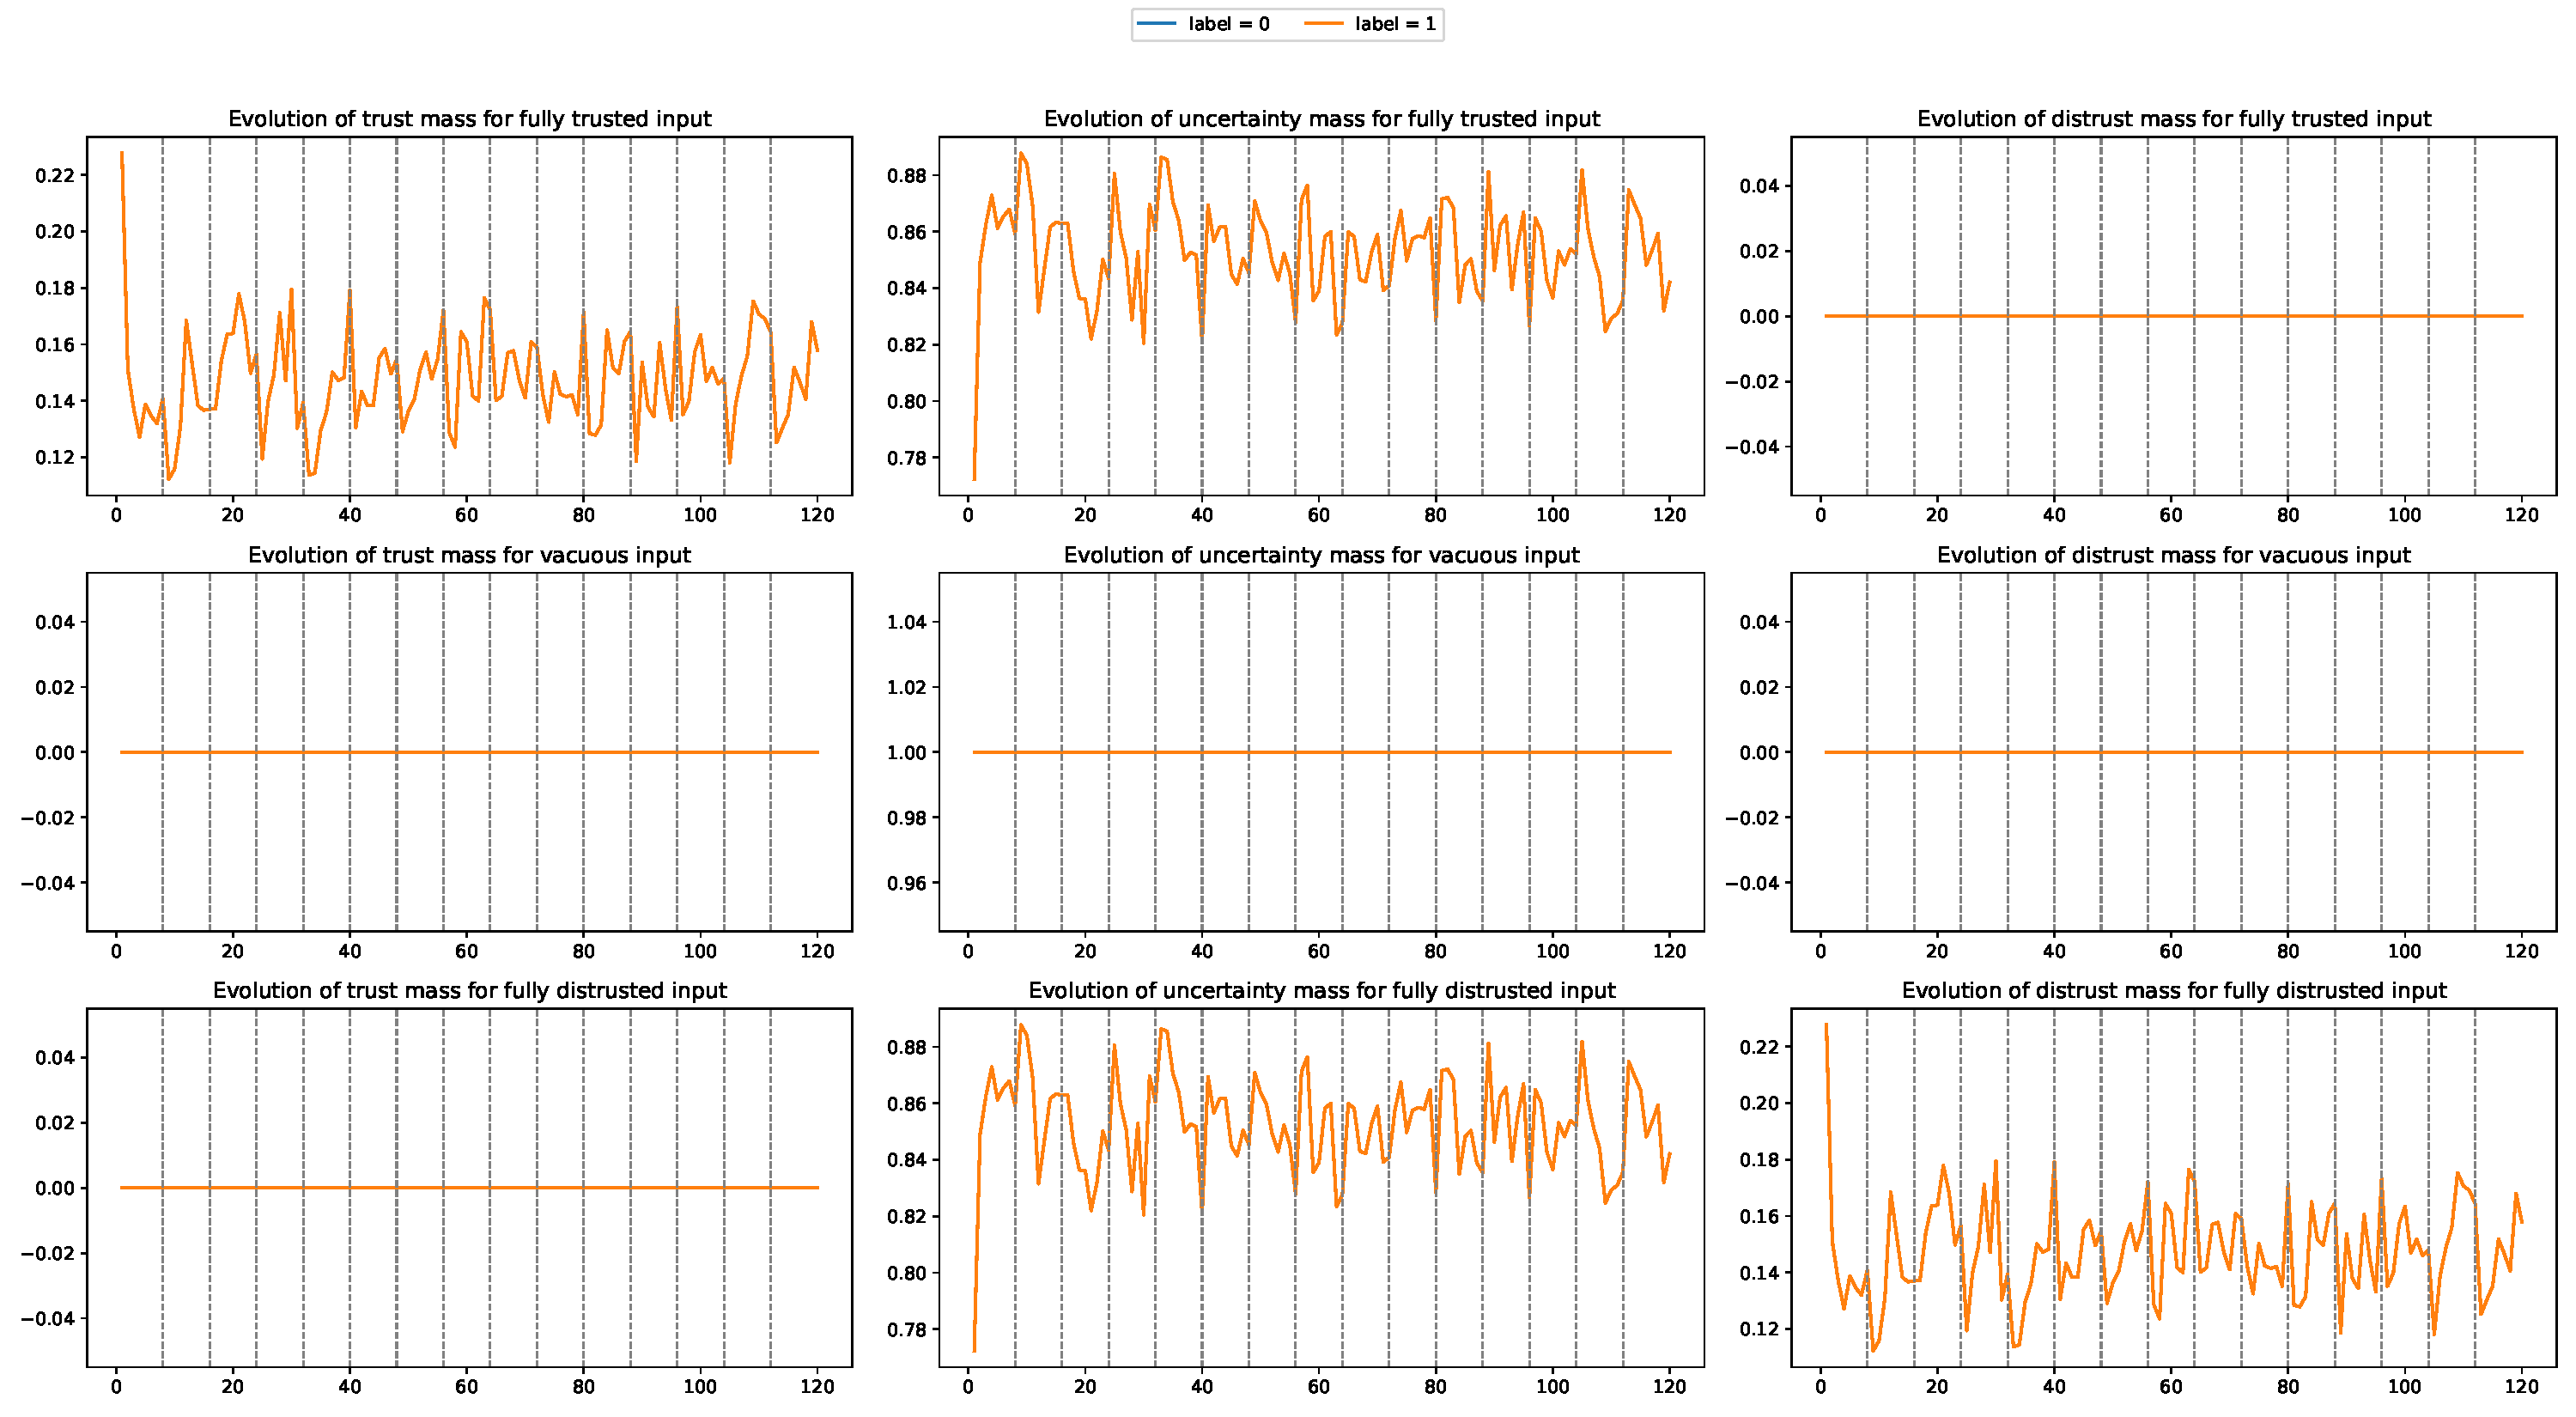
\includegraphics[width=\textwidth]{plots_v2/Cancer/eps=0.01/plot_ptas-t-v.pdf}
  \caption{Features trusted and labels vacuous}
\end{figure}
\begin{figure}[H]
  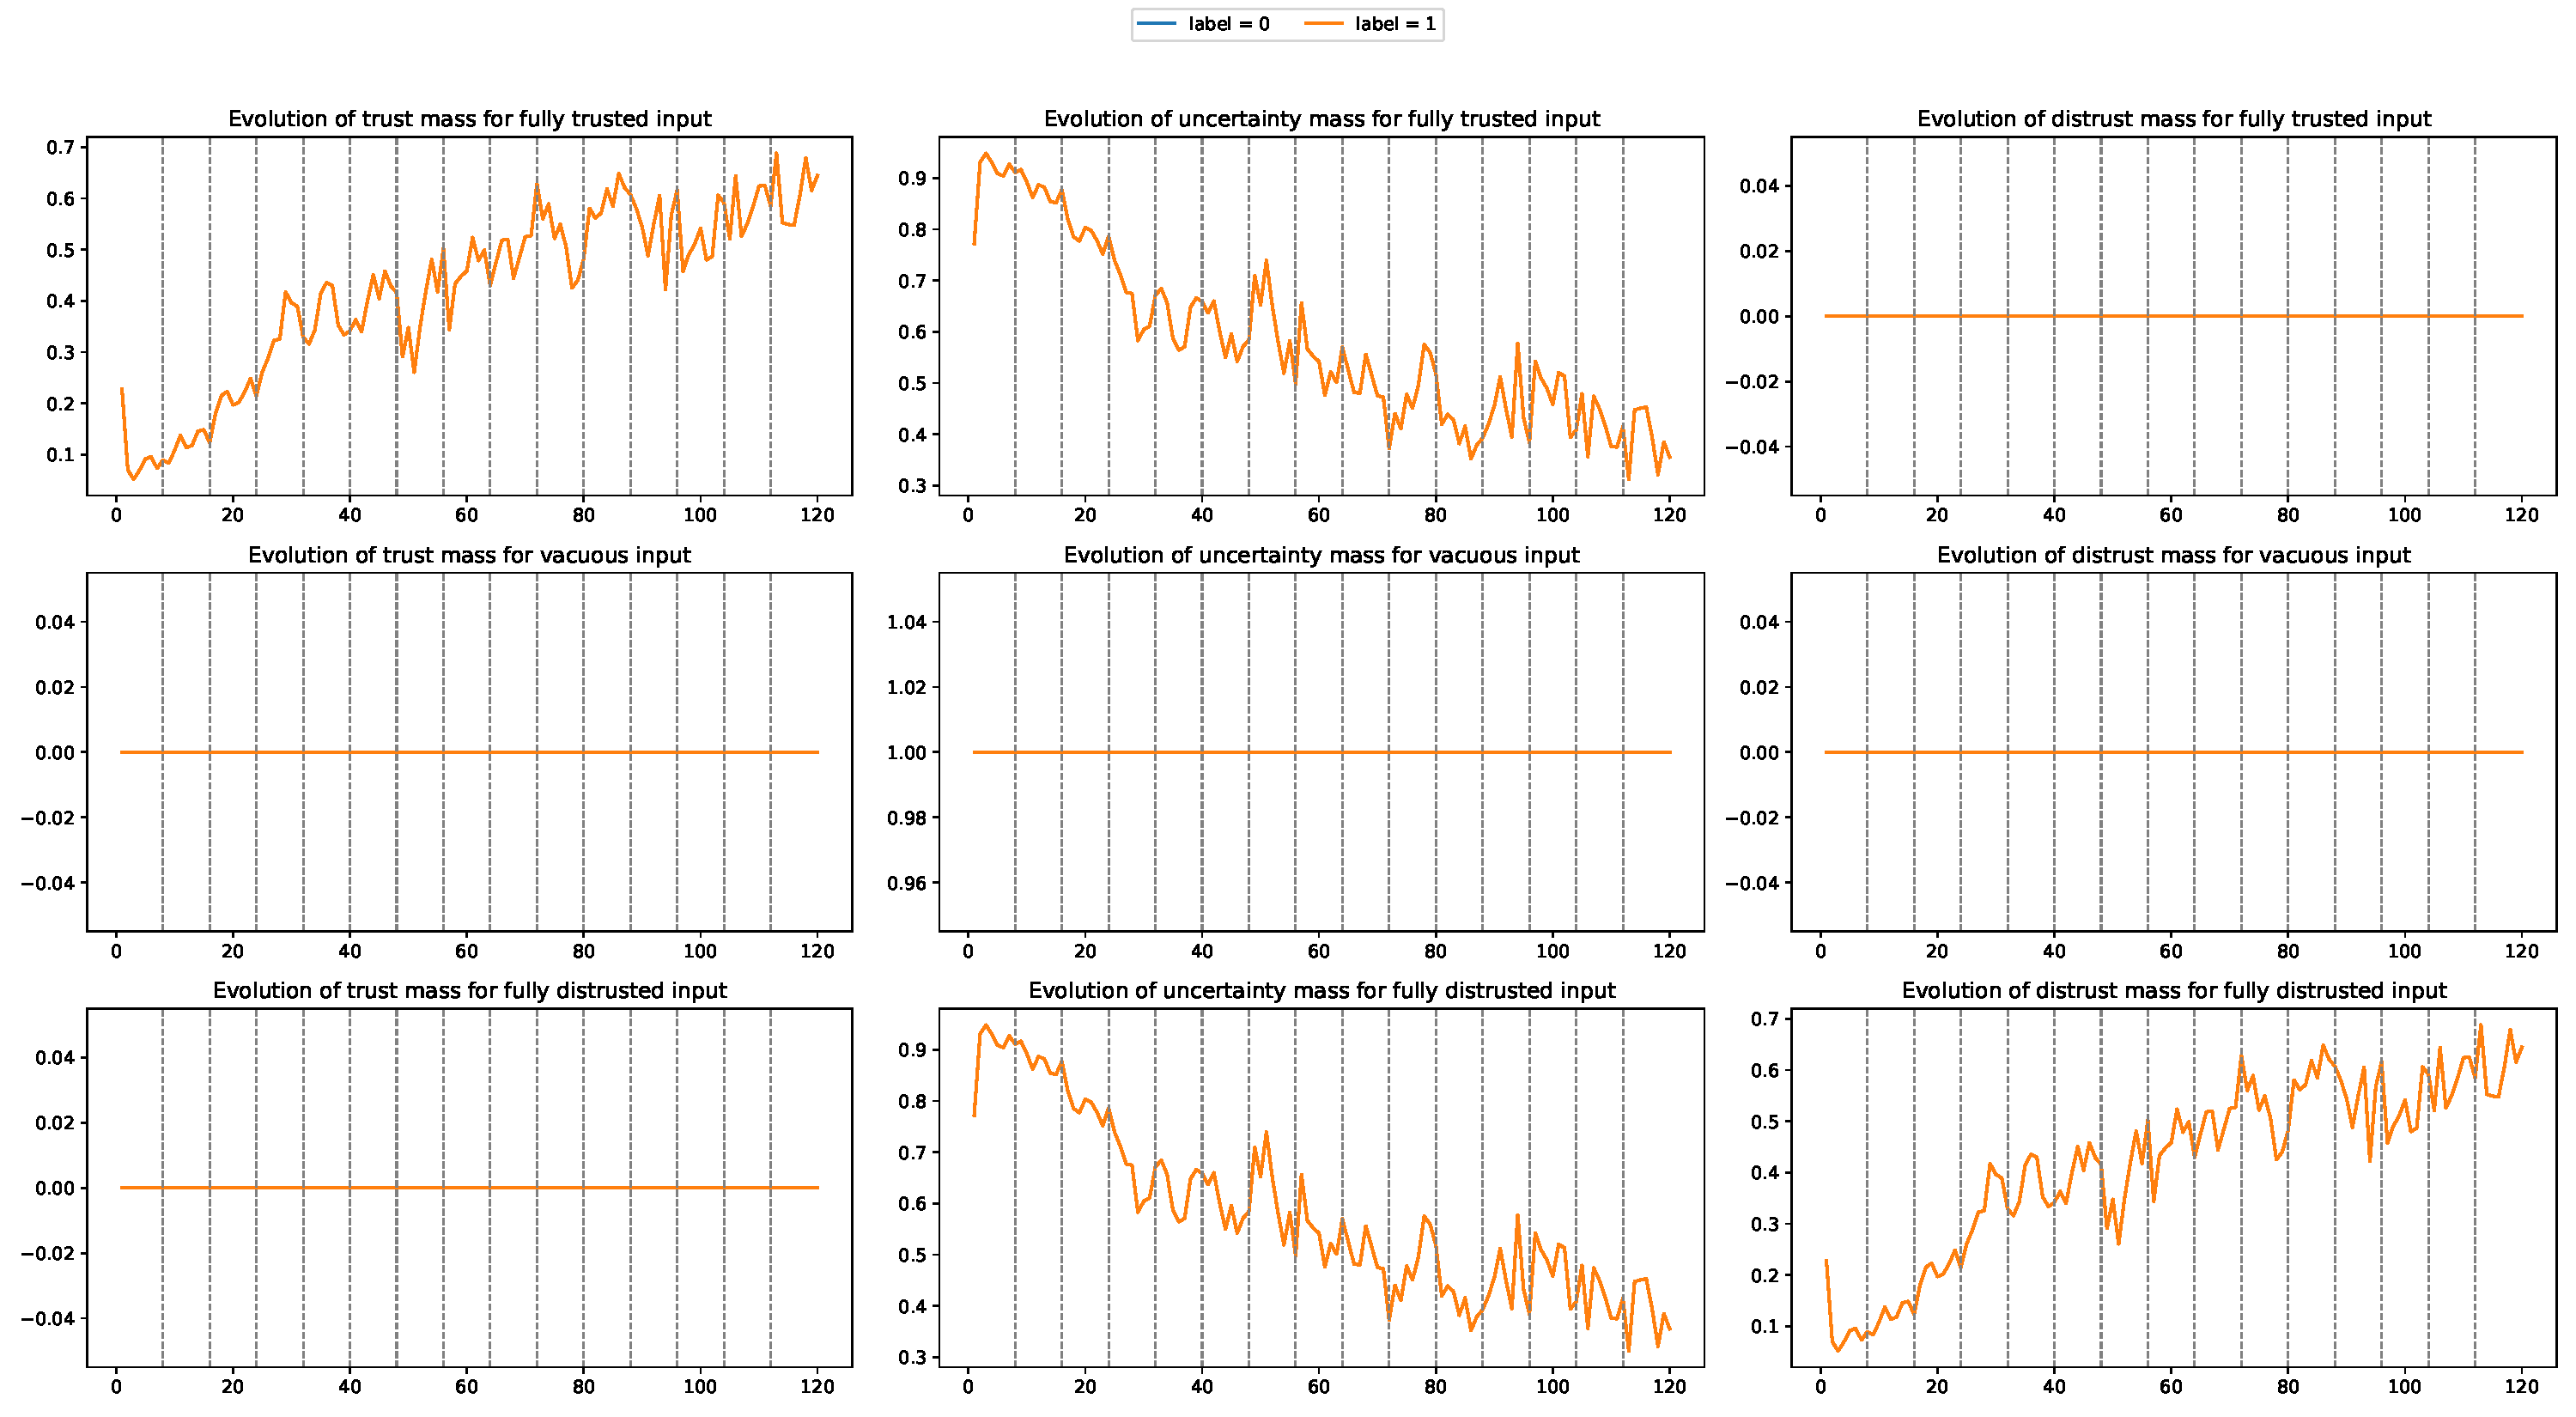
\includegraphics[width=\textwidth]{plots_v2/Cancer/eps=0.01/plot_ptas-t-t.pdf}
  \caption{Features trusted and labels trusted}
\end{figure}

\subsection{Cancer Model with \( \epsilon = 0.1 \)(\cref{exp:1})}\label{sec:rescancer0.1}
\begin{figure}[H]
  \includegraphics[width=\textwidth]{plots_v2/Cancer/eps=0.1/plot_ptas-d-d.pdf}
  \caption{Features distrusted and labels distrusted}
\end{figure}
\begin{figure}[H]
  \includegraphics[width=\textwidth]{plots_v2/Cancer/eps=0.1/plot_ptas-d-v.pdf}
  \caption{Features distrusted and labels vacuous}
\end{figure}
\begin{figure}[H]
  \includegraphics[width=\textwidth]{plots_v2/Cancer/eps=0.1/plot_ptas-d-t.pdf}
  \caption{Features distrusted and labels trusted}
\end{figure}
\begin{figure}[H]
  \includegraphics[width=\textwidth]{plots_v2/Cancer/eps=0.1/plot_ptas-v-d.pdf}
  \caption{Features vacuous and labels distrusted}
\end{figure}
\begin{figure}[H]
  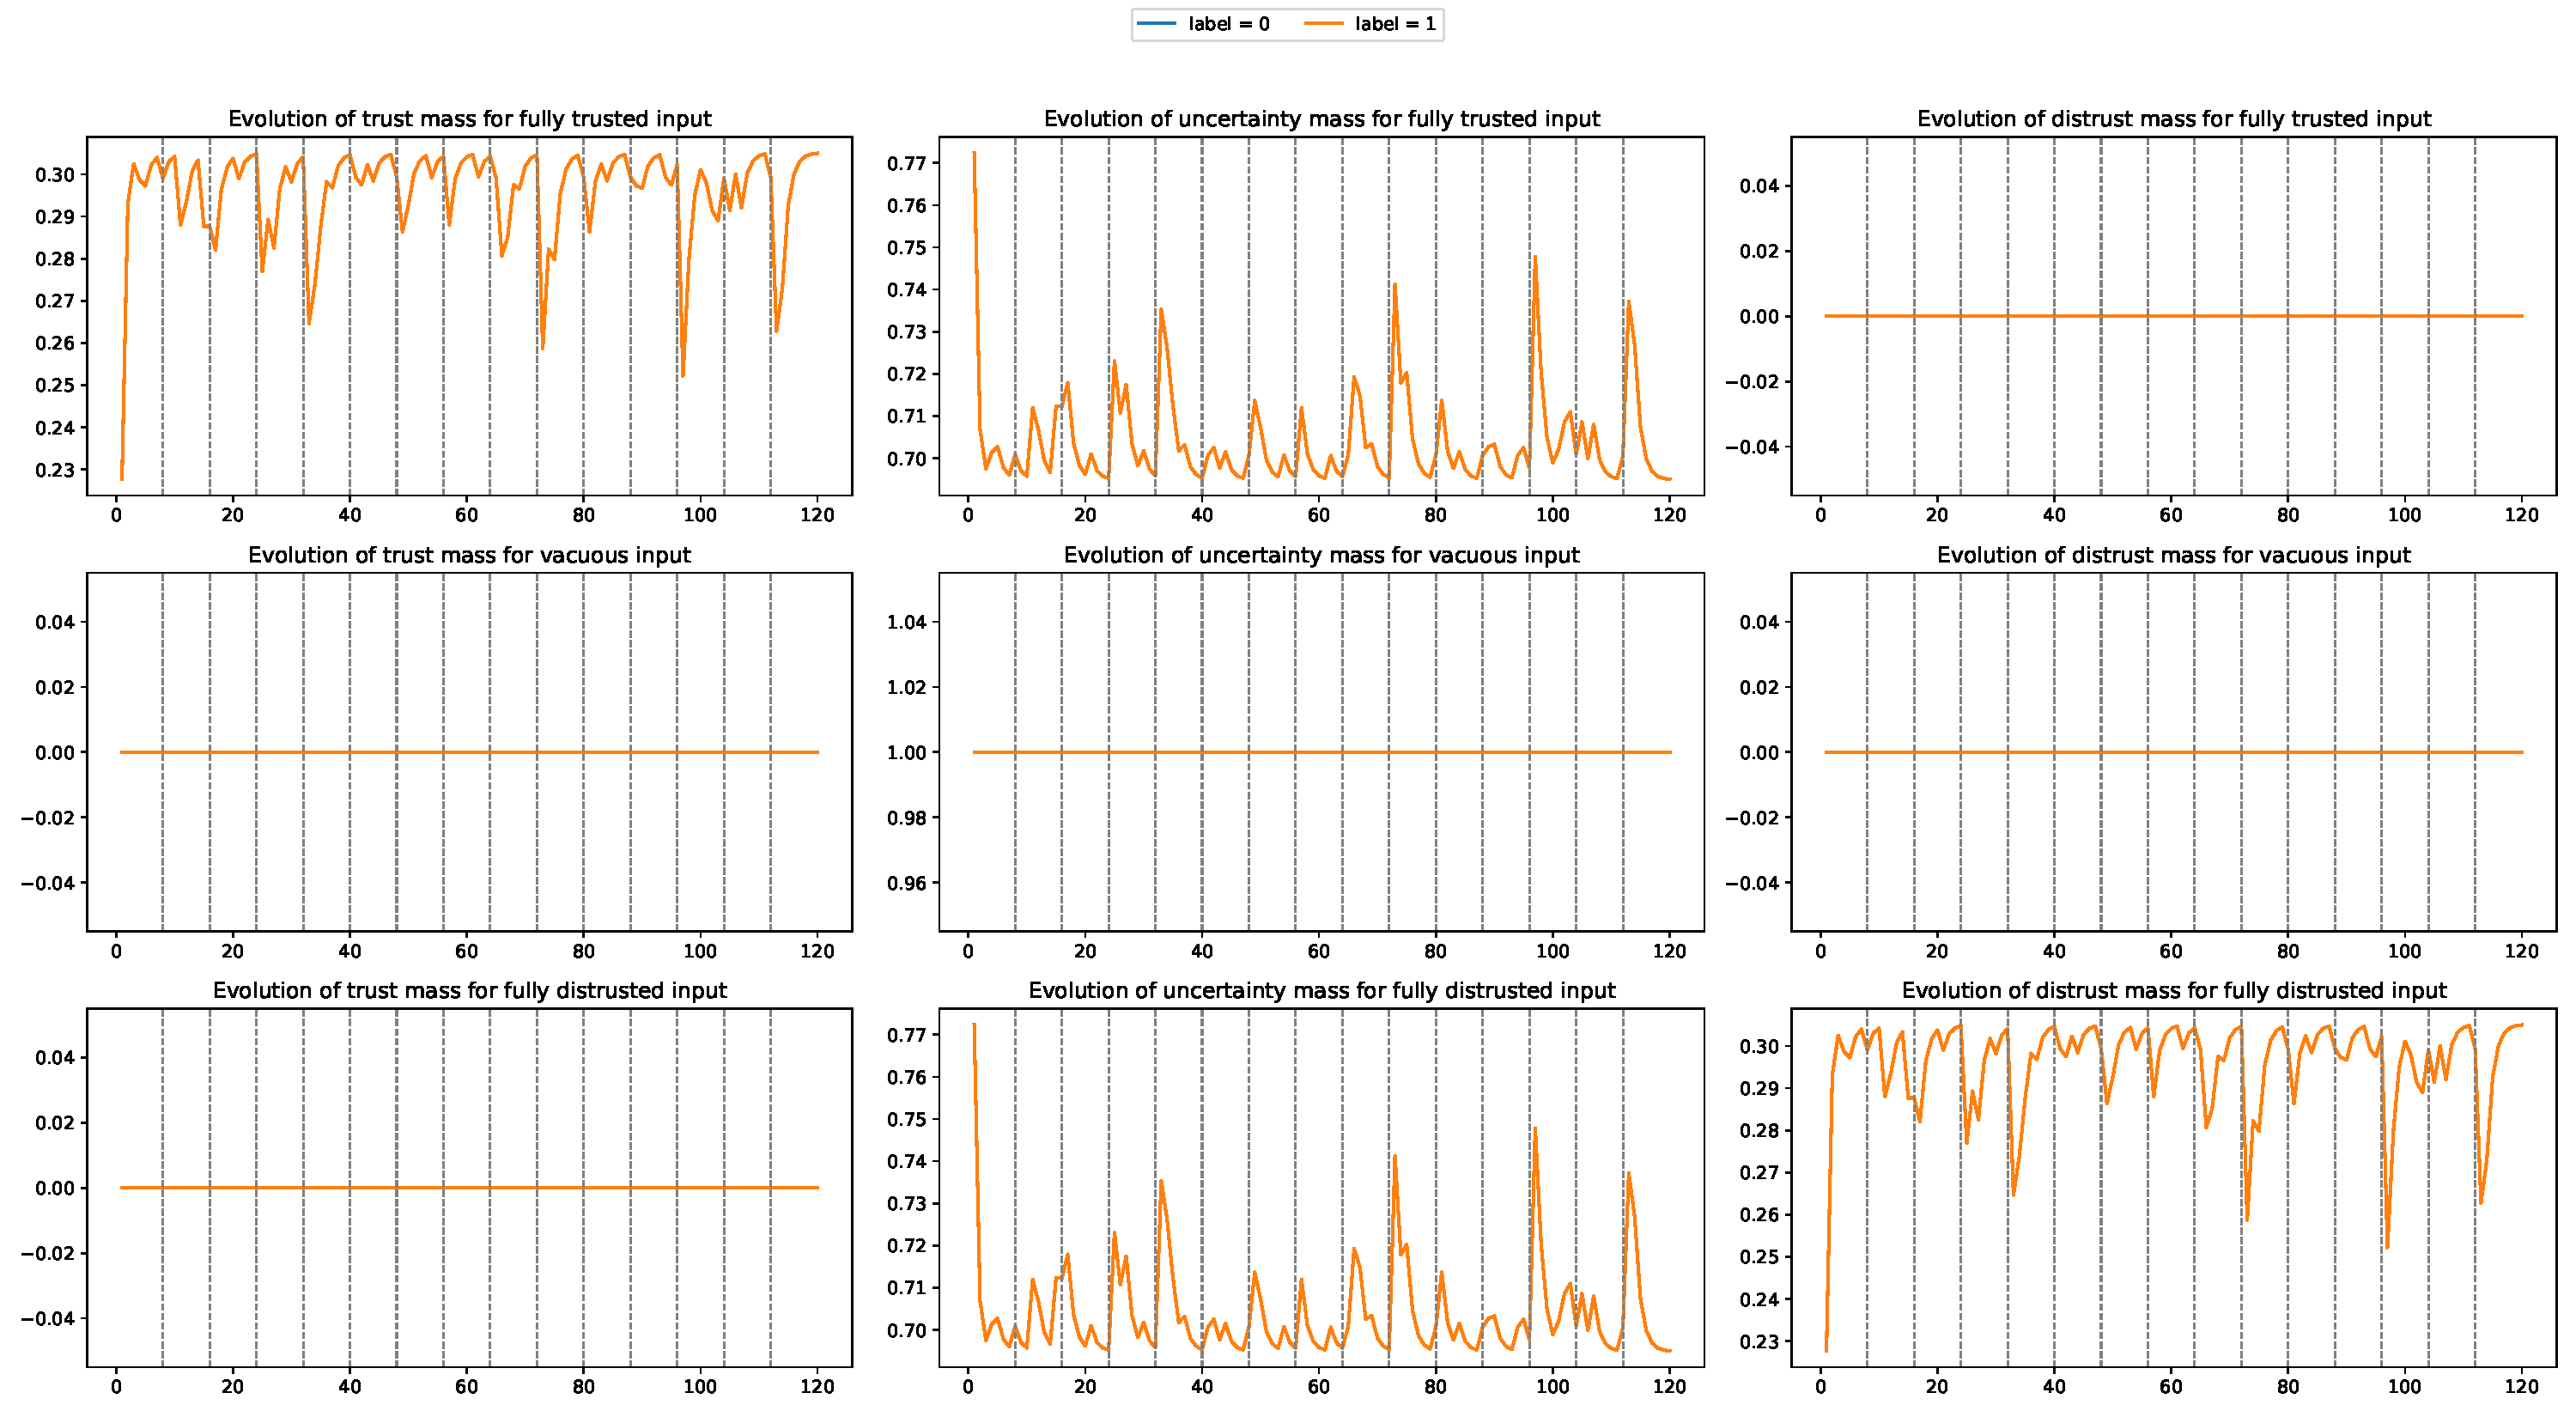
\includegraphics[width=\textwidth]{plots_v2/Cancer/eps=0.1/plot_ptas-v-v.pdf}
  \caption{Features vacuous and labels vacuous}
\end{figure}
\begin{figure}[H]
  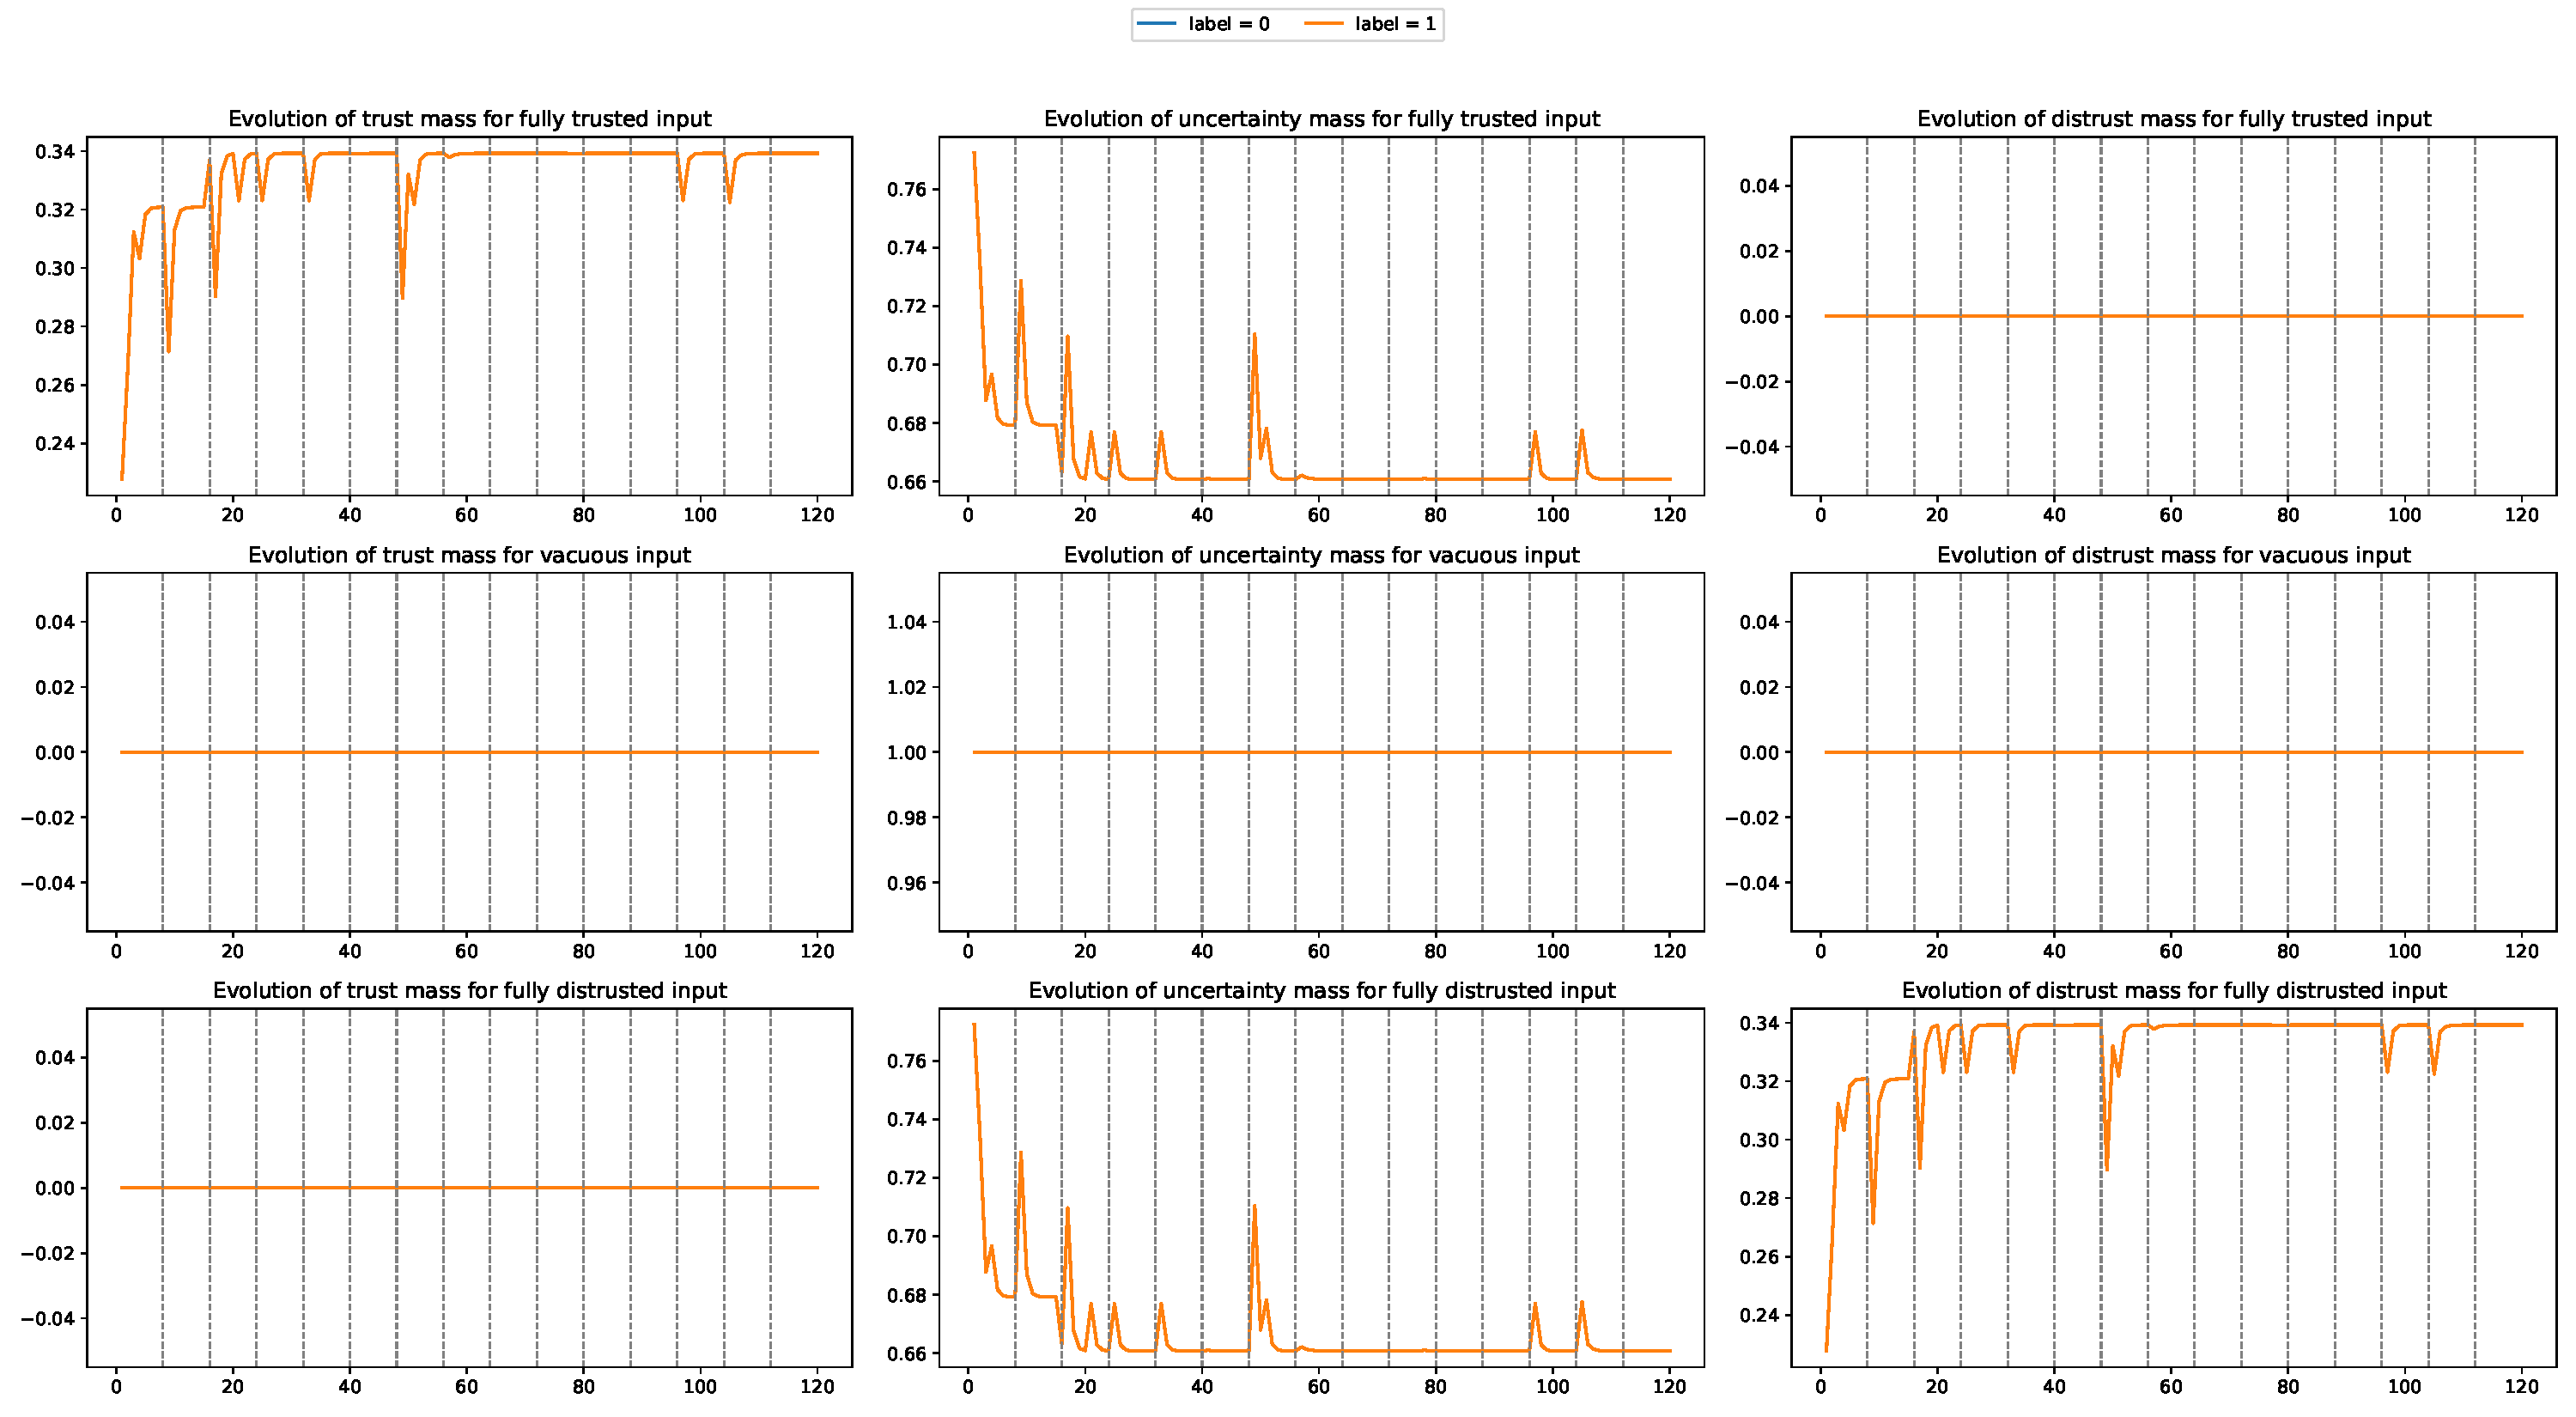
\includegraphics[width=\textwidth]{plots_v2/Cancer/eps=0.1/plot_ptas-v-t.pdf}
  \caption{Features vacuous and labels trusted}
\end{figure}
\begin{figure}[H]
  \includegraphics[width=\textwidth]{plots_v2/Cancer/eps=0.1/plot_ptas-t-d.pdf}
  \caption{Features trusted and labels distrusted}
\end{figure}
\begin{figure}[H]
  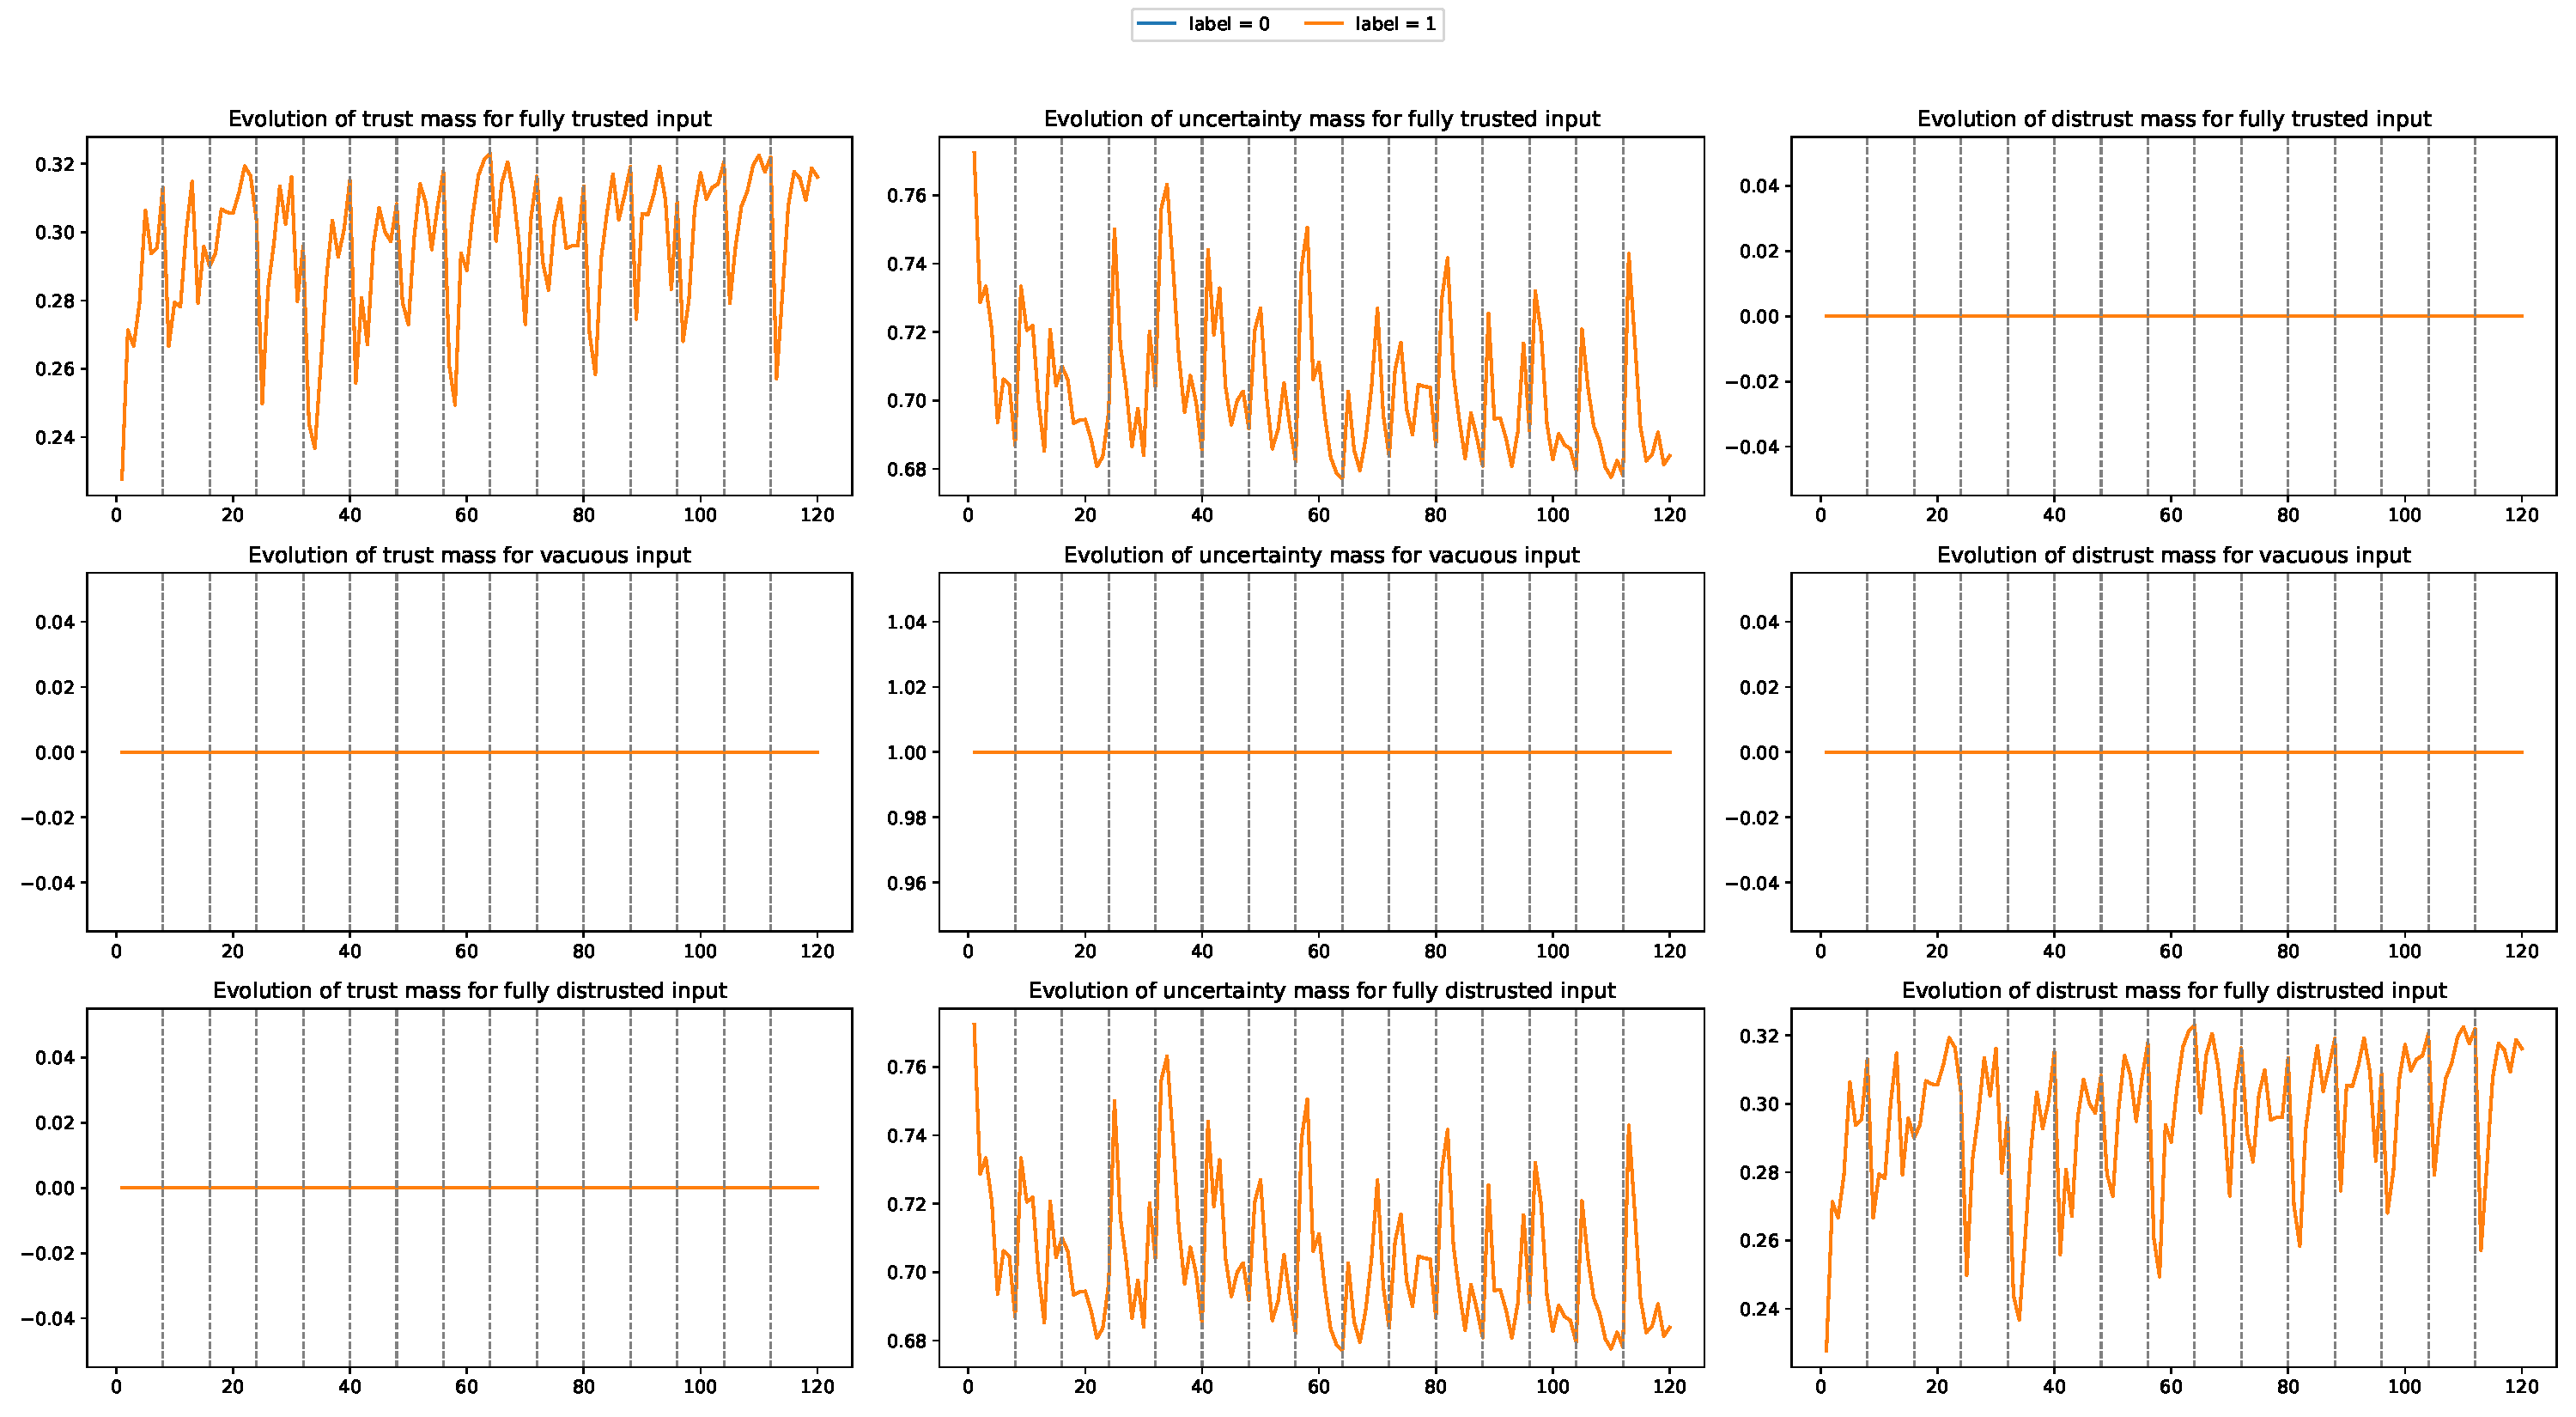
\includegraphics[width=\textwidth]{plots_v2/Cancer/eps=0.1/plot_ptas-t-v.pdf}
  \caption{Features trusted and labels vacuous}
\end{figure}
\begin{figure}[H]
  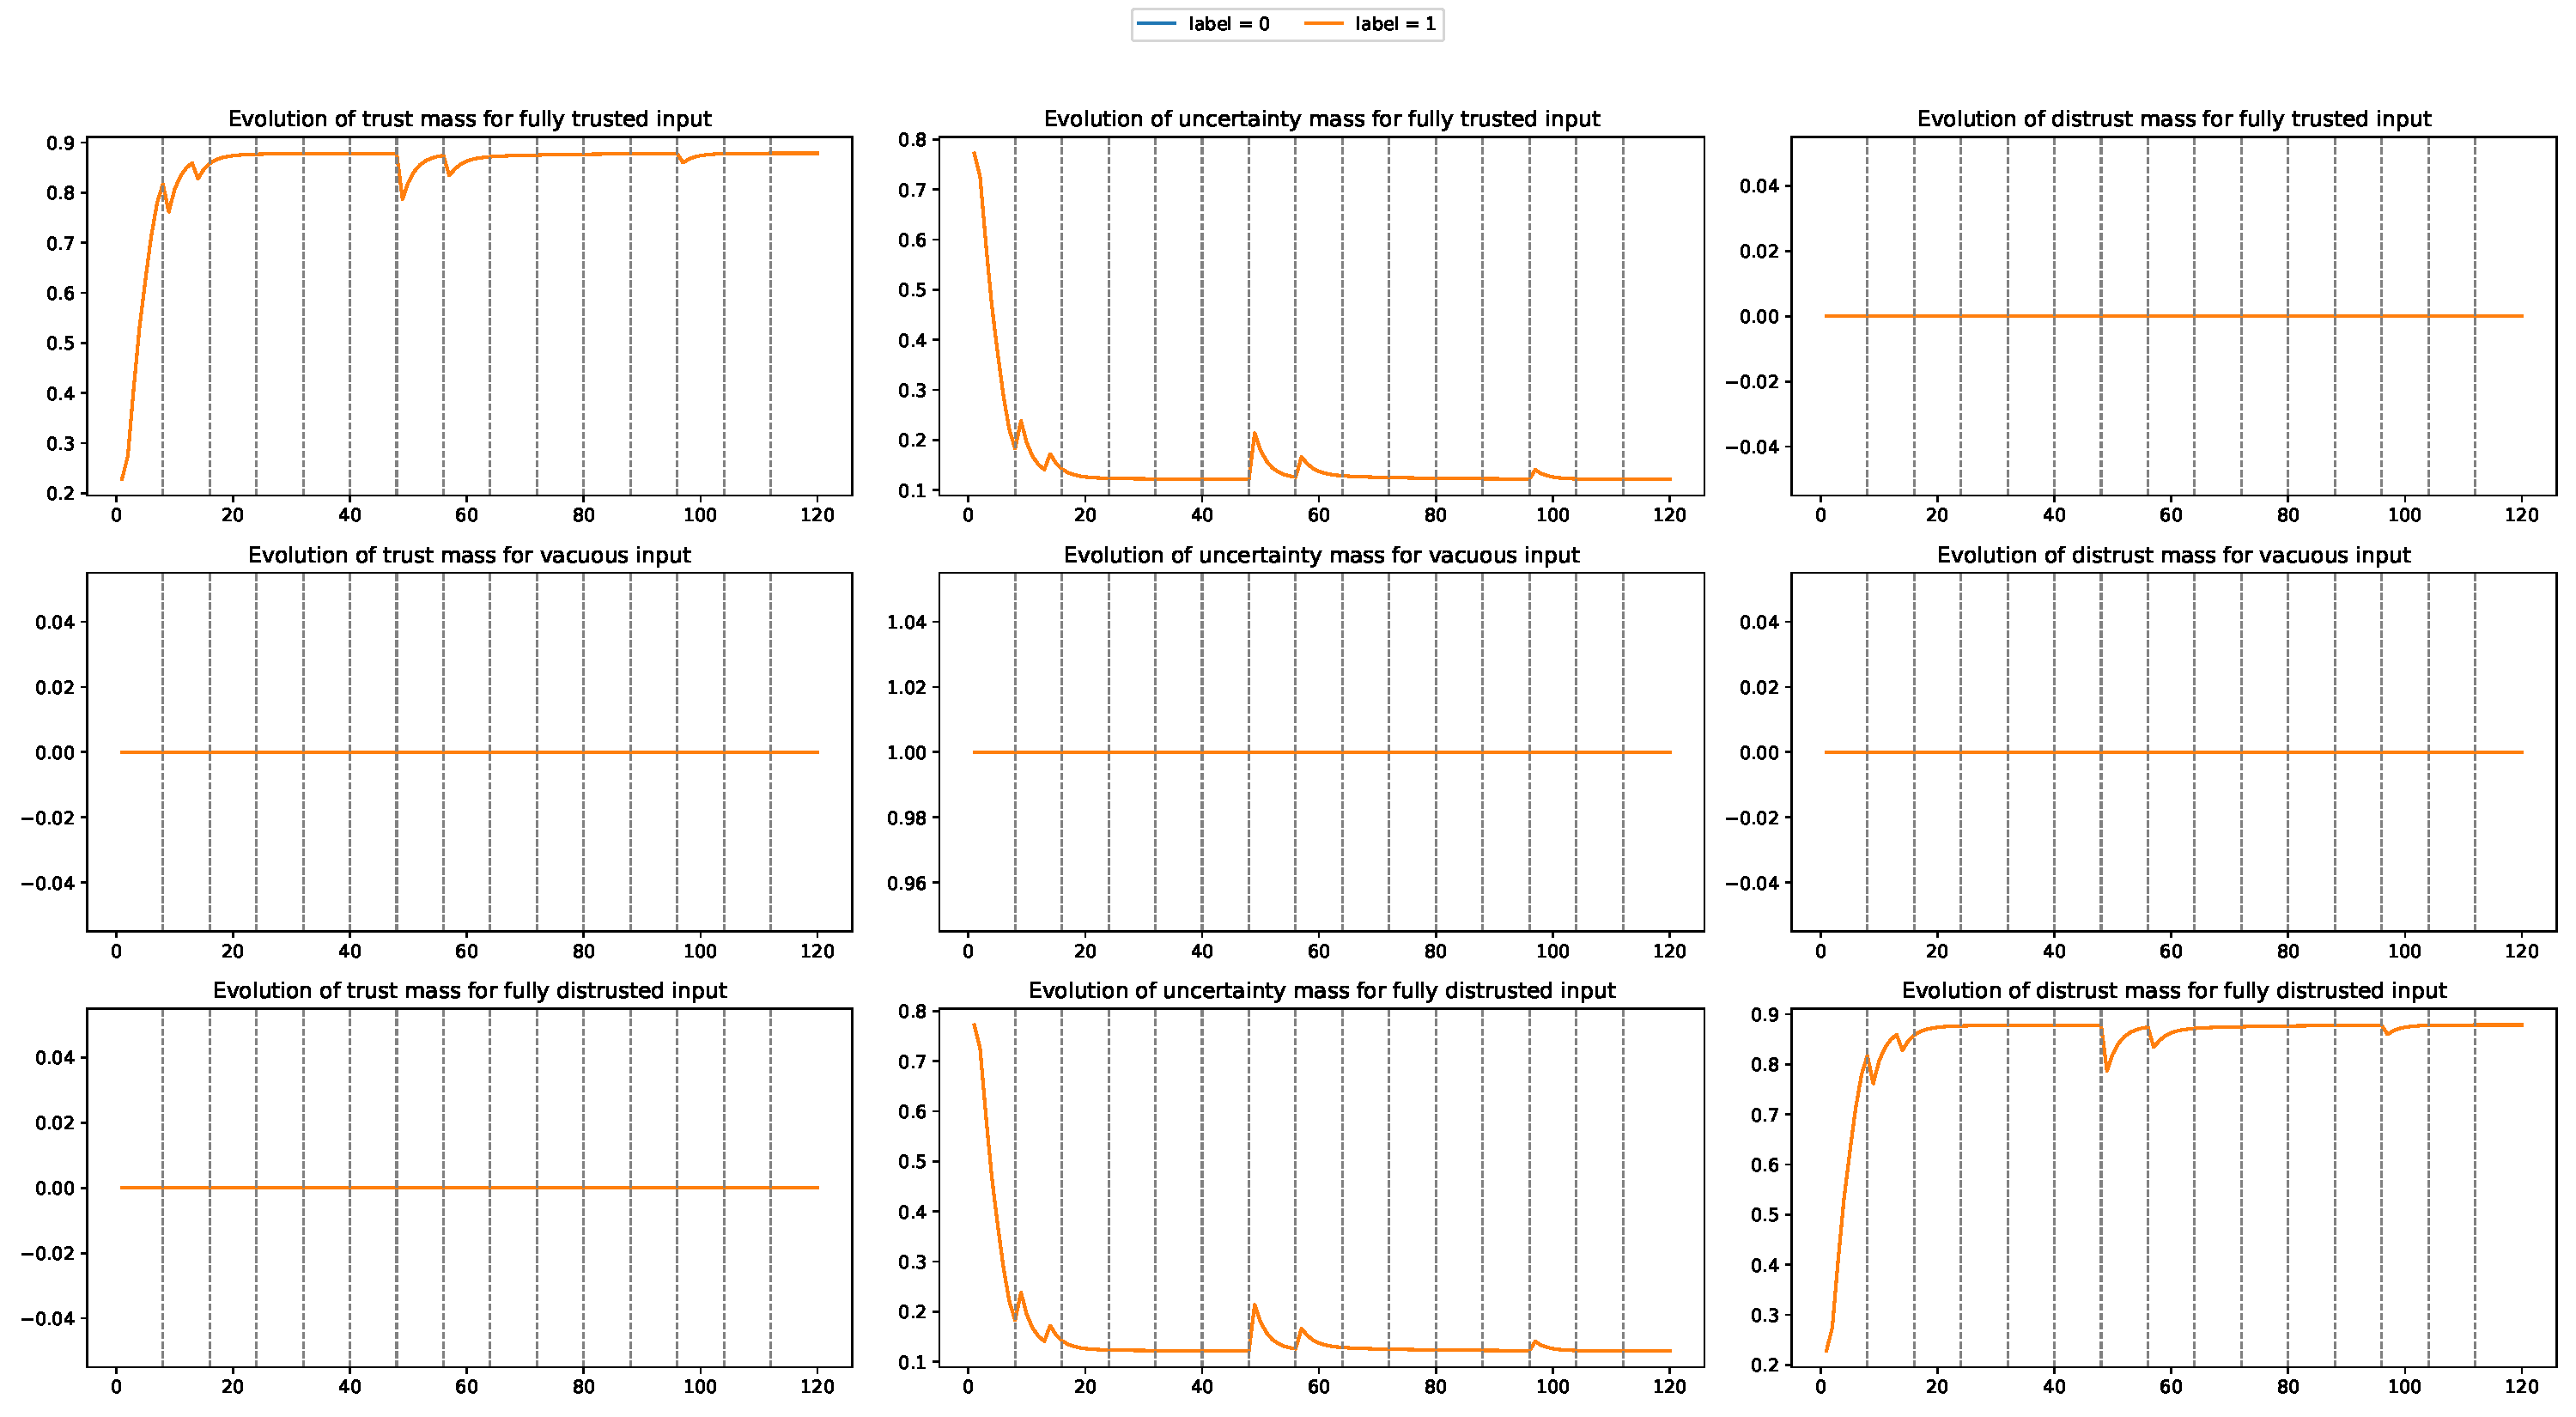
\includegraphics[width=\textwidth]{plots_v2/Cancer/eps=0.1/plot_ptas-t-t.pdf}
  \caption{Features trusted and labels trusted}
\end{figure}

\subsection{Accuracy Evolution for the Cancer Model (\cref{exp:1})}\label{sec:resmnistaccapp}
\begin{figure}[H]
\centering
\begin{subfigure}[b]{0.32\textwidth}
  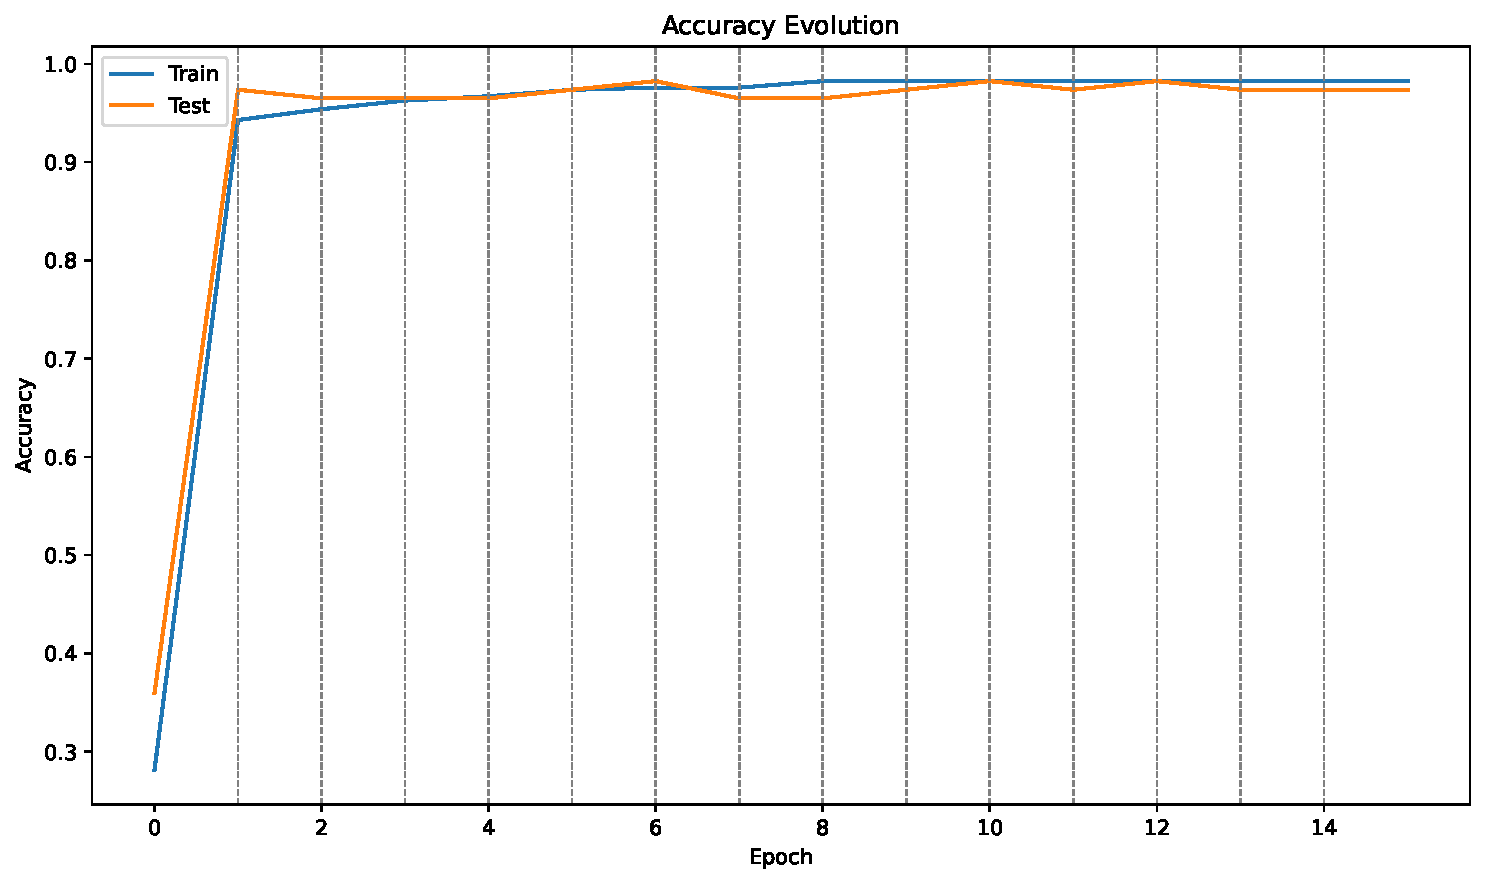
\includegraphics[width=\textwidth]{plots_v2/Cancer/eps=0.1/accuracy_evolution-t-t.pdf}
  \caption{Clean Features and Labels}
\end{subfigure}
\begin{subfigure}[b]{0.32\textwidth}
  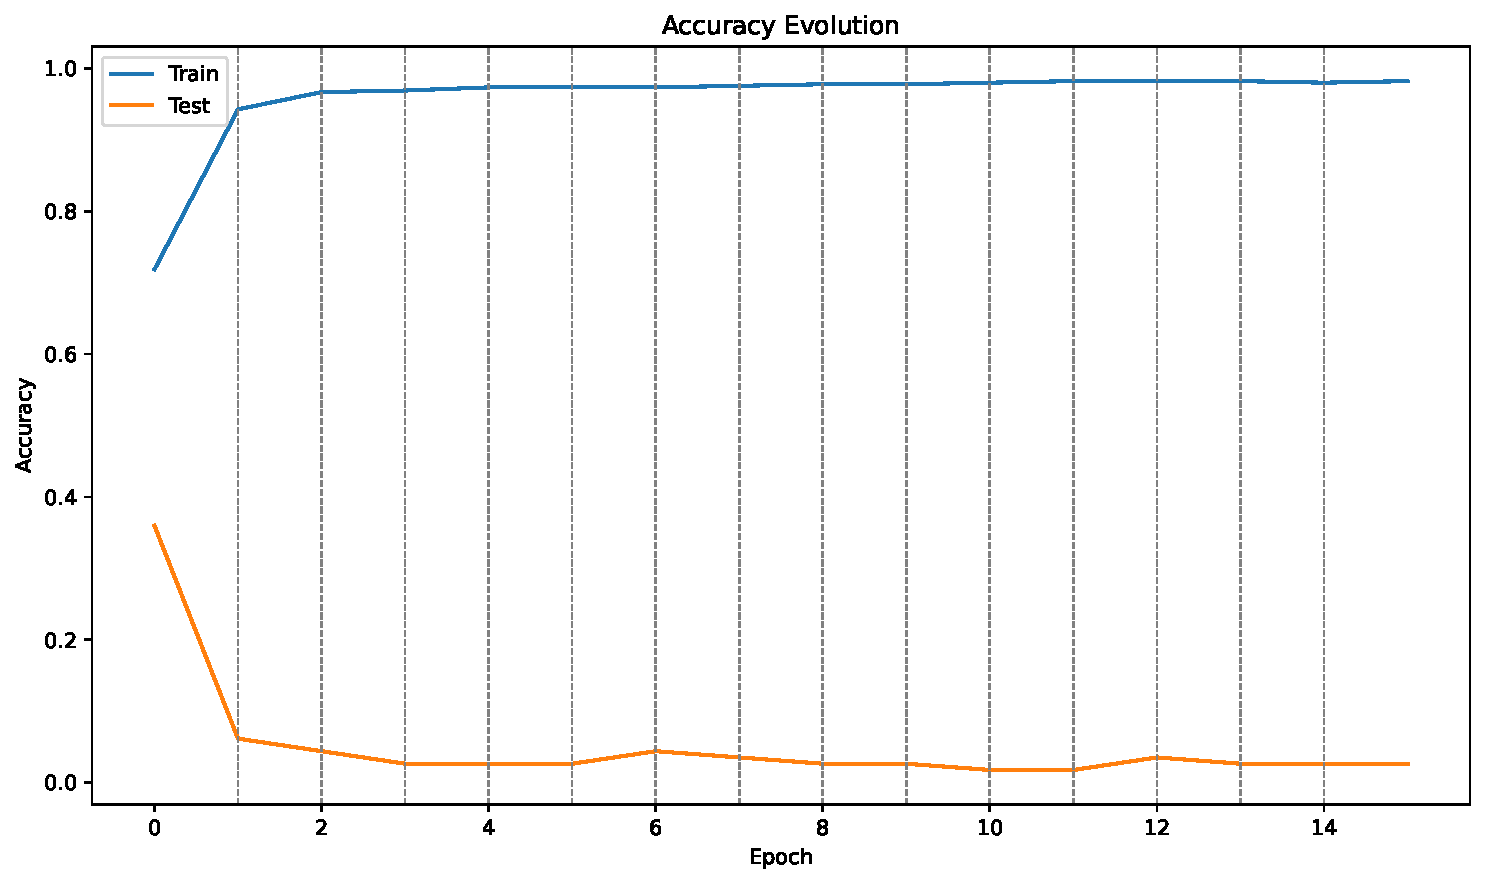
\includegraphics[width=\textwidth]{plots_v2/Cancer/eps=0.1/accuracy_evolution-t-d.pdf}
  \caption{Clean Features and Corrupted Labels}
\end{subfigure}
\begin{subfigure}[b]{0.32\textwidth}
  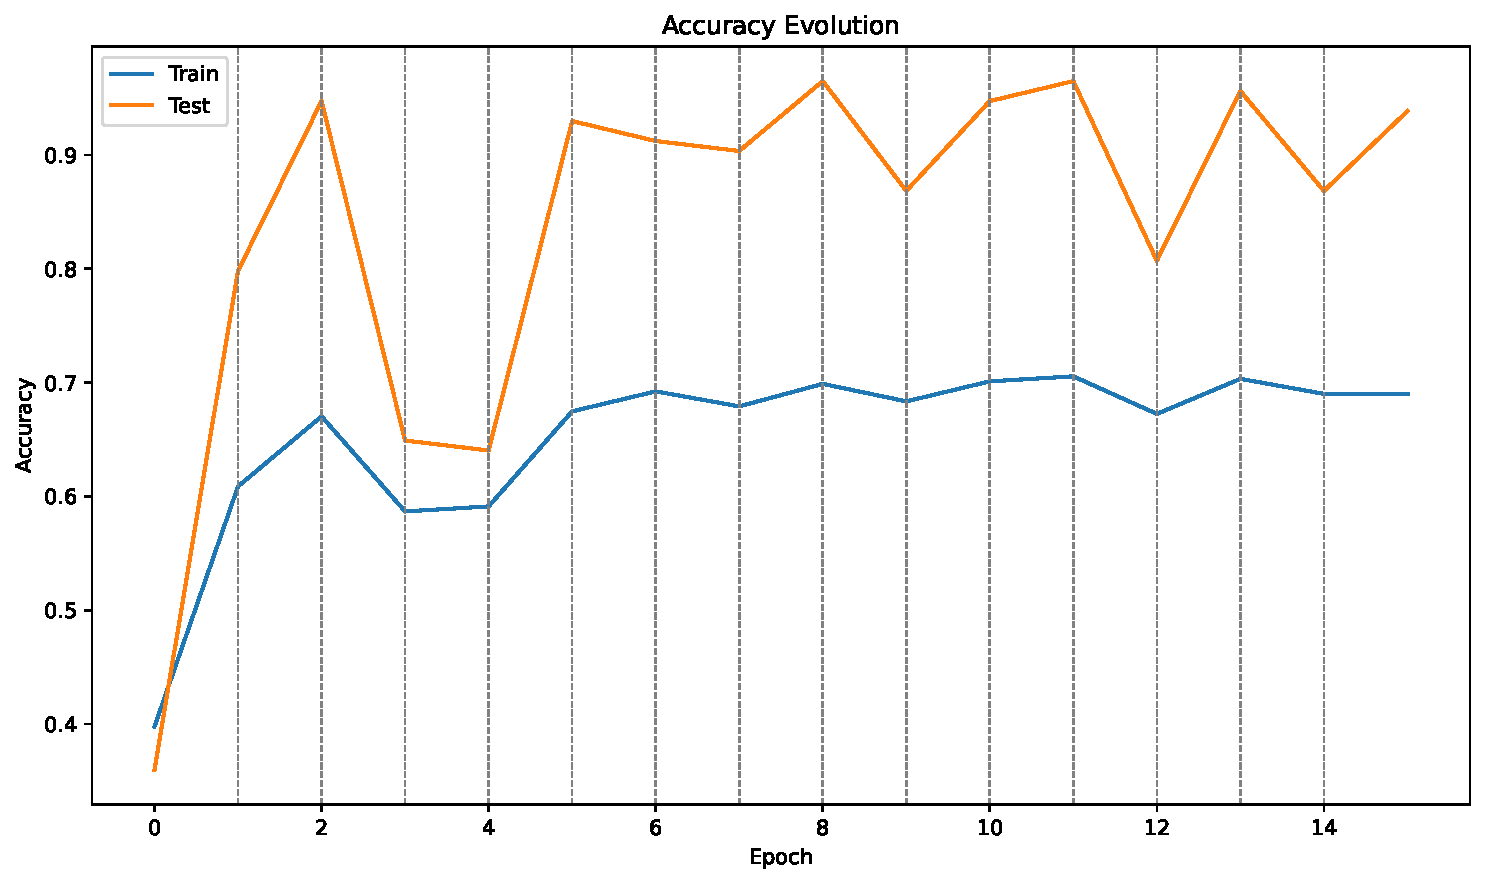
\includegraphics[width=\textwidth]{plots_v2/Cancer/eps=0.1/accuracy_evolution-t-v.pdf}
  \caption{Clean Features and Noisy Labels}
\end{subfigure}
\begin{subfigure}[b]{0.32\textwidth}
  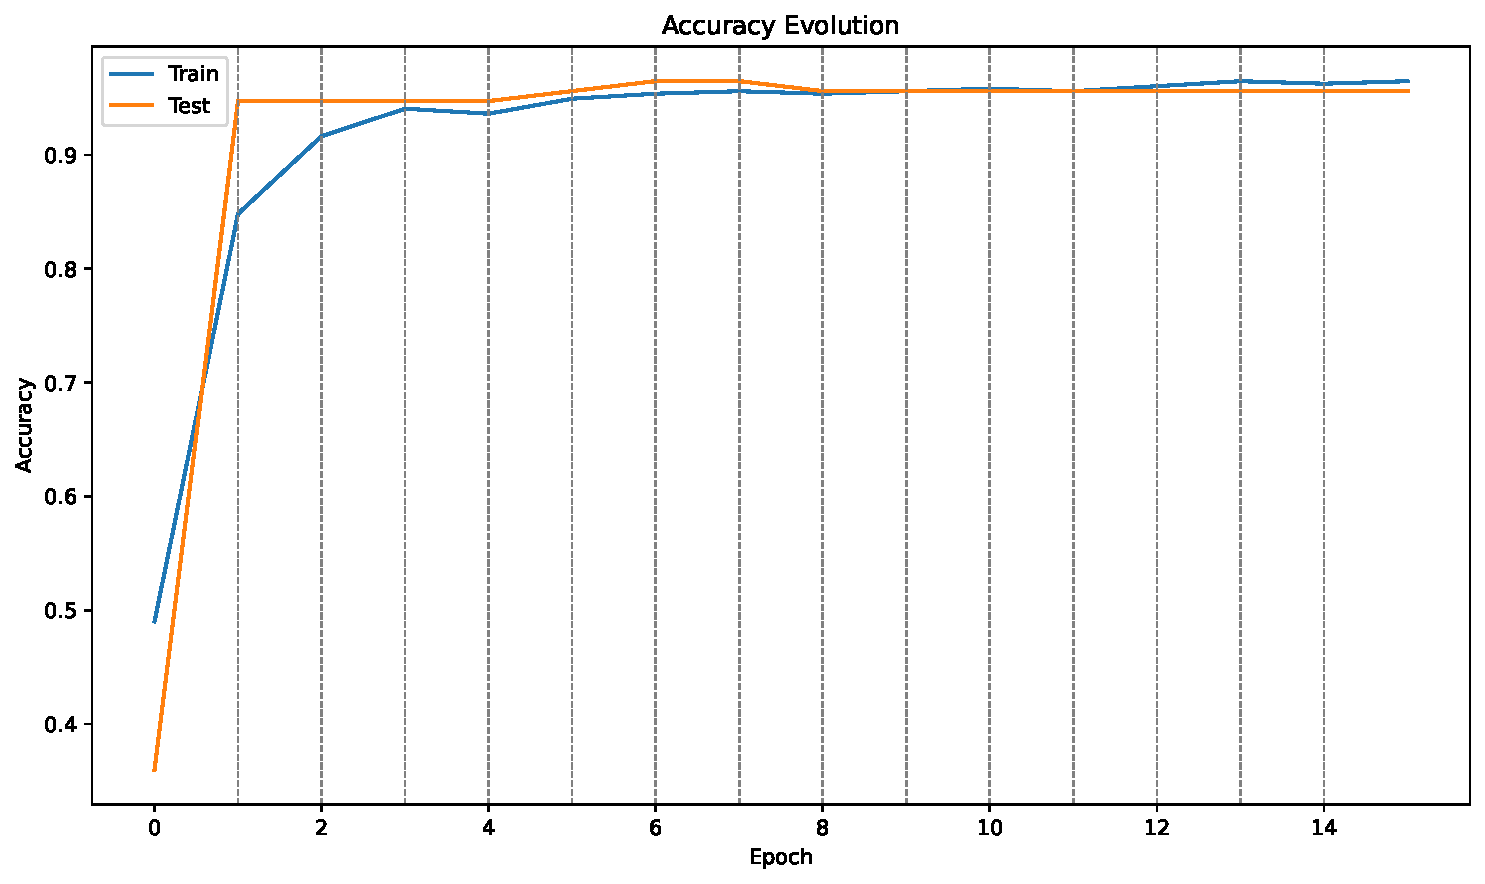
\includegraphics[width=\textwidth]{plots_v2/Cancer/eps=0.1/accuracy_evolution-v-t.pdf}
  \caption{Noisy Features and Clean Labels}
\end{subfigure}
\begin{subfigure}[b]{0.32\textwidth}
  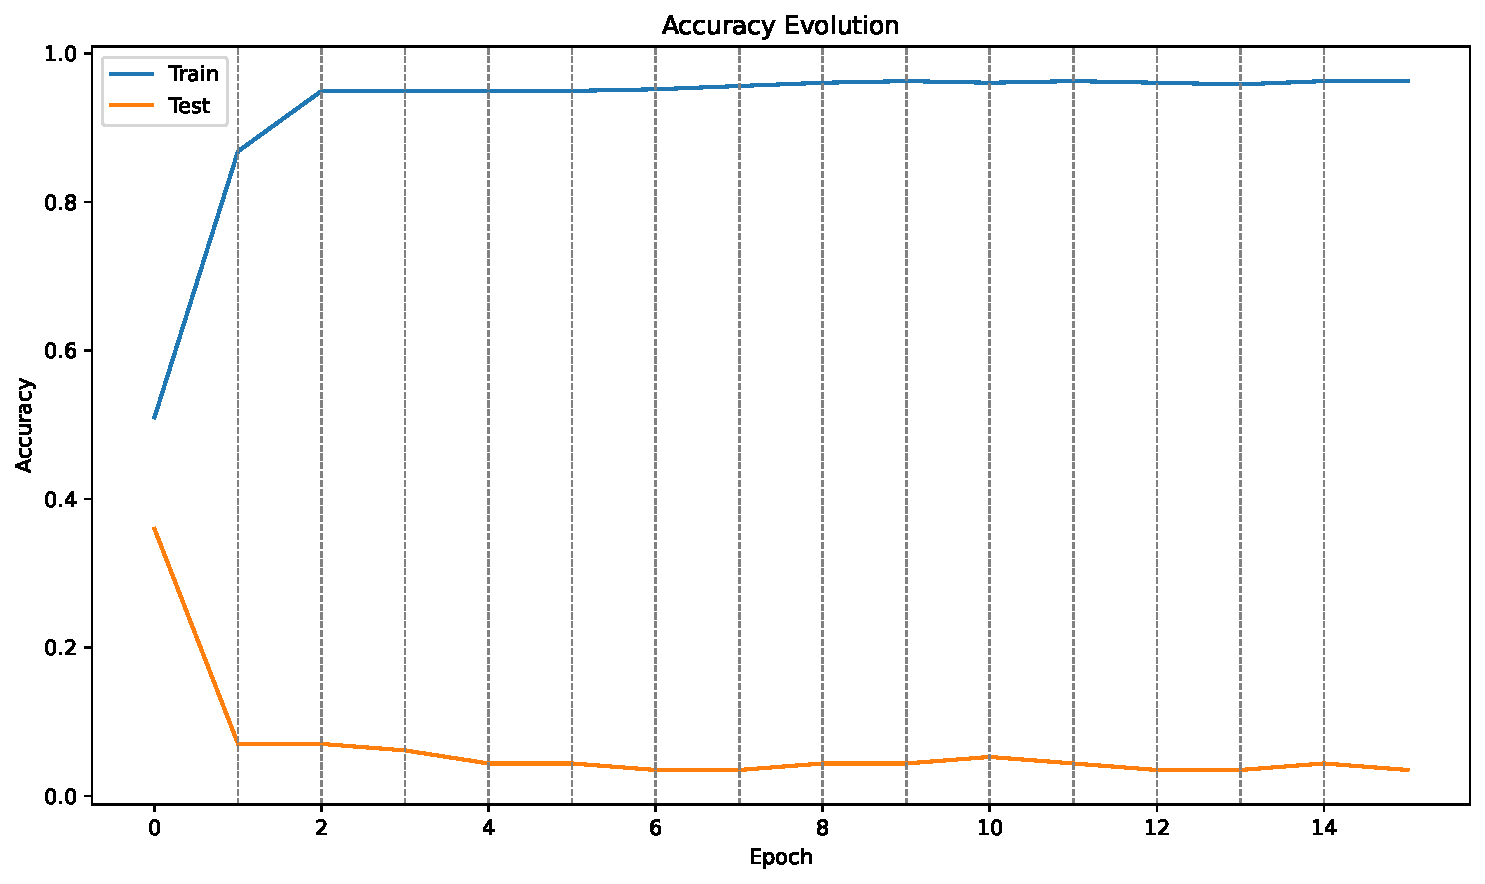
\includegraphics[width=\textwidth]{plots_v2/Cancer/eps=0.1/accuracy_evolution-v-d.pdf}
  \caption{Noisy Features and Corrupted Labels}
\end{subfigure}
\begin{subfigure}[b]{0.32\textwidth}
  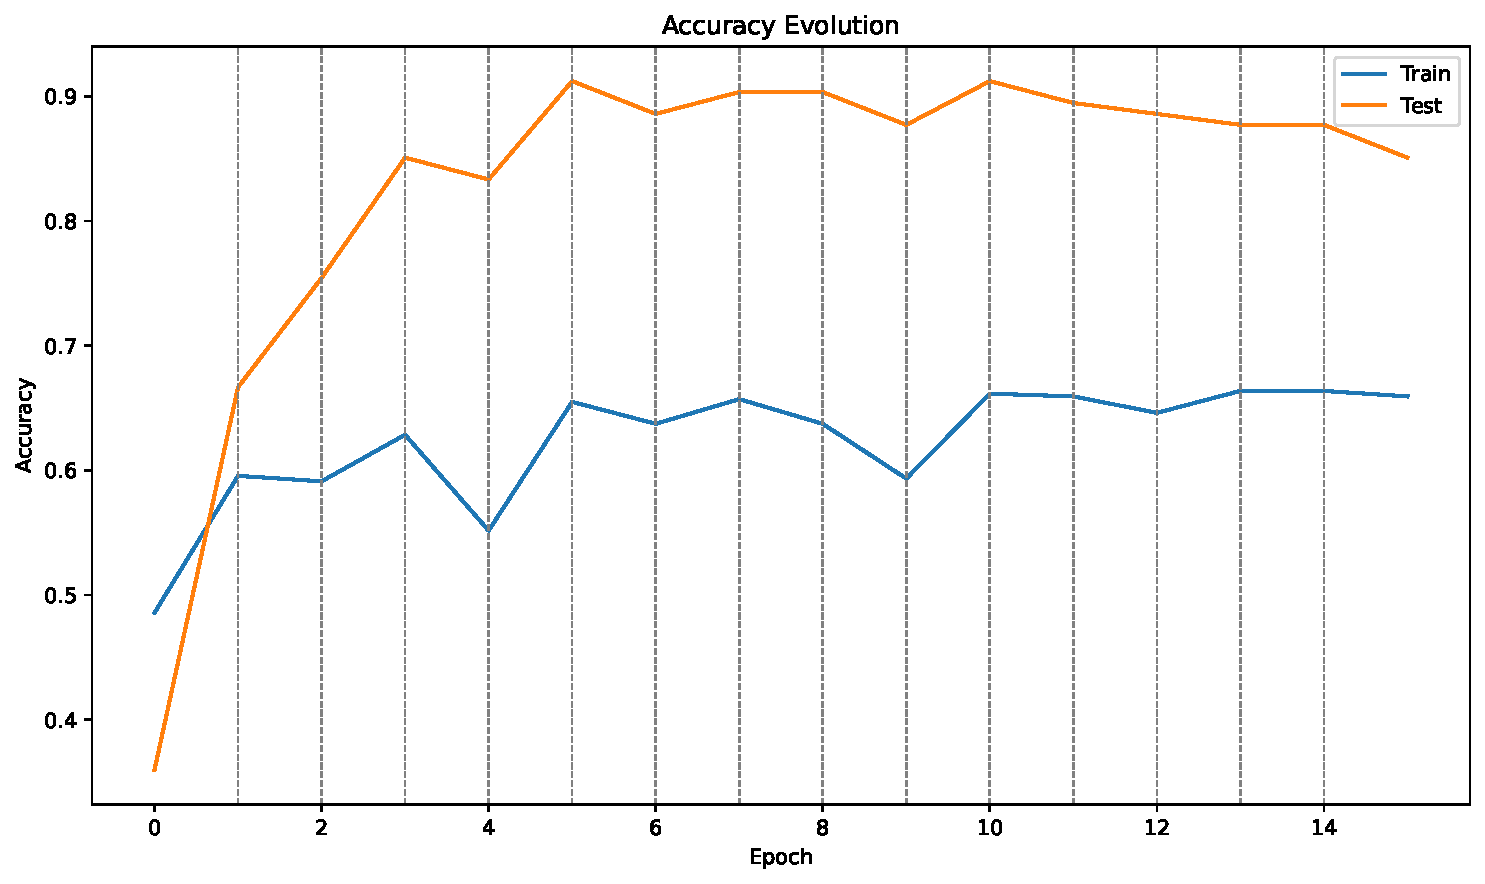
\includegraphics[width=\textwidth]{plots_v2/Cancer/eps=0.1/accuracy_evolution-v-v.pdf}
  \caption{Noisy Features and Noisy Labels}
\end{subfigure}
\begin{subfigure}[b]{0.32\textwidth}
  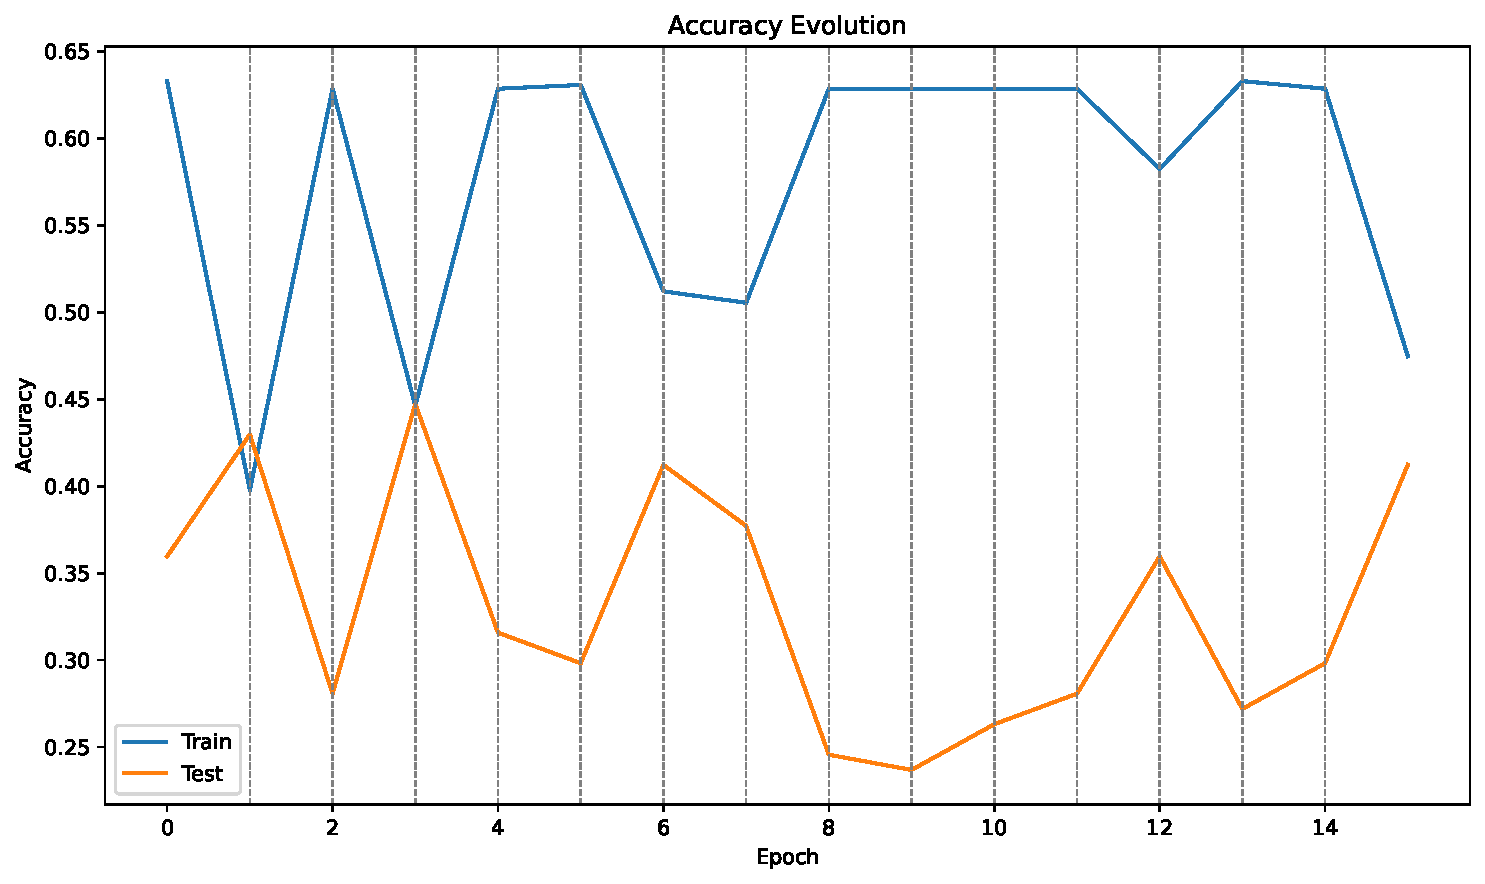
\includegraphics[width=\textwidth]{plots_v2/Cancer/eps=0.1/accuracy_evolution-d-t.pdf}
  \caption{Corrupted Features and Clean Labels}
\end{subfigure}
\begin{subfigure}[b]{0.32\textwidth}
  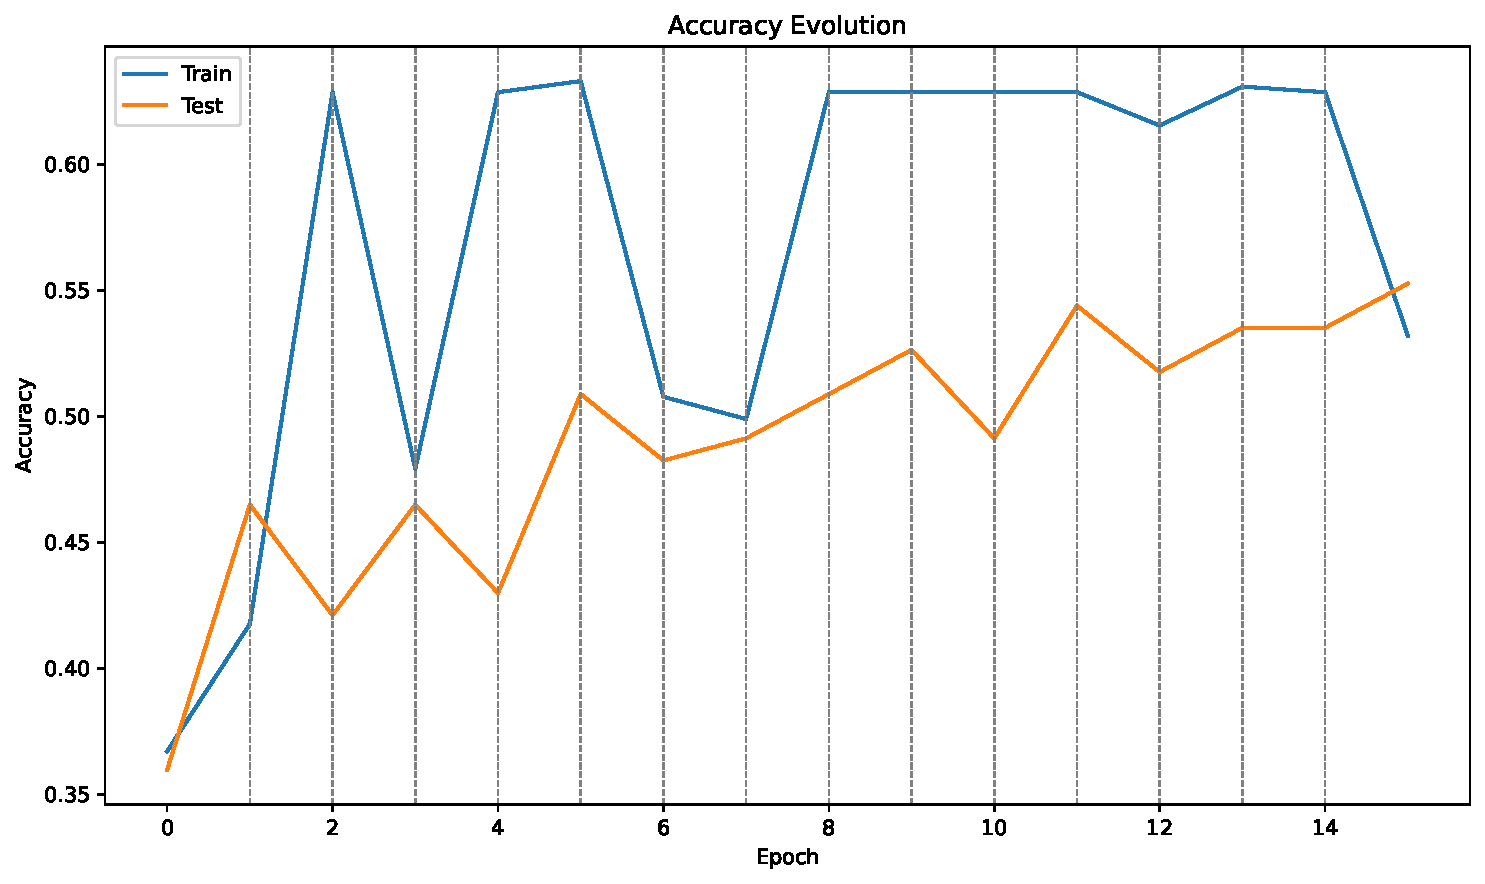
\includegraphics[width=\textwidth]{plots_v2/Cancer/eps=0.1/accuracy_evolution-d-d.pdf}
  \caption{Corrupted Features and Corrupted Labels}
\end{subfigure}
\begin{subfigure}[b]{0.32\textwidth}
  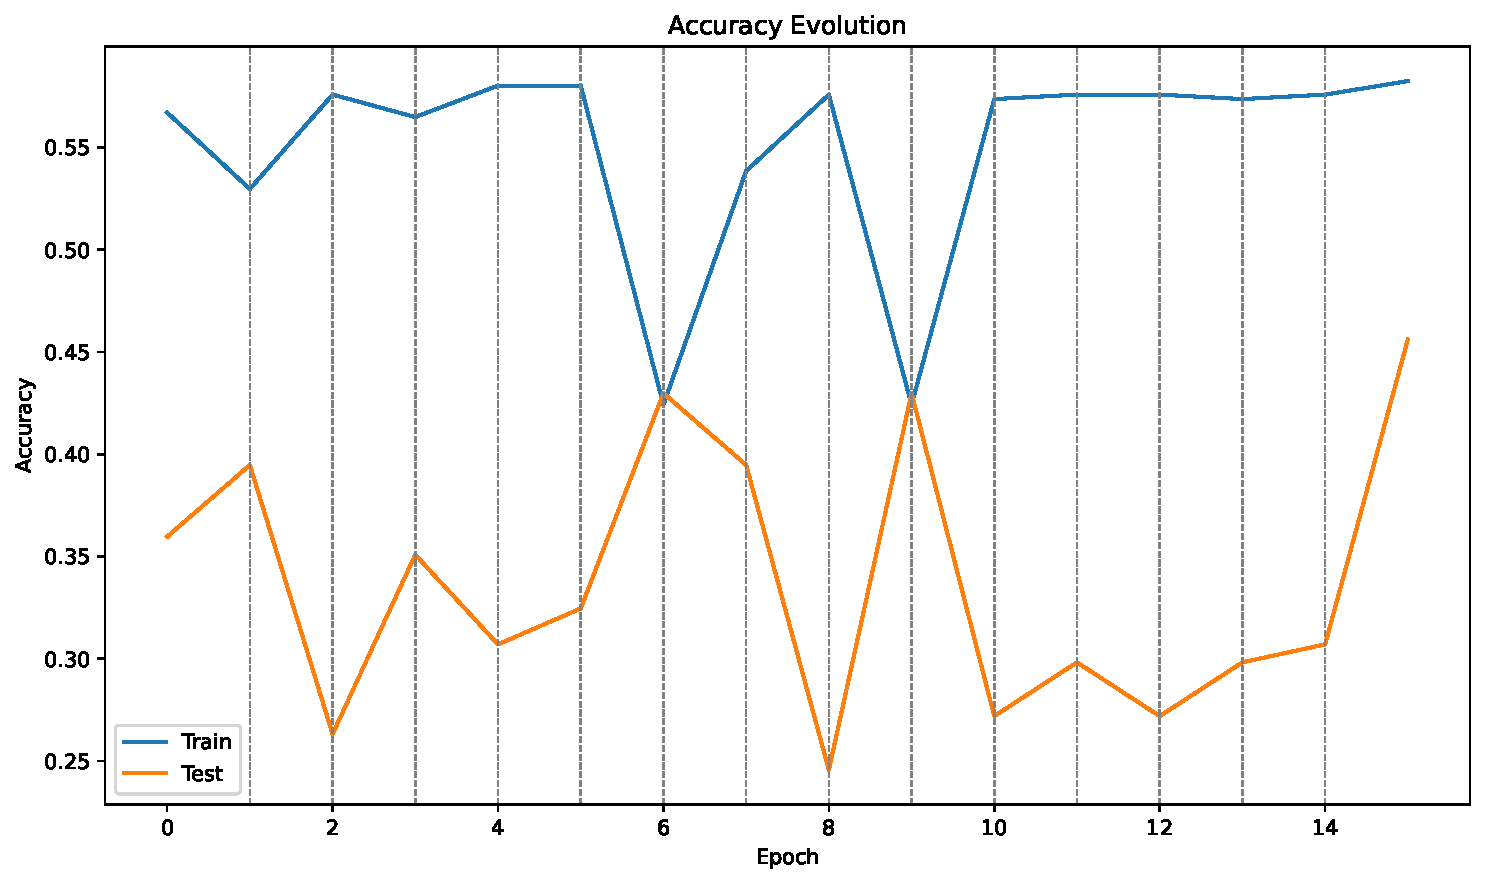
\includegraphics[width=\textwidth]{plots_v2/Cancer/eps=0.1/accuracy_evolution-d-v.pdf}
  \caption{Corrupted Features and Noisy Labels}
\end{subfigure}
\caption{Accuracy evolution of the Cancer model under different combinations of clean, corrupted, and noisy features and labels.}
\label{fig:Acccancer}
\end{figure}
% \begin{figure}[H]
%     \centering
%     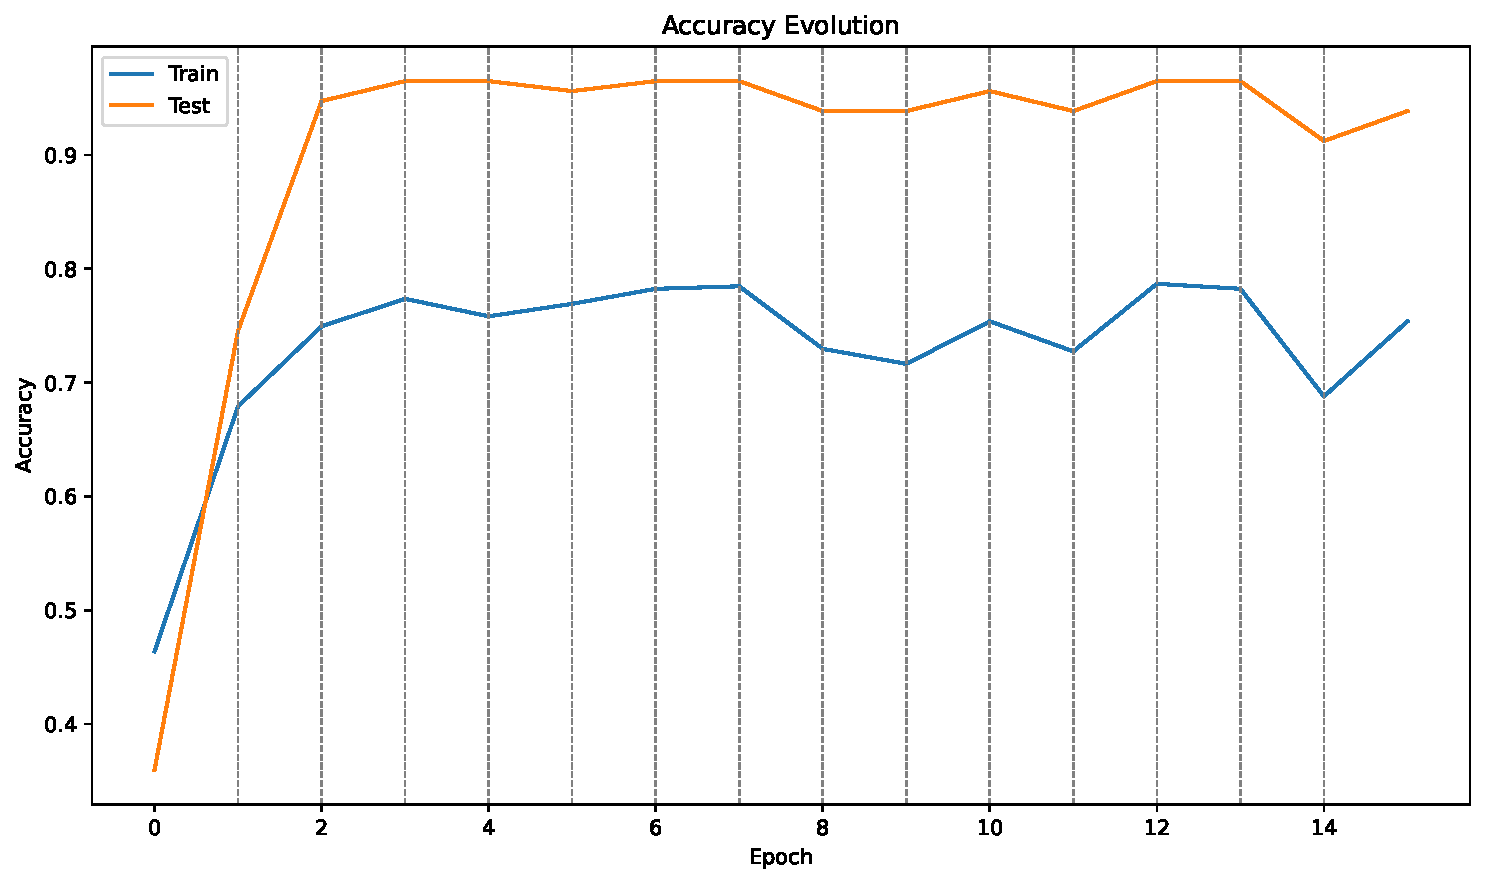
\includegraphics[width=0.8\linewidth]{good_plots/accuracy/Cancer/0.15-0.25/Cancer-noise-noise.pdf}
%     \caption{Accuracy evolution of the Cancer model when reducing the noise for noised features and labels.}
%     \label{fig:AcccancerInt}
% \end{figure}

\subsection{MNIST with Vacuous Trust Assessment (\cref{exp:2})}\label{sec:resmnist}
\begin{figure}[H]
  \centering
  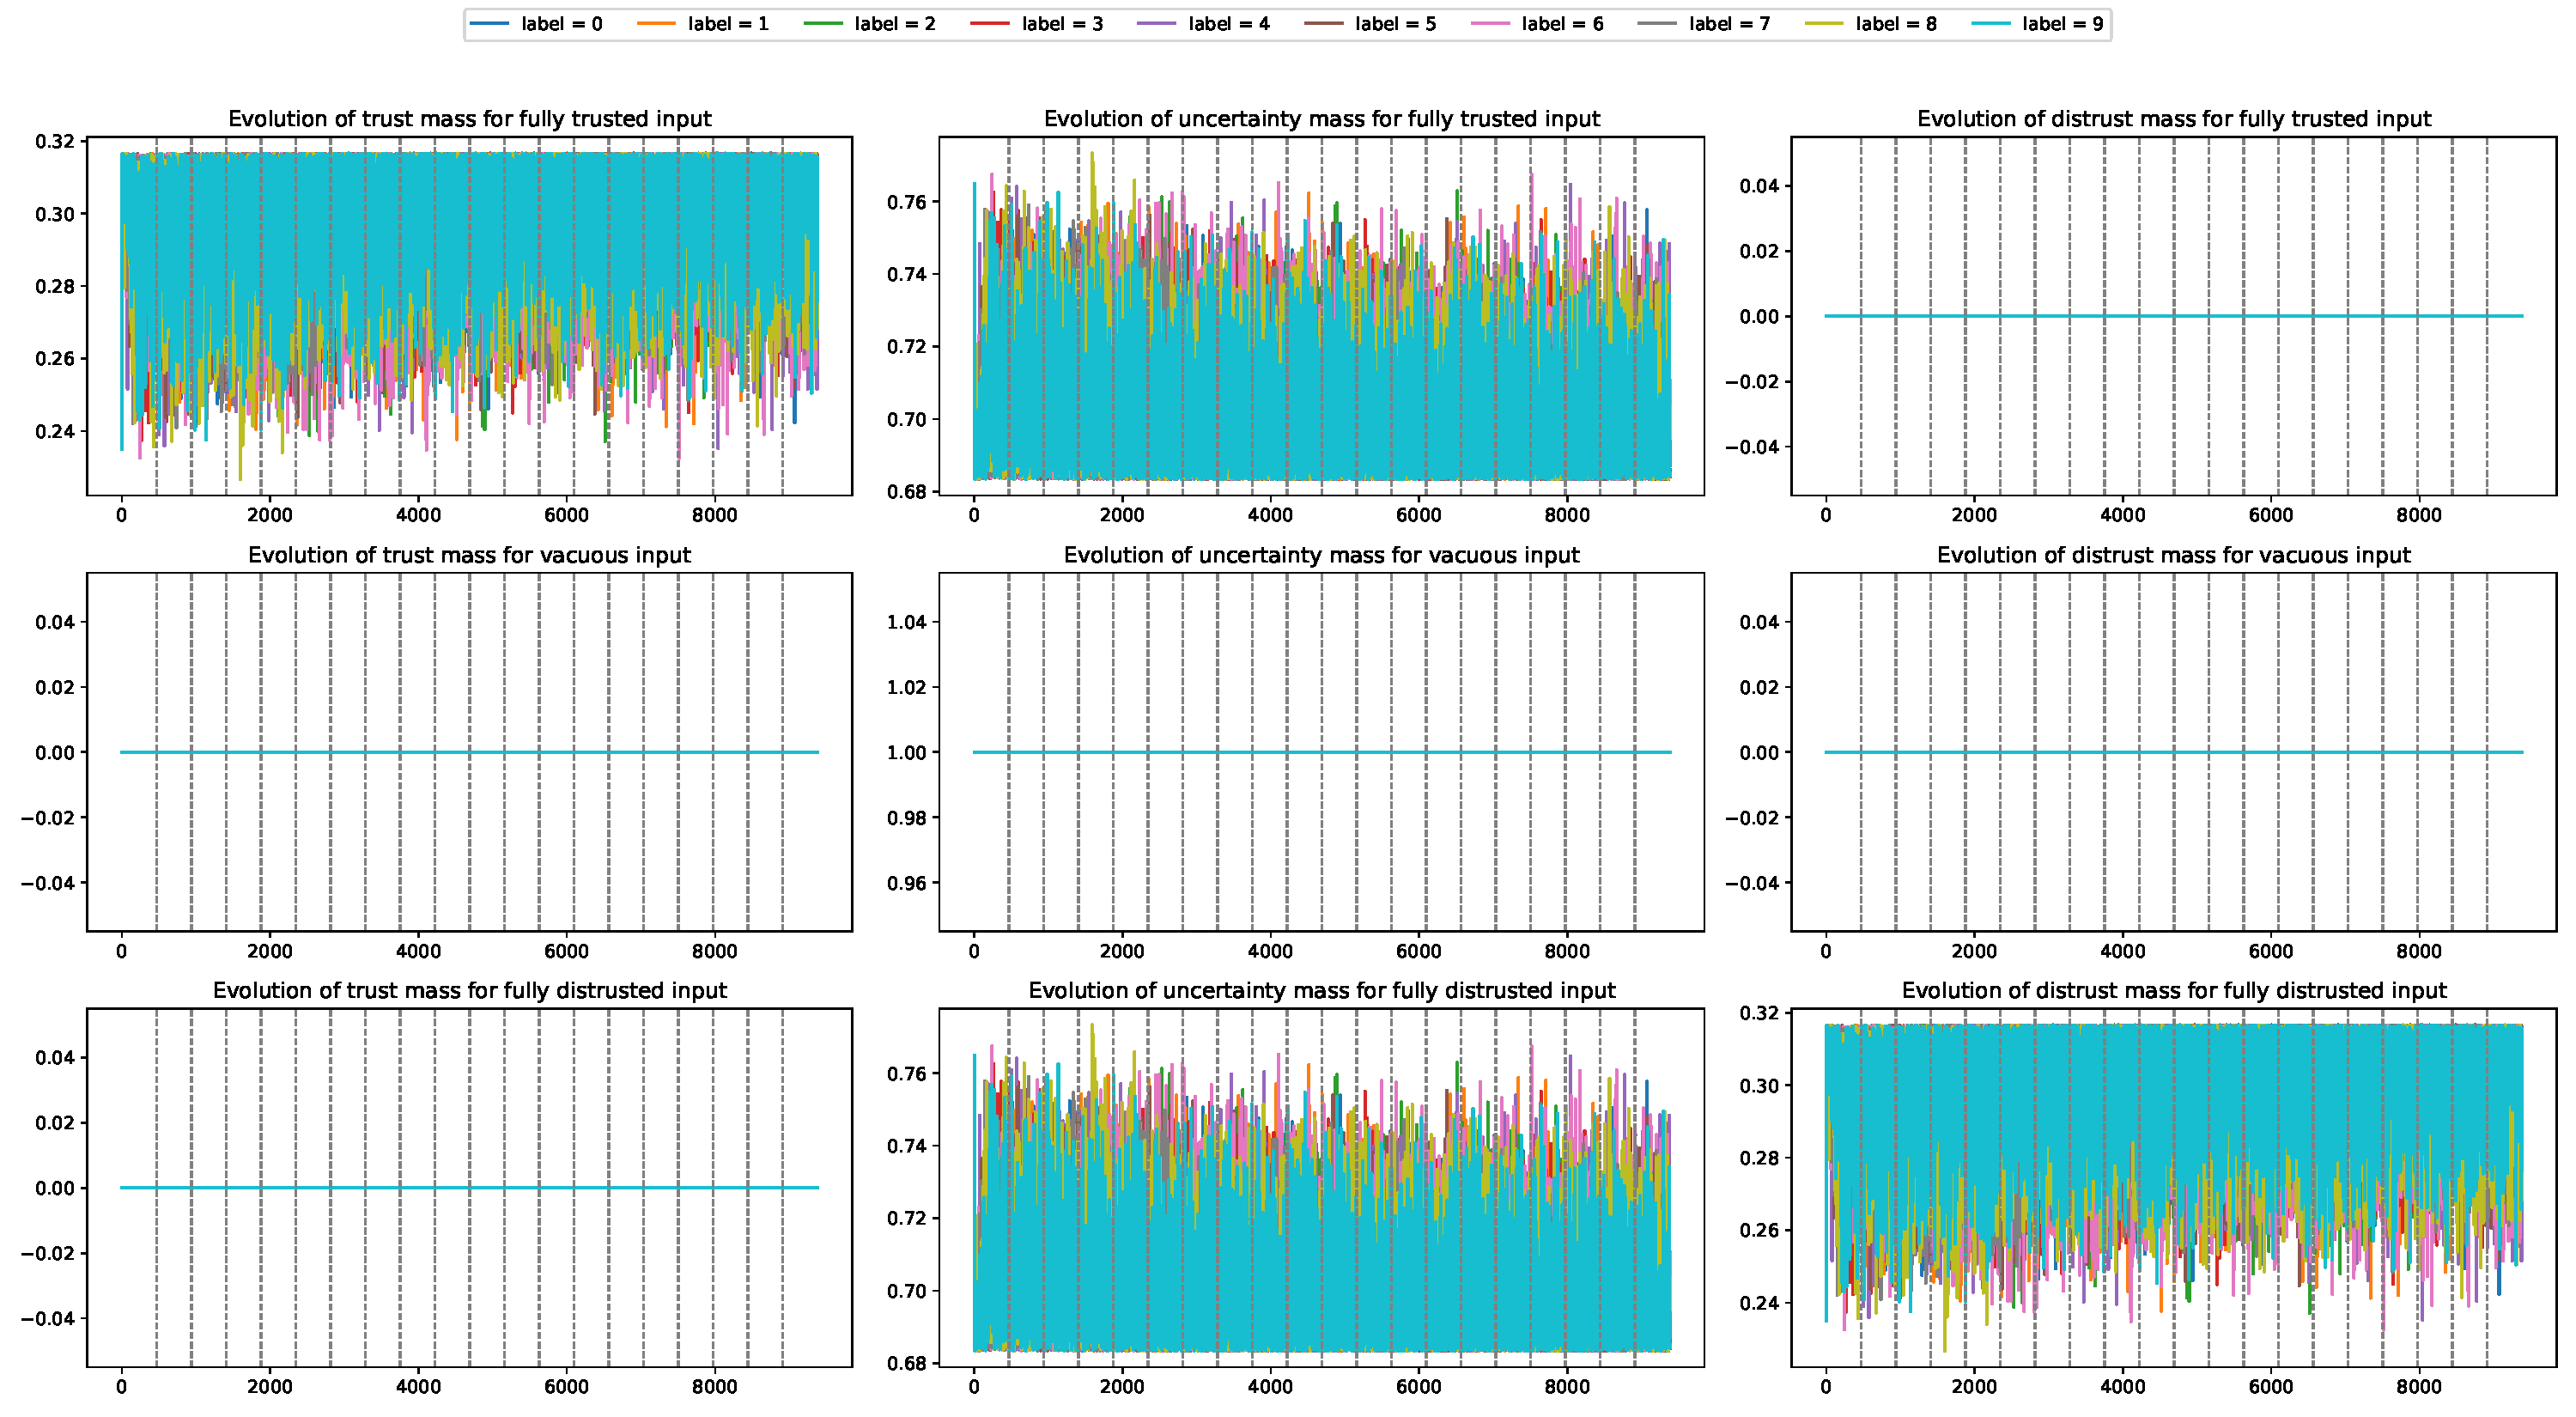
\includegraphics[width=\textwidth]{plots_v2/MNIST/architecture/plot_ptas-16-v-v.pdf}
  \caption{16 Hidden neurons}
\end{figure}
\begin{figure}[H]
  \centering
  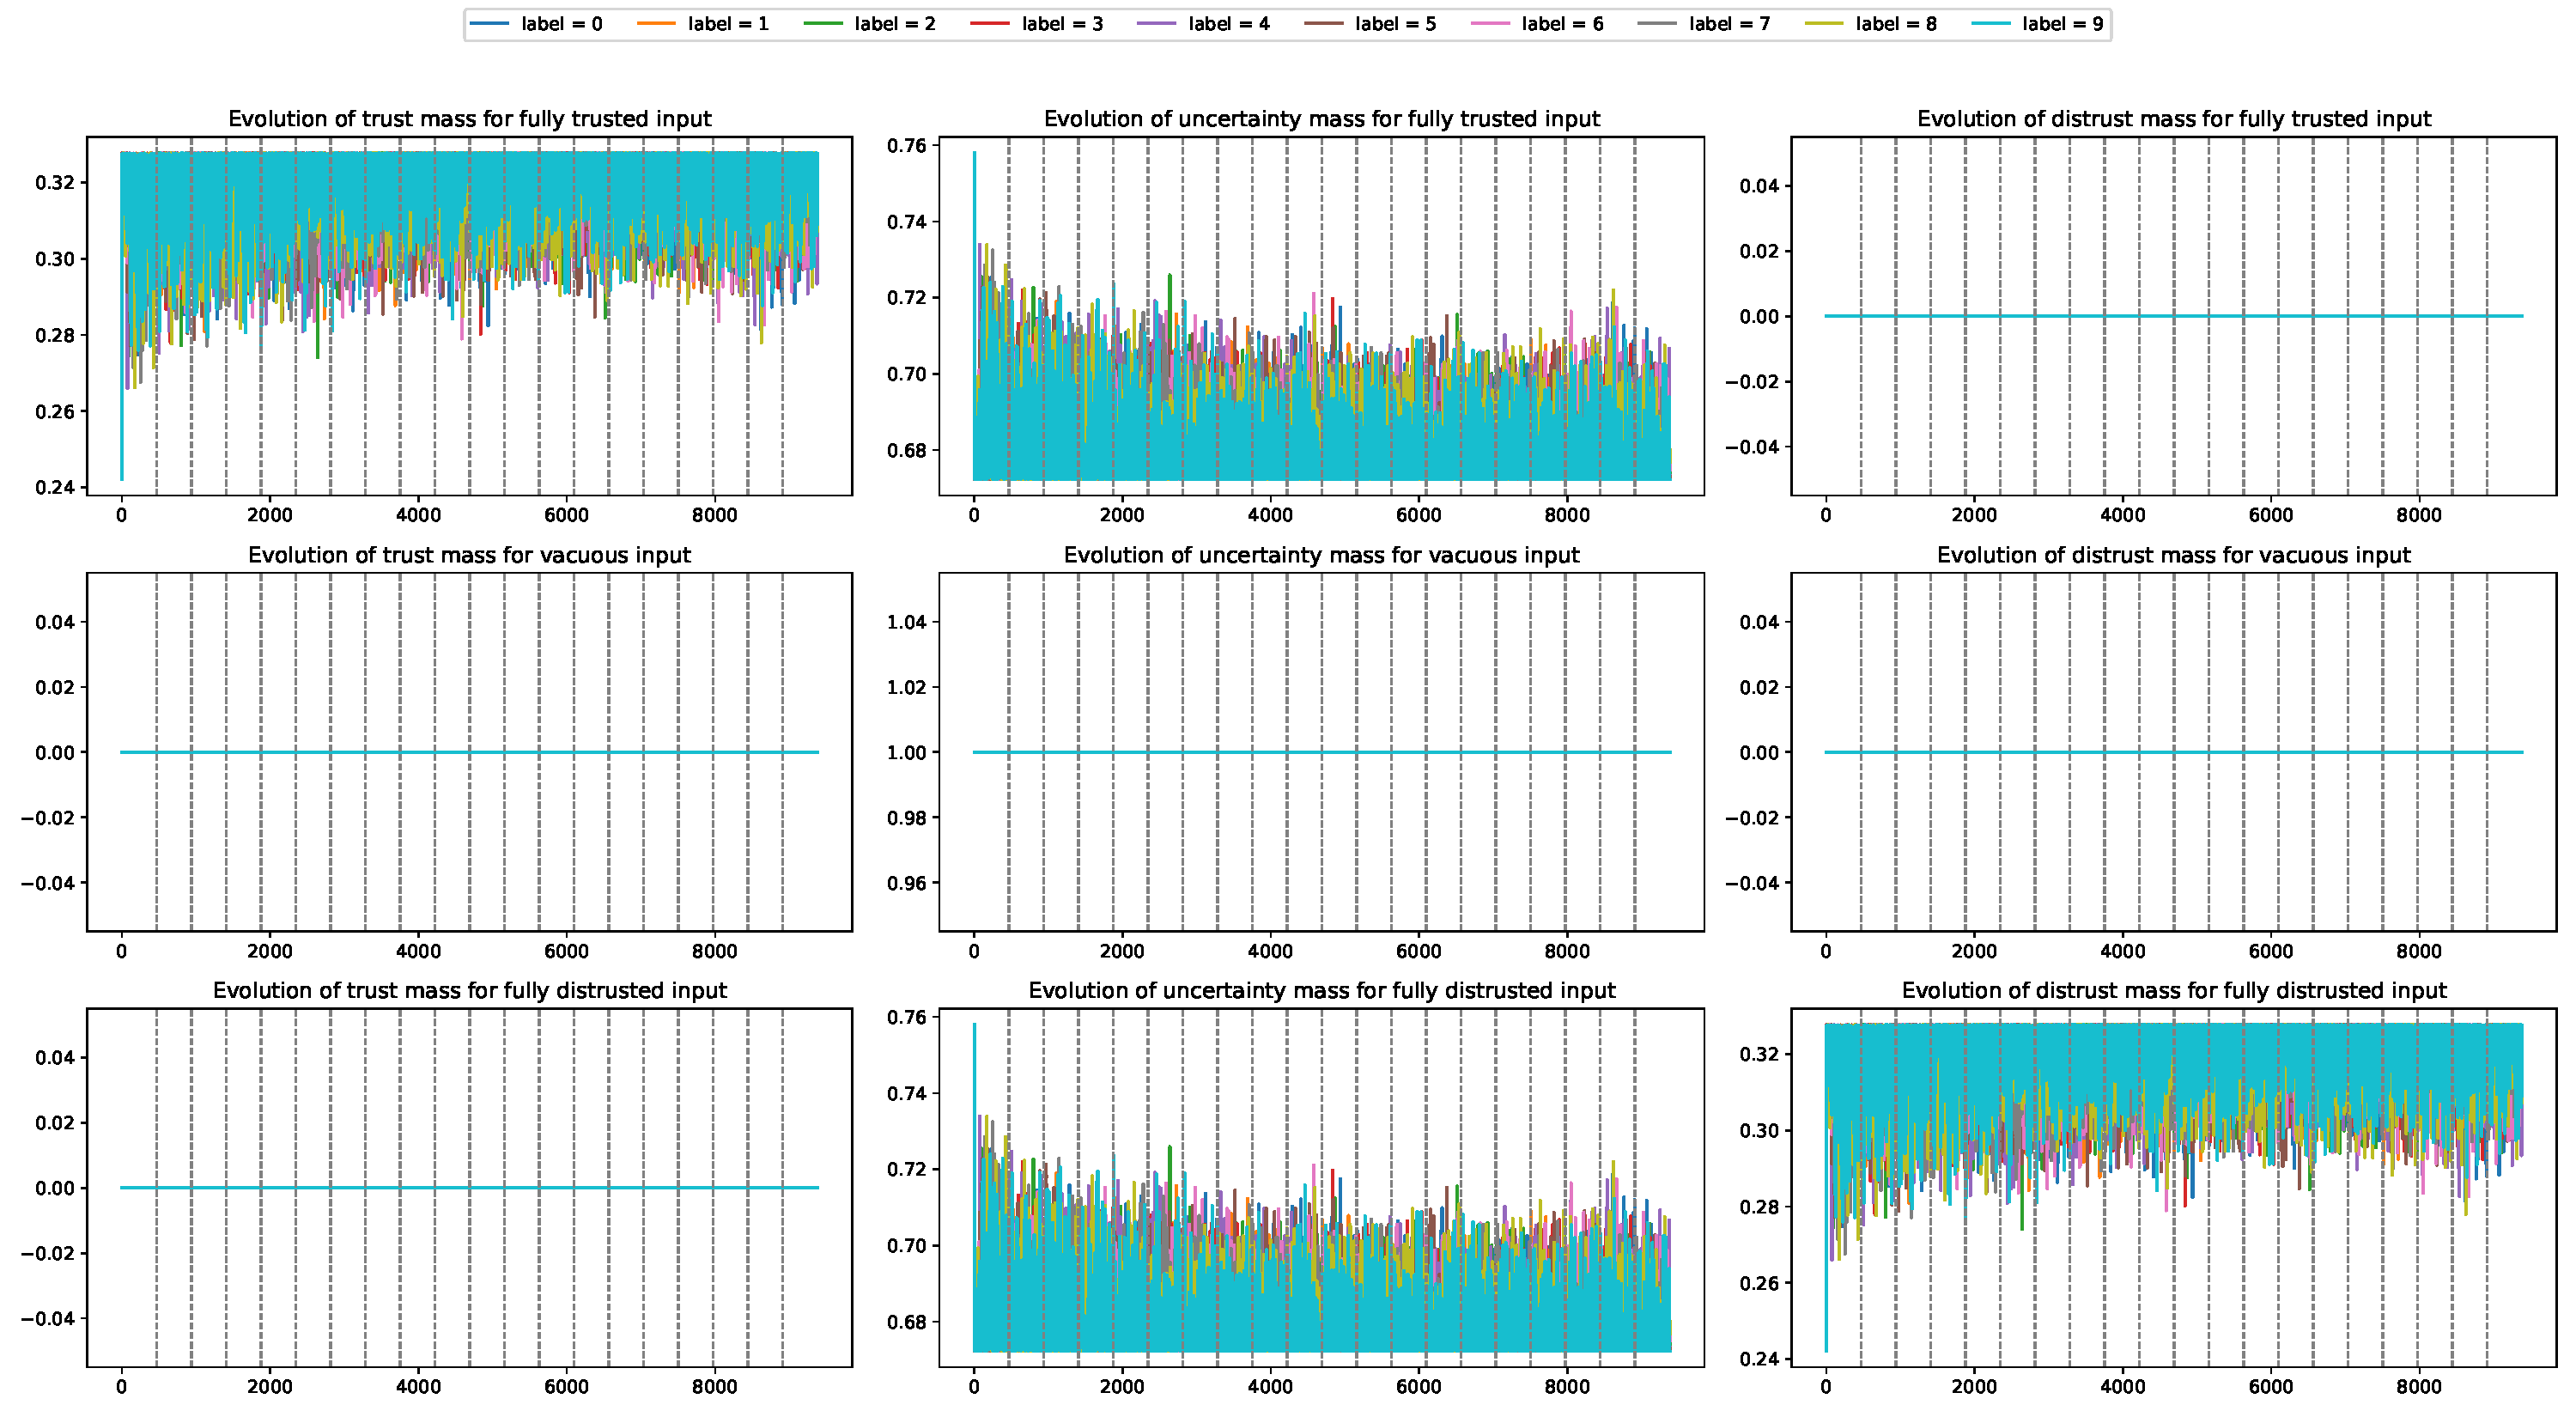
\includegraphics[width=\textwidth]{plots_v2/MNIST/architecture/plot_ptas-32-v-v.pdf}
  \caption{32 Hidden neurons}
\end{figure}
\begin{figure}[H]
  \centering
  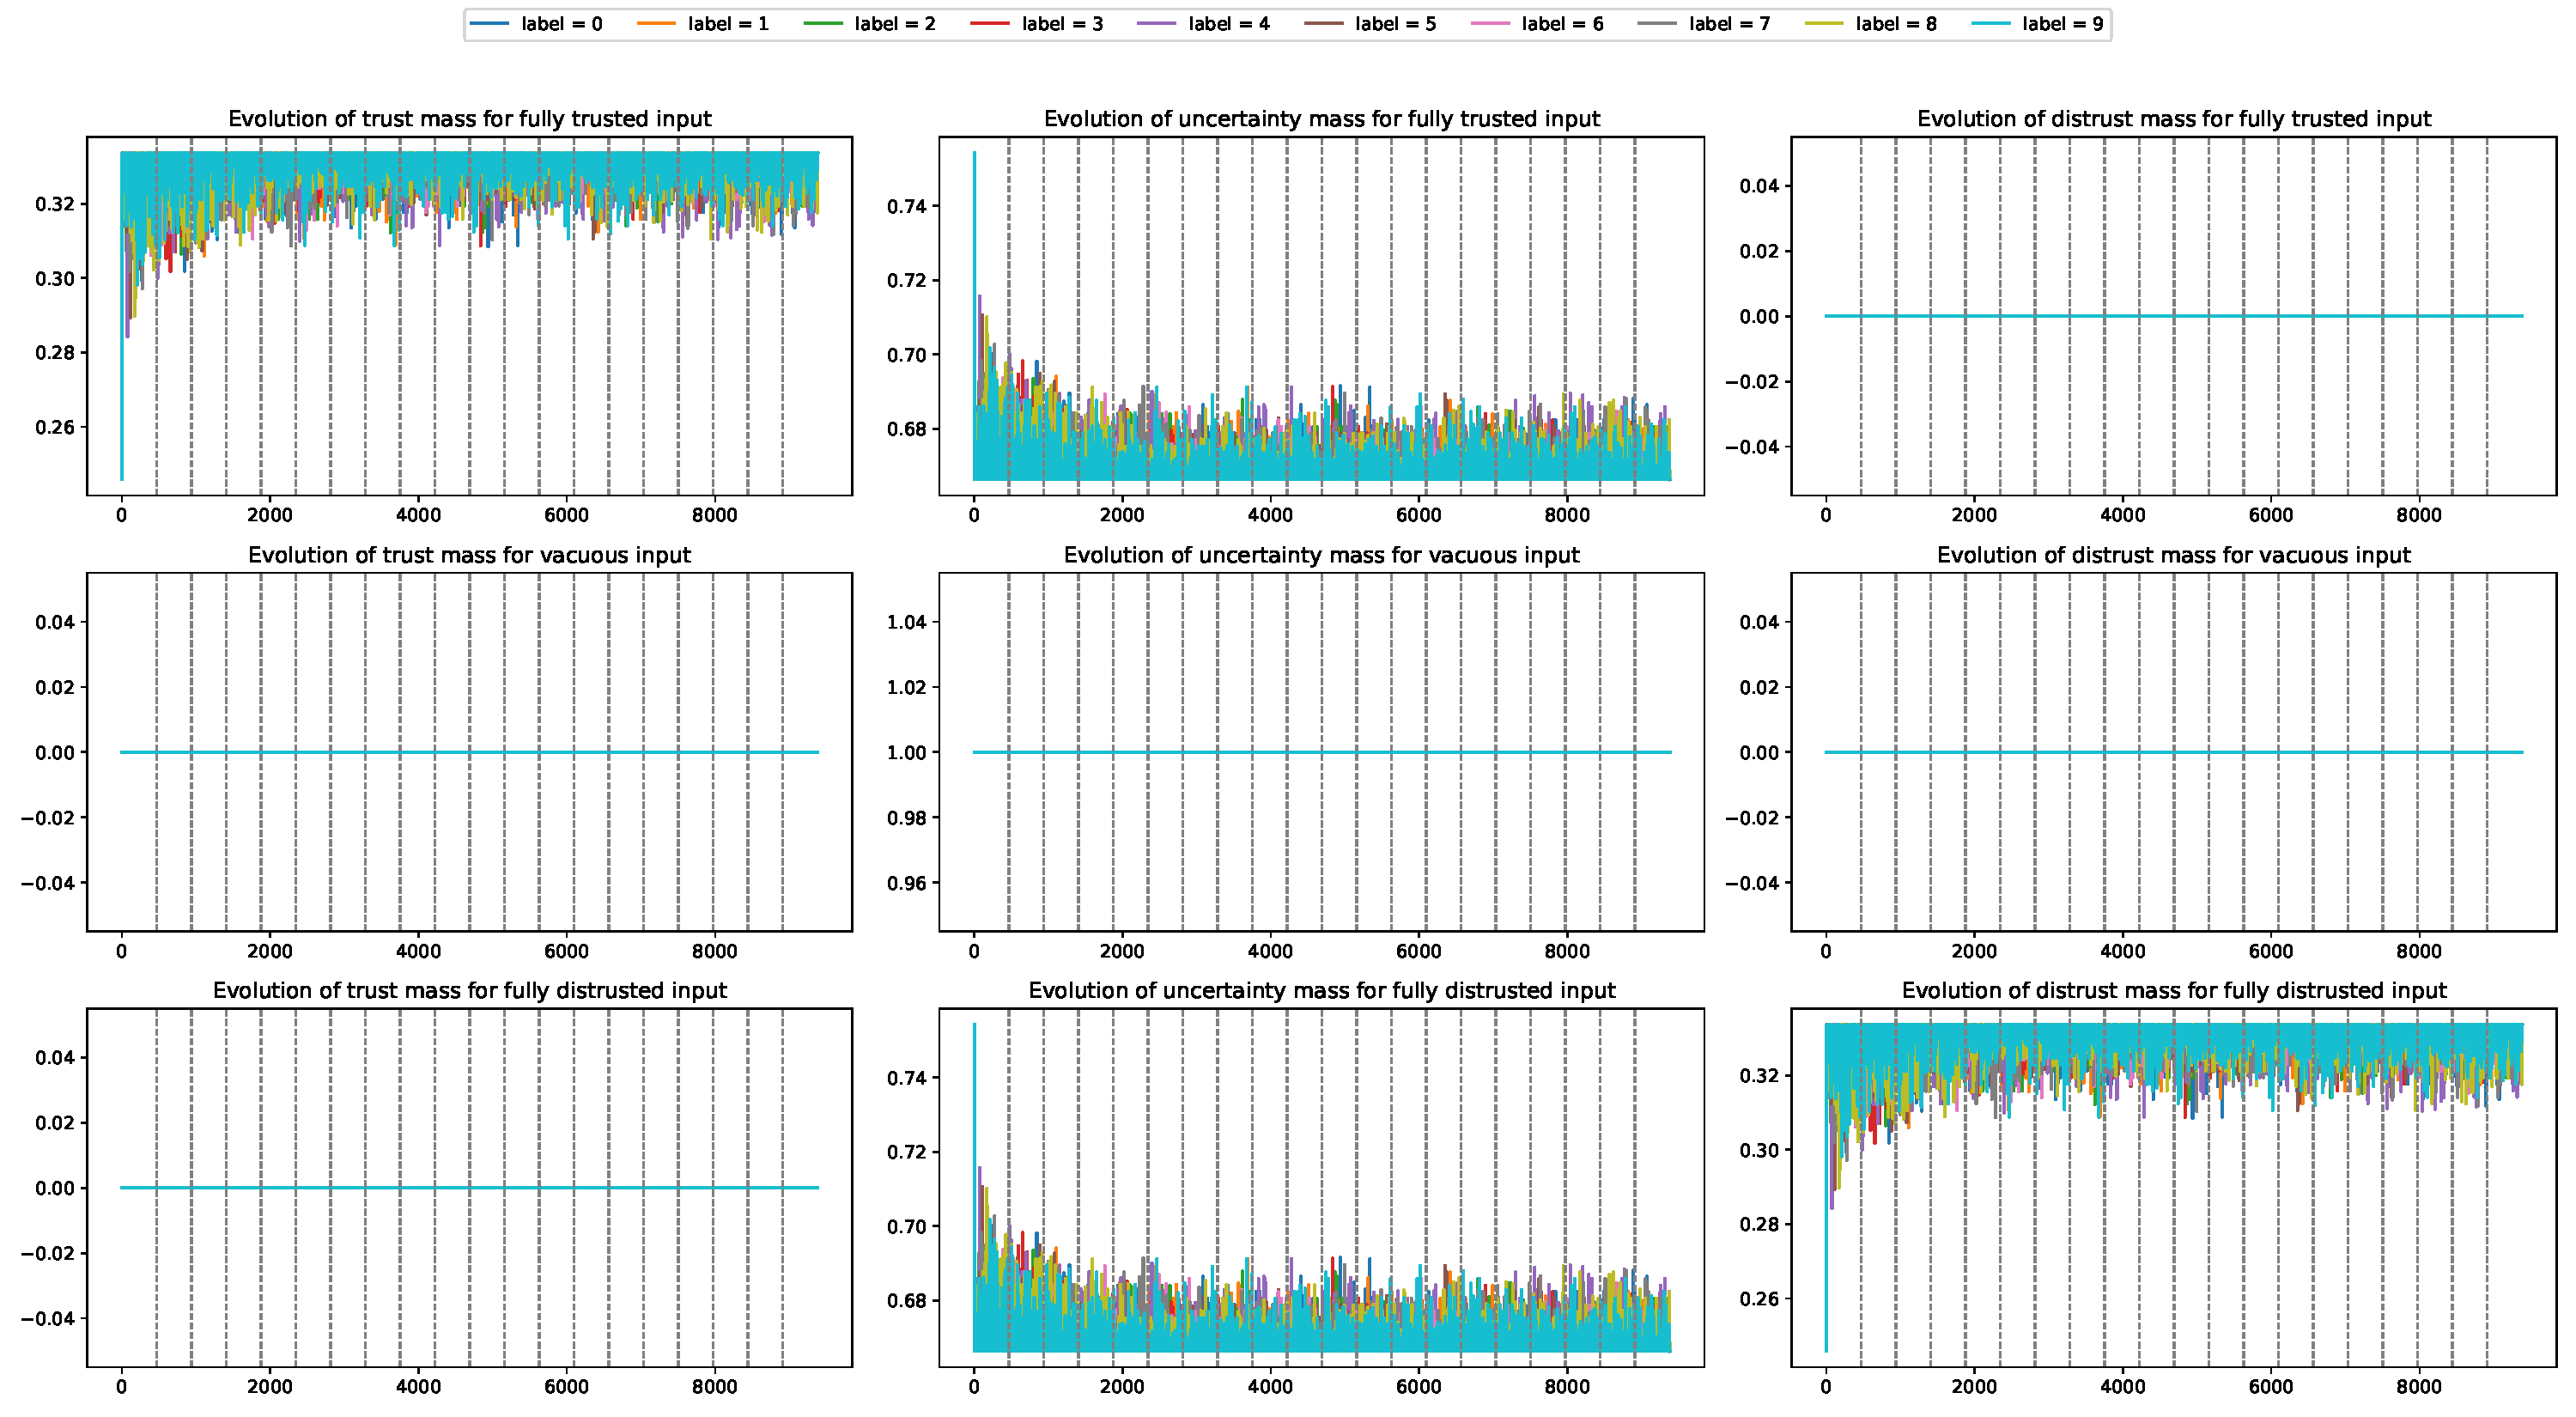
\includegraphics[width=\textwidth]{plots_v2/MNIST/architecture/plot_ptas-64-v-v.pdf}
  \caption{64 Hidden neurons}
\end{figure}
\begin{figure}[H]
  \centering
  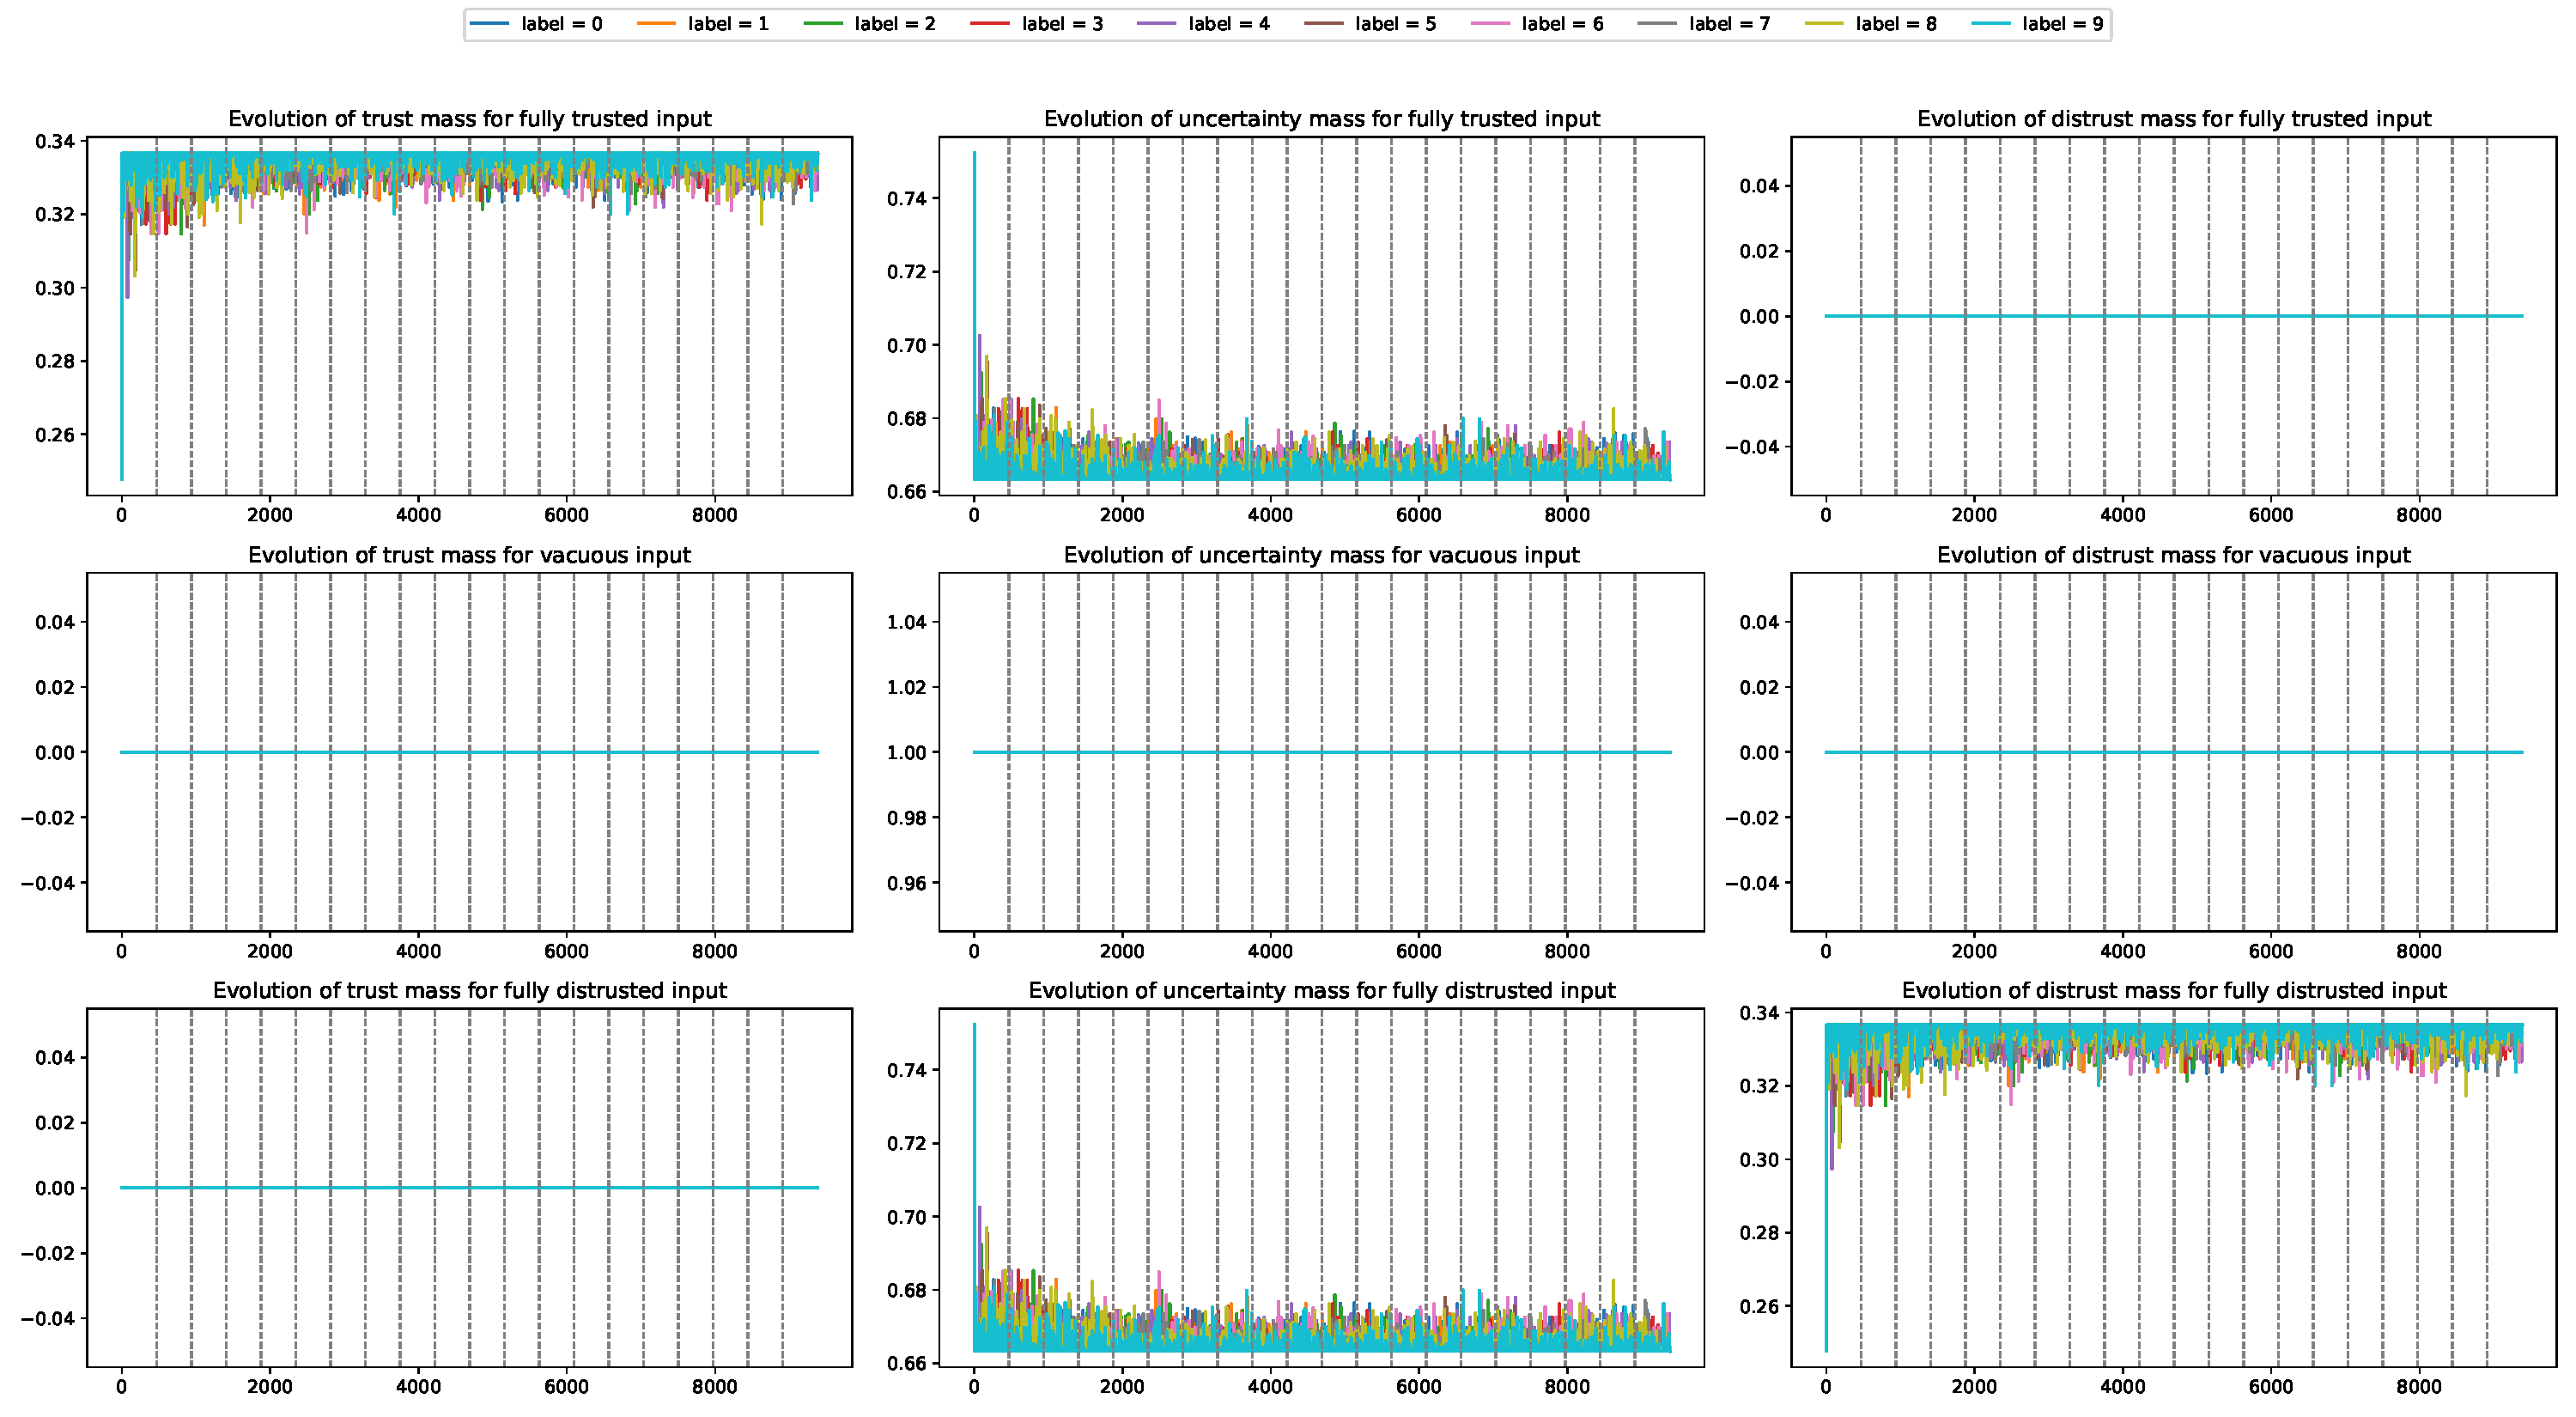
\includegraphics[width=\textwidth]{plots_v2/MNIST/architecture/plot_ptas-128-v-v.pdf}
  \caption{128 Hidden neurons}
\end{figure}
\begin{figure}[H]
  \centering
  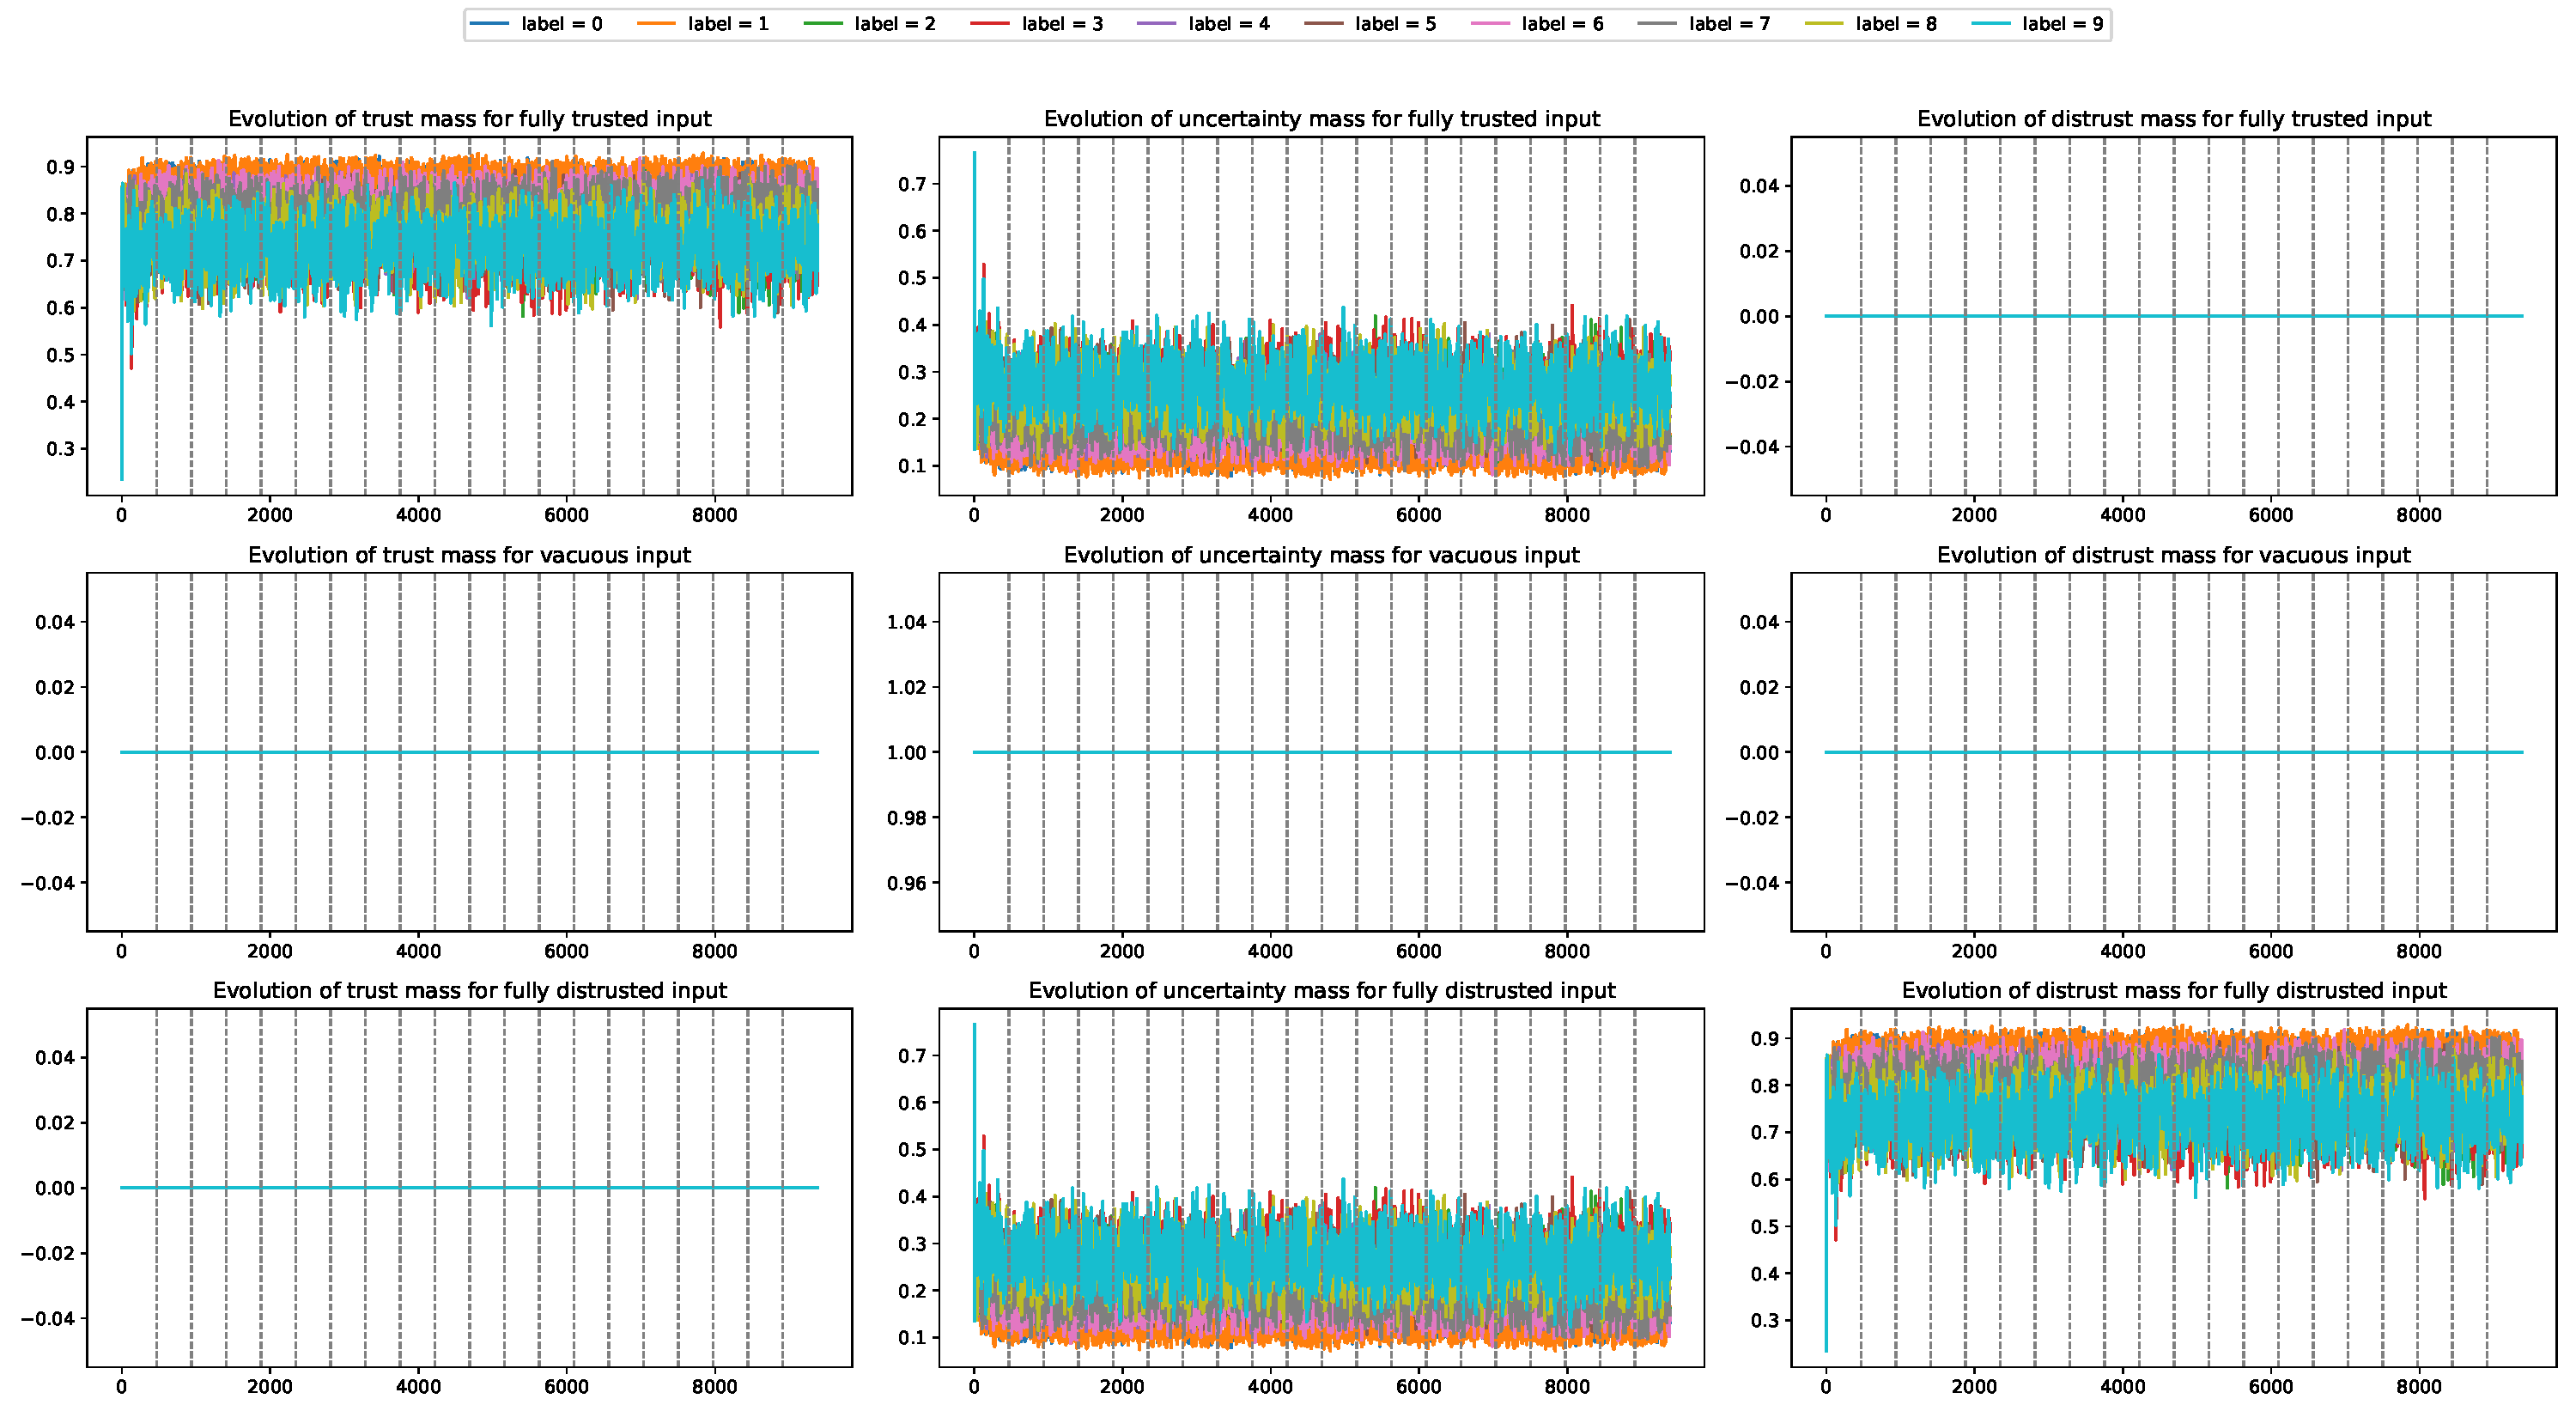
\includegraphics[width=\textwidth]{plots_v2/MNIST/architecture/plot_ptas-16-t-t.pdf}
  \caption{16 Hidden neurons with Fully Trusted Assessment}
\end{figure}

\subsection{MNIST poisoned 128 hidden neurons (\cref{exp:3})}\label{sec:resmnistpois}
\begin{figure}[H]
  \centering
  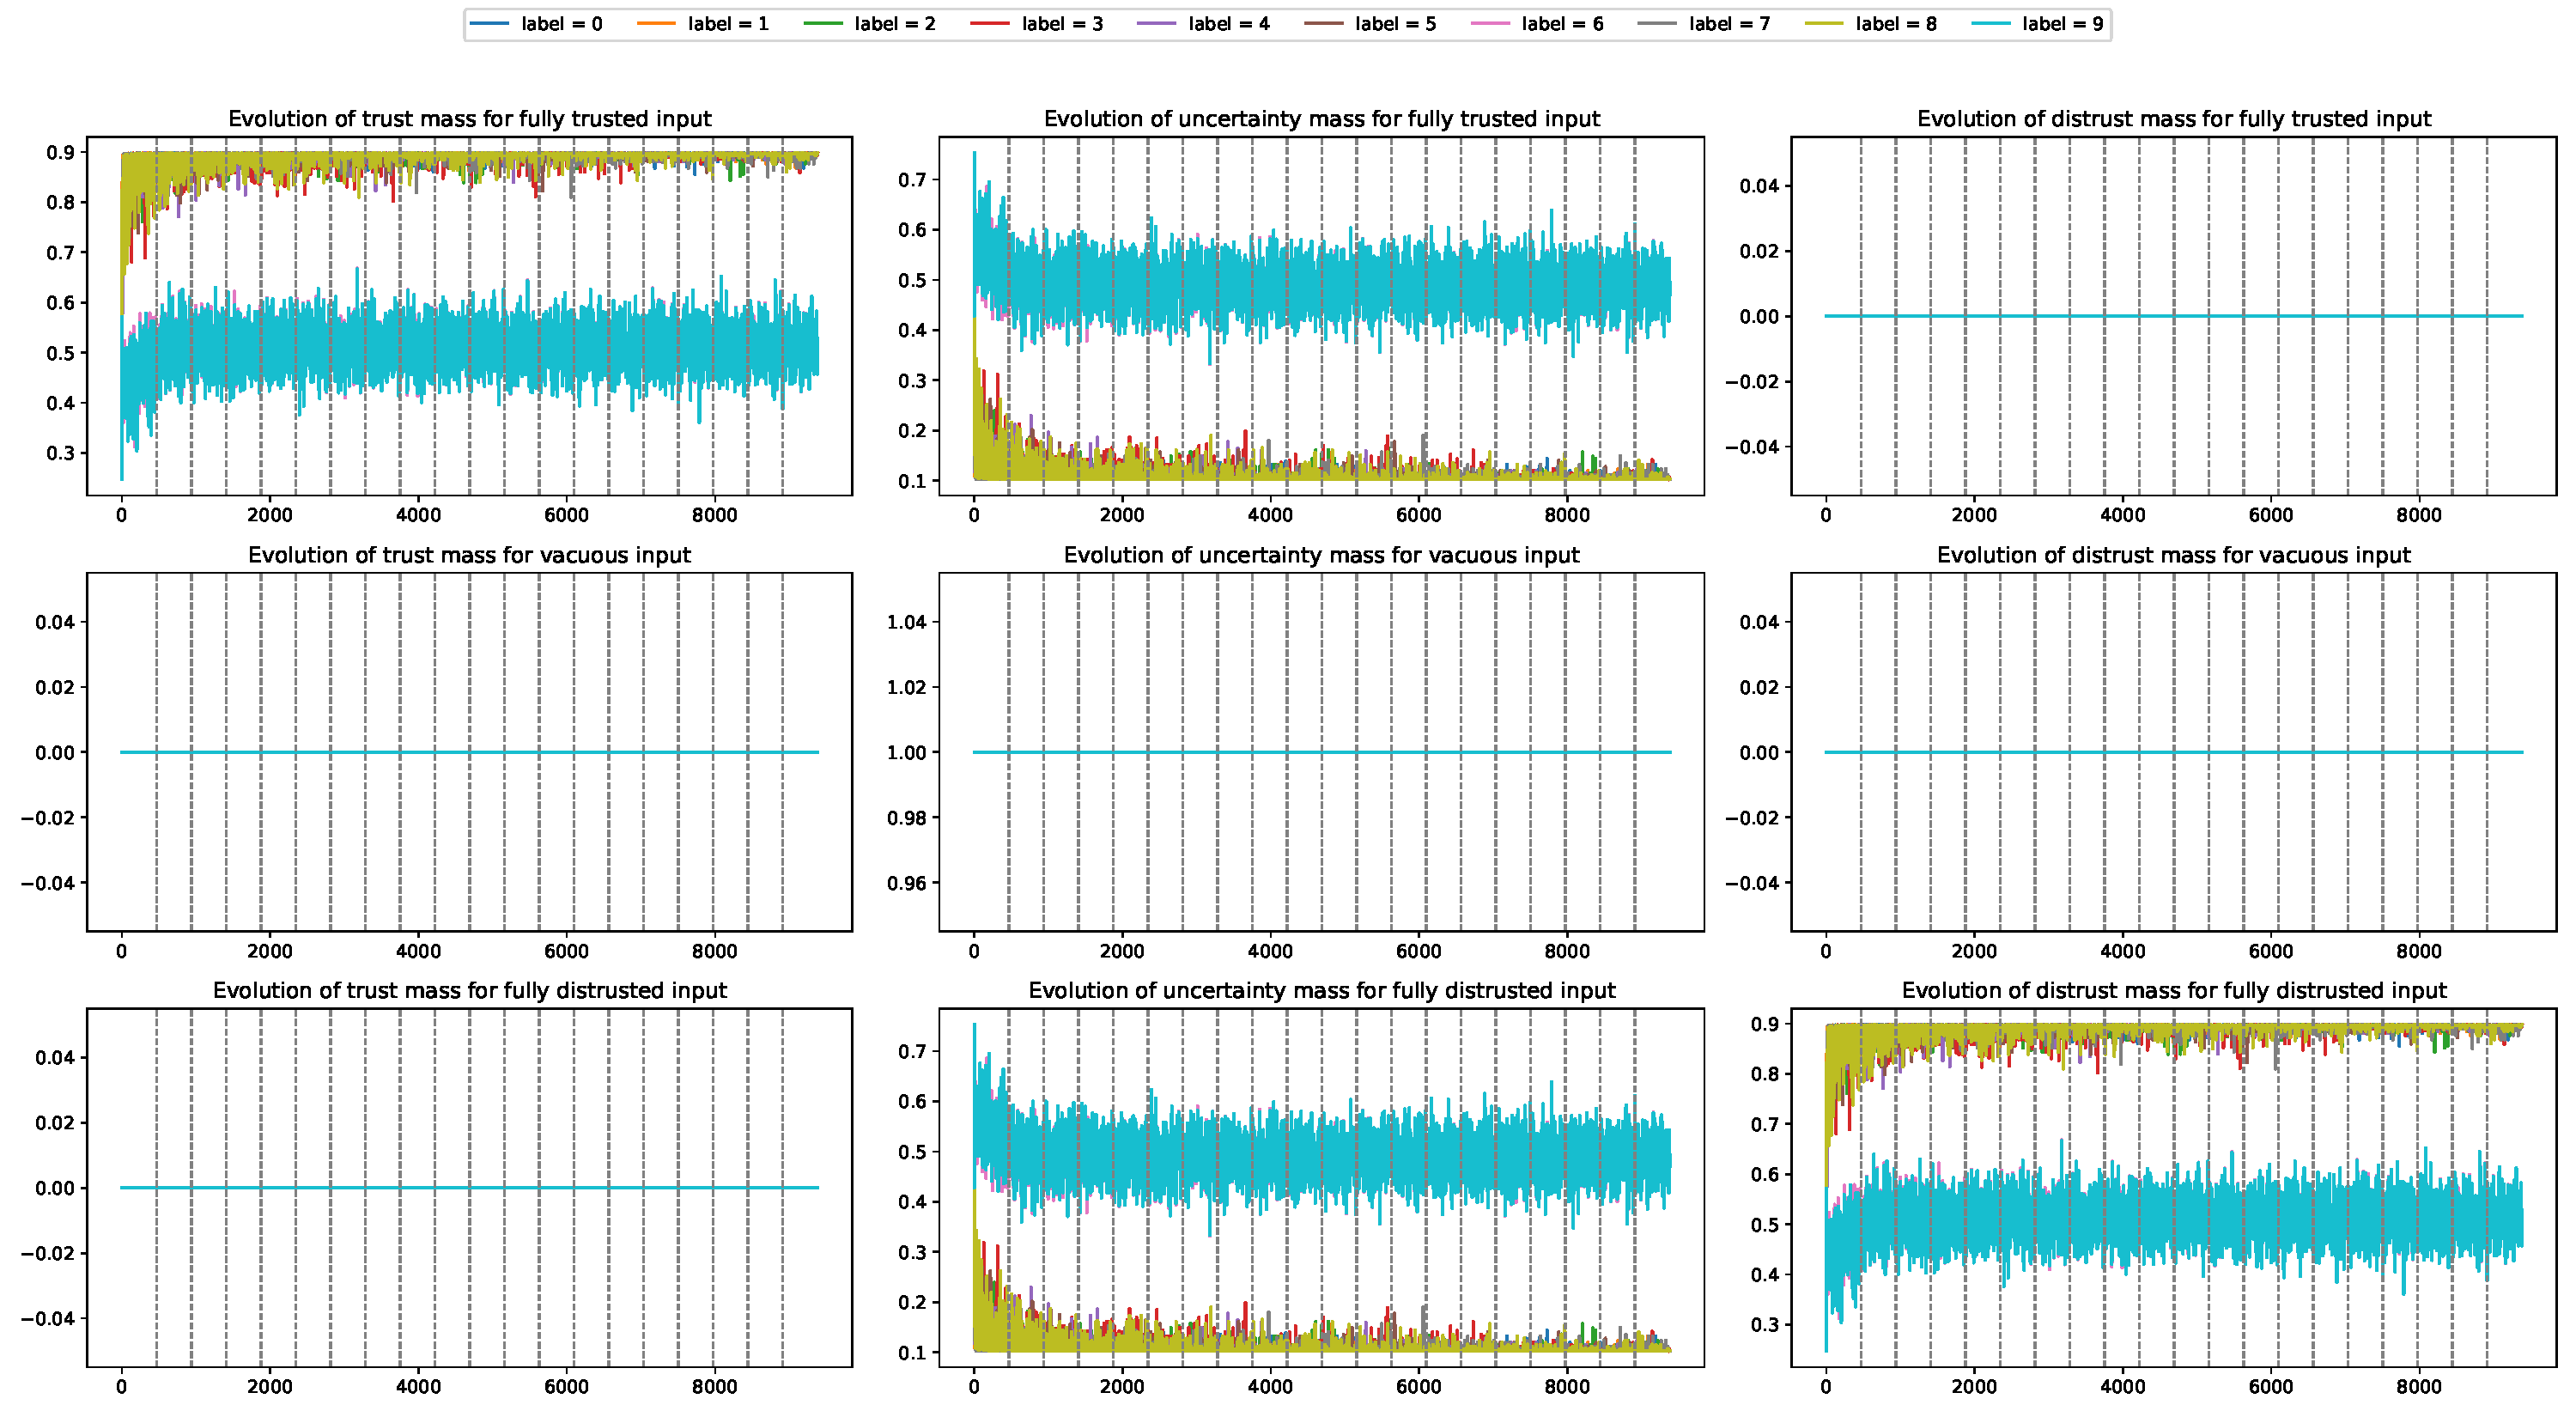
\includegraphics[width=\textwidth]{plots_v2/MNIST/poisoned/plot_ptas-128-t-t-ps1.pdf}
  \caption{1 pixel}
\end{figure}
\begin{figure}[H]
  \centering
  \includegraphics[width=\textwidth]{plots_v2/MNIST/poisoned/plot_ptas-128-t-t-ps4.pdf}
  \caption{4×4 pixels}
\end{figure}
\begin{figure}[H]
  \centering
  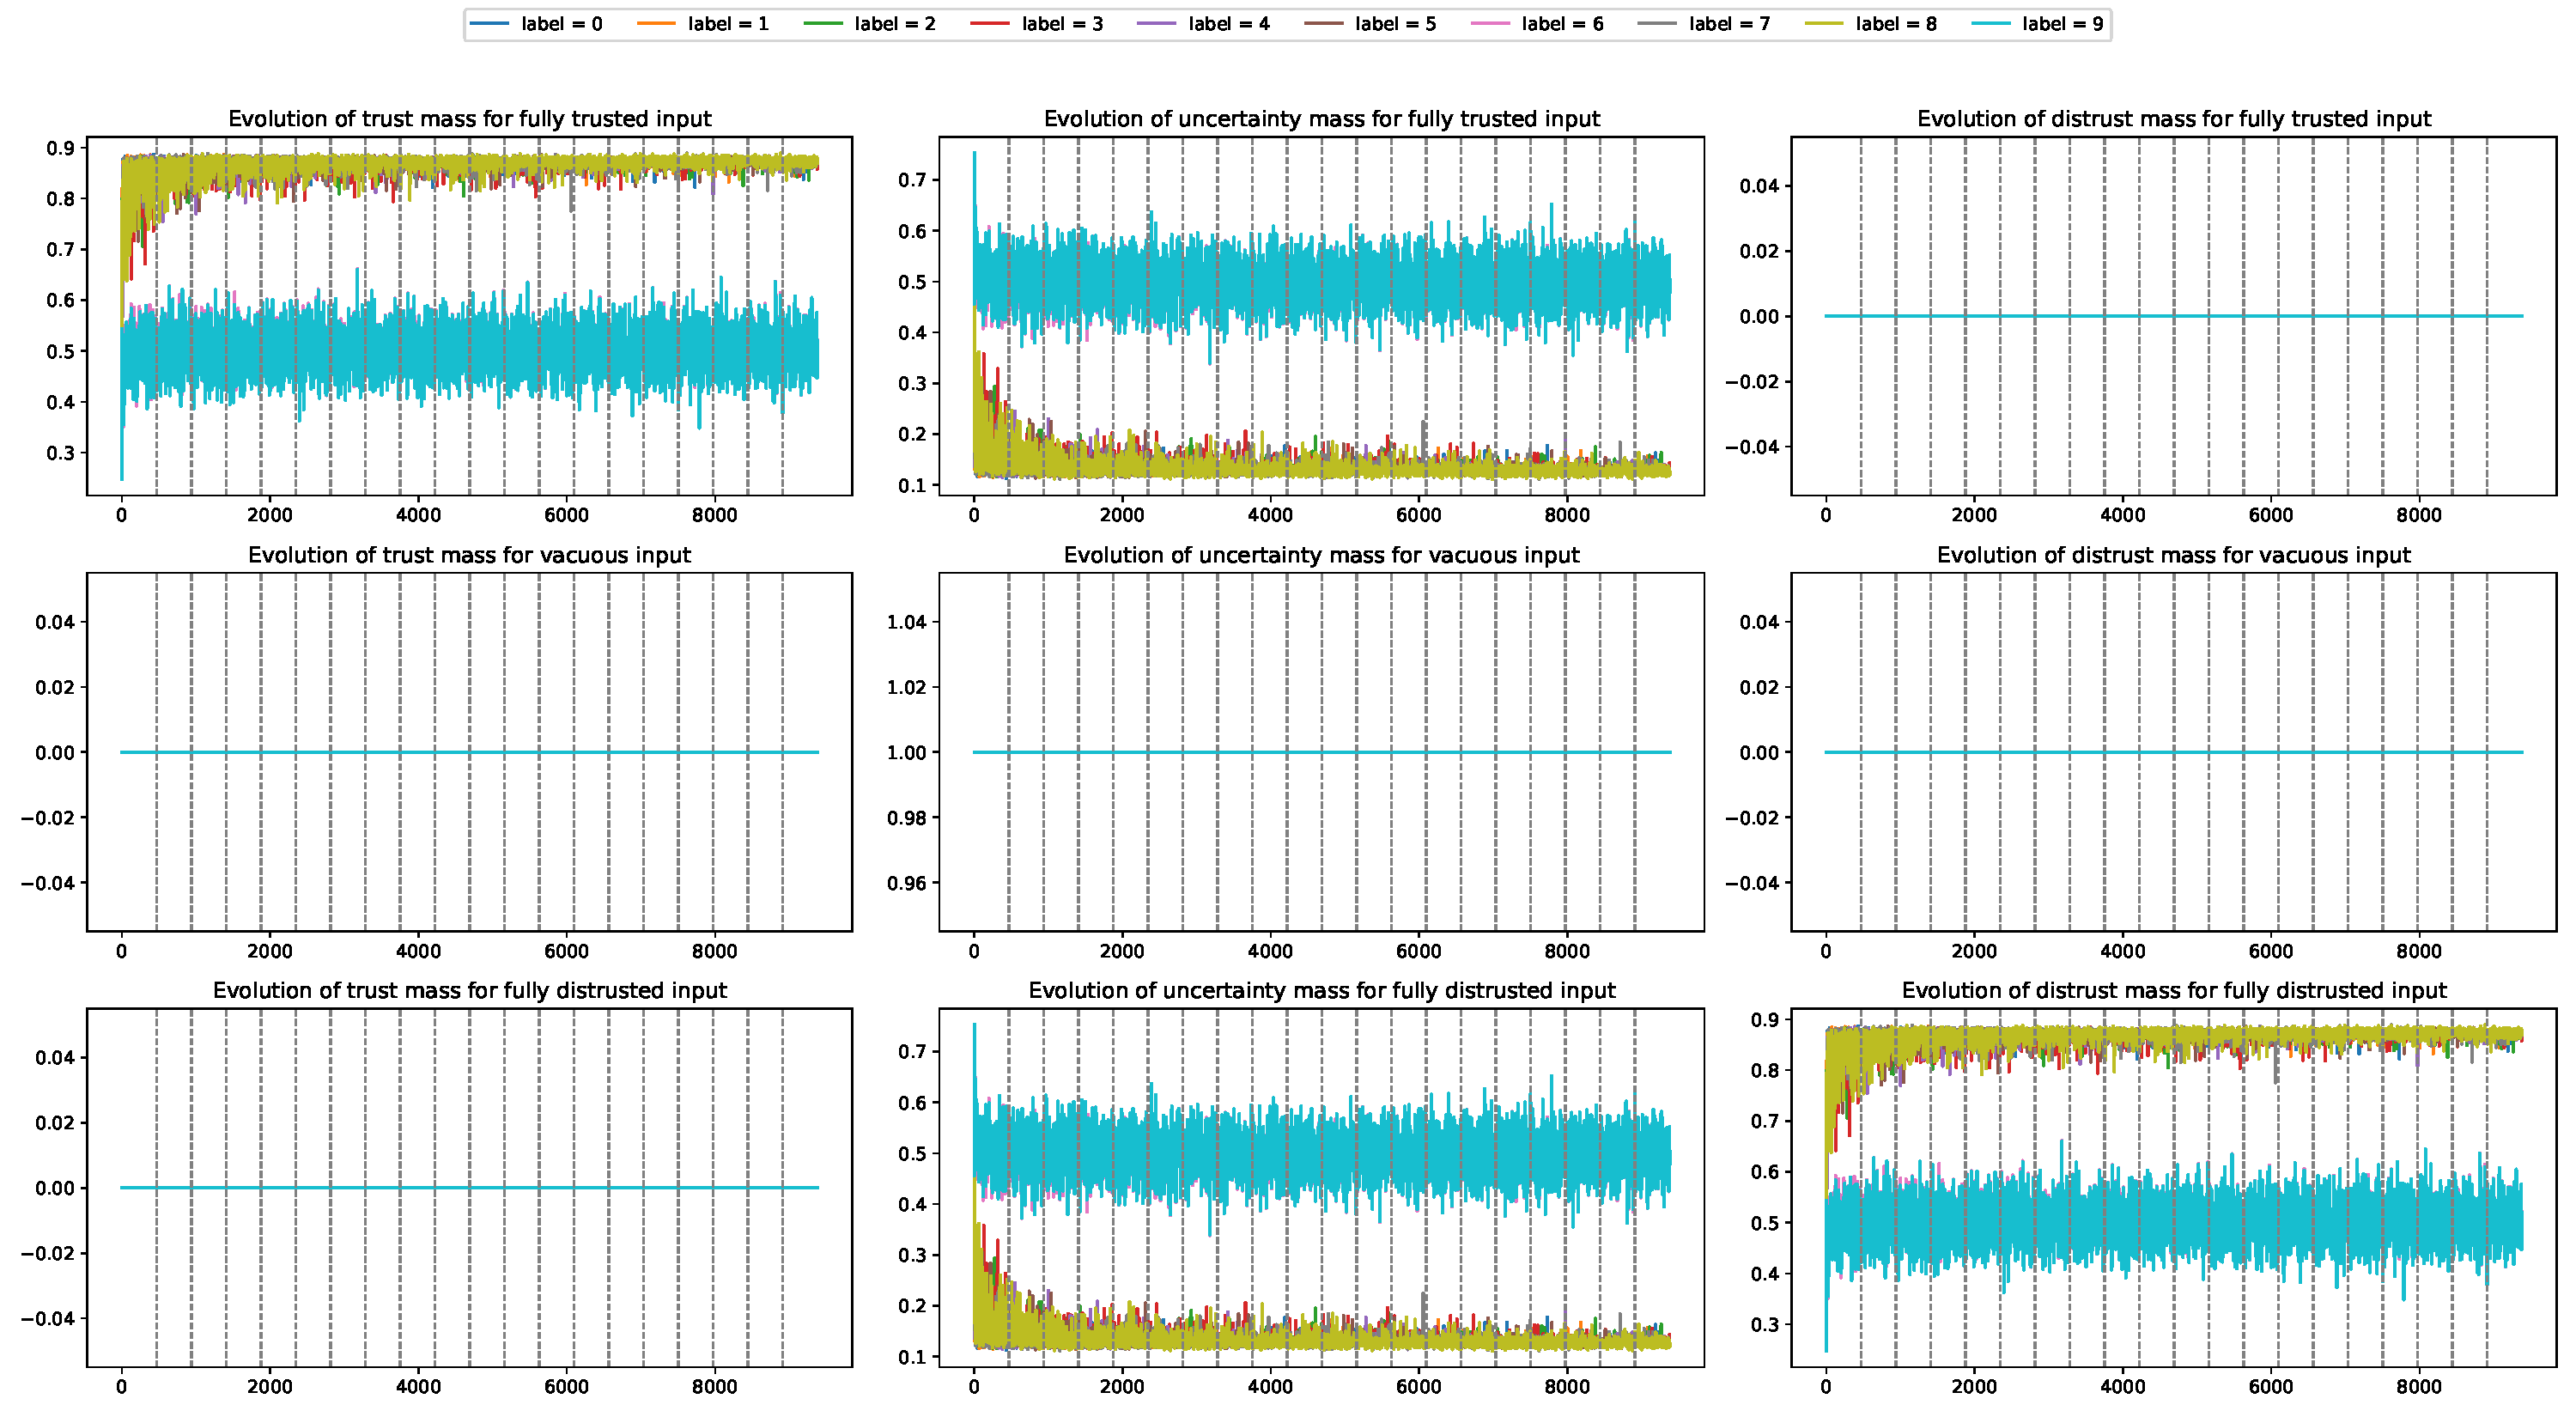
\includegraphics[width=\textwidth]{plots_v2/MNIST/poisoned/plot_ptas-128-t-t-ps10.pdf}
  \caption{10×10 pixels}
\end{figure}
\begin{figure}[H]
  \centering
  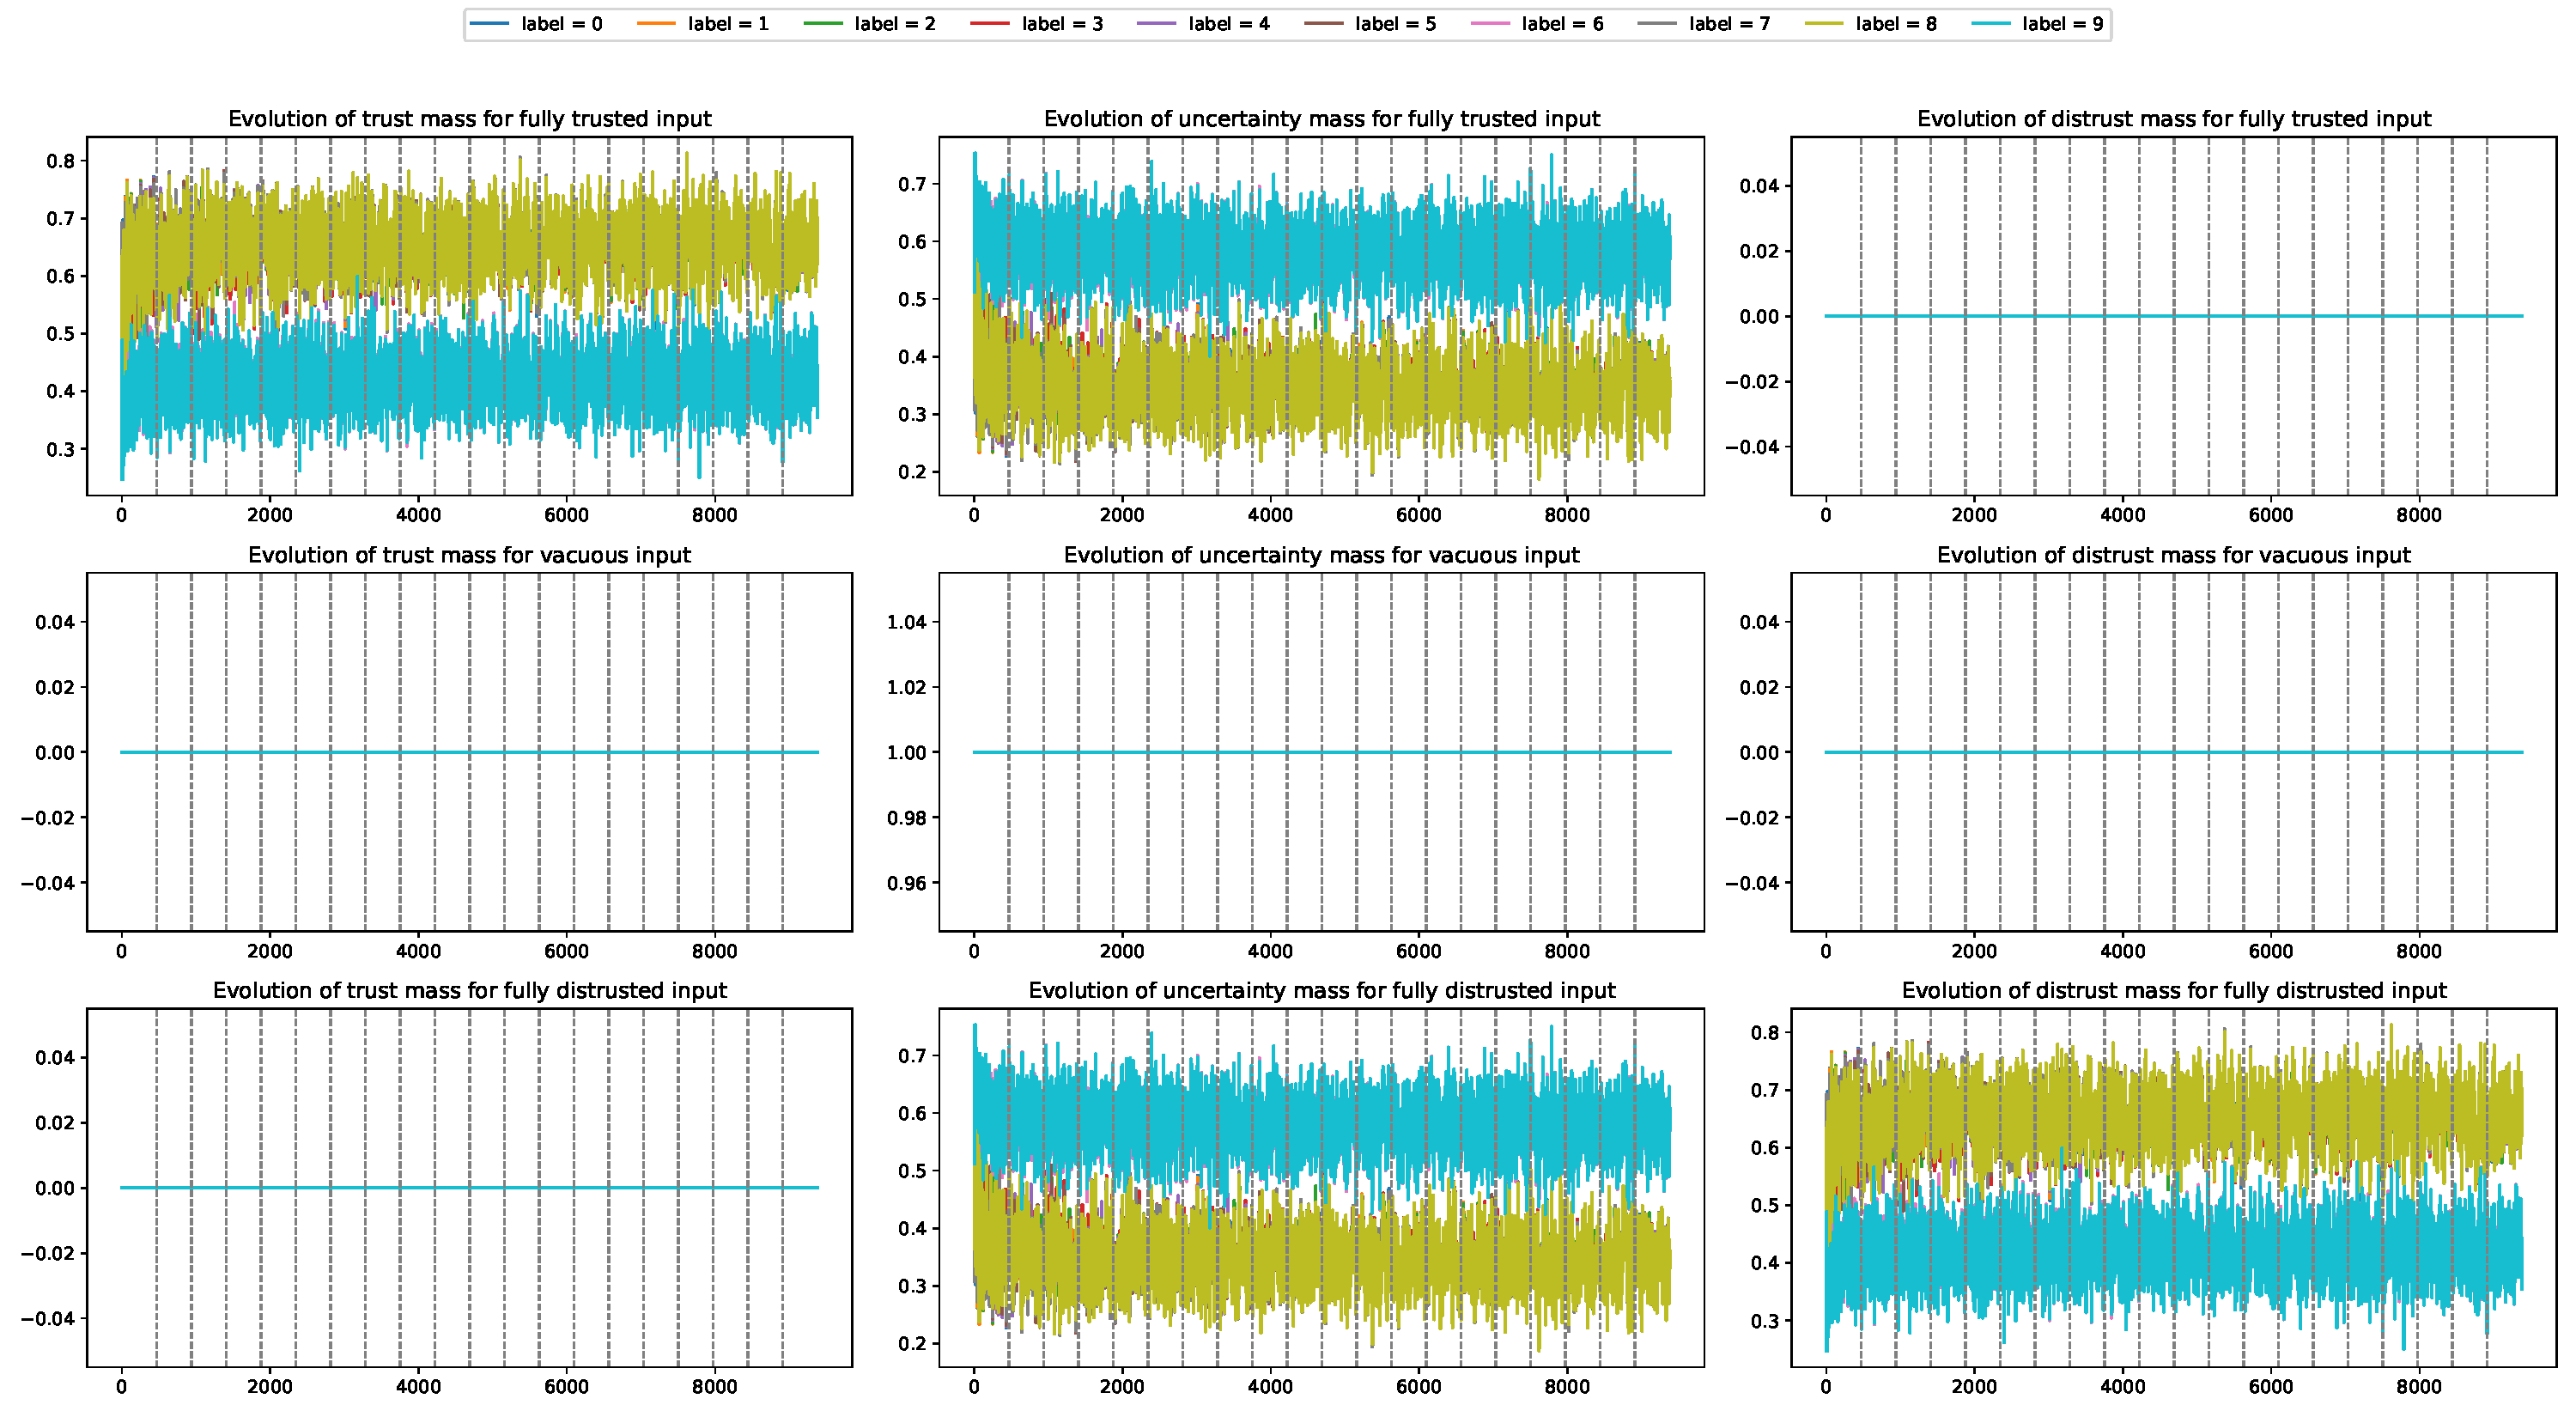
\includegraphics[width=\textwidth]{plots_v2/MNIST/poisoned/plot_ptas-128-t-t-ps27.pdf}
  \caption{27×27 pixels}
\end{figure}
\subsection{Plots for the Comparative Trust Evaluation (\cref{exp:4})}\label{sec:resexp4}
\begin{figure}[H]
  \centering
  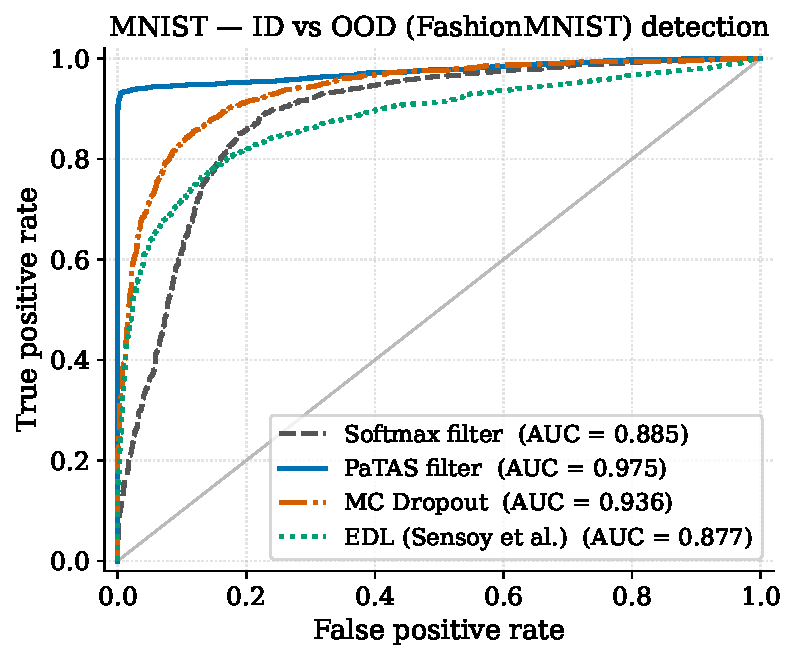
\includegraphics[width=0.62\textwidth]{plots_v2/exp4/roc_ood_mnist.pdf}
  \caption{Out-of-distribution detection ROC (MNIST in-distribution vs.\ Fashion-MNIST OOD): each method's own score as the discriminator. Curves and legend AUC values are from a single representative evaluation seed; \cref{tab:comparative} reports mean $\pm$ std over three seeds.}
\end{figure}
\begin{figure}[H]
  \centering
  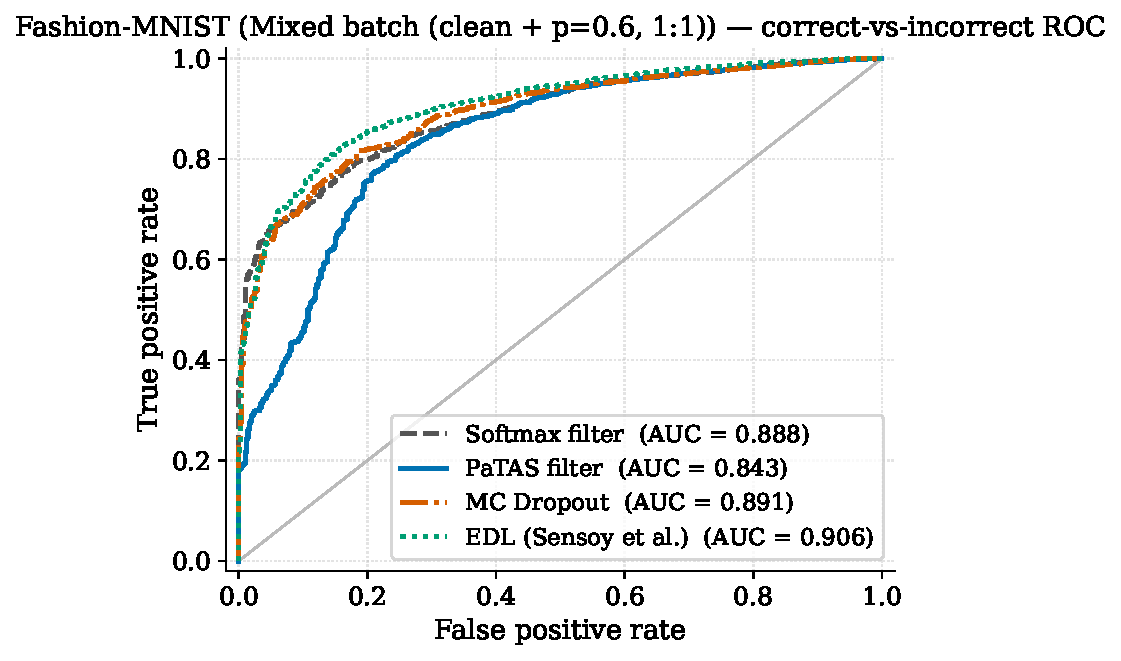
\includegraphics[width=0.62\textwidth]{plots_v2/exp4/roc_mixed_fashion.pdf}
  \caption{Correct-vs-incorrect ROC on the Fashion-MNIST mixed batch (clean + corrupted inputs pooled 1:1), single representative evaluation seed.}
\end{figure}
\begin{figure}[H]
  \centering
  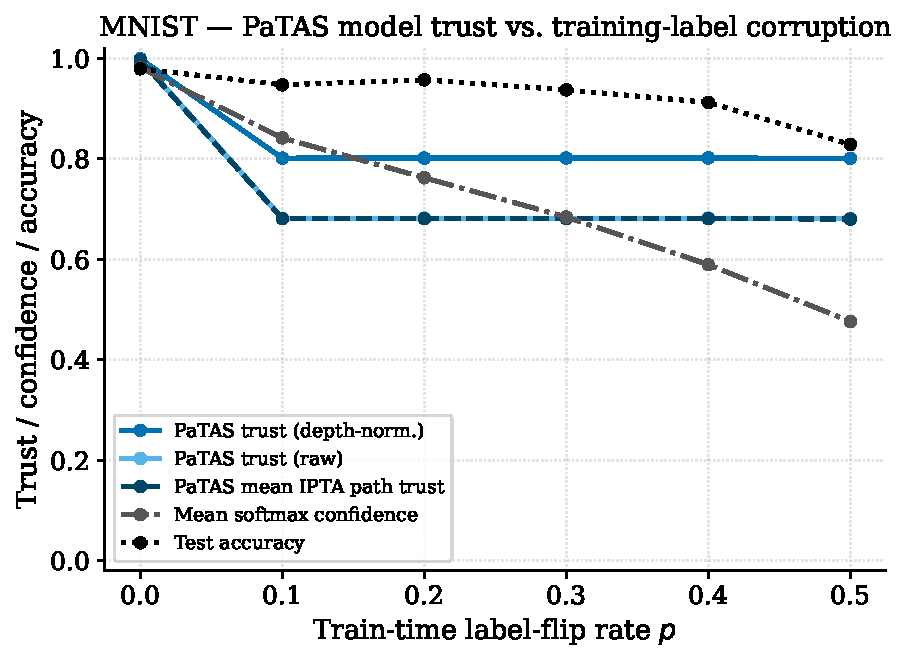
\includegraphics[width=0.62\textwidth]{plots_v2/exp4/model_trust_vs_labelnoise.pdf}
  \caption{Training-quality audit (\cref{tab:audit}): PaTAS model-side trust, mean softmax confidence, and test accuracy as functions of the train-time label-flip rate $p$. The depth-normalized curve rescales the committed mass $b+d$ of the aggregated opinion to $(b+d)^{1/L}$, with $L$ the number of trust-propagation layers, making trust comparable across network depths. Trust drops as a tripwire at any non-zero rate without using test data; confidence tracks severity but requires a clean labelled test set.}
\end{figure}

\subsection{Example for random dataset trust assessment}\label{sec:resrand}

\begin{figure}[H]
\centering
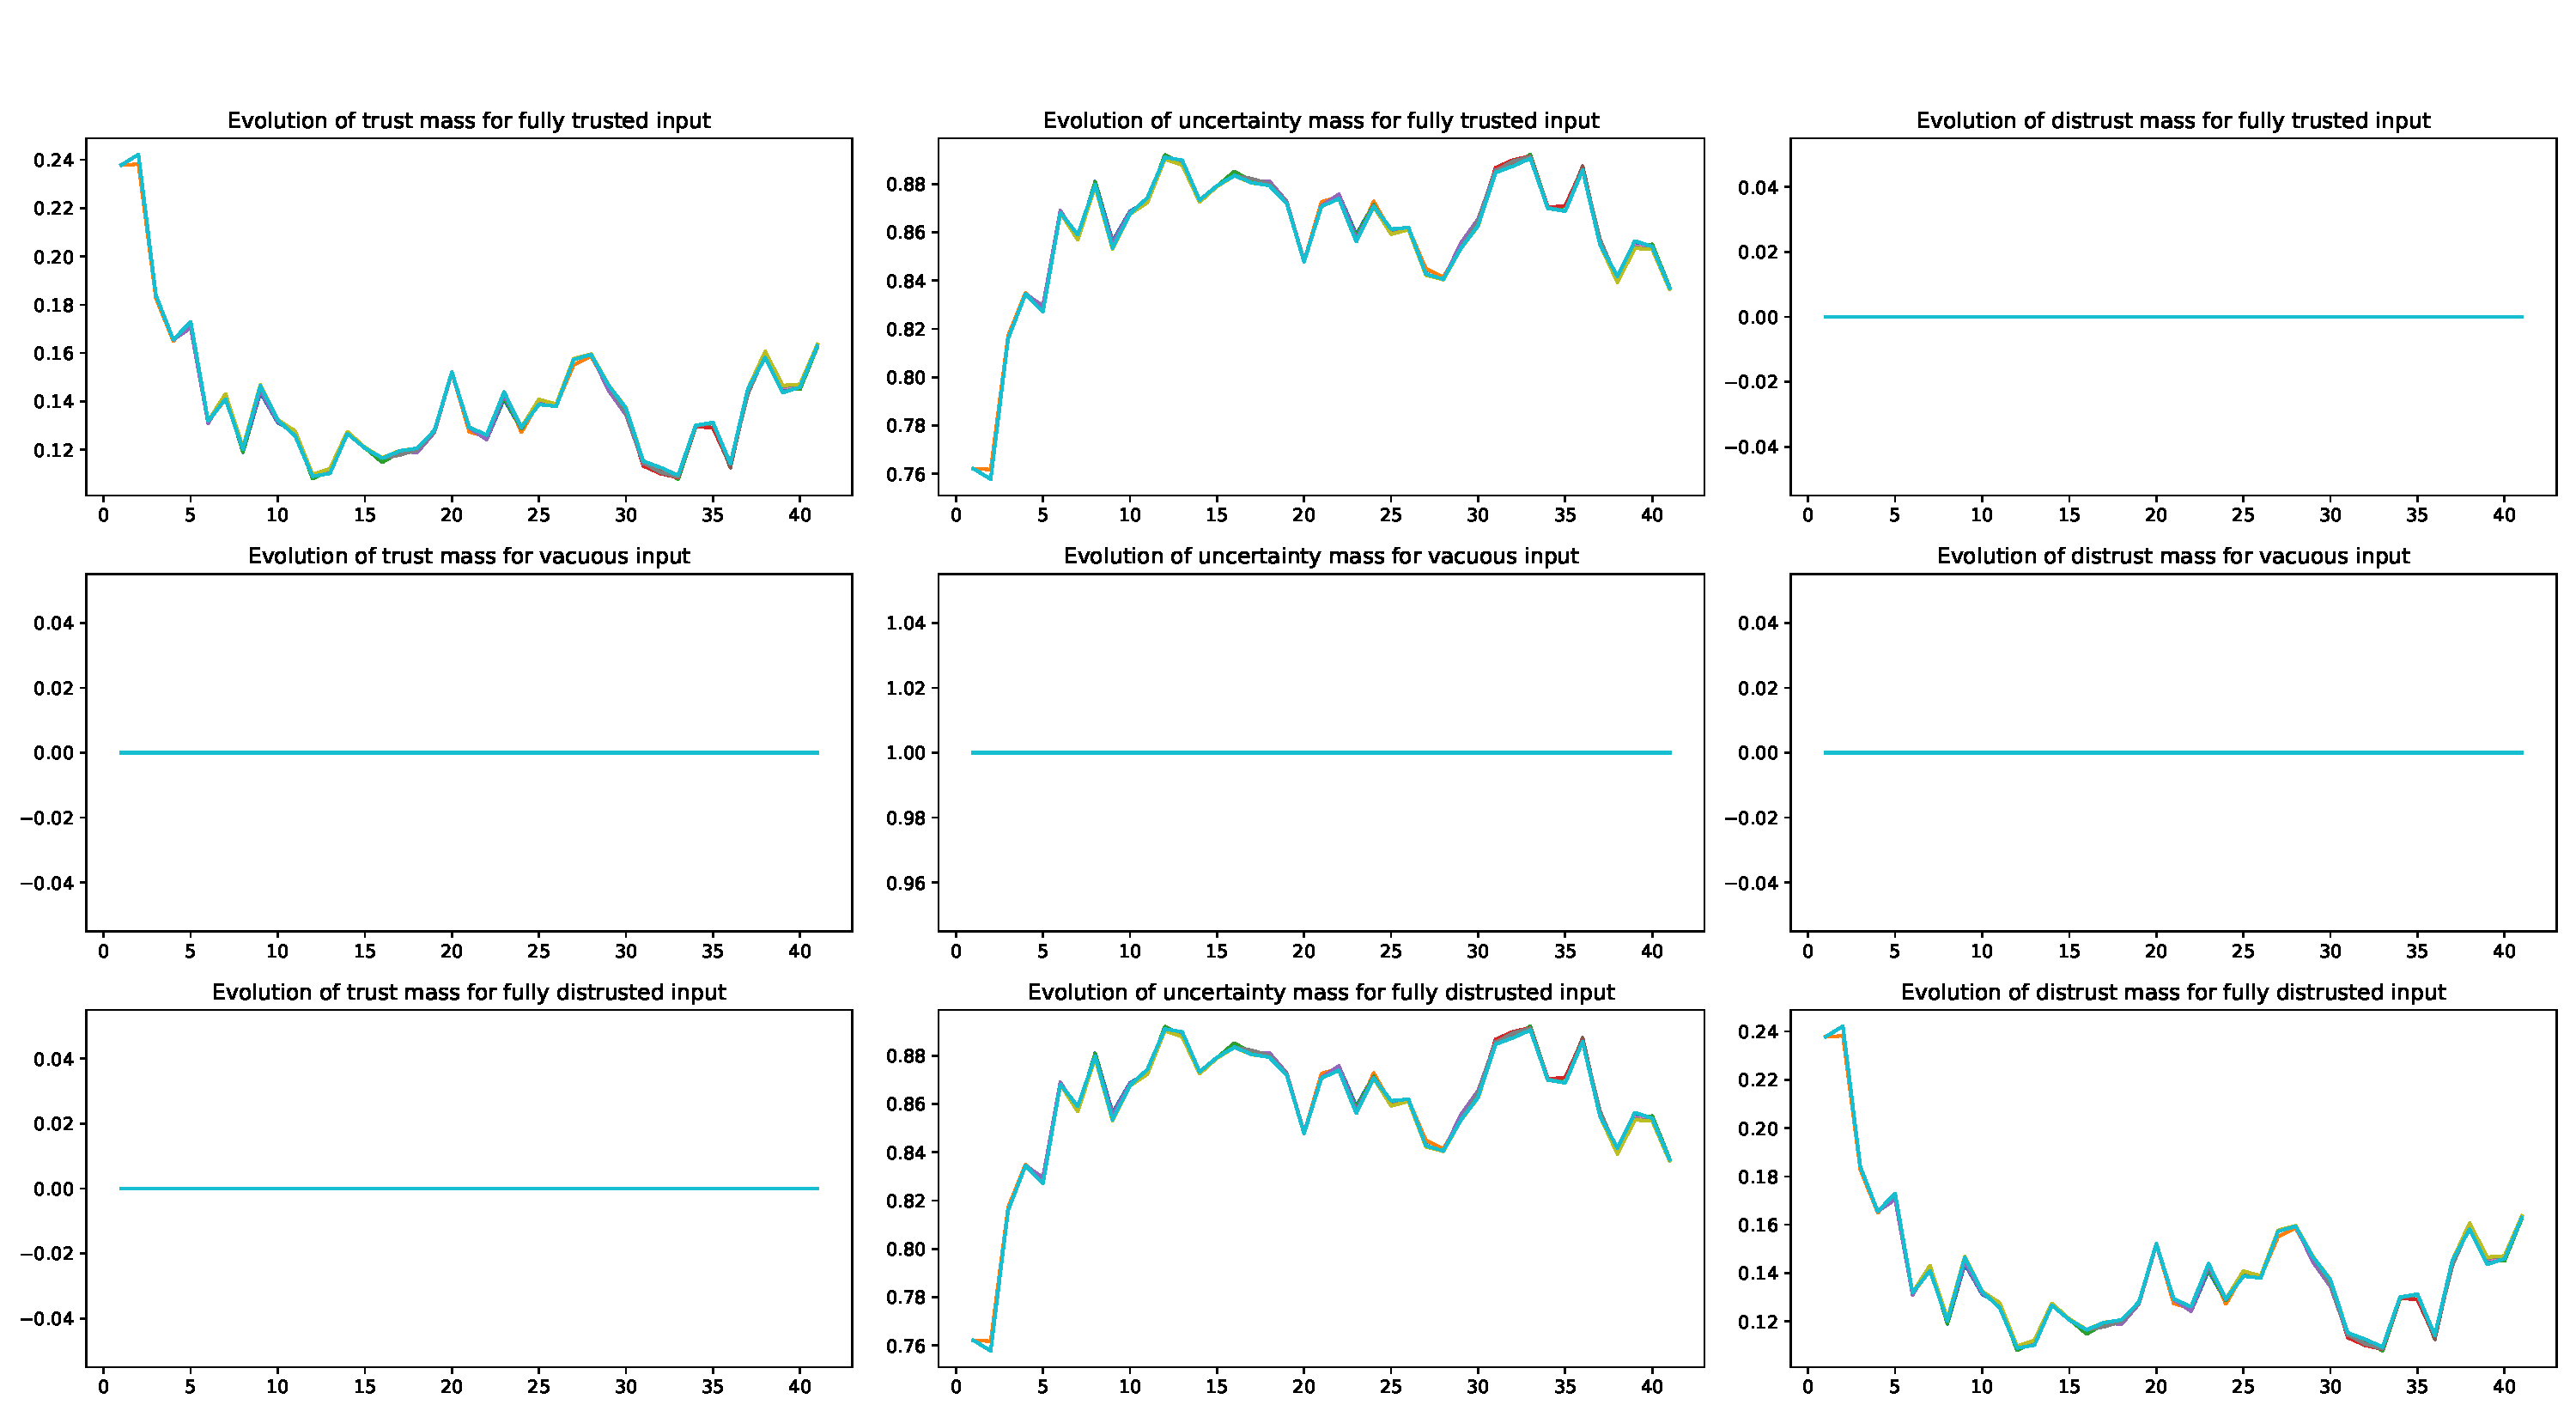
\includegraphics[width=\textwidth]{plots_v2/randomMNIST/all.pdf}
\caption{MNIST randomized trust}
\label{fig:mnistrand}
\end{figure}



% \subsection{Plots for Cancer Model with \(\epsilon = 0.01\) (\cref{exp:1})}\label{sec:rescancer0.01}
\begin{figure}[H]
  \includegraphics[width=\textwidth]{plots_v2/Cancer/eps=0.01/plot_ptas-d-d.pdf}
  \caption{Features distrusted and labels distrusted}
\end{figure}
\begin{figure}[H]
  \includegraphics[width=\textwidth]{plots_v2/Cancer/eps=0.01/plot_ptas-d-v.pdf}
  \caption{Features distrusted and labels vacuous}
\end{figure}
\begin{figure}[H]
  \includegraphics[width=\textwidth]{plots_v2/Cancer/eps=0.01/plot_ptas-d-t.pdf}
  \caption{Features distrusted and labels trusted}
\end{figure}
\begin{figure}[H]
  \includegraphics[width=\textwidth]{plots_v2/Cancer/eps=0.01/plot_ptas-v-d.pdf}
  \caption{Features vacuous and labels distrusted}
\end{figure}
\begin{figure}[H]
  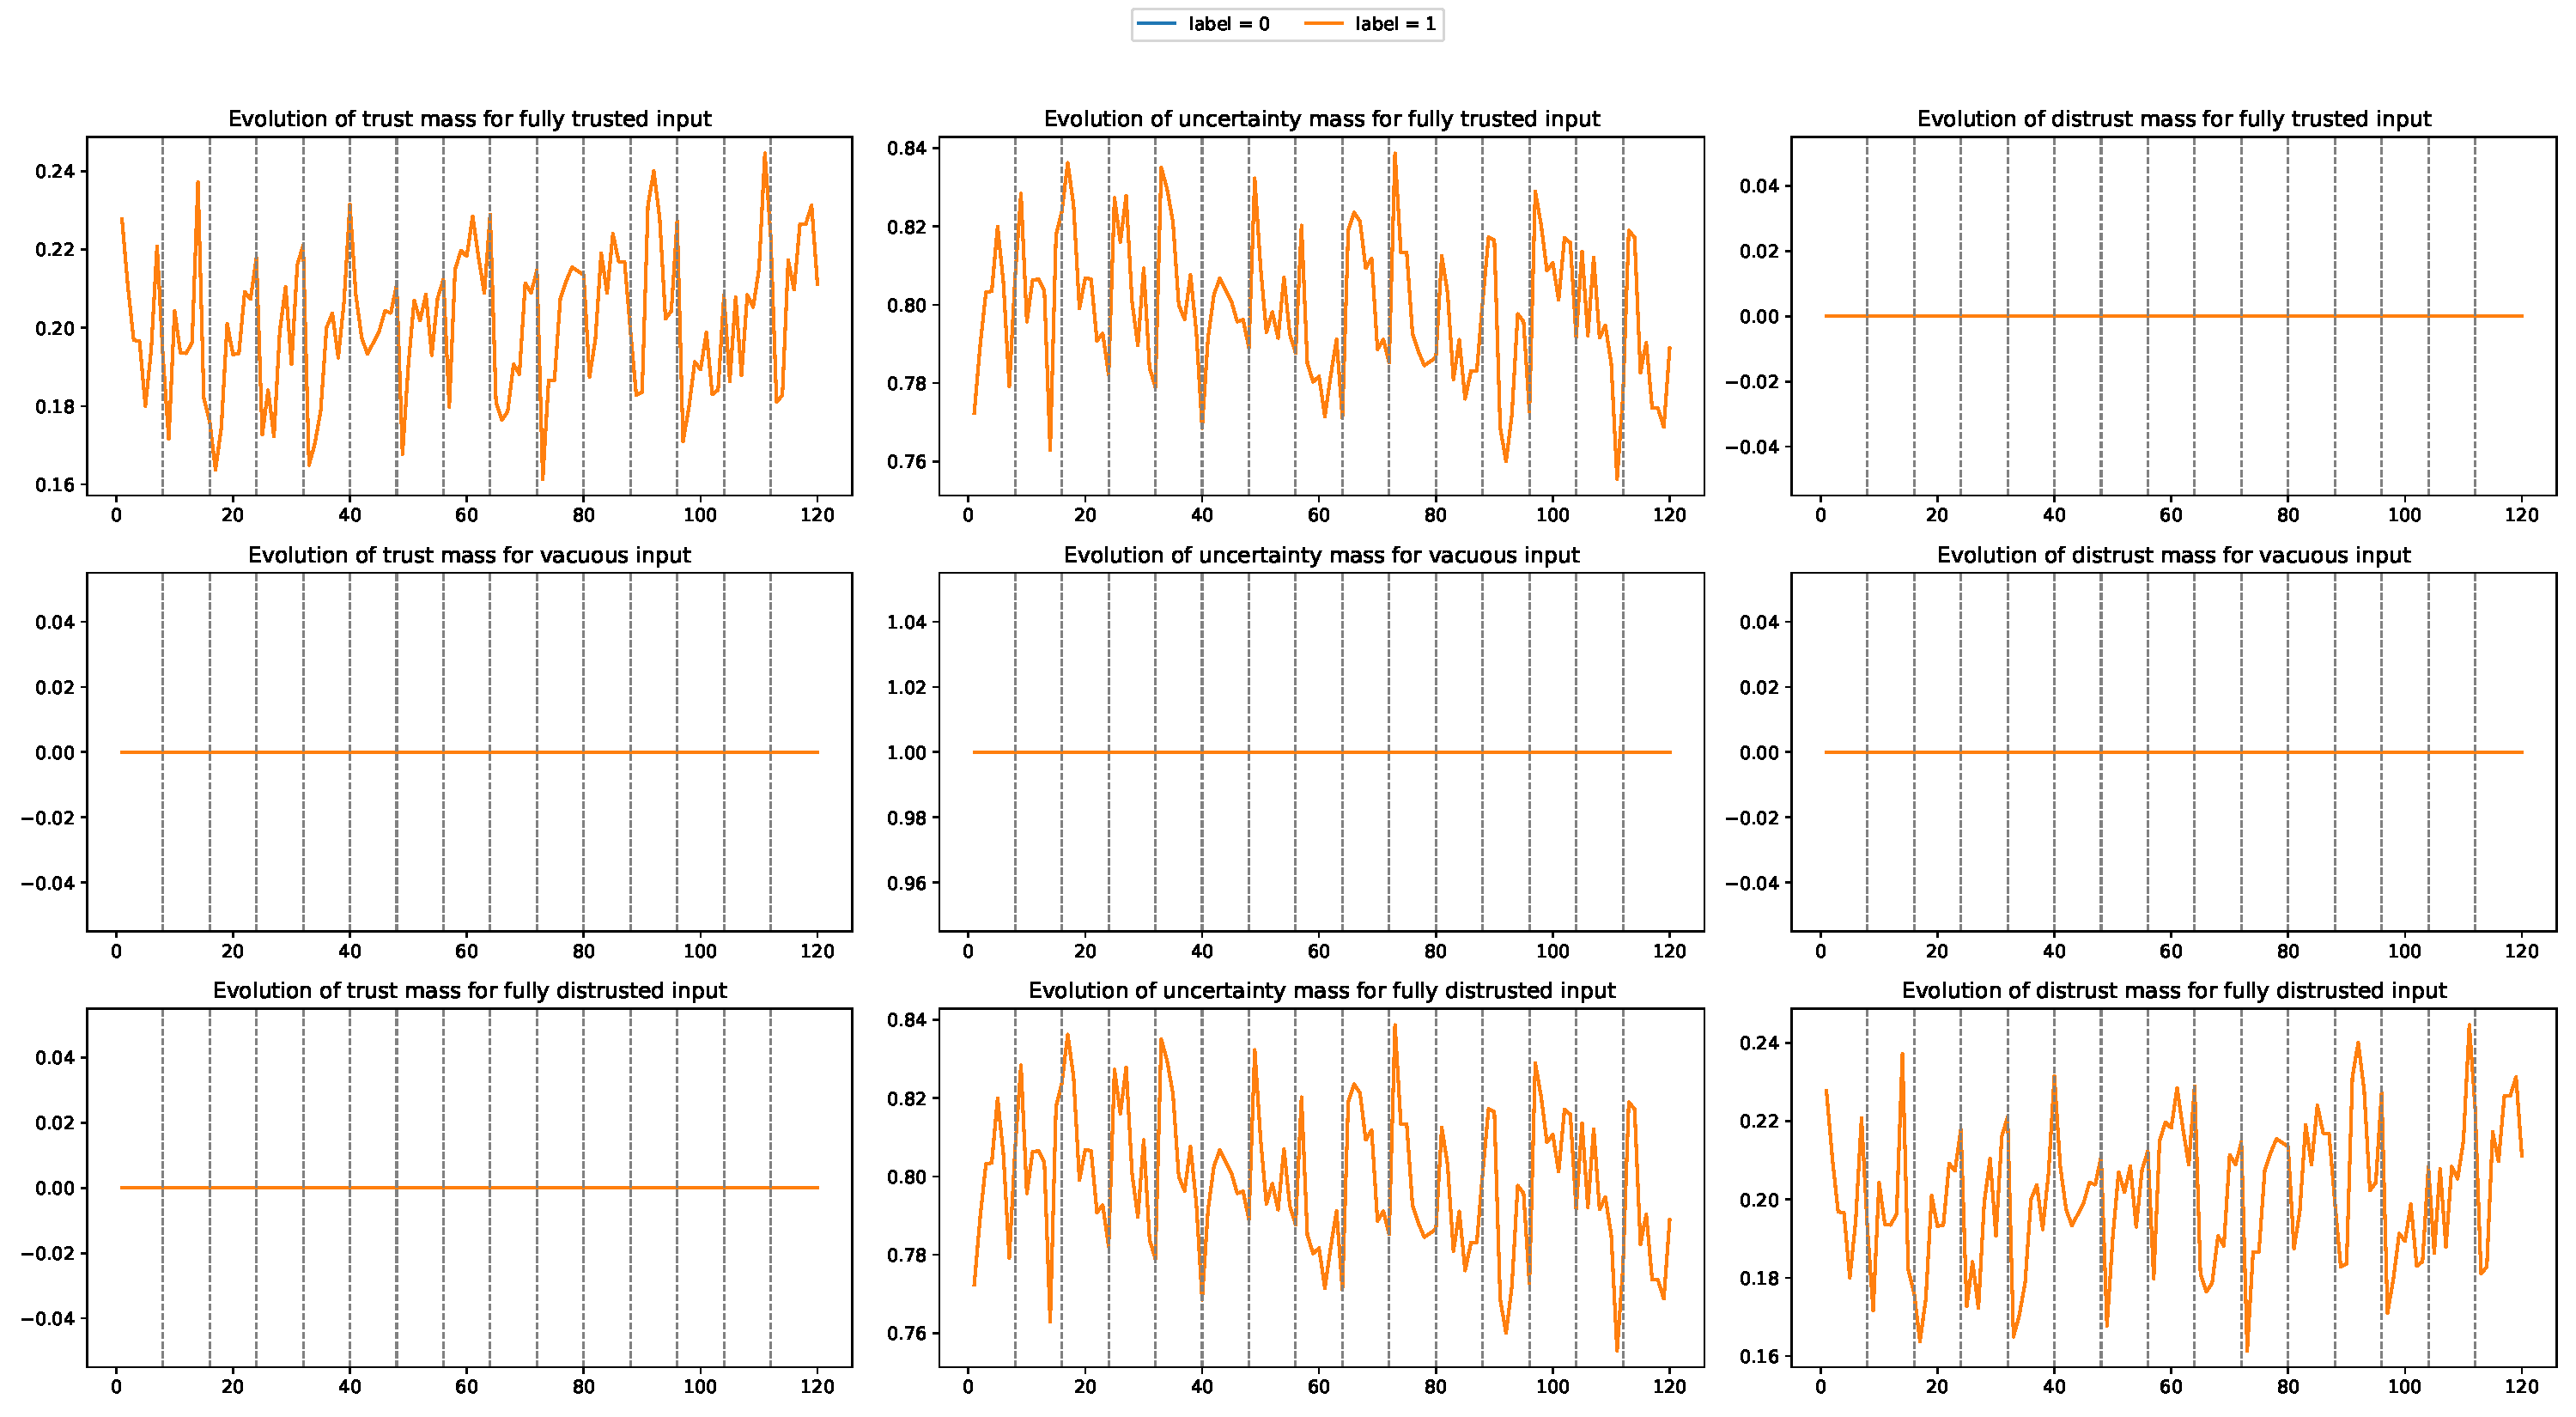
\includegraphics[width=\textwidth]{plots_v2/Cancer/eps=0.01/plot_ptas-v-v.pdf}
  \caption{Features vacuous and labels vacuous}
\end{figure}
\begin{figure}[H]
  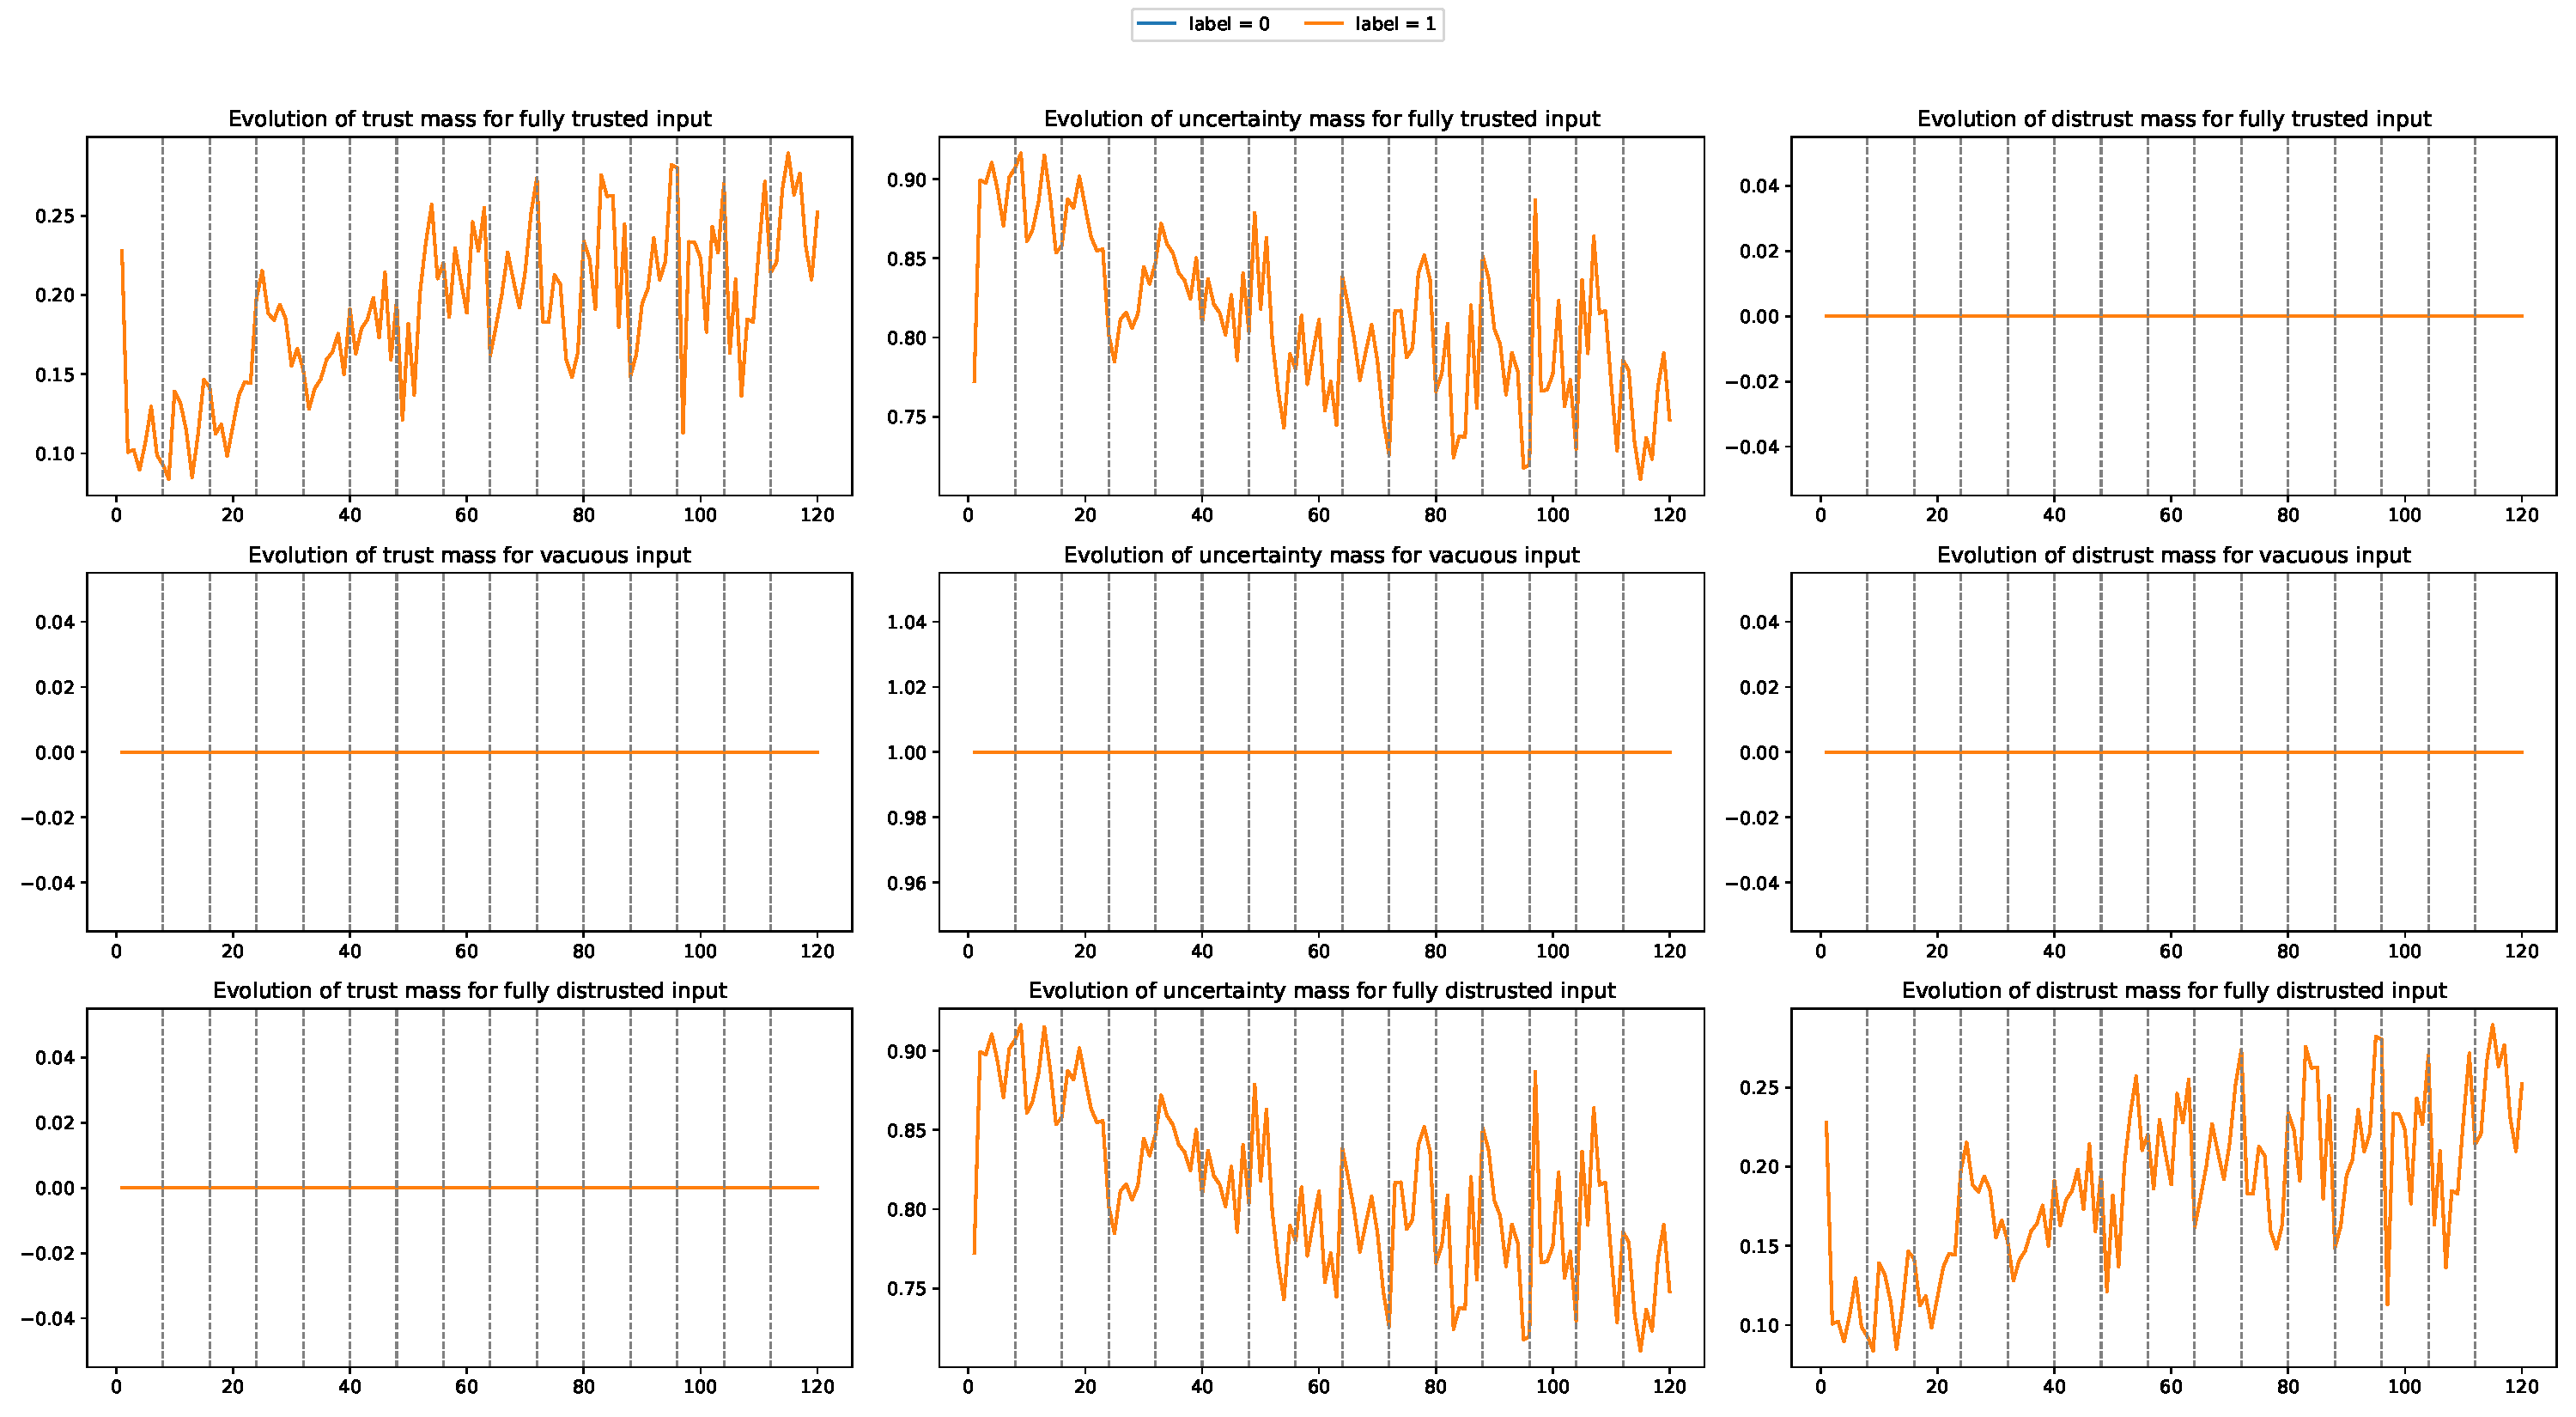
\includegraphics[width=\textwidth]{plots_v2/Cancer/eps=0.01/plot_ptas-v-t.pdf}
  \caption{Features vacuous and labels trusted}
\end{figure}
\begin{figure}[H]
  \includegraphics[width=\textwidth]{plots_v2/Cancer/eps=0.01/plot_ptas-t-d.pdf}
  \caption{Features trusted and labels distrusted}
\end{figure}
\begin{figure}[H]
  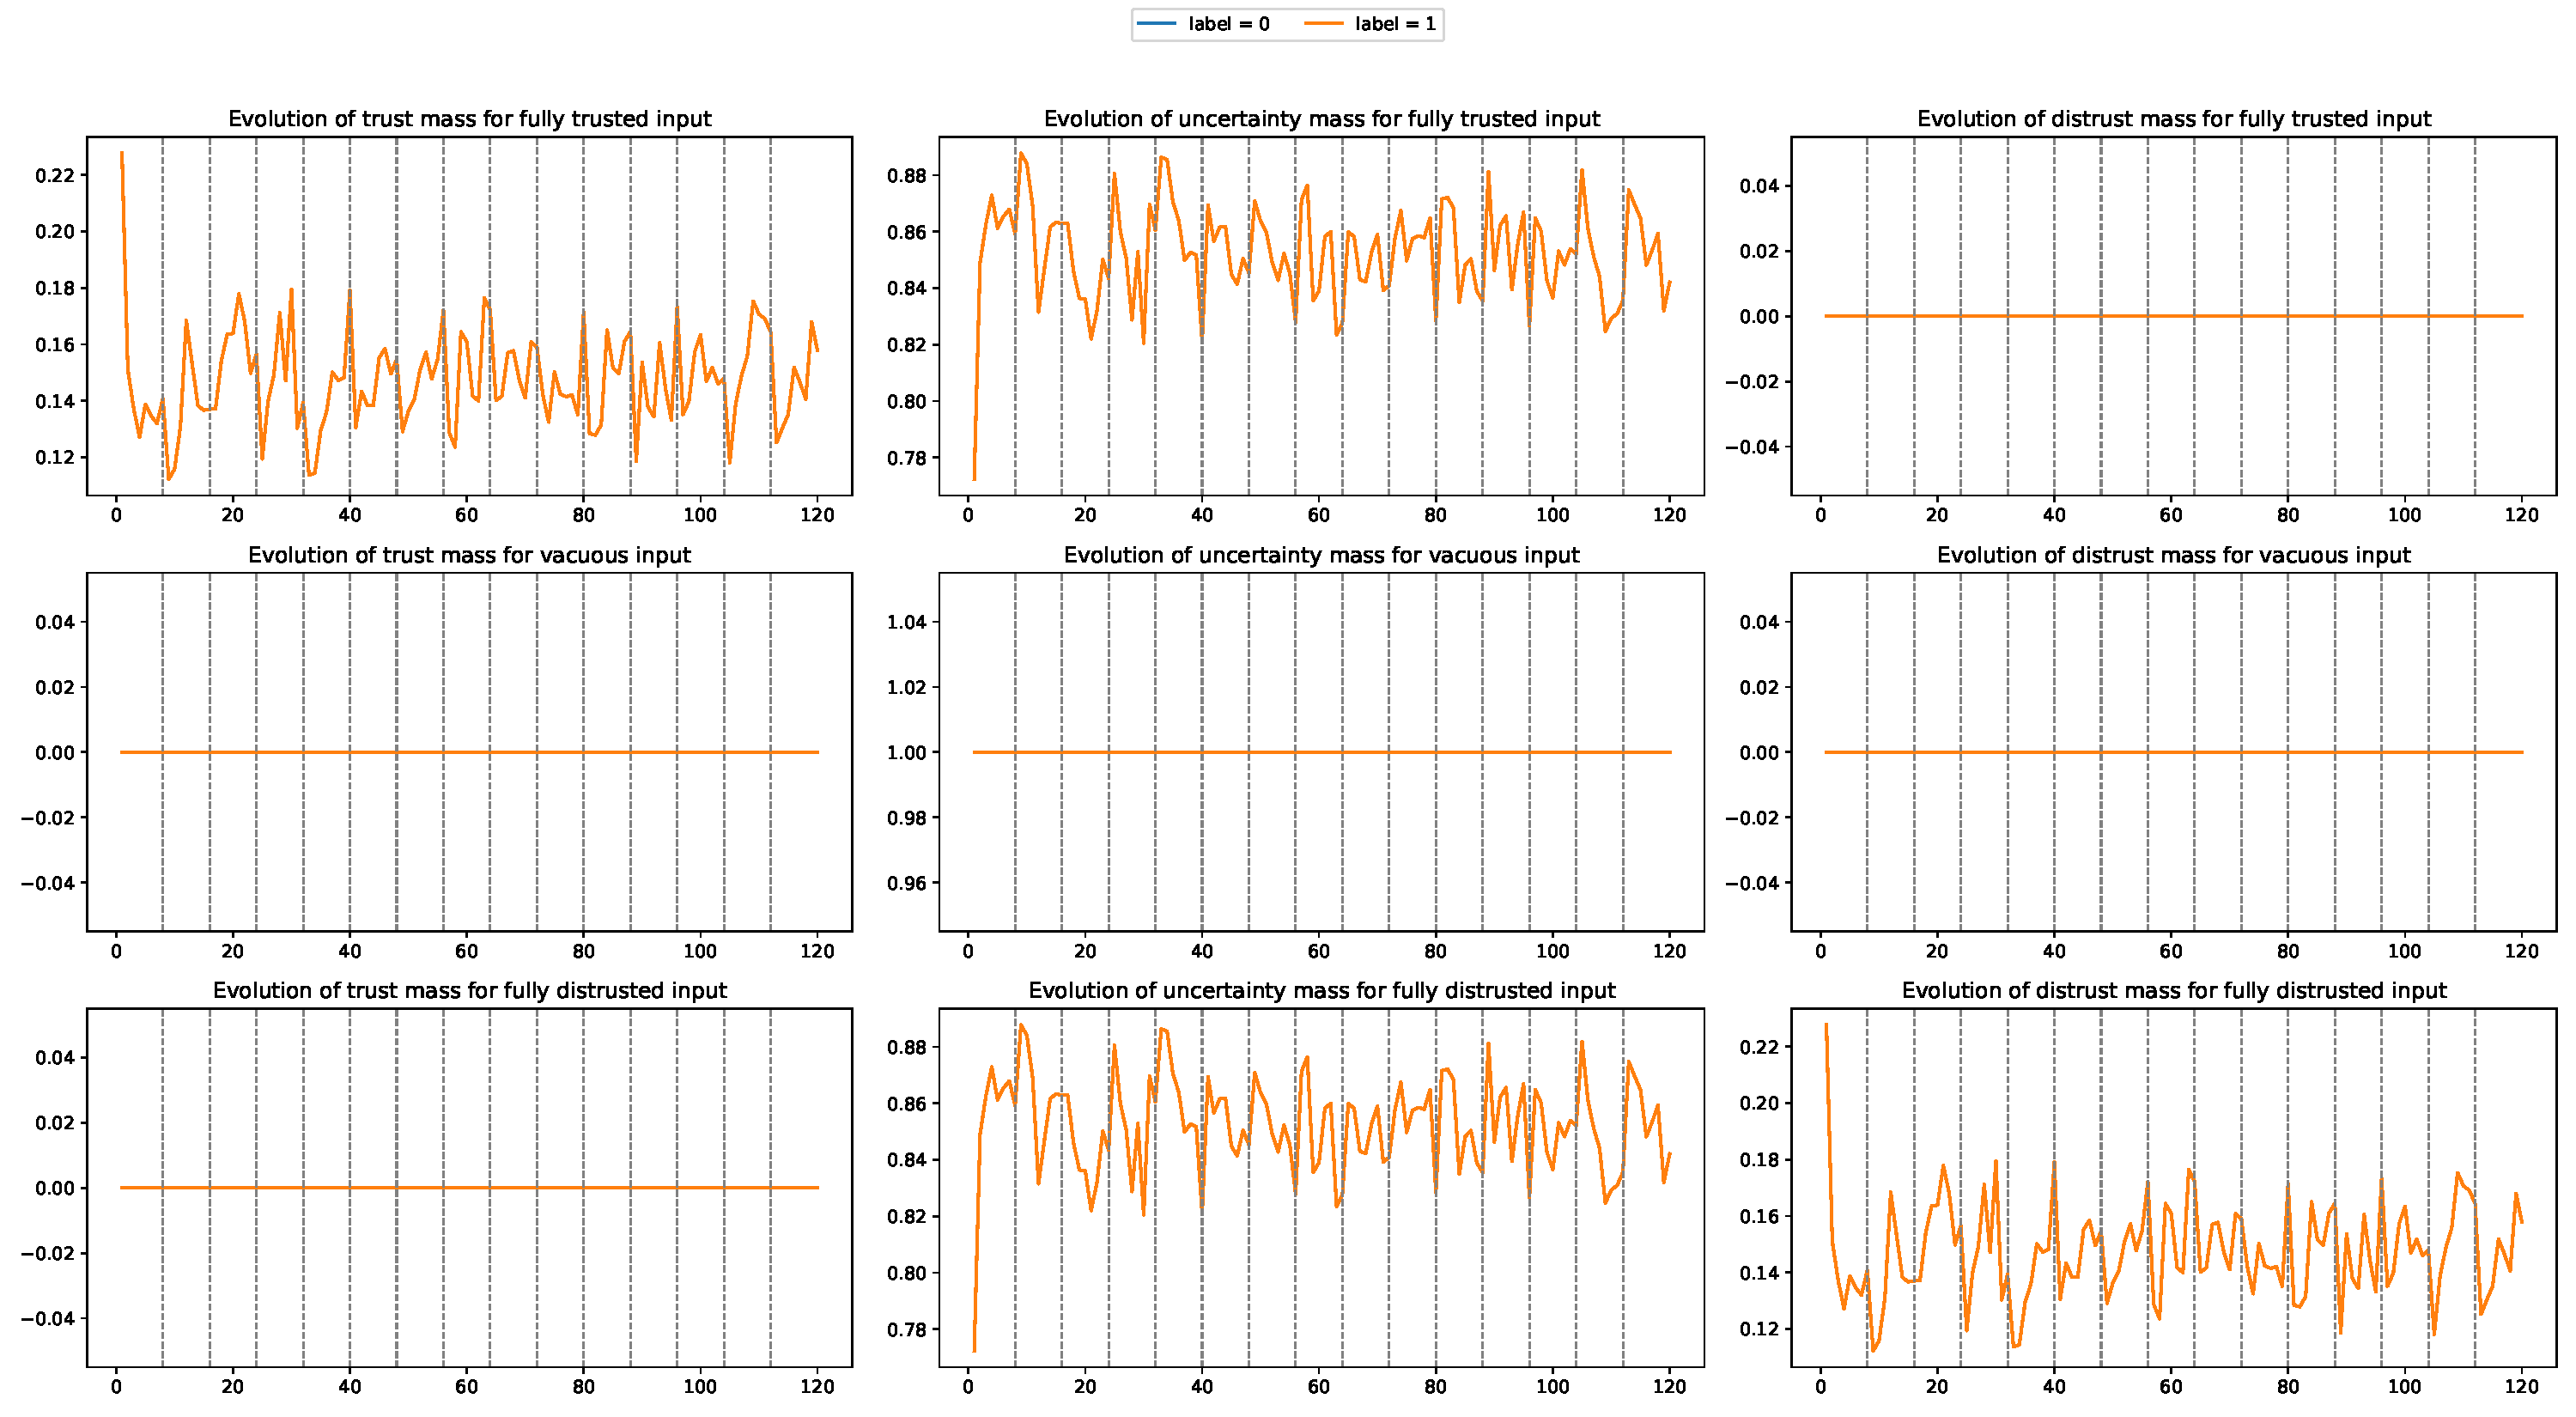
\includegraphics[width=\textwidth]{plots_v2/Cancer/eps=0.01/plot_ptas-t-v.pdf}
  \caption{Features trusted and labels vacuous}
\end{figure}
\begin{figure}[H]
  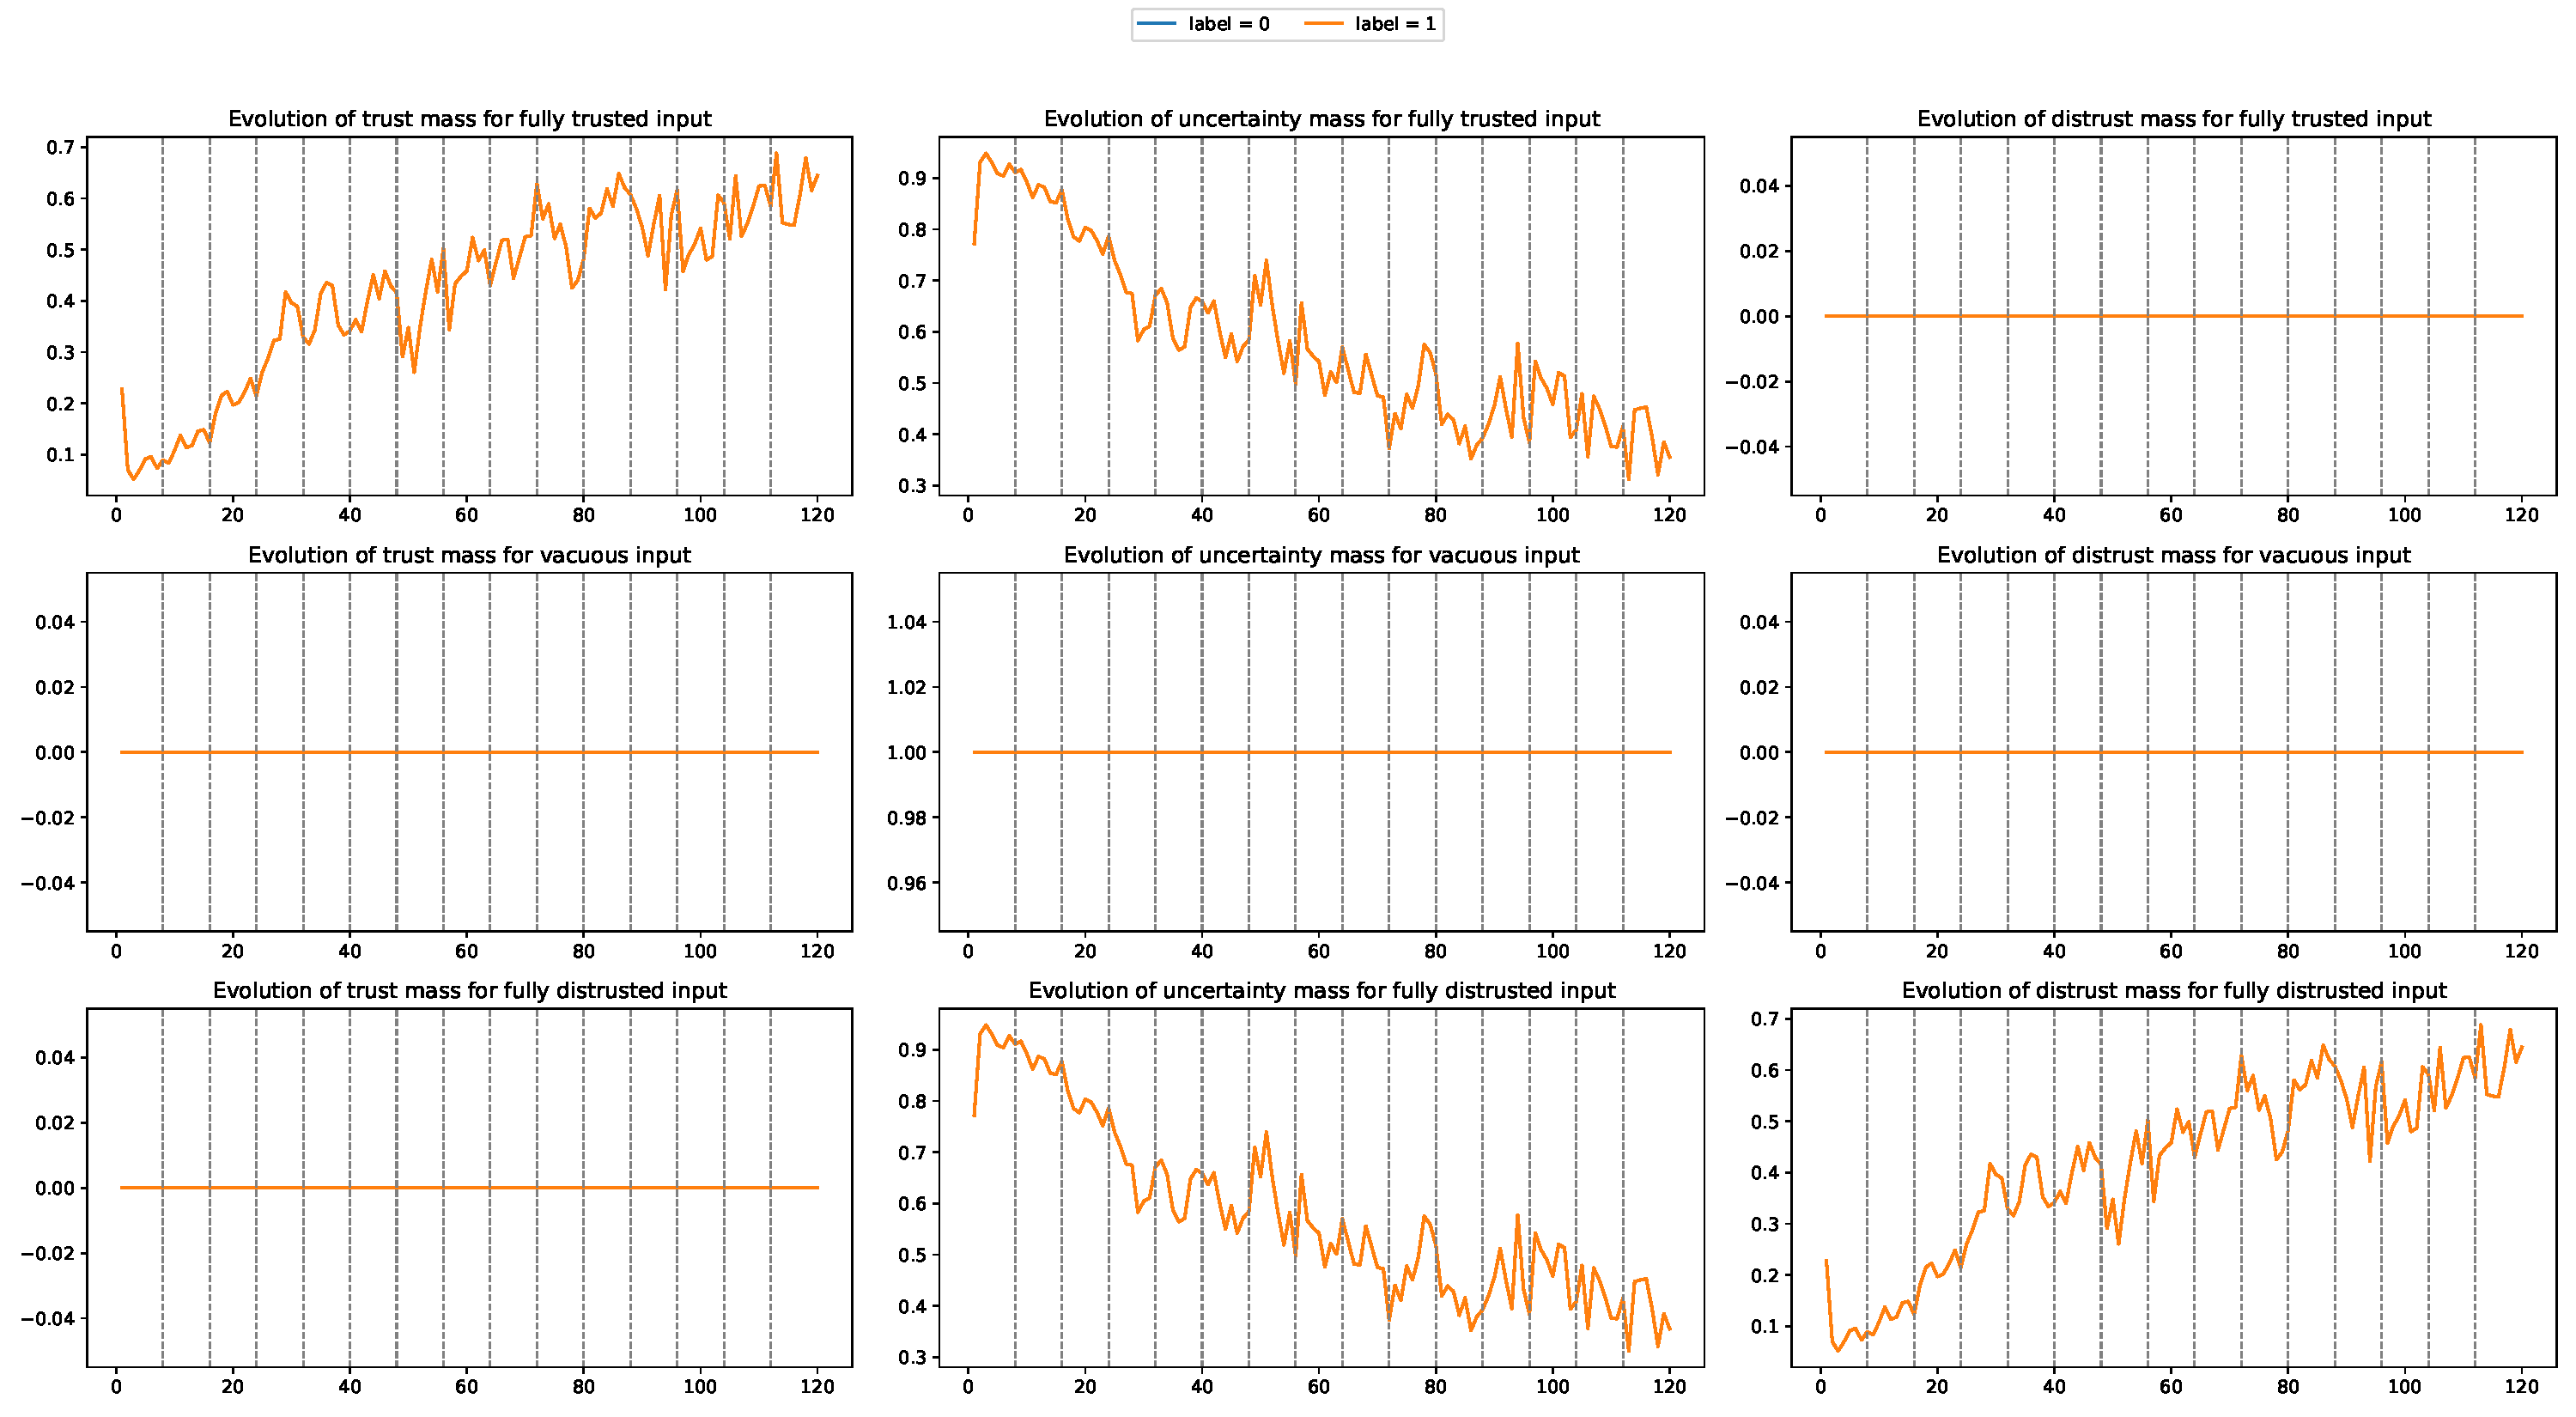
\includegraphics[width=\textwidth]{plots_v2/Cancer/eps=0.01/plot_ptas-t-t.pdf}
  \caption{Features trusted and labels trusted}
\end{figure}

\subsection{Cancer Model with \( \epsilon = 0.1 \)(\cref{exp:1})}\label{sec:rescancer0.1}
\begin{figure}[H]
  \includegraphics[width=\textwidth]{plots_v2/Cancer/eps=0.1/plot_ptas-d-d.pdf}
  \caption{Features distrusted and labels distrusted}
\end{figure}
\begin{figure}[H]
  \includegraphics[width=\textwidth]{plots_v2/Cancer/eps=0.1/plot_ptas-d-v.pdf}
  \caption{Features distrusted and labels vacuous}
\end{figure}
\begin{figure}[H]
  \includegraphics[width=\textwidth]{plots_v2/Cancer/eps=0.1/plot_ptas-d-t.pdf}
  \caption{Features distrusted and labels trusted}
\end{figure}
\begin{figure}[H]
  \includegraphics[width=\textwidth]{plots_v2/Cancer/eps=0.1/plot_ptas-v-d.pdf}
  \caption{Features vacuous and labels distrusted}
\end{figure}
\begin{figure}[H]
  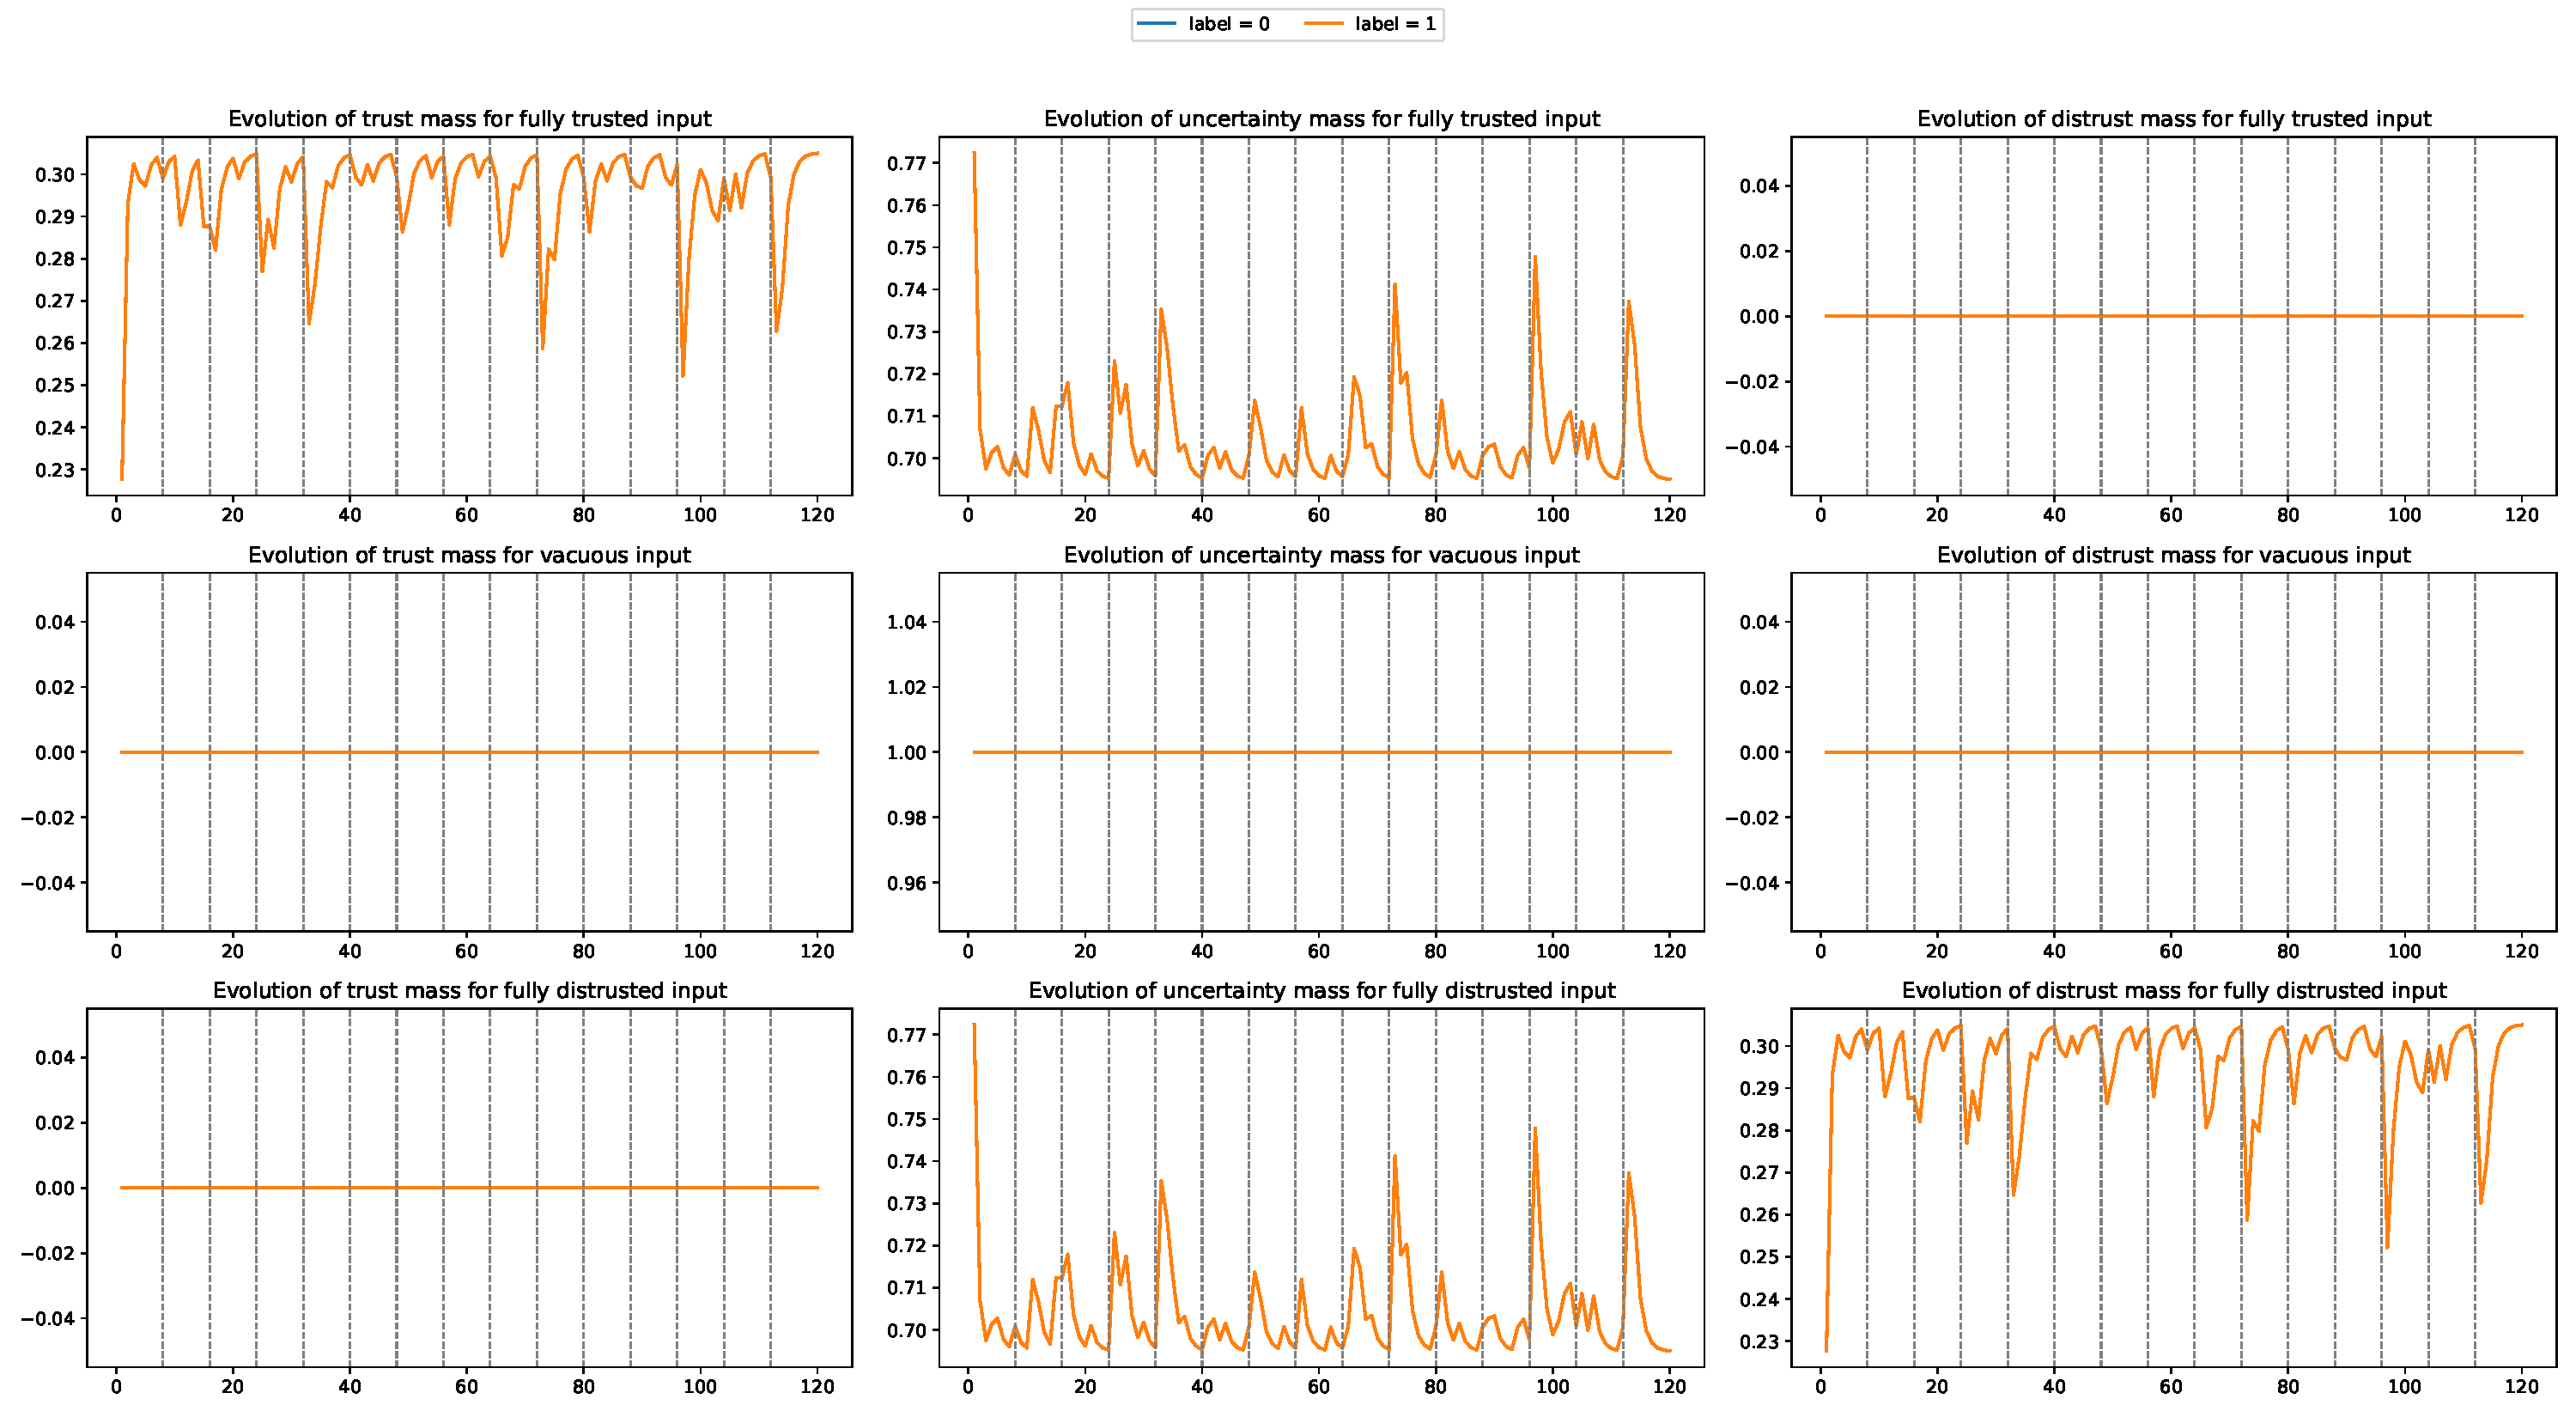
\includegraphics[width=\textwidth]{plots_v2/Cancer/eps=0.1/plot_ptas-v-v.pdf}
  \caption{Features vacuous and labels vacuous}
\end{figure}
\begin{figure}[H]
  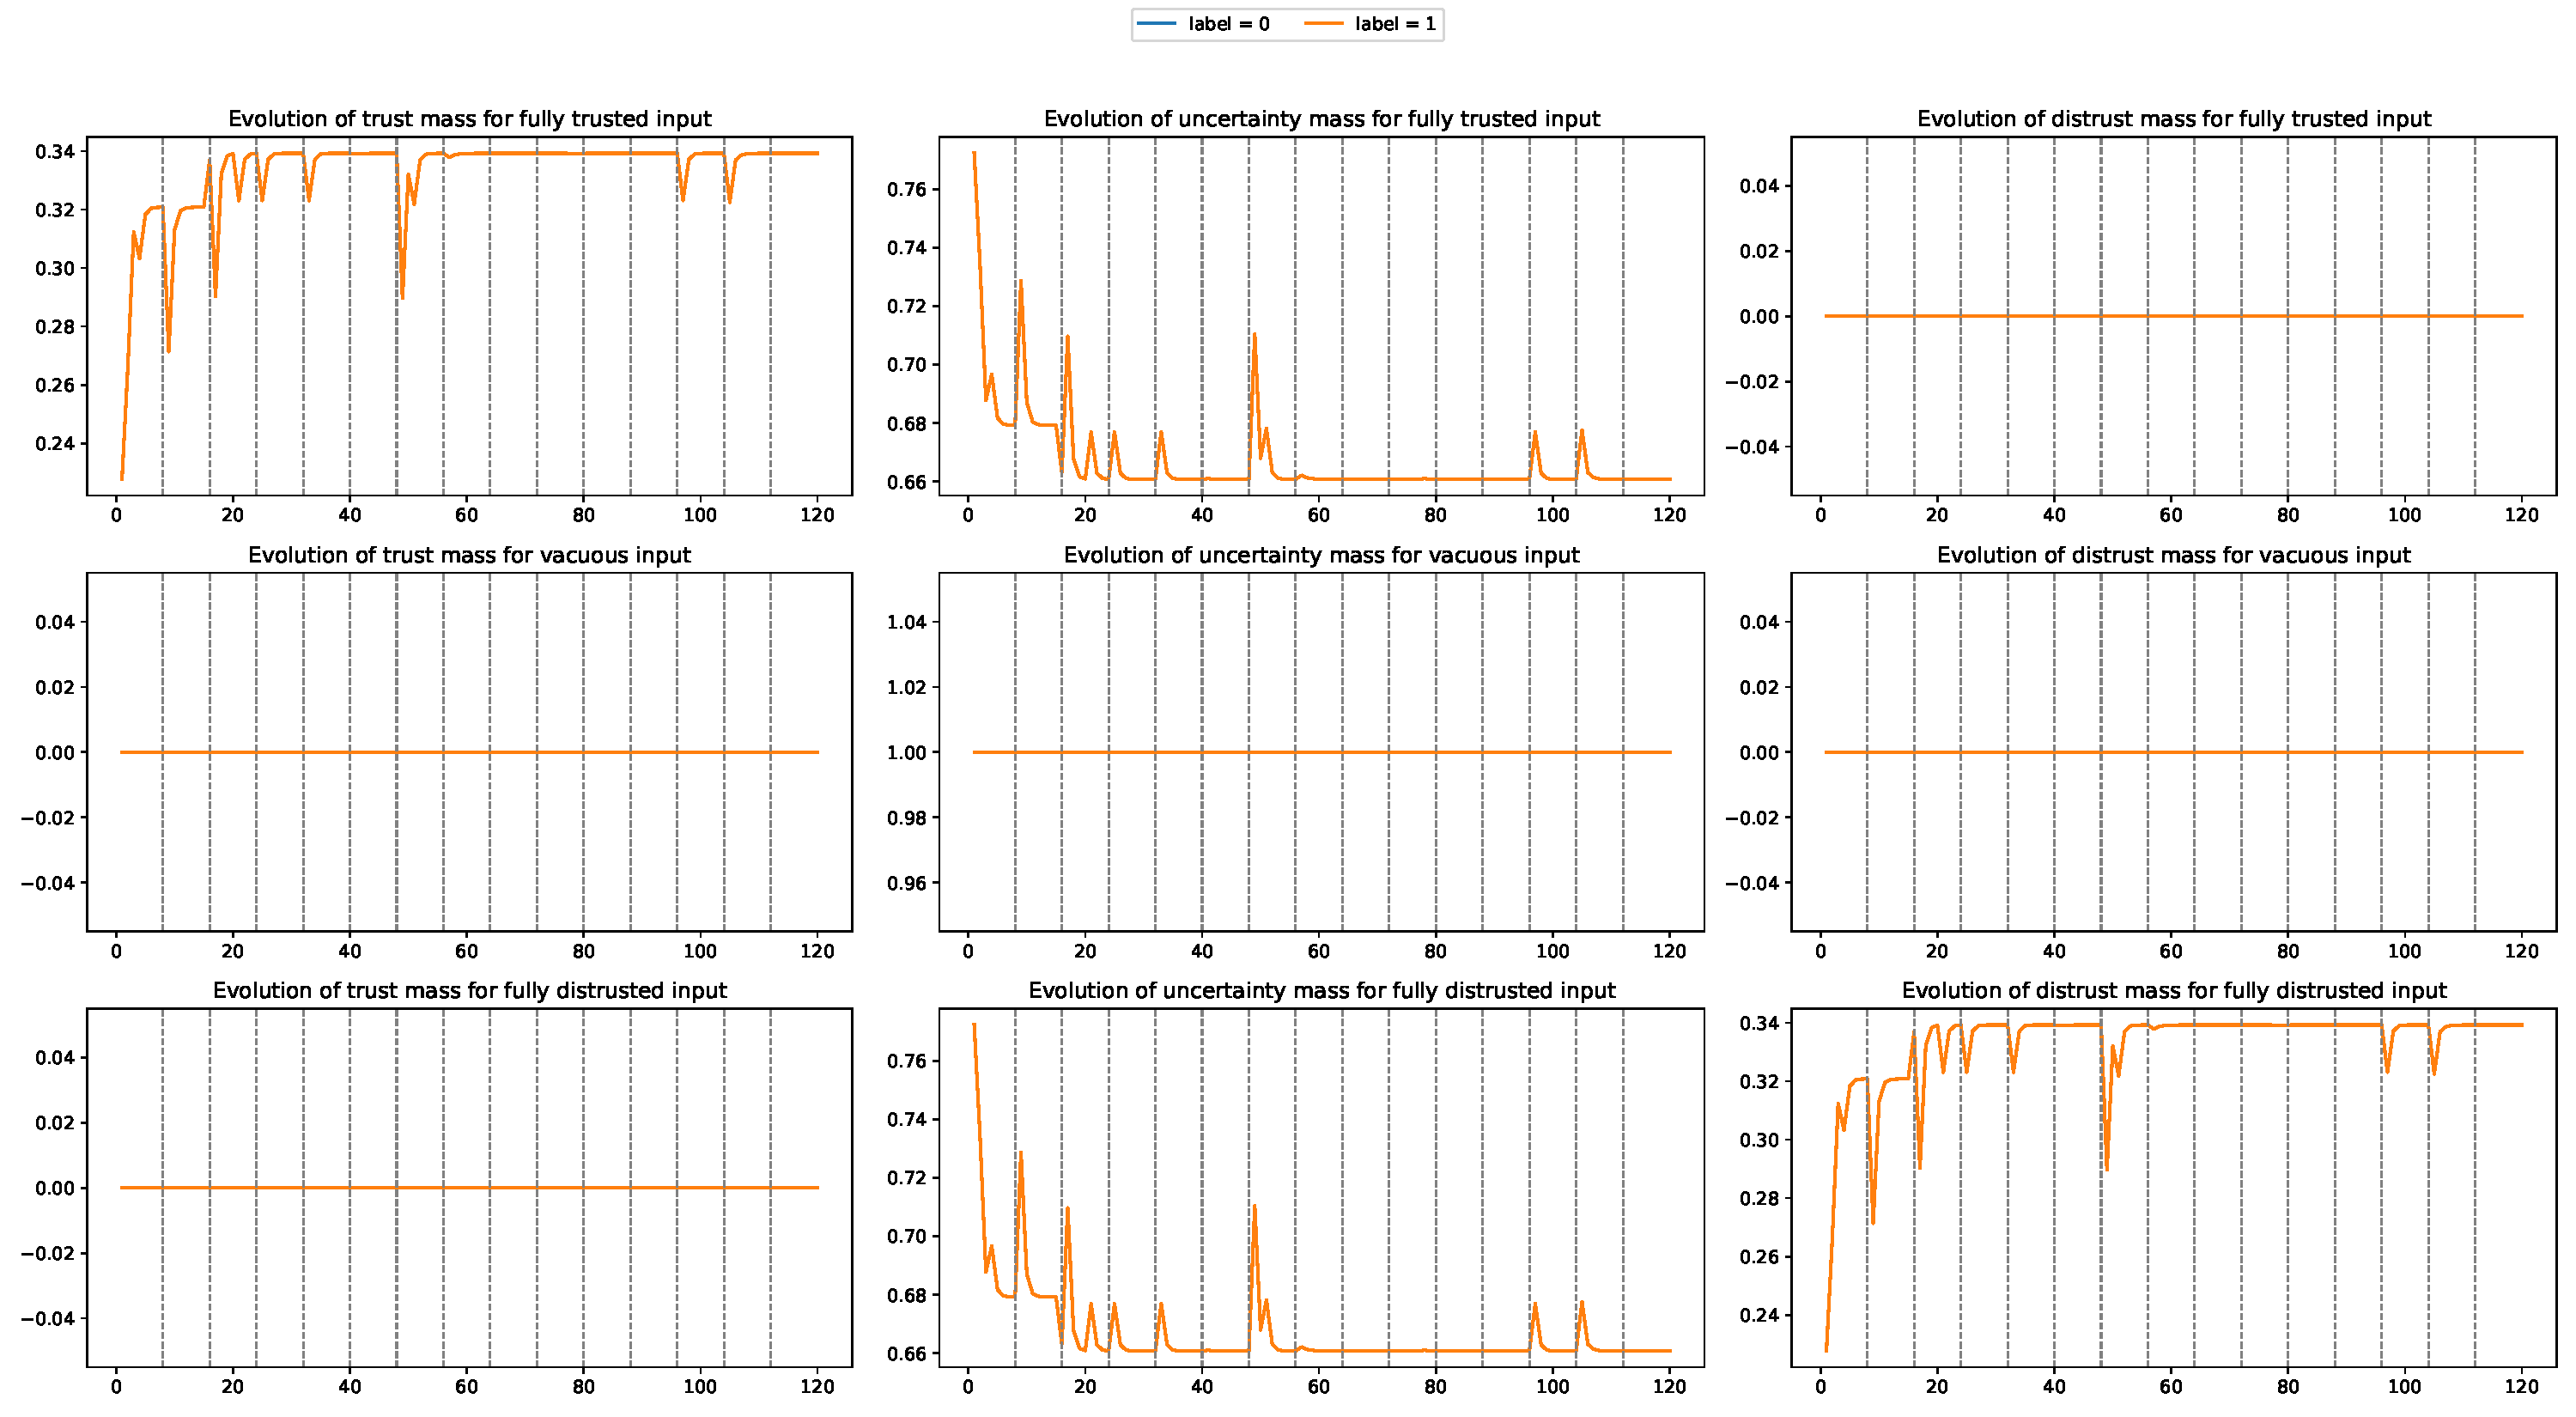
\includegraphics[width=\textwidth]{plots_v2/Cancer/eps=0.1/plot_ptas-v-t.pdf}
  \caption{Features vacuous and labels trusted}
\end{figure}
\begin{figure}[H]
  \includegraphics[width=\textwidth]{plots_v2/Cancer/eps=0.1/plot_ptas-t-d.pdf}
  \caption{Features trusted and labels distrusted}
\end{figure}
\begin{figure}[H]
  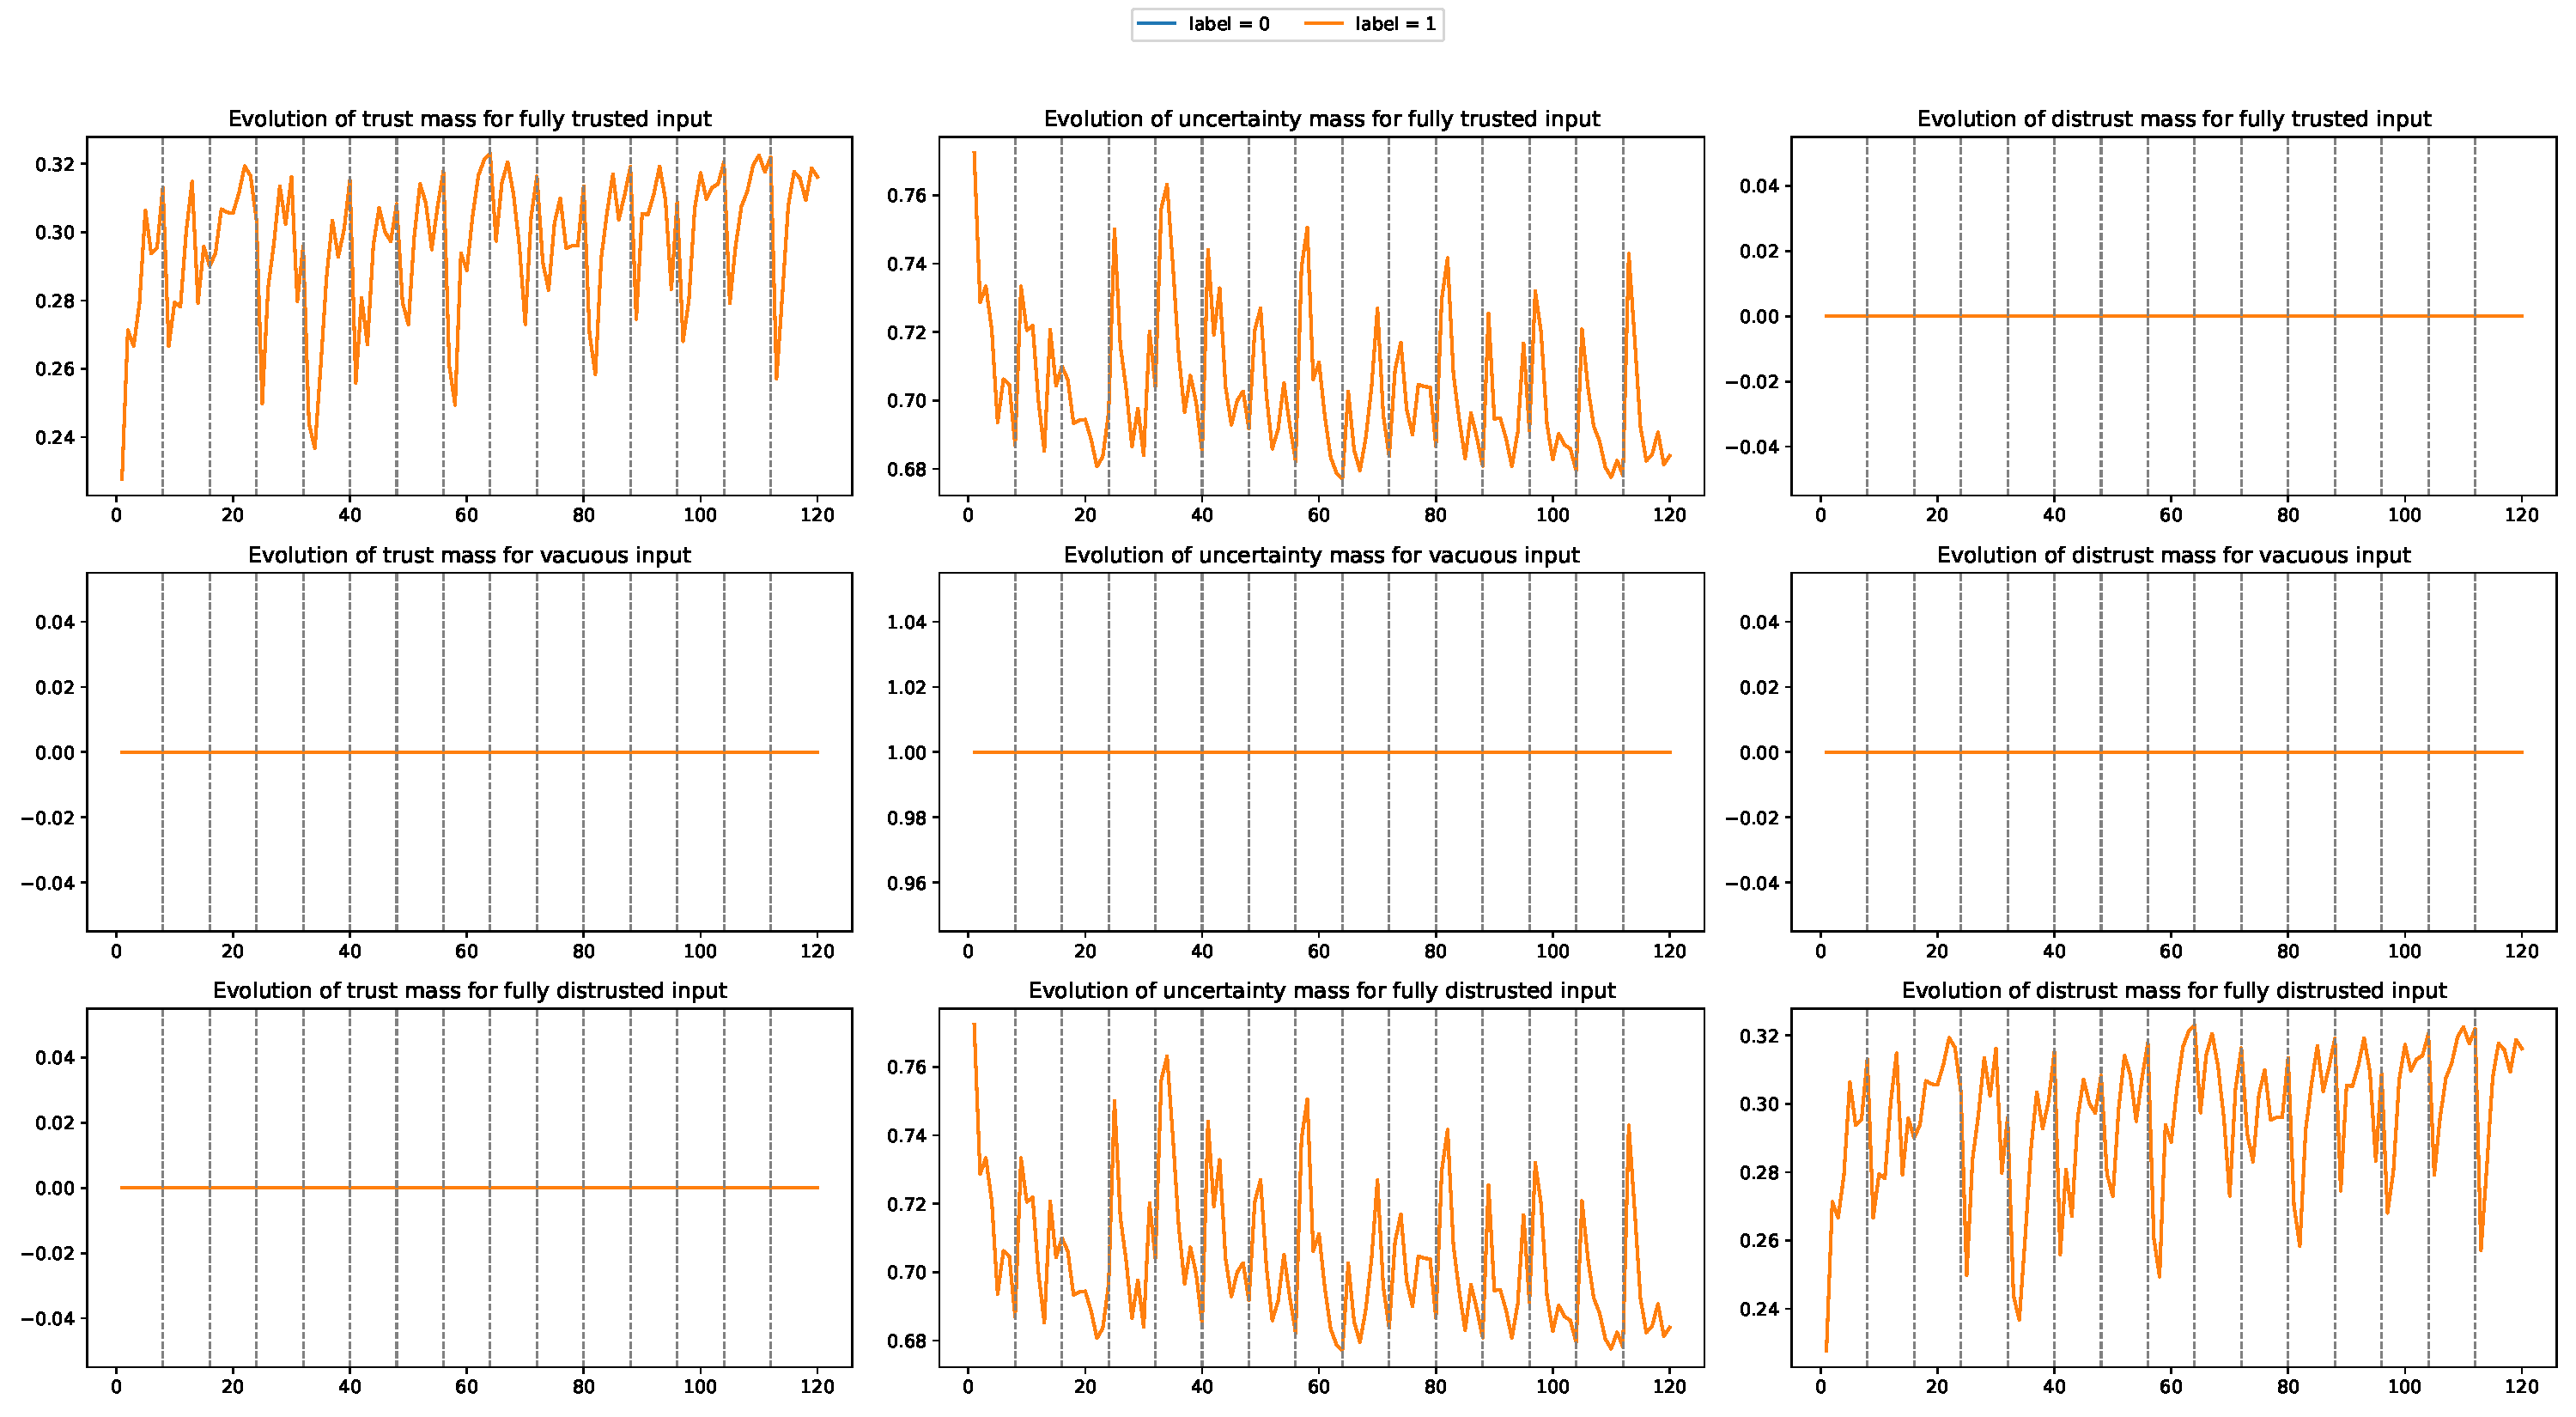
\includegraphics[width=\textwidth]{plots_v2/Cancer/eps=0.1/plot_ptas-t-v.pdf}
  \caption{Features trusted and labels vacuous}
\end{figure}
\begin{figure}[H]
  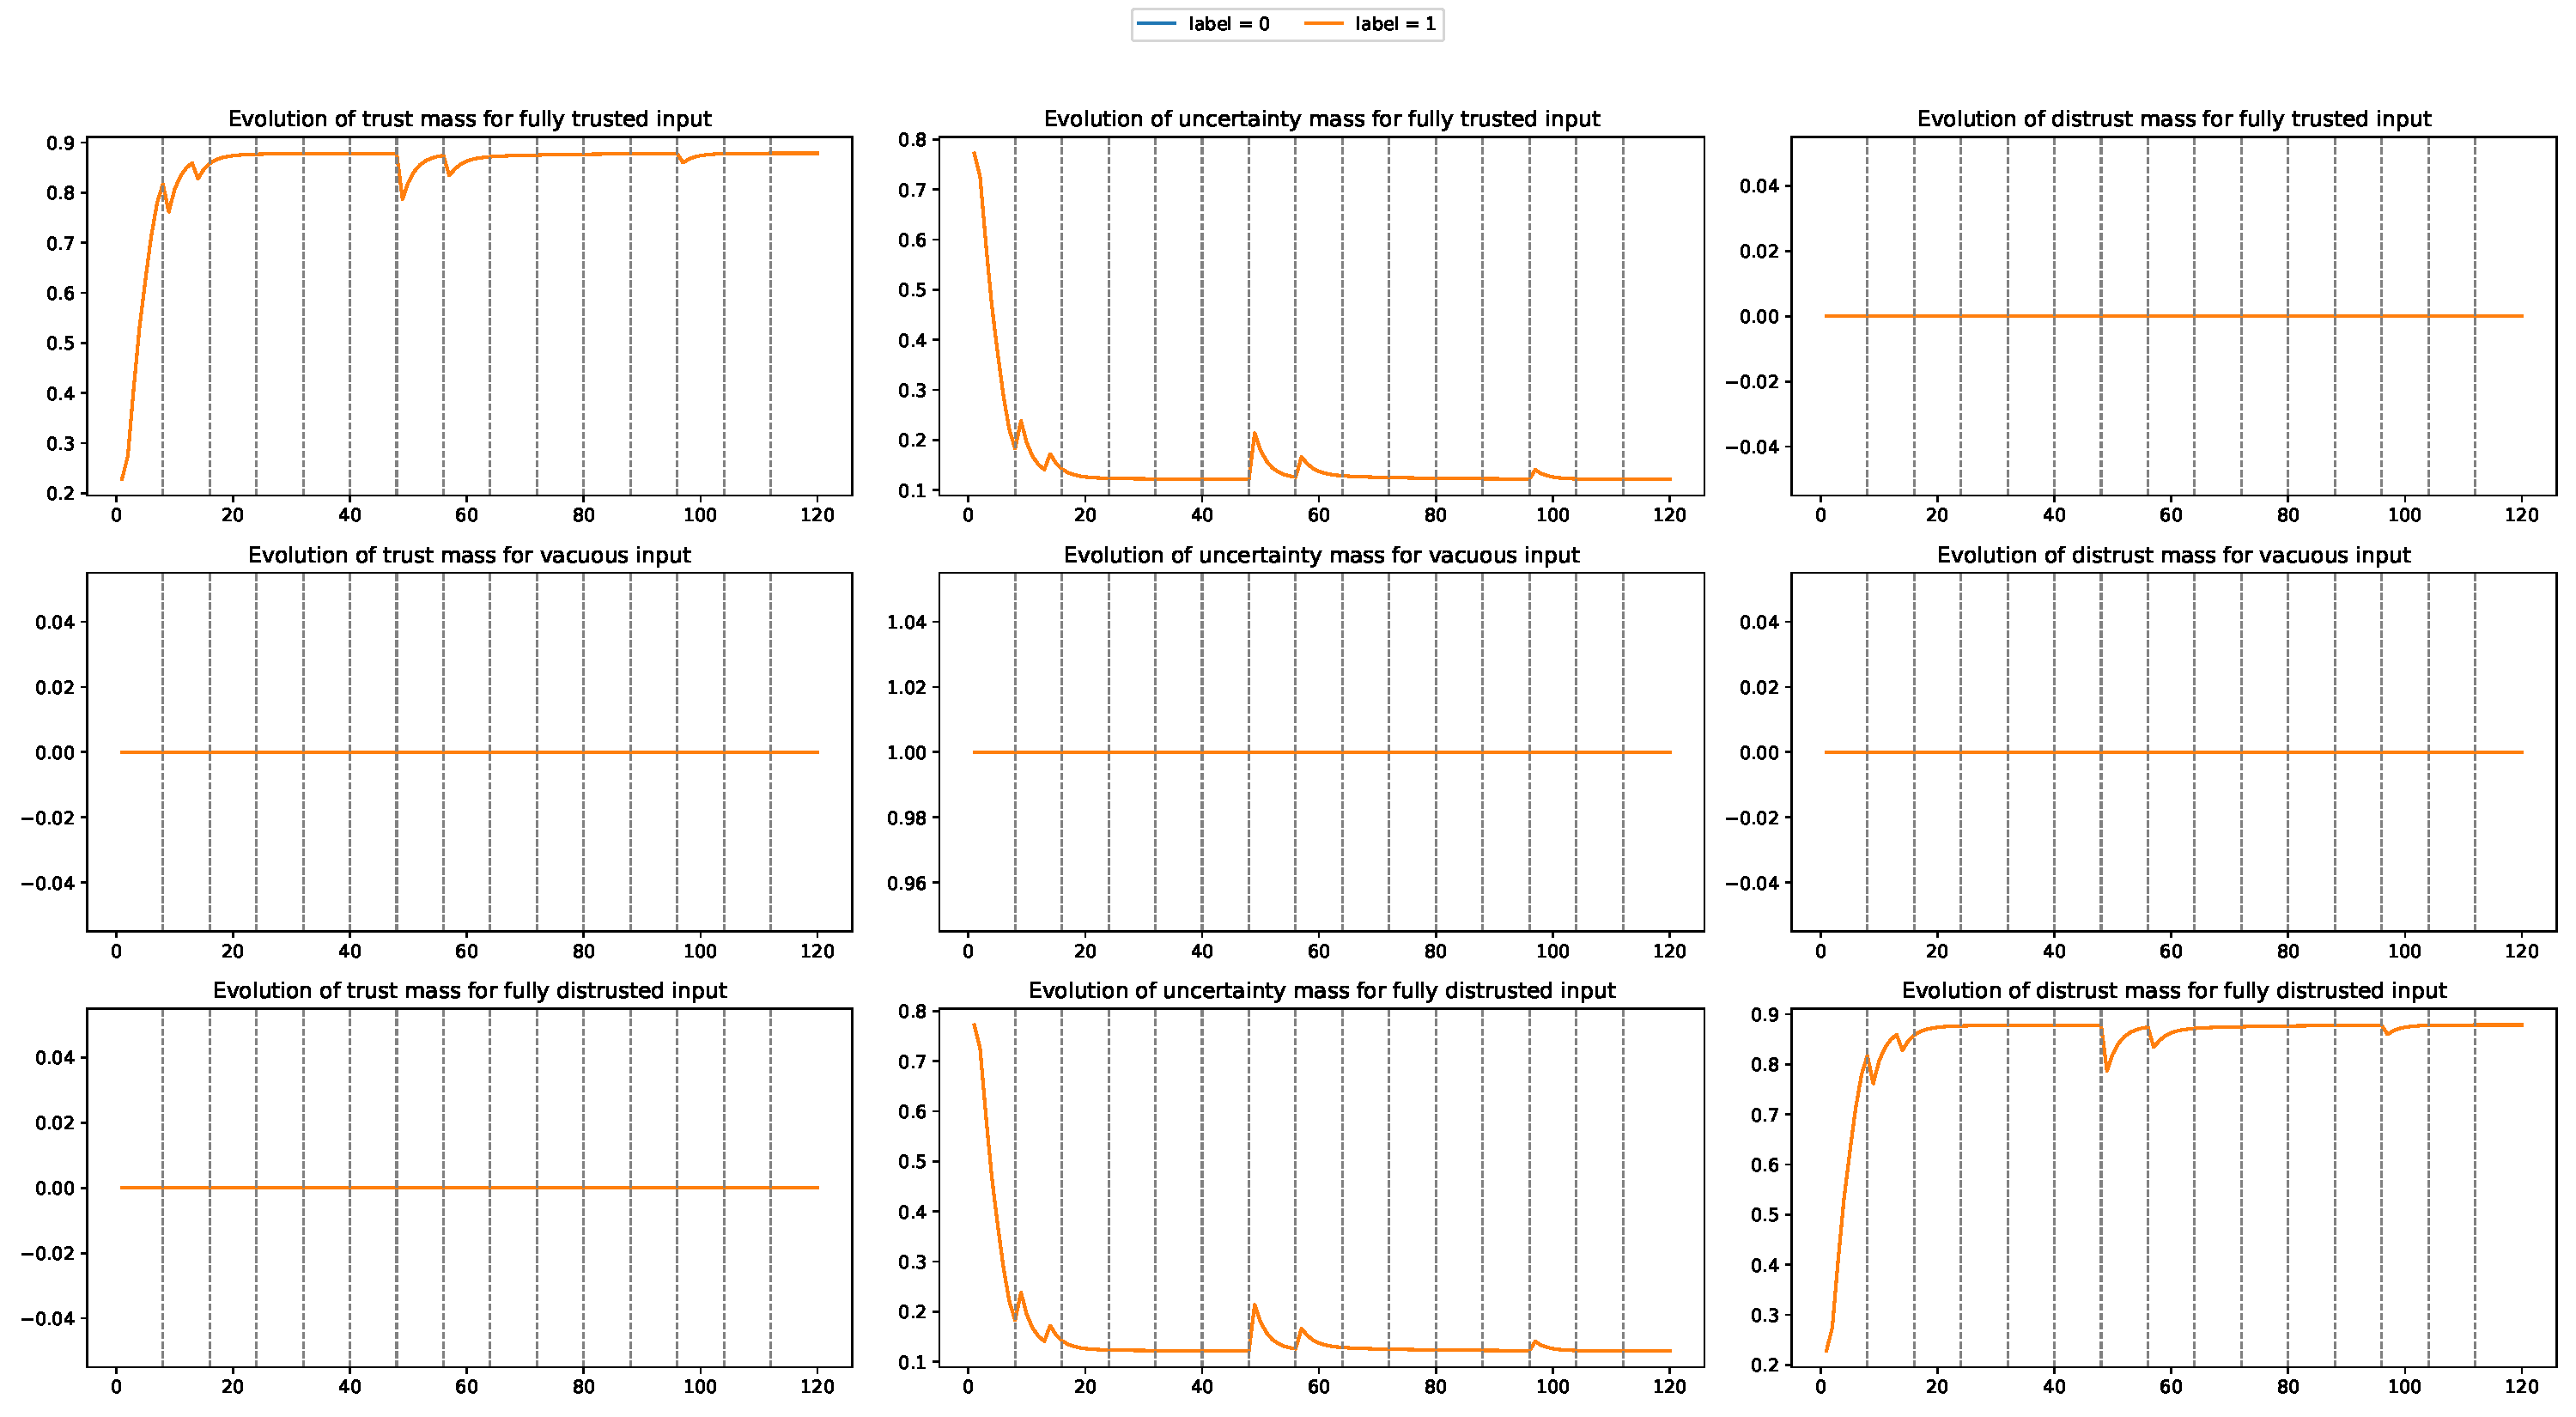
\includegraphics[width=\textwidth]{plots_v2/Cancer/eps=0.1/plot_ptas-t-t.pdf}
  \caption{Features trusted and labels trusted}
\end{figure}

\subsection{Accuracy Evolution for the Cancer Model (\cref{exp:1})}\label{sec:resmnistaccapp}
\begin{figure}[H]
\centering
\begin{subfigure}[b]{0.32\textwidth}
  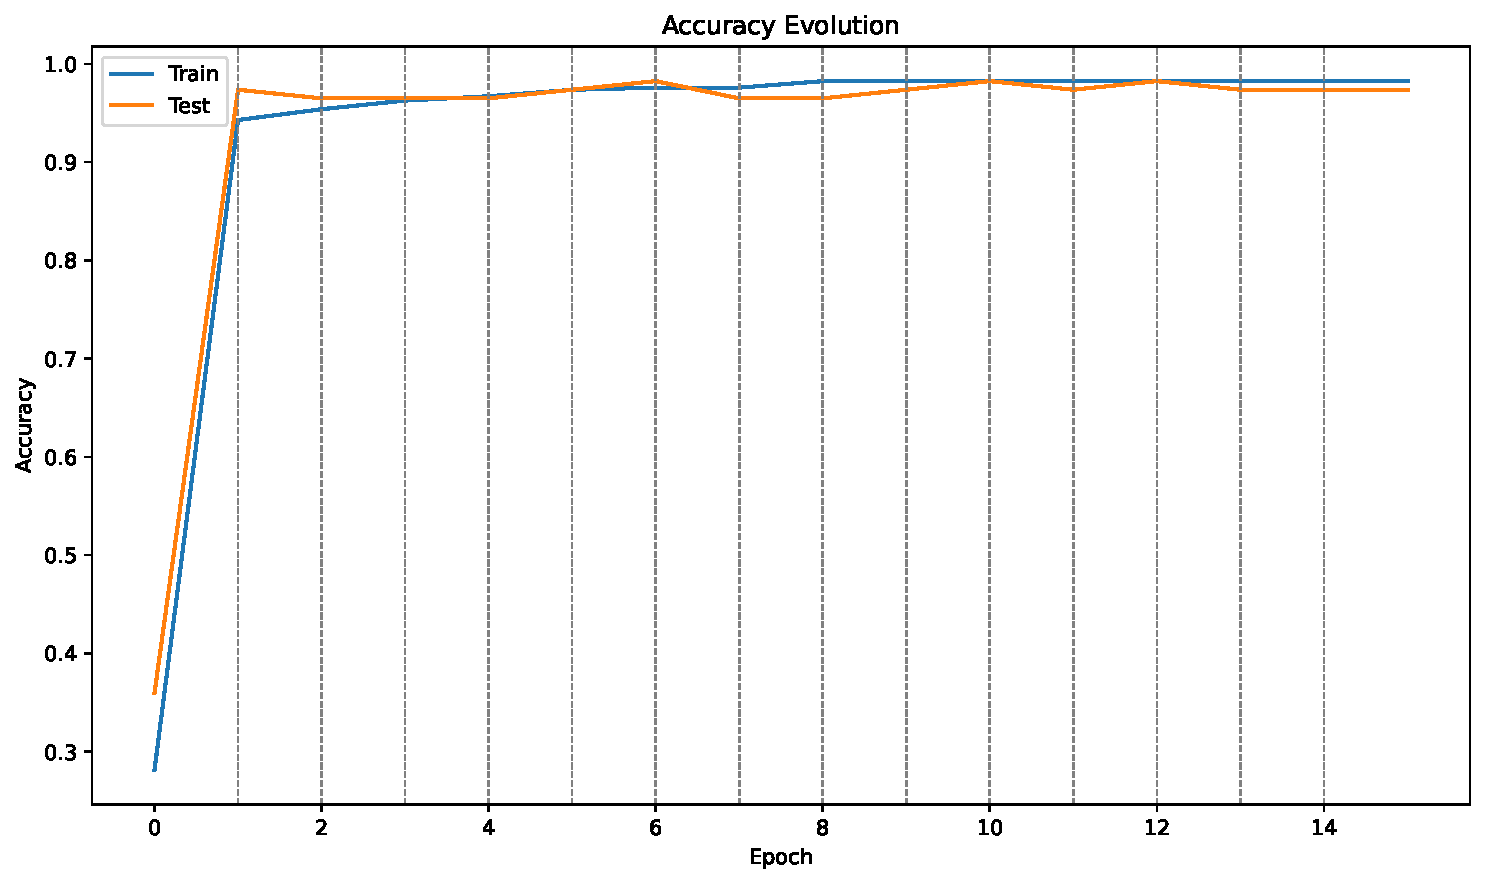
\includegraphics[width=\textwidth]{plots_v2/Cancer/eps=0.1/accuracy_evolution-t-t.pdf}
  \caption{Clean Features and Labels}
\end{subfigure}
\begin{subfigure}[b]{0.32\textwidth}
  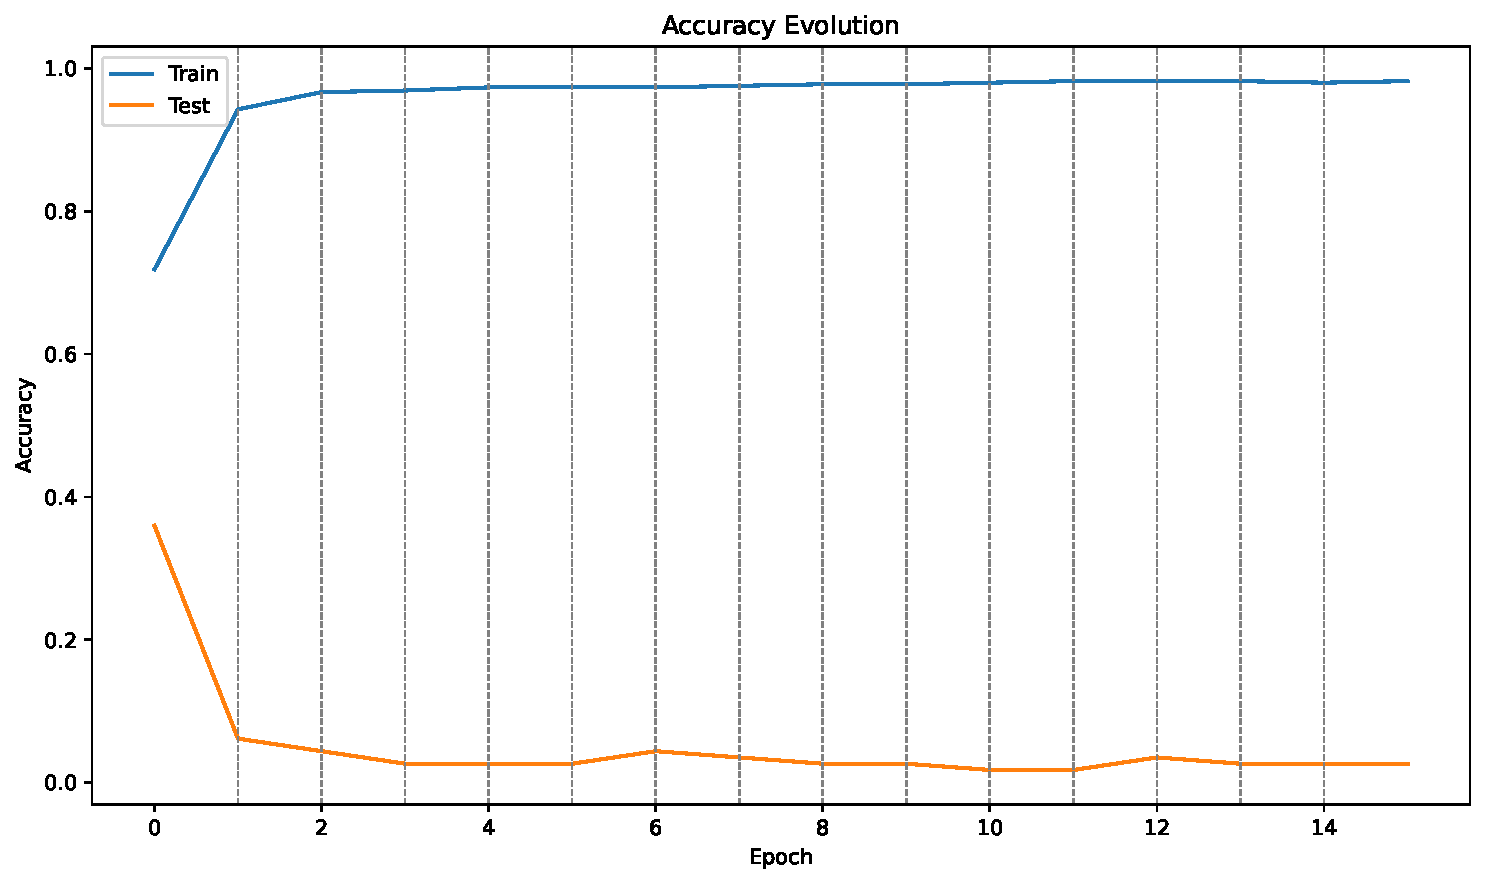
\includegraphics[width=\textwidth]{plots_v2/Cancer/eps=0.1/accuracy_evolution-t-d.pdf}
  \caption{Clean Features and Corrupted Labels}
\end{subfigure}
\begin{subfigure}[b]{0.32\textwidth}
  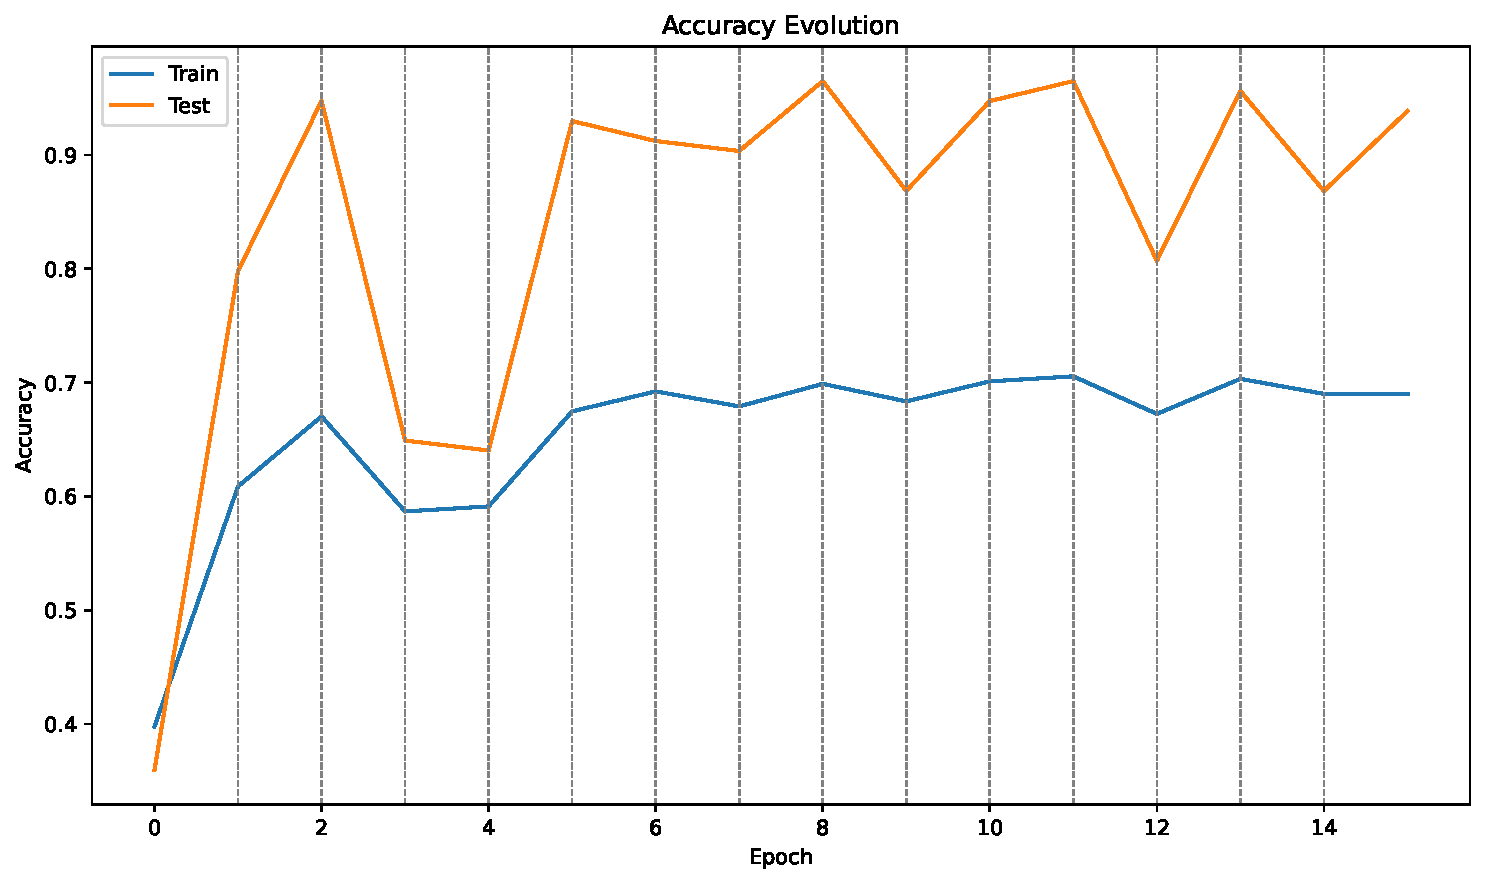
\includegraphics[width=\textwidth]{plots_v2/Cancer/eps=0.1/accuracy_evolution-t-v.pdf}
  \caption{Clean Features and Noisy Labels}
\end{subfigure}
\begin{subfigure}[b]{0.32\textwidth}
  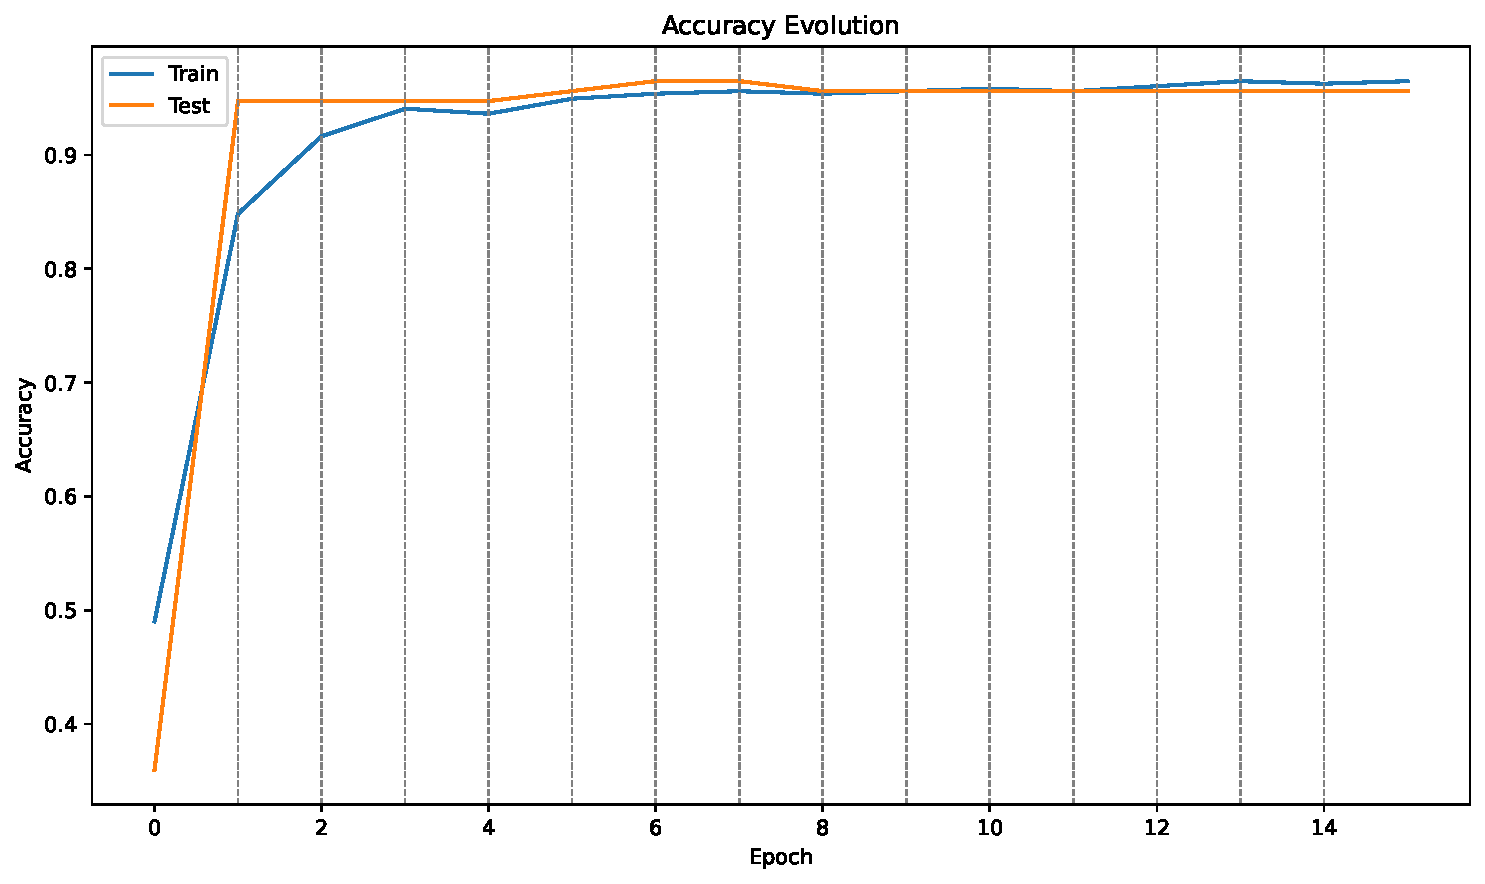
\includegraphics[width=\textwidth]{plots_v2/Cancer/eps=0.1/accuracy_evolution-v-t.pdf}
  \caption{Noisy Features and Clean Labels}
\end{subfigure}
\begin{subfigure}[b]{0.32\textwidth}
  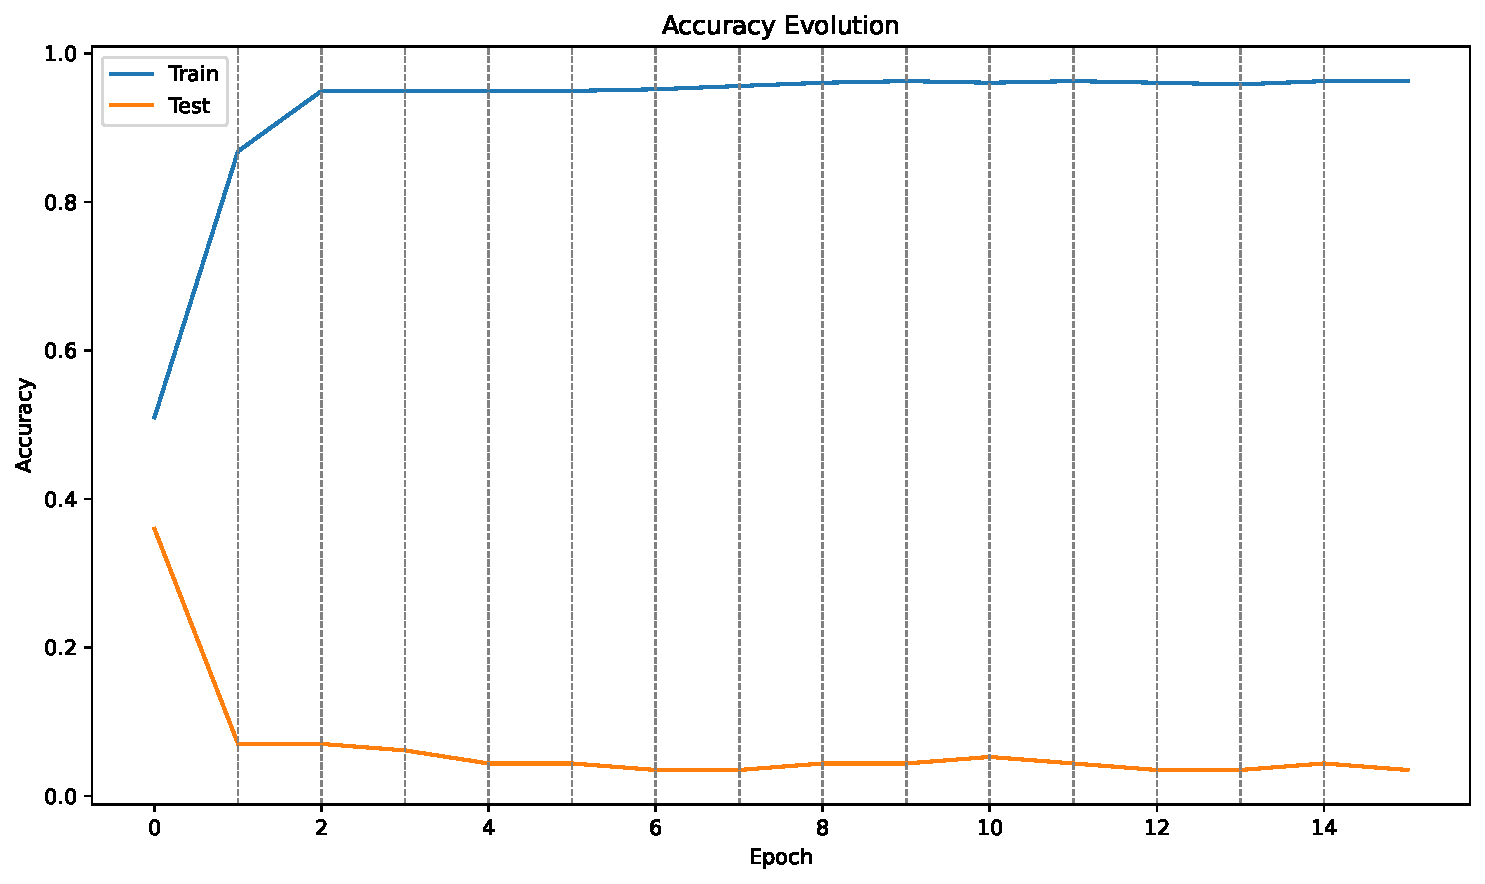
\includegraphics[width=\textwidth]{plots_v2/Cancer/eps=0.1/accuracy_evolution-v-d.pdf}
  \caption{Noisy Features and Corrupted Labels}
\end{subfigure}
\begin{subfigure}[b]{0.32\textwidth}
  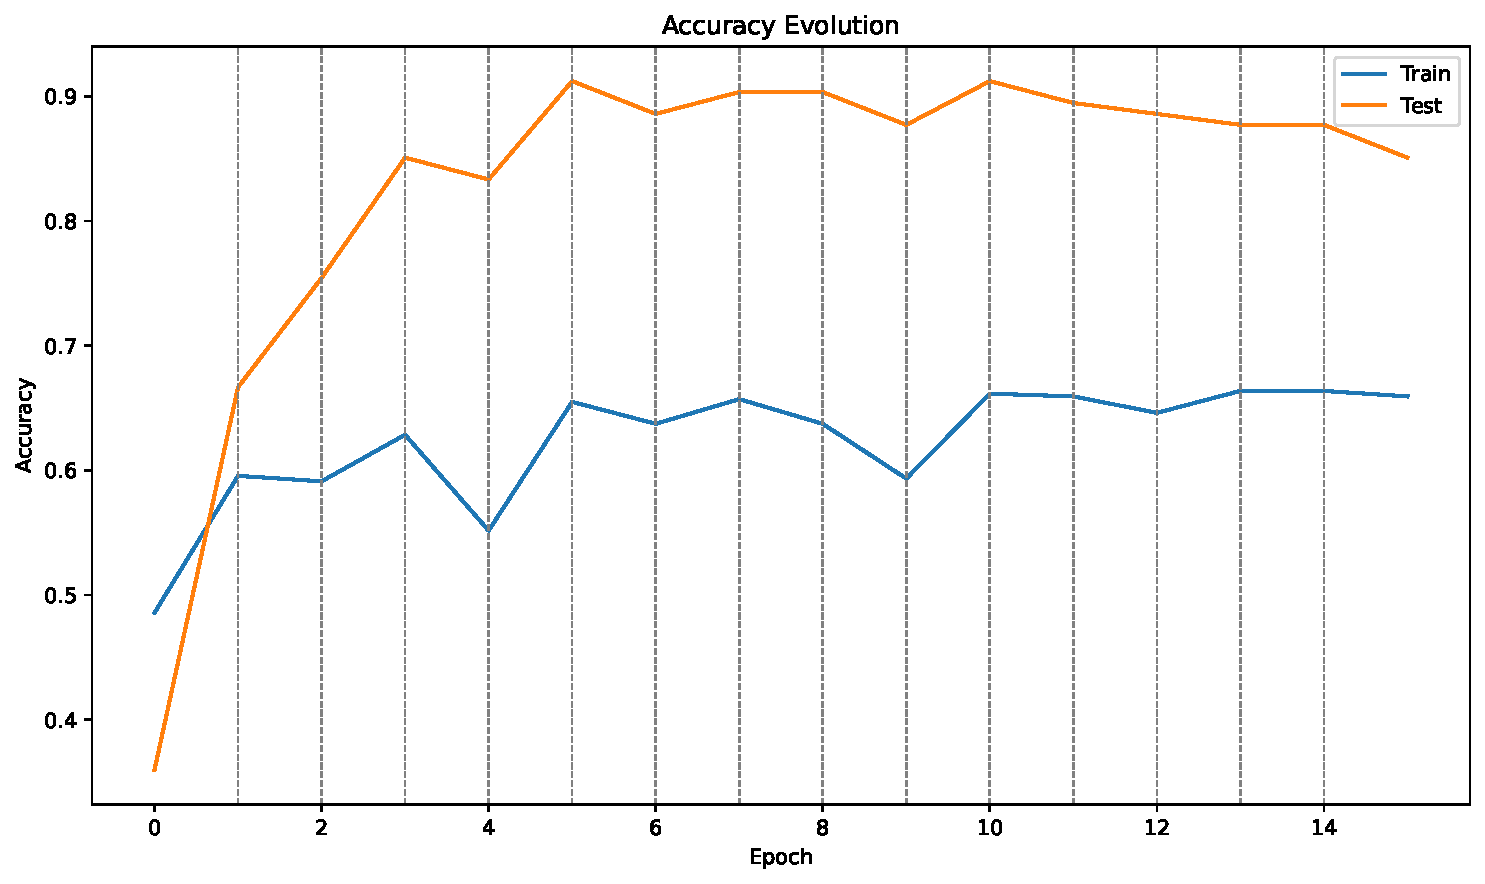
\includegraphics[width=\textwidth]{plots_v2/Cancer/eps=0.1/accuracy_evolution-v-v.pdf}
  \caption{Noisy Features and Noisy Labels}
\end{subfigure}
\begin{subfigure}[b]{0.32\textwidth}
  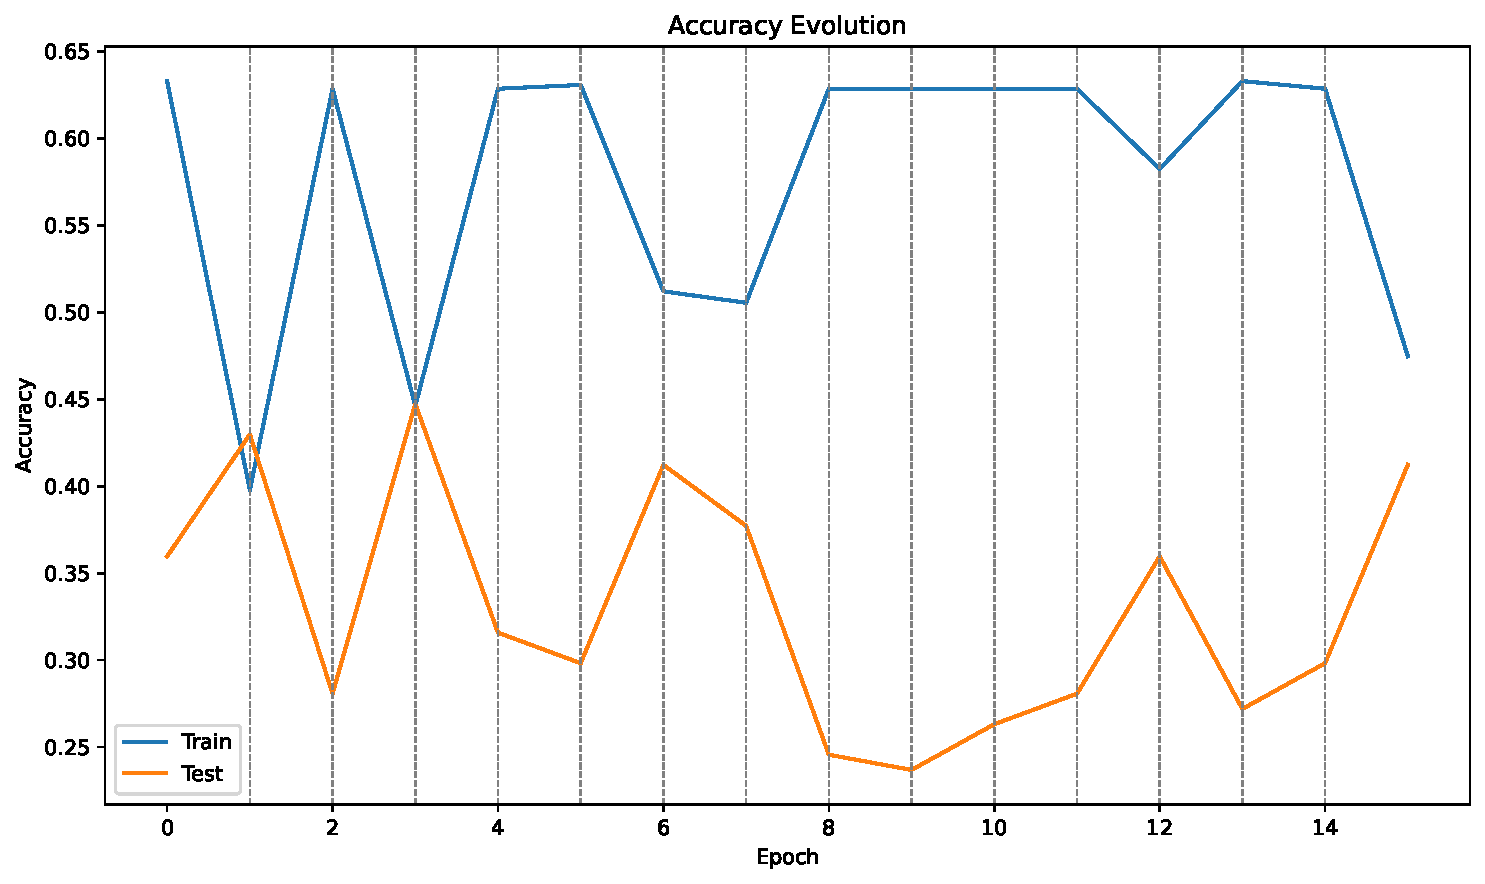
\includegraphics[width=\textwidth]{plots_v2/Cancer/eps=0.1/accuracy_evolution-d-t.pdf}
  \caption{Corrupted Features and Clean Labels}
\end{subfigure}
\begin{subfigure}[b]{0.32\textwidth}
  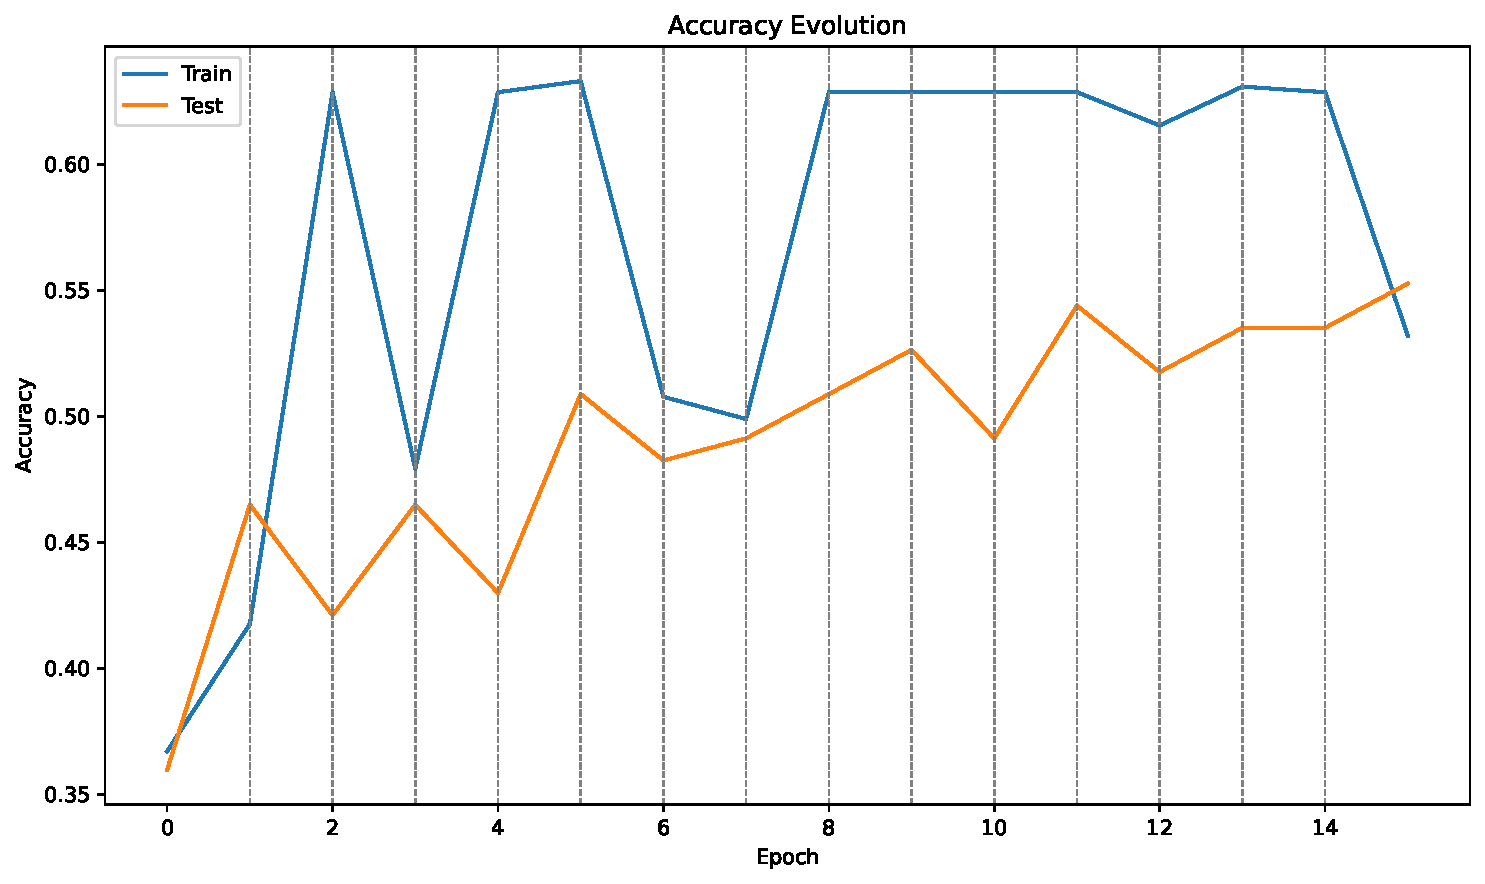
\includegraphics[width=\textwidth]{plots_v2/Cancer/eps=0.1/accuracy_evolution-d-d.pdf}
  \caption{Corrupted Features and Corrupted Labels}
\end{subfigure}
\begin{subfigure}[b]{0.32\textwidth}
  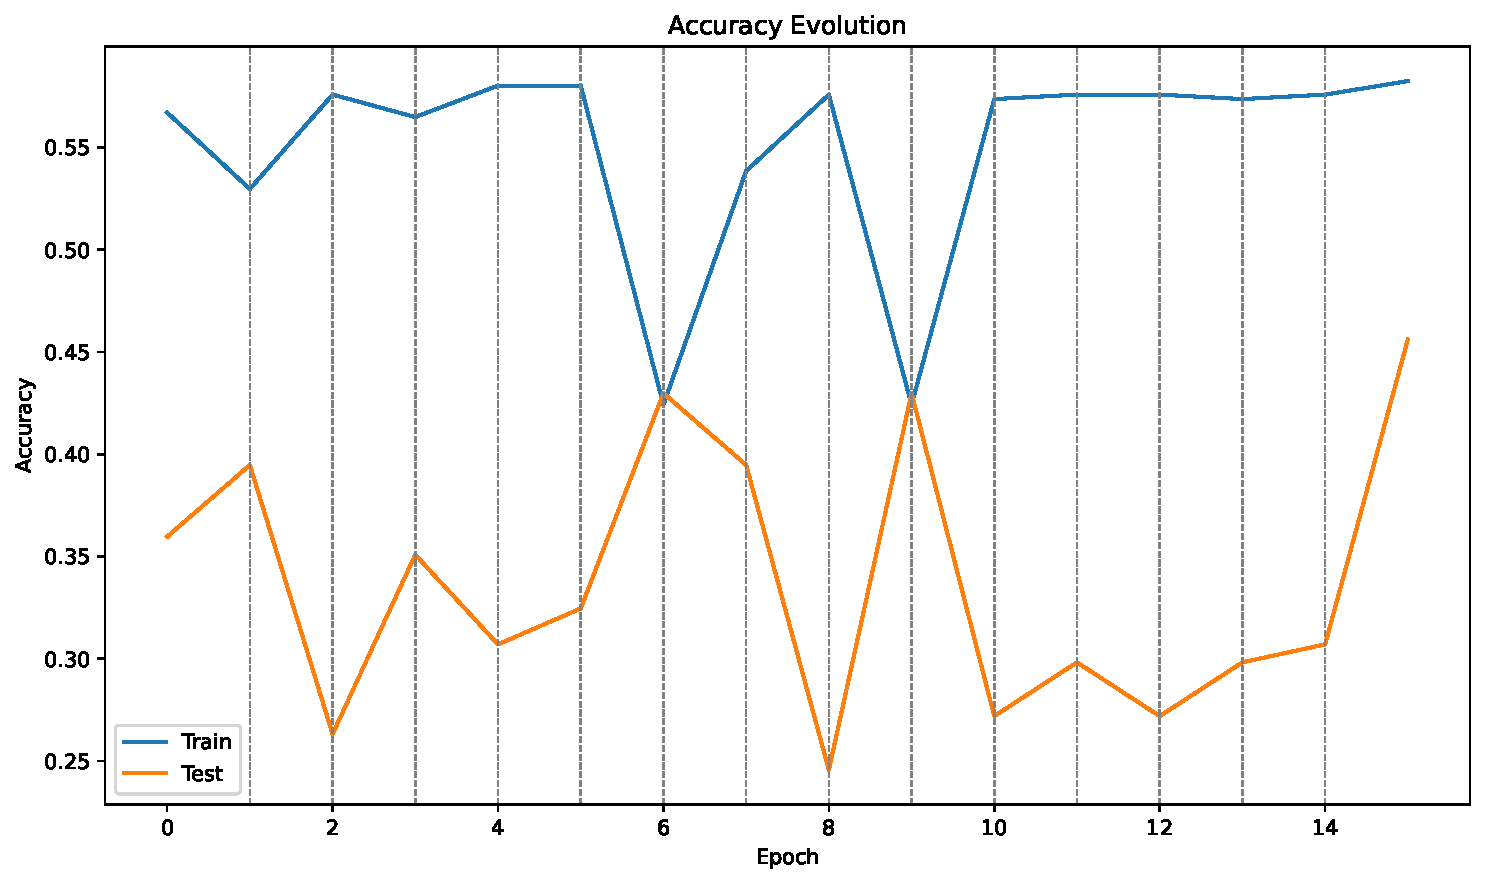
\includegraphics[width=\textwidth]{plots_v2/Cancer/eps=0.1/accuracy_evolution-d-v.pdf}
  \caption{Corrupted Features and Noisy Labels}
\end{subfigure}
\caption{Accuracy evolution of the Cancer model under different combinations of clean, corrupted, and noisy features and labels.}
\label{fig:Acccancer}
\end{figure}
% \begin{figure}[H]
%     \centering
%     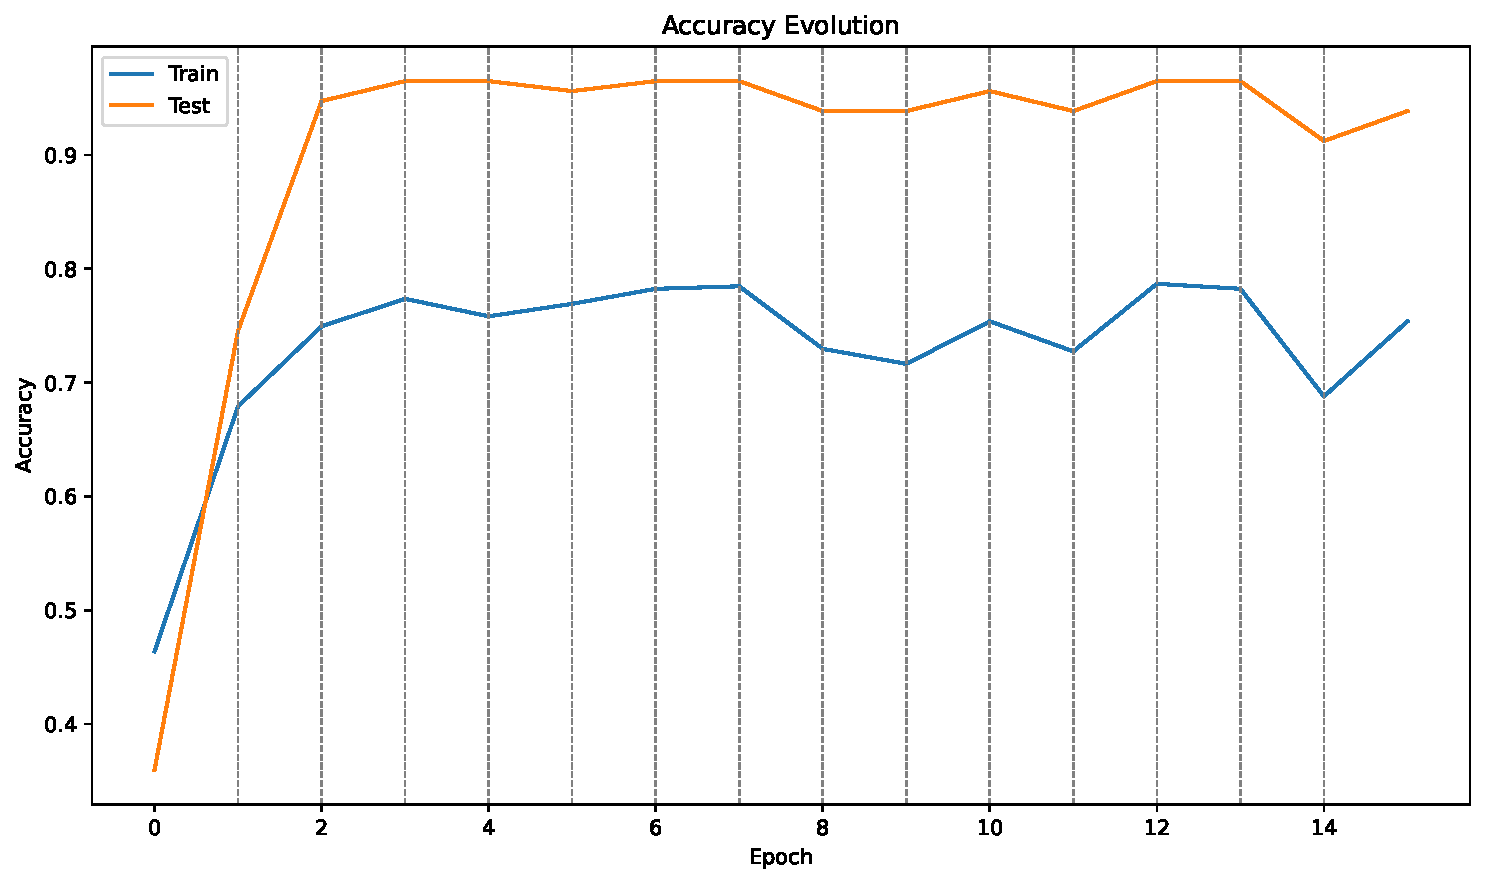
\includegraphics[width=0.8\linewidth]{good_plots/accuracy/Cancer/0.15-0.25/Cancer-noise-noise.pdf}
%     \caption{Accuracy evolution of the Cancer model when reducing the noise for noised features and labels.}
%     \label{fig:AcccancerInt}
% \end{figure}

\subsection{MNIST with Vacuous Trust Assessment (\cref{exp:2})}\label{sec:resmnist}
\begin{figure}[H]
  \centering
  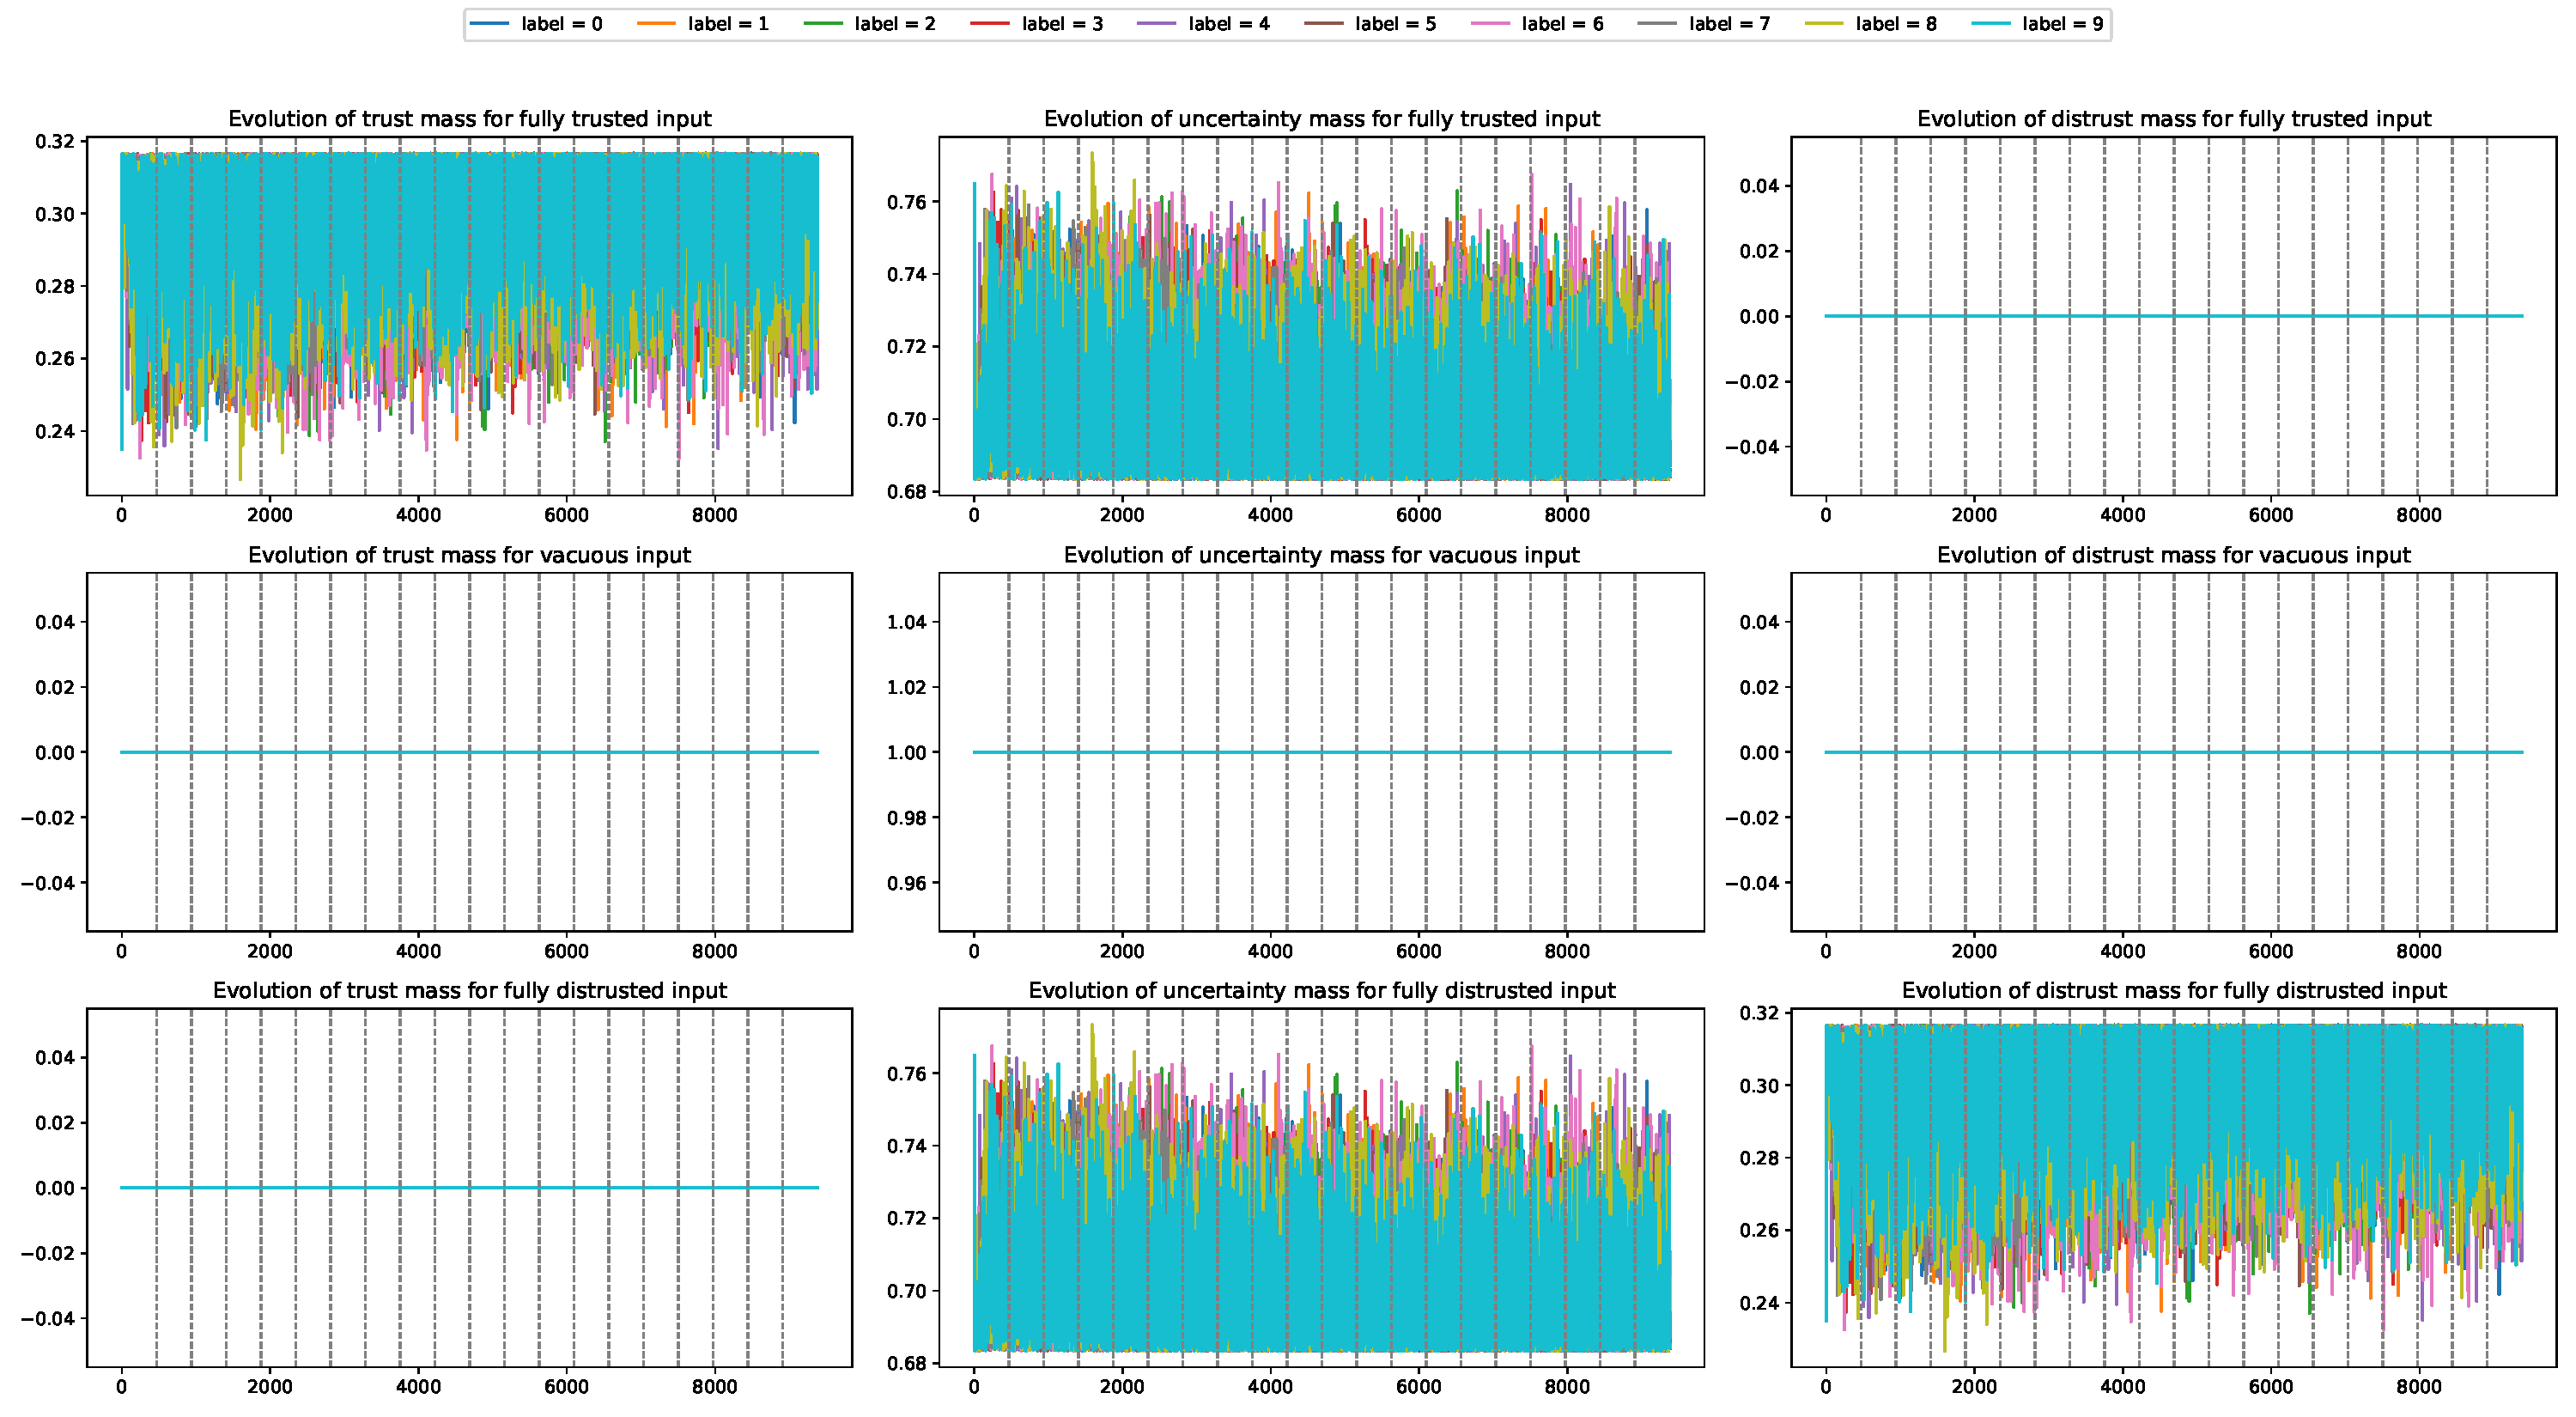
\includegraphics[width=\textwidth]{plots_v2/MNIST/architecture/plot_ptas-16-v-v.pdf}
  \caption{16 Hidden neurons}
\end{figure}
\begin{figure}[H]
  \centering
  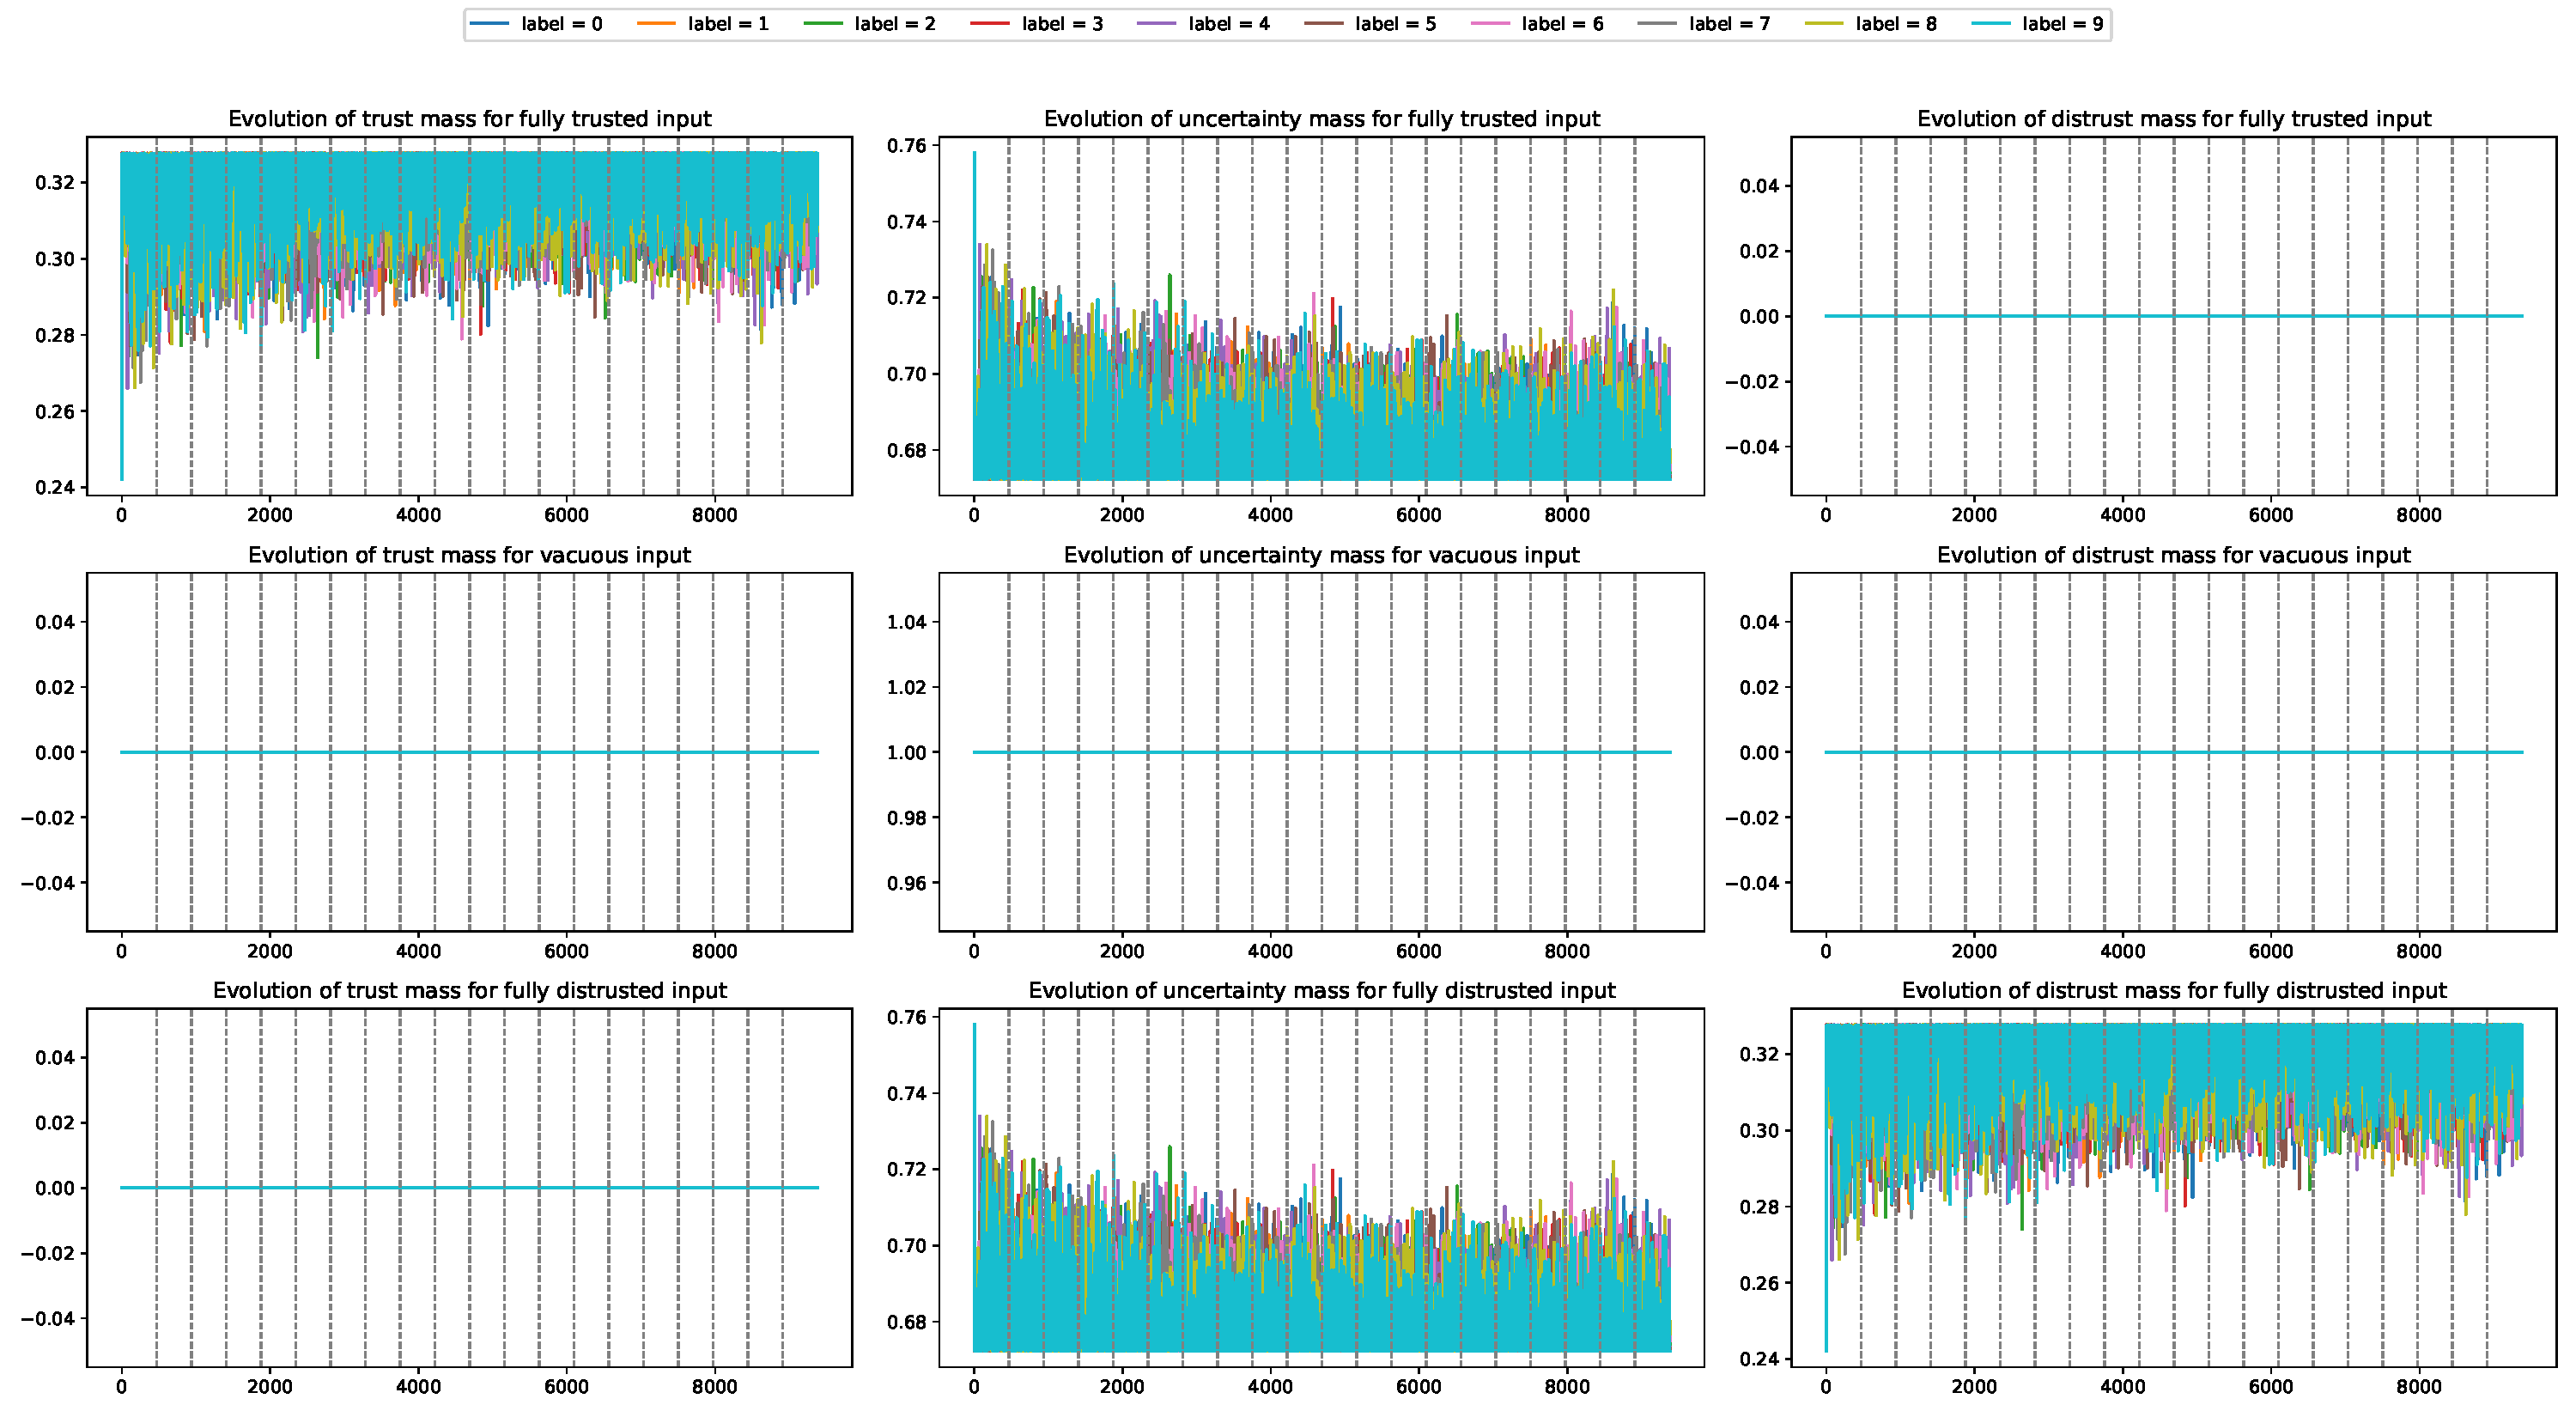
\includegraphics[width=\textwidth]{plots_v2/MNIST/architecture/plot_ptas-32-v-v.pdf}
  \caption{32 Hidden neurons}
\end{figure}
\begin{figure}[H]
  \centering
  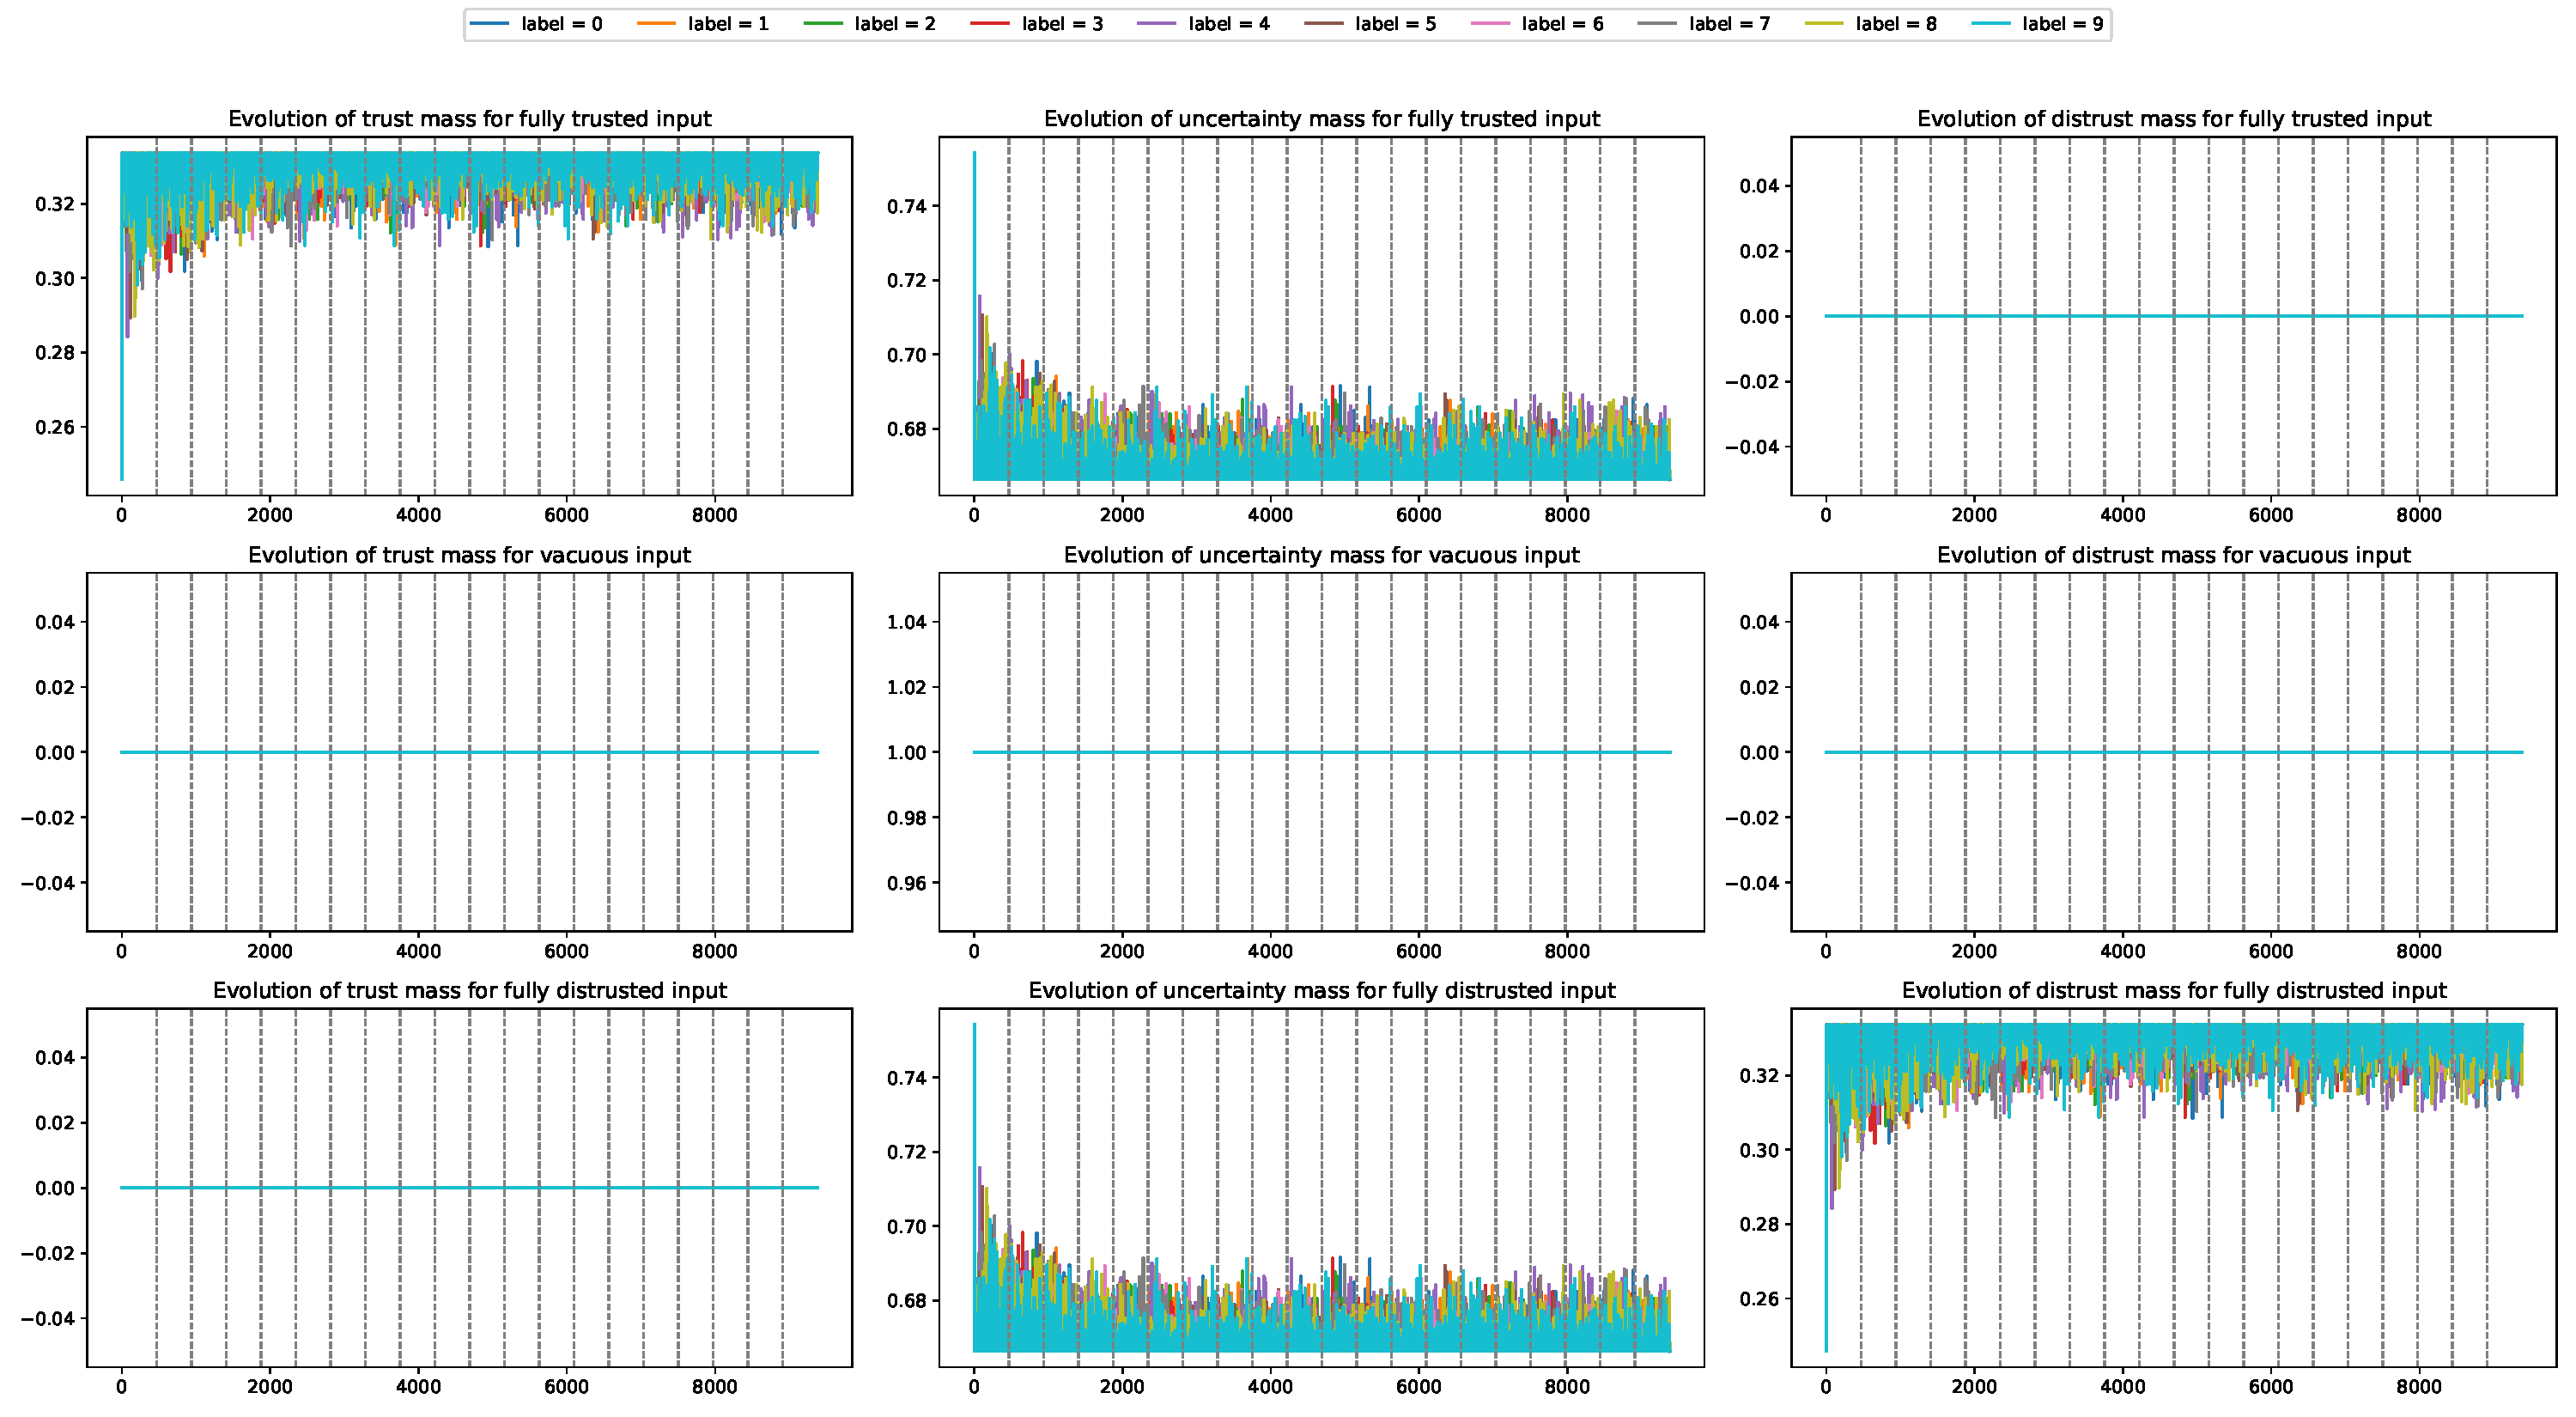
\includegraphics[width=\textwidth]{plots_v2/MNIST/architecture/plot_ptas-64-v-v.pdf}
  \caption{64 Hidden neurons}
\end{figure}
\begin{figure}[H]
  \centering
  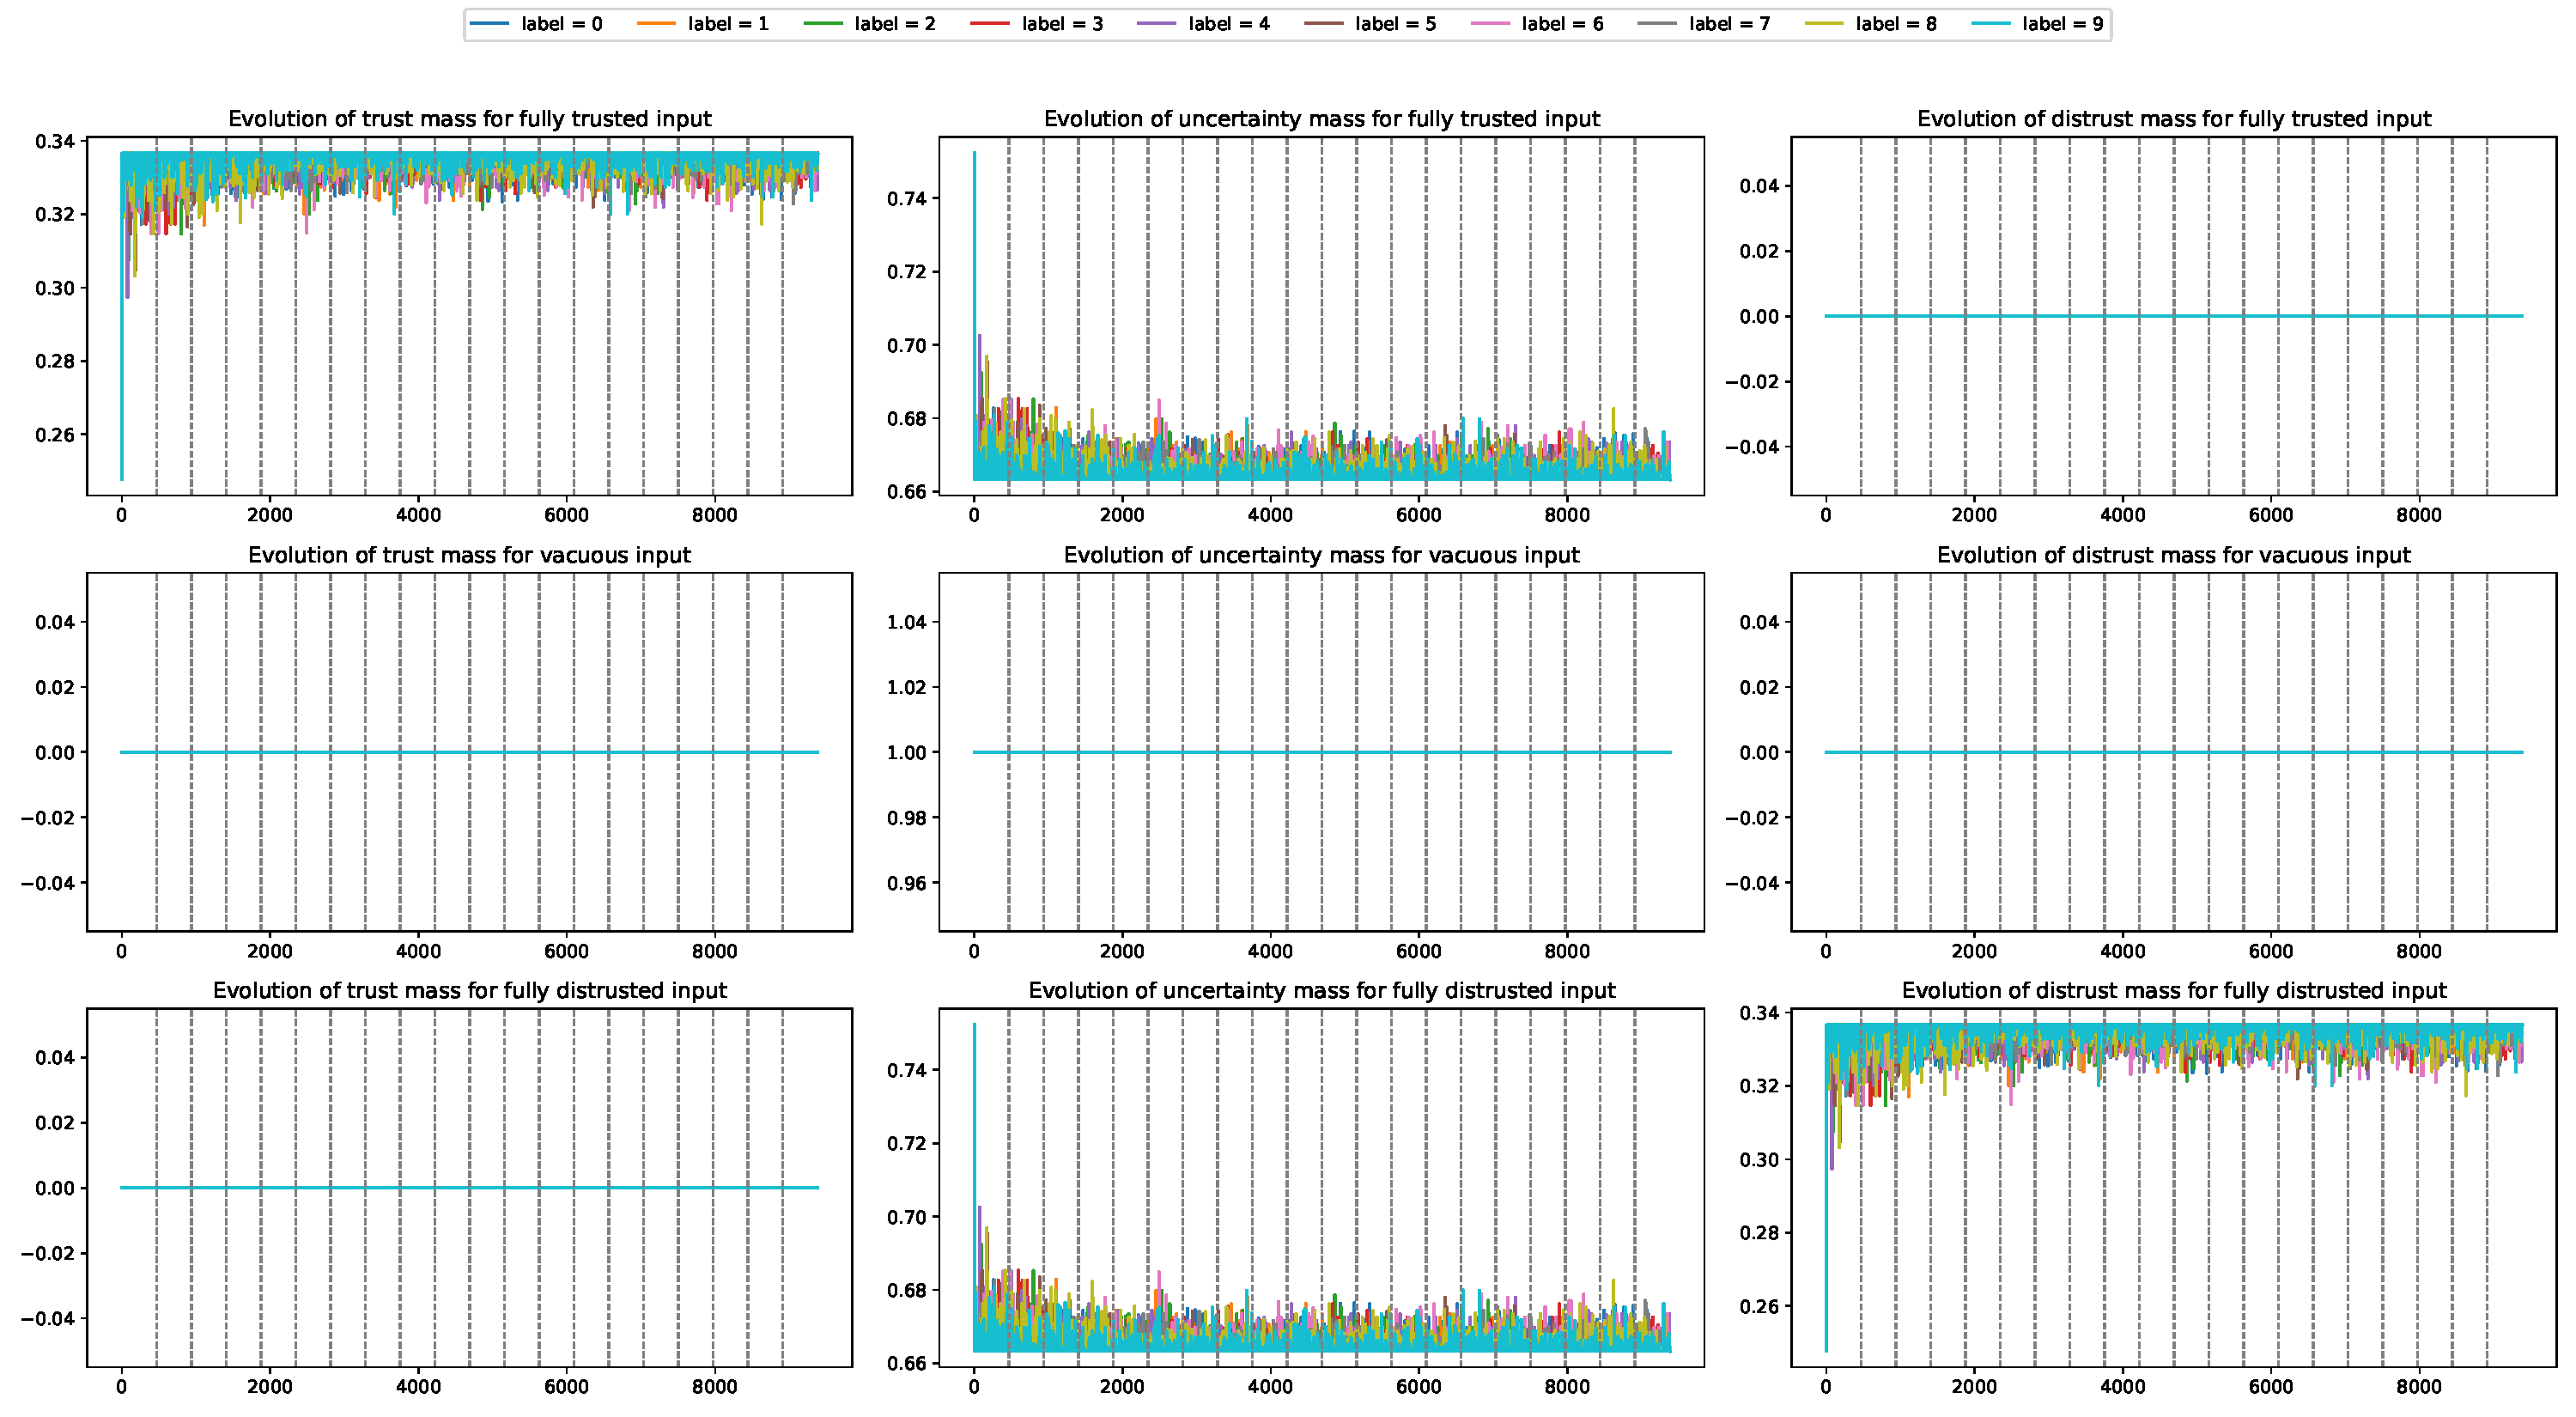
\includegraphics[width=\textwidth]{plots_v2/MNIST/architecture/plot_ptas-128-v-v.pdf}
  \caption{128 Hidden neurons}
\end{figure}
\begin{figure}[H]
  \centering
  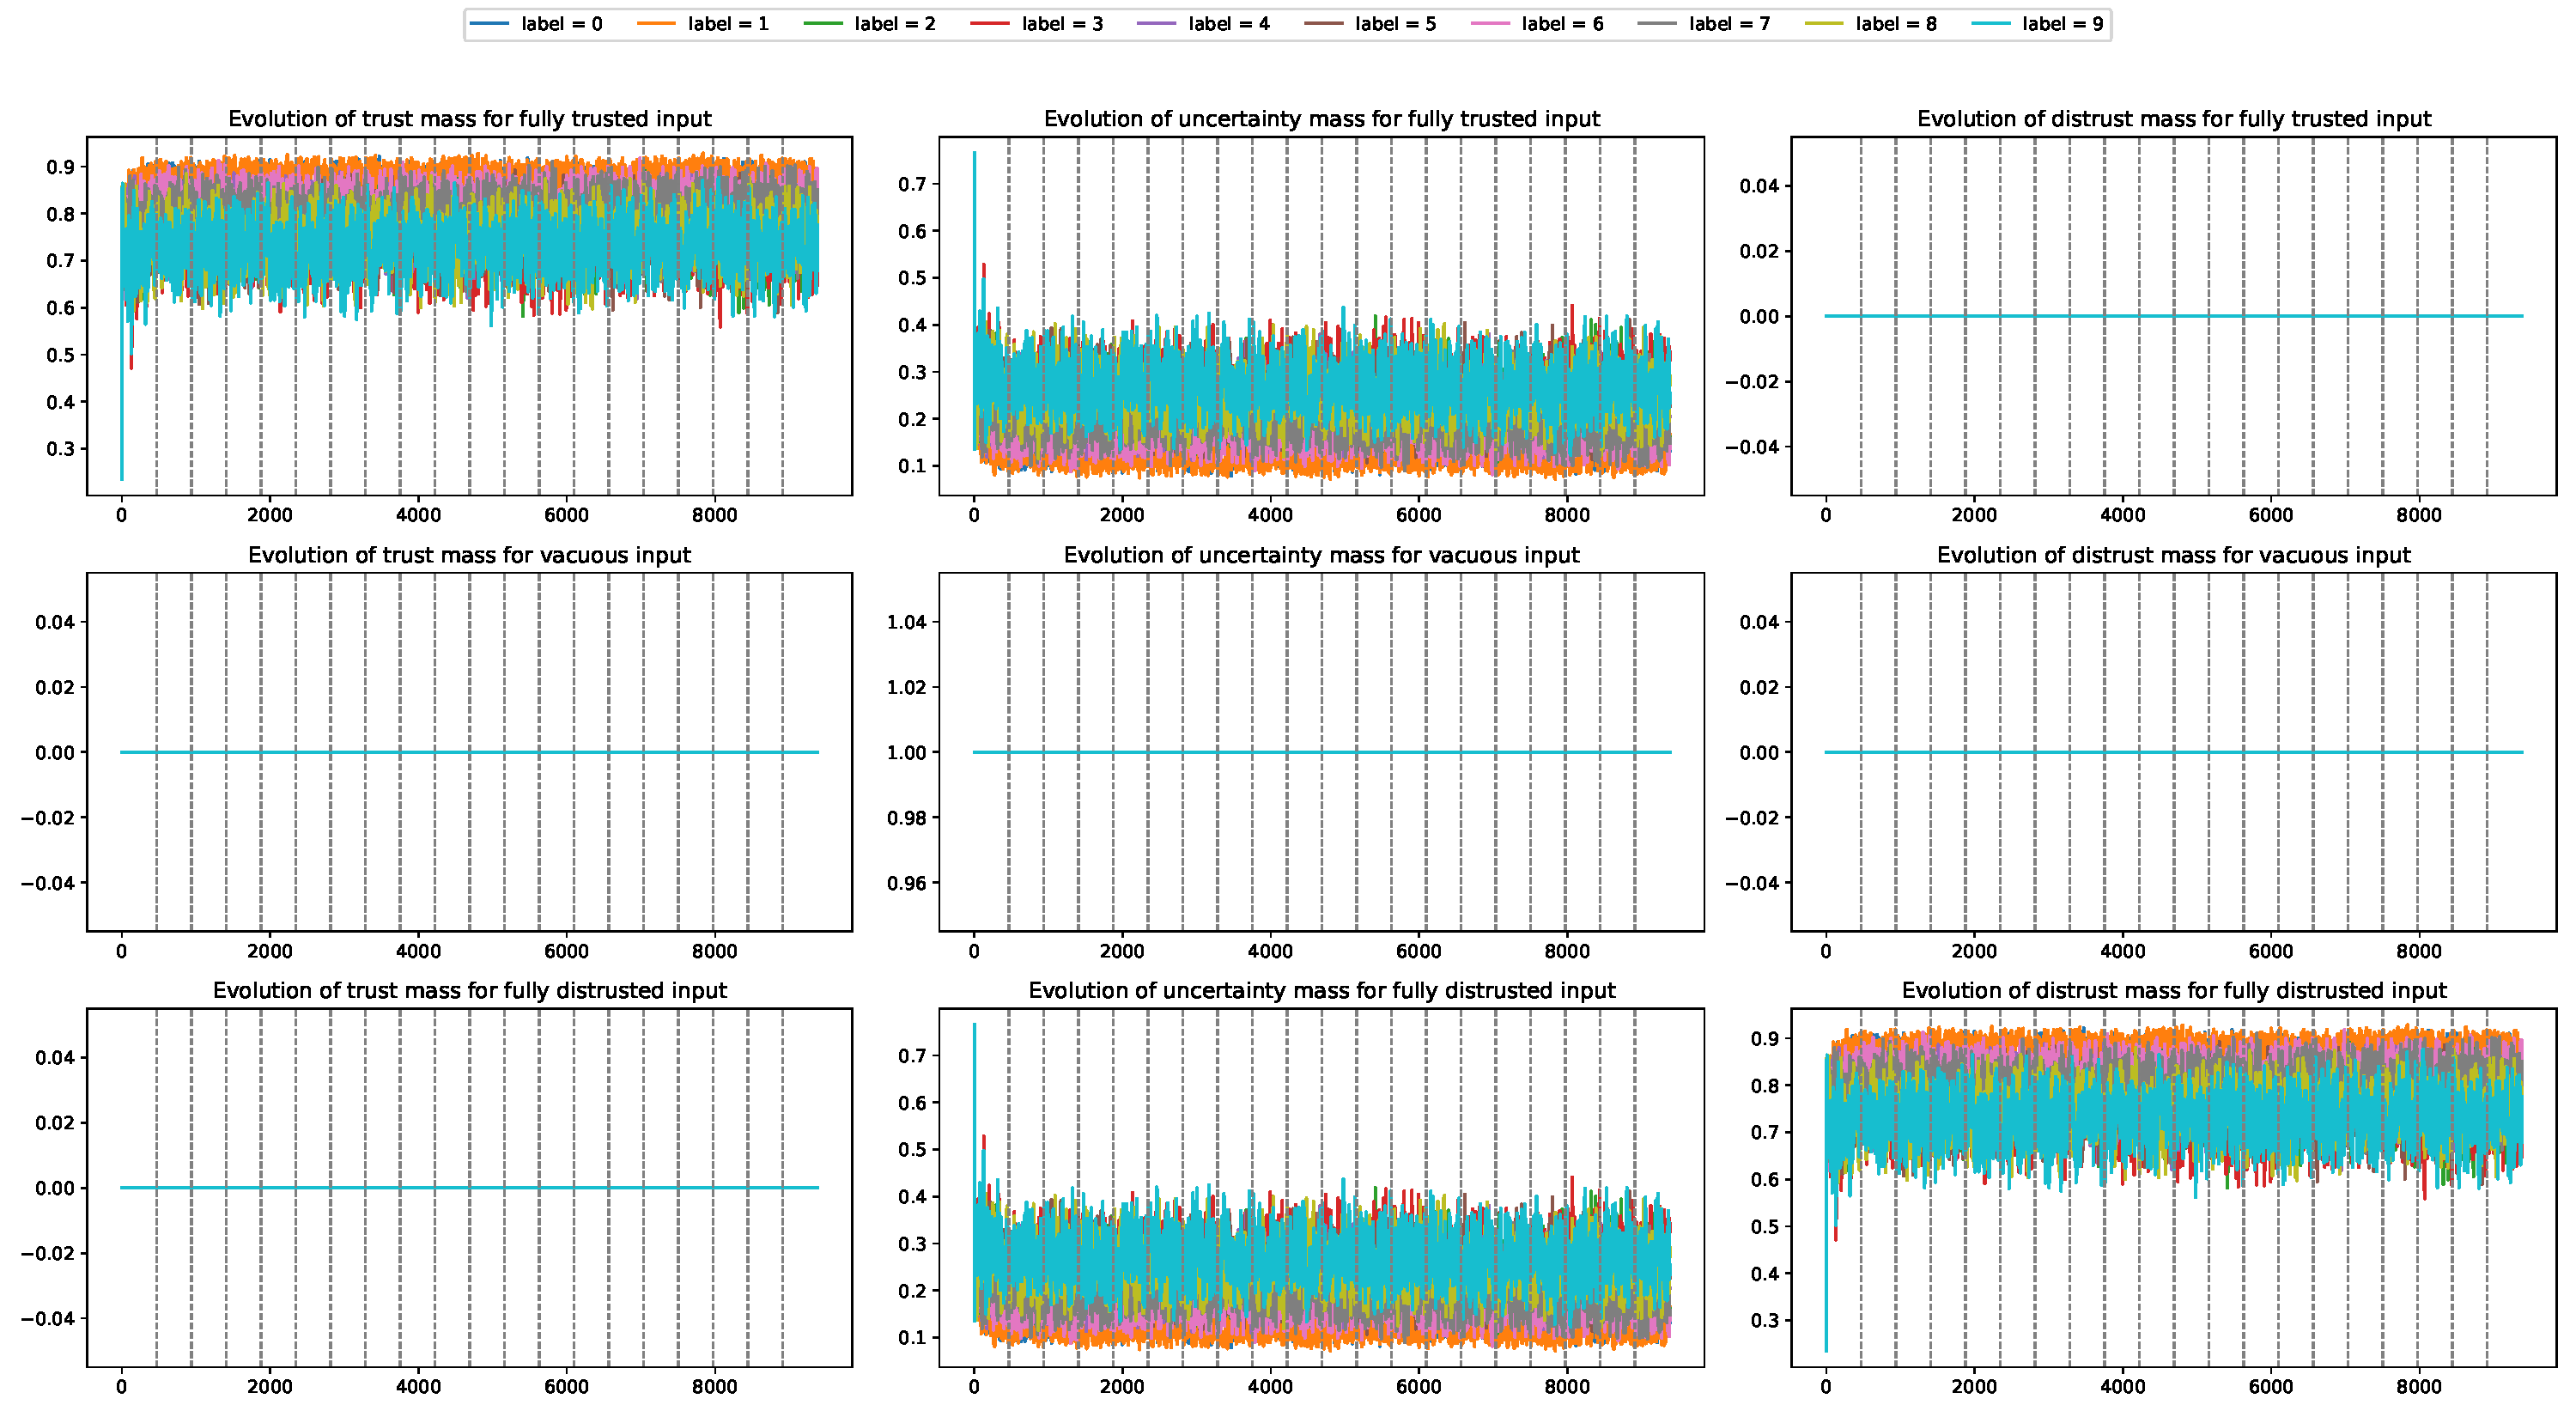
\includegraphics[width=\textwidth]{plots_v2/MNIST/architecture/plot_ptas-16-t-t.pdf}
  \caption{16 Hidden neurons with Fully Trusted Assessment}
\end{figure}

\subsection{MNIST poisoned 128 hidden neurons (\cref{exp:3})}\label{sec:resmnistpois}
\begin{figure}[H]
  \centering
  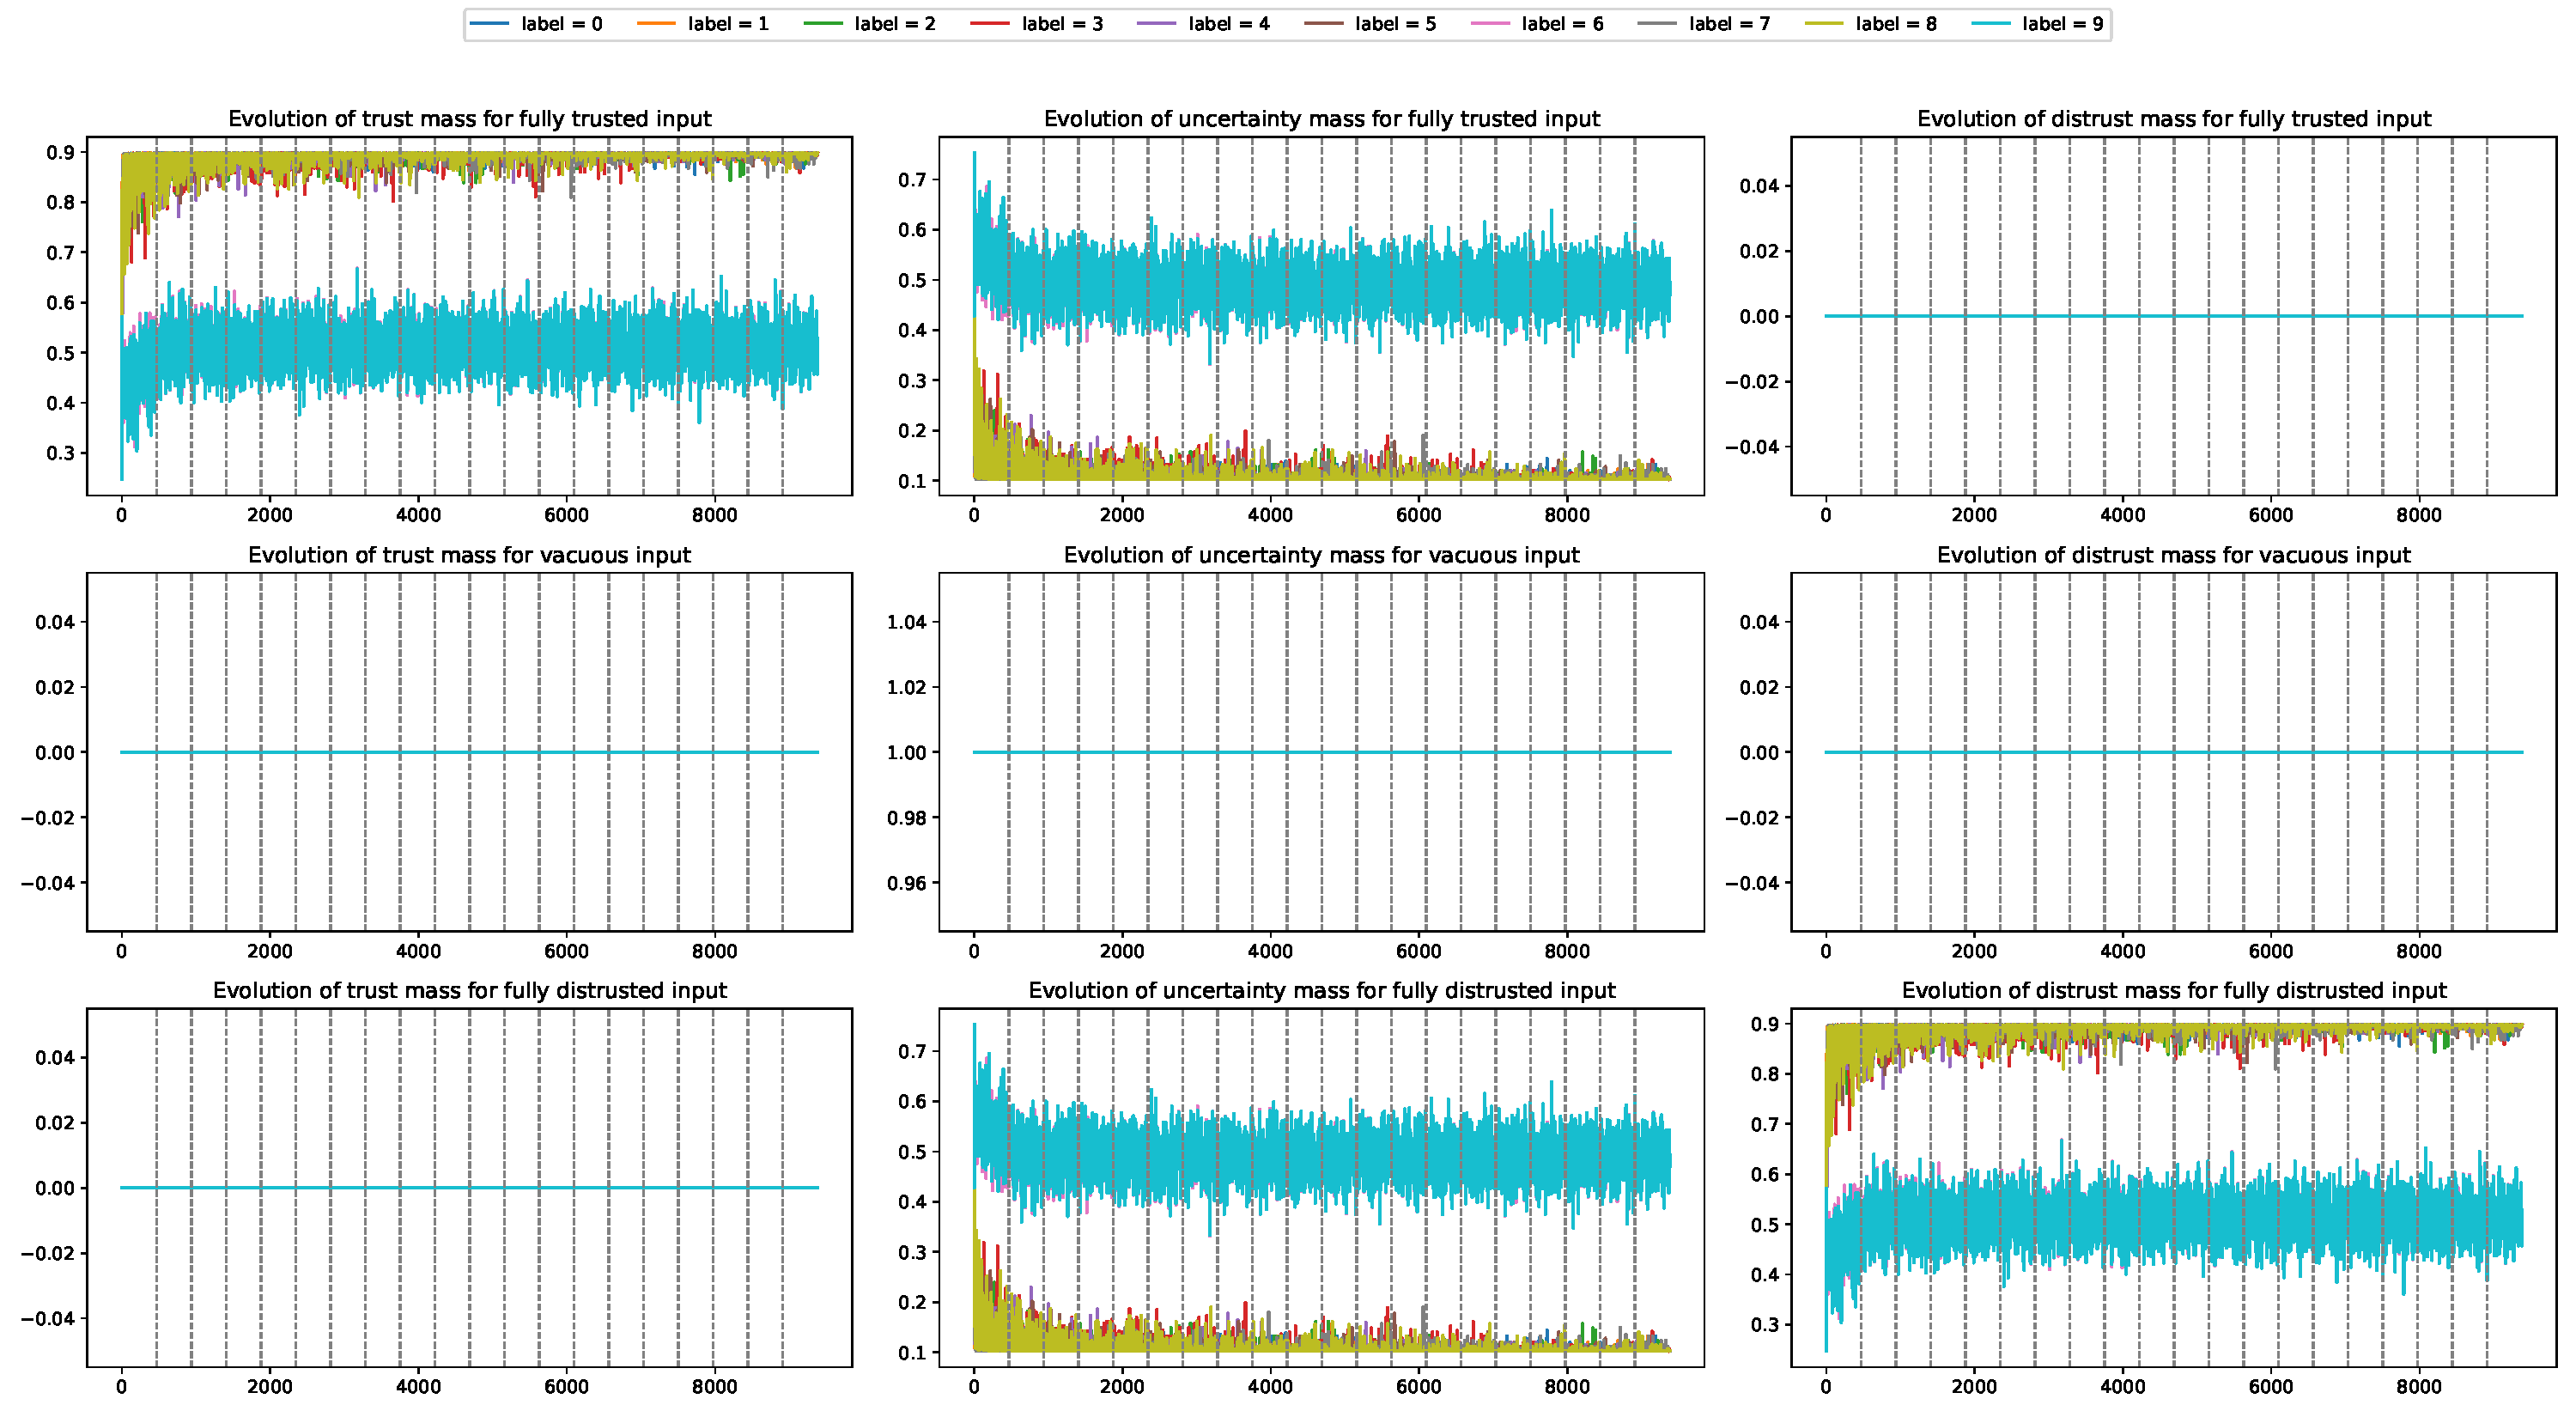
\includegraphics[width=\textwidth]{plots_v2/MNIST/poisoned/plot_ptas-128-t-t-ps1.pdf}
  \caption{1 pixel}
\end{figure}
\begin{figure}[H]
  \centering
  \includegraphics[width=\textwidth]{plots_v2/MNIST/poisoned/plot_ptas-128-t-t-ps4.pdf}
  \caption{4×4 pixels}
\end{figure}
\begin{figure}[H]
  \centering
  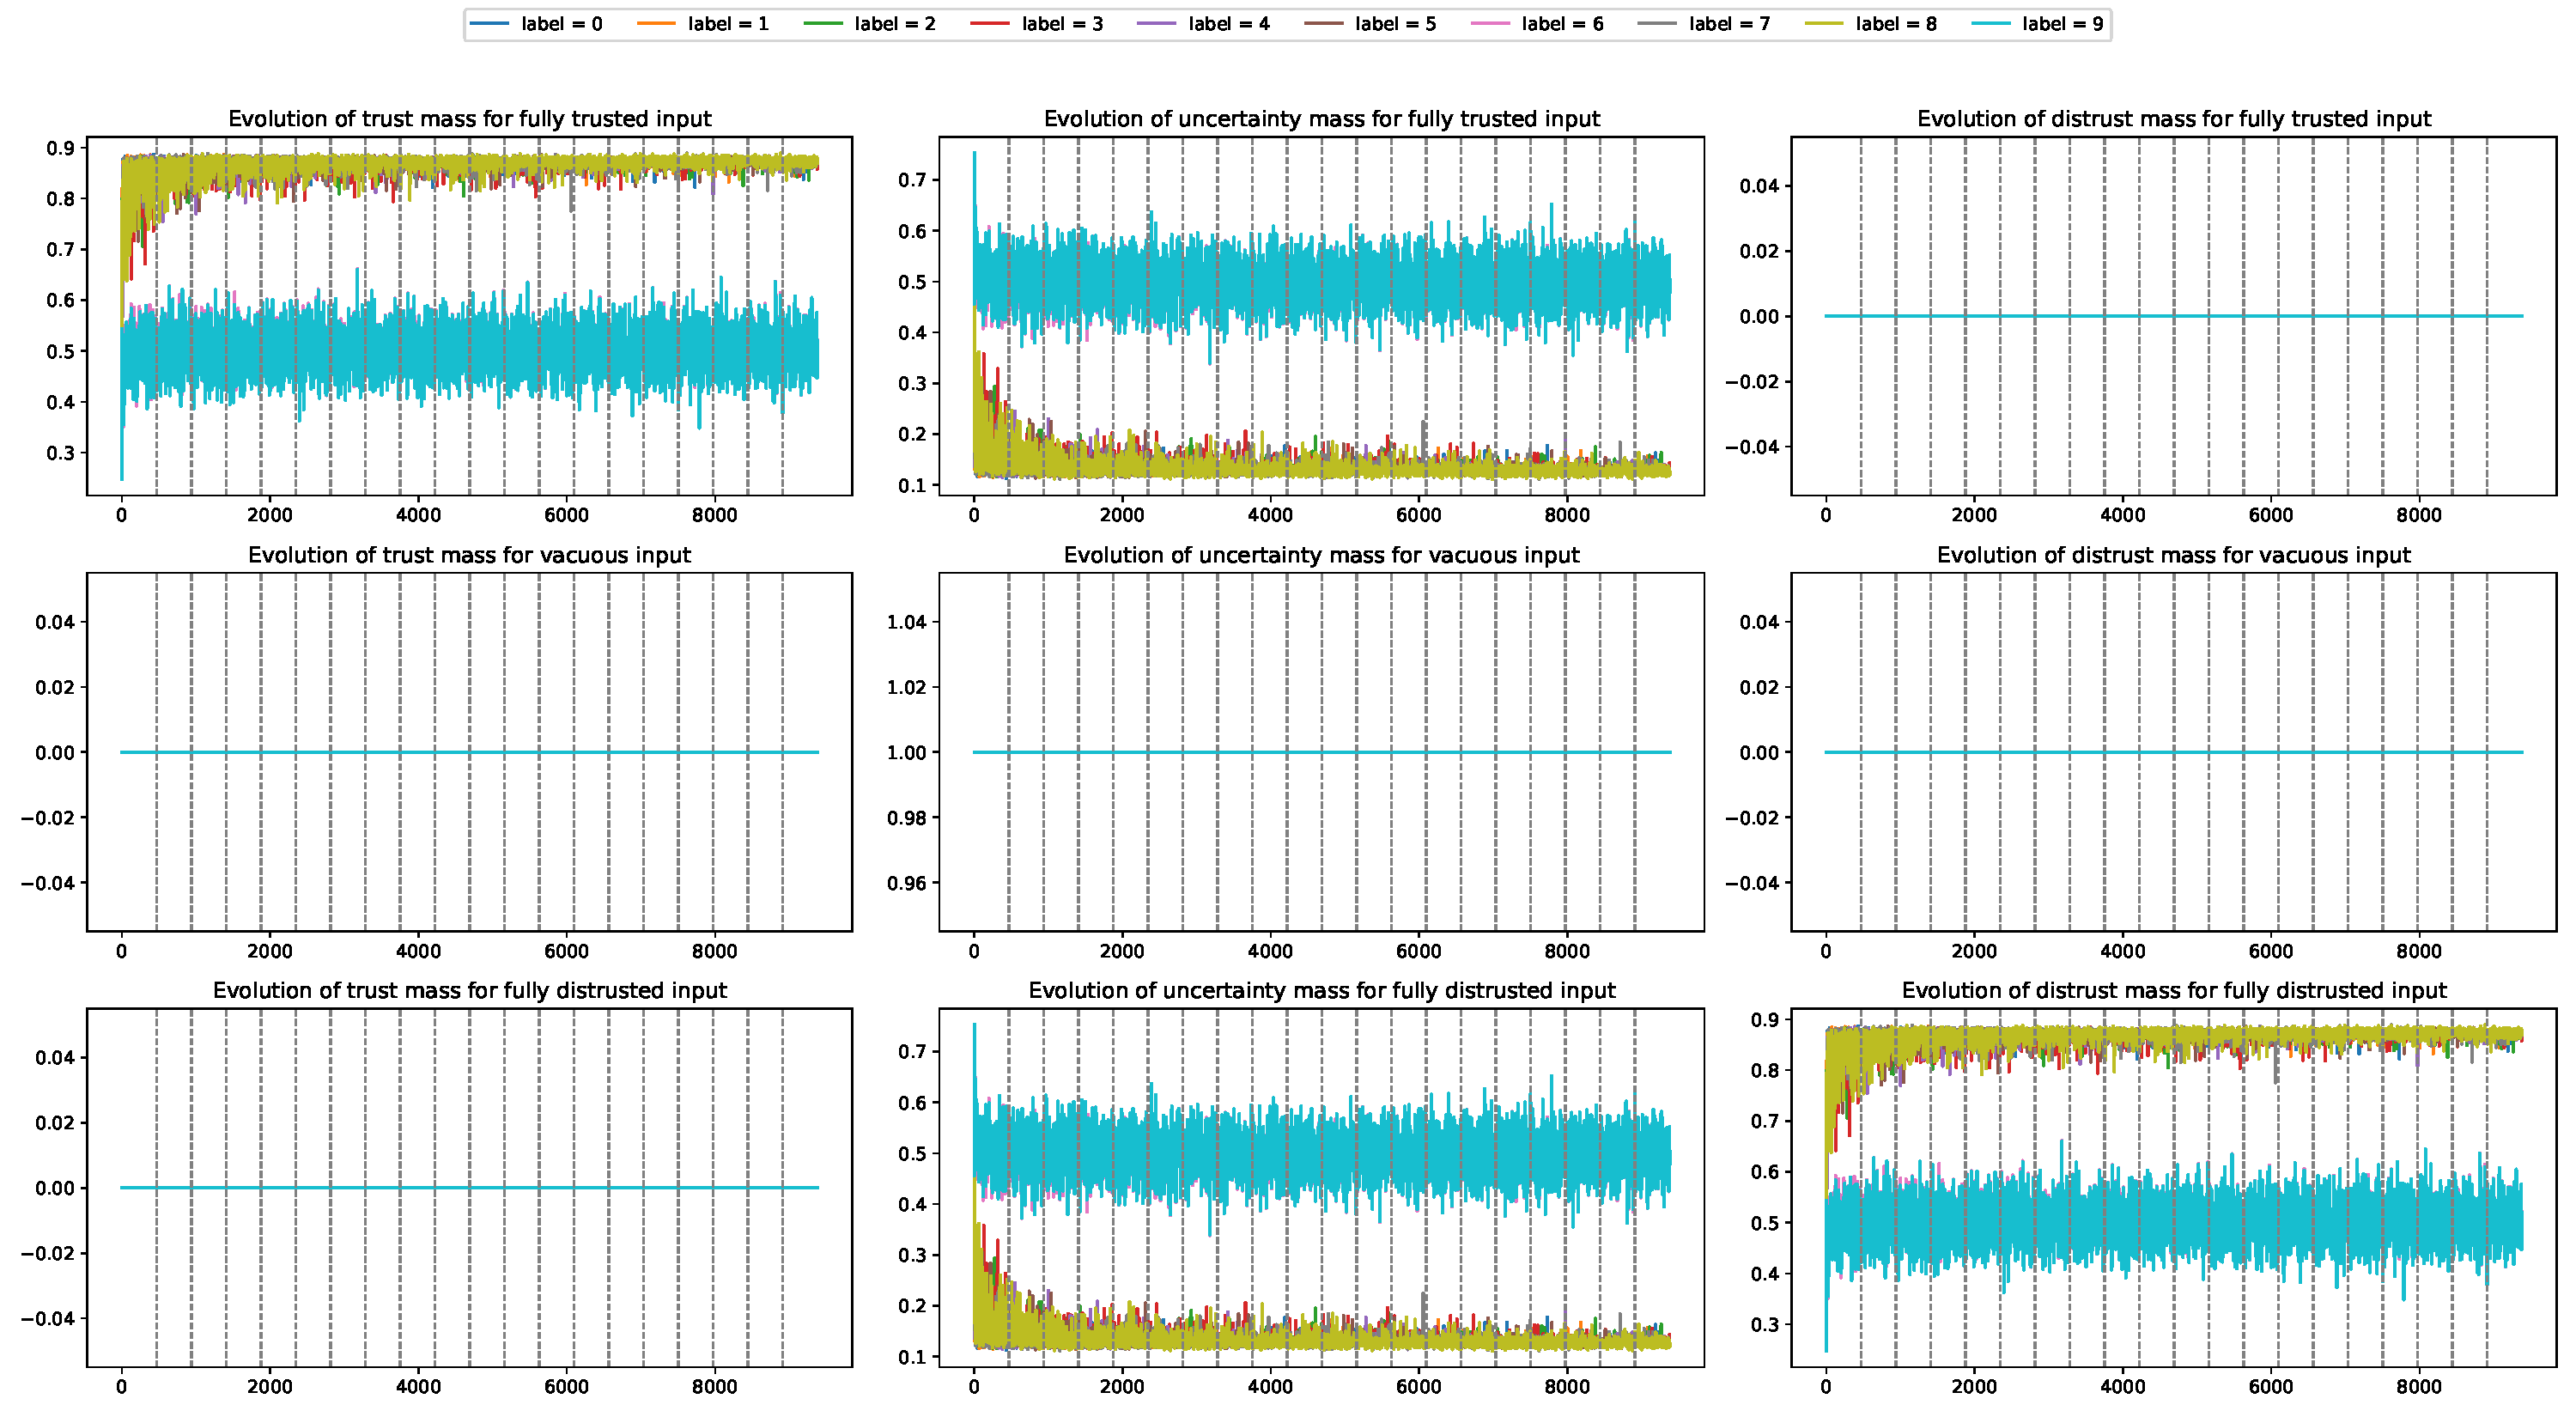
\includegraphics[width=\textwidth]{plots_v2/MNIST/poisoned/plot_ptas-128-t-t-ps10.pdf}
  \caption{10×10 pixels}
\end{figure}
\begin{figure}[H]
  \centering
  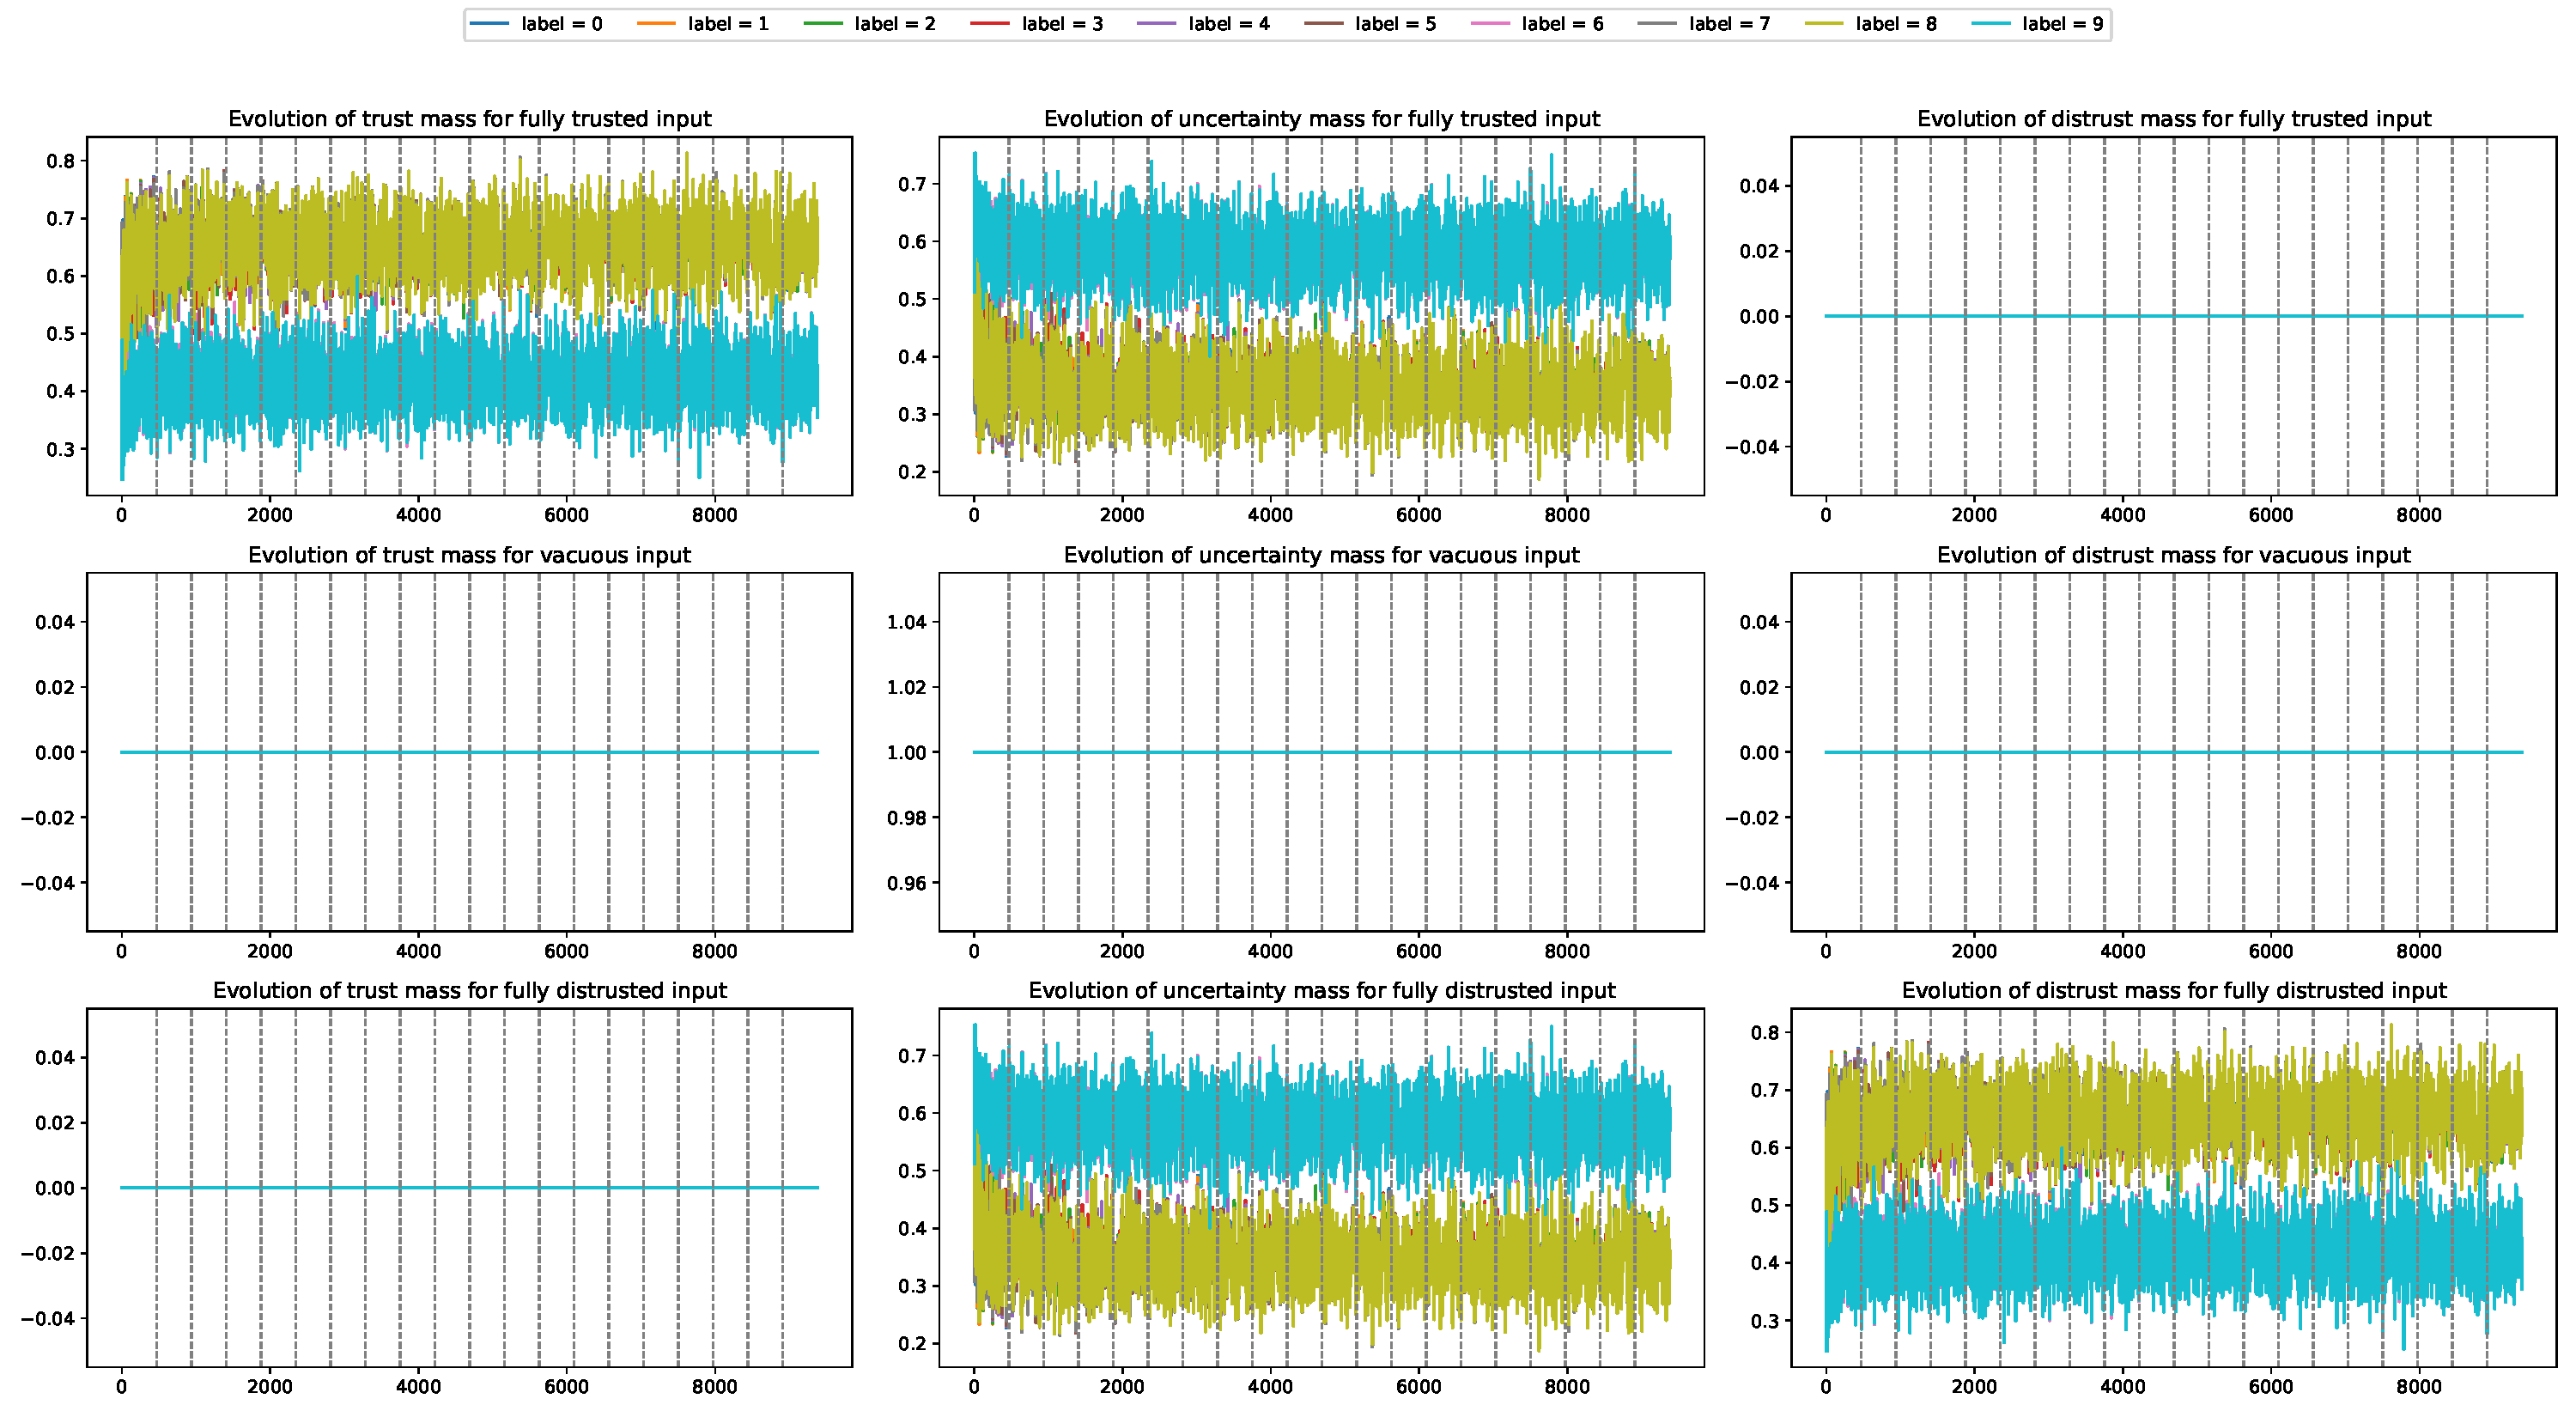
\includegraphics[width=\textwidth]{plots_v2/MNIST/poisoned/plot_ptas-128-t-t-ps27.pdf}
  \caption{27×27 pixels}
\end{figure}
\subsection{Plots for the Comparative Trust Evaluation (\cref{exp:4})}\label{sec:resexp4}
\begin{figure}[H]
  \centering
  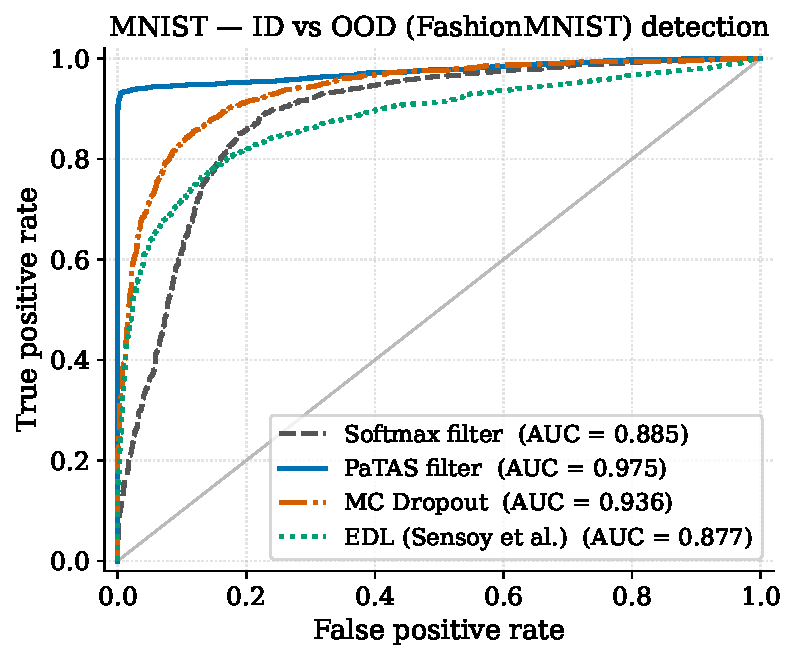
\includegraphics[width=0.62\textwidth]{plots_v2/exp4/roc_ood_mnist.pdf}
  \caption{Out-of-distribution detection ROC (MNIST in-distribution vs.\ Fashion-MNIST OOD): each method's own score as the discriminator. Curves and legend AUC values are from a single representative evaluation seed; \cref{tab:comparative} reports mean $\pm$ std over three seeds.}
\end{figure}
\begin{figure}[H]
  \centering
  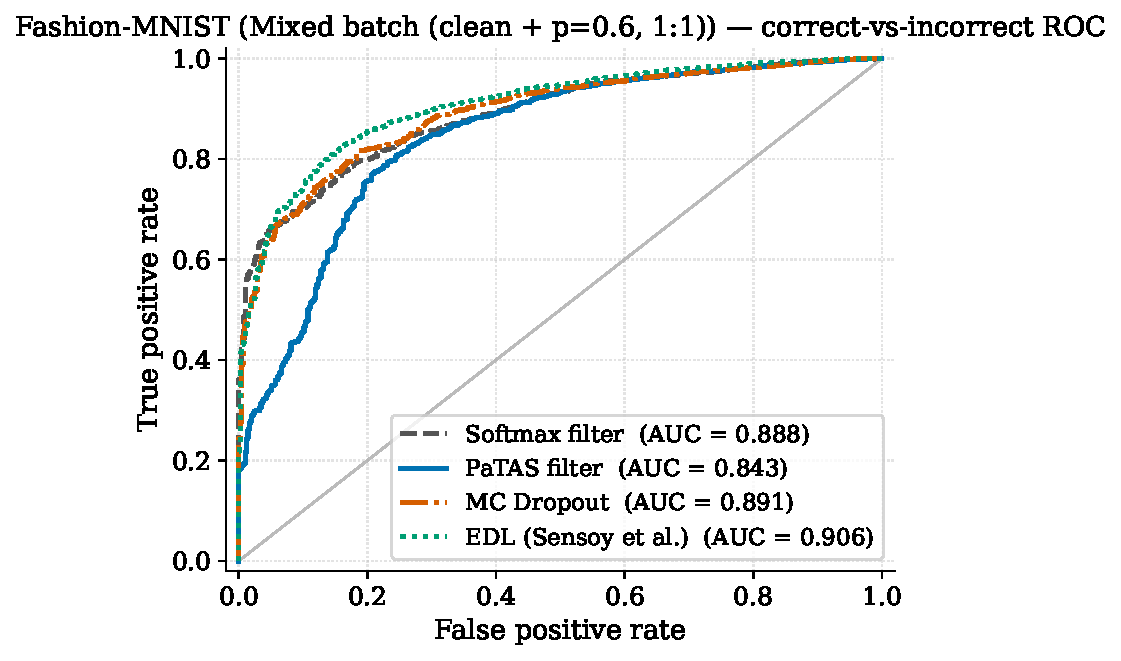
\includegraphics[width=0.62\textwidth]{plots_v2/exp4/roc_mixed_fashion.pdf}
  \caption{Correct-vs-incorrect ROC on the Fashion-MNIST mixed batch (clean + corrupted inputs pooled 1:1), single representative evaluation seed.}
\end{figure}
\begin{figure}[H]
  \centering
  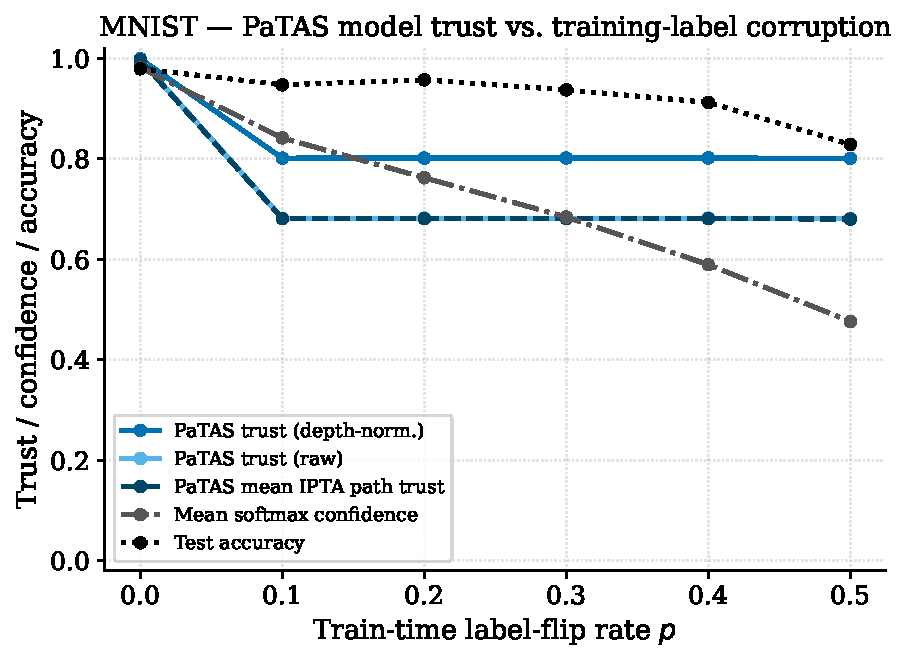
\includegraphics[width=0.62\textwidth]{plots_v2/exp4/model_trust_vs_labelnoise.pdf}
  \caption{Training-quality audit (\cref{tab:audit}): PaTAS model-side trust, mean softmax confidence, and test accuracy as functions of the train-time label-flip rate $p$. The depth-normalized curve rescales the committed mass $b+d$ of the aggregated opinion to $(b+d)^{1/L}$, with $L$ the number of trust-propagation layers, making trust comparable across network depths. Trust drops as a tripwire at any non-zero rate without using test data; confidence tracks severity but requires a clean labelled test set.}
\end{figure}
